% This is LLNCS.DEM the demonstration file of
% the LaTeX macro package from Springer-Verlag
% for Lecture Notes in Computer Science,
% version 2.4 for LaTeX2e as of 16. April 2010
%
\documentclass{llncs}
\usepackage{geometry}
\geometry{
  a4paper,         % or letterpaper
  textwidth=18cm,  % llncs has 12.2cm
  textheight=24cm, % llncs has 19.3cm
  heightrounded,   % integer number of lines
  hratio=1:1,      % horizontally centered
  vratio=2:3,      % not vertically centered
}
\newcommand\tab[1][1cm]{\hspace*{#1}}
\pagestyle{headings}
\usepackage{graphicx, color}
\usepackage{lscape}
\usepackage{listings}
\usepackage{color,soul}
\usepackage{array}
\usepackage{rotating}
\usepackage{amsmath}
\usepackage{multirow}
\usepackage{fixltx2e}
\usepackage[table]{xcolor}
\usepackage[title]{appendix}
\usepackage{algorithm}
\usepackage{makeidx}  % allows for index generation
\usepackage{tablefootnote}
\usepackage{color}   %May be necessary if you want to color links
\usepackage{hyperref}
\hypersetup{
    colorlinks=true, %set true if you want colored links
    linktoc=all,     %set to all if you want both sections and subsections linked
    linkcolor=blue,  %choose some color if you want links to stand out
}

%\makesavenoteenv{tabular}
%
\definecolor{listinggray}{gray}{0.9}
\definecolor{lbcolor}{rgb}{0.9,0.9,0.9}
\lstset{
  backgroundcolor=\color{lbcolor},
  basicstyle=\ttfamily\small,
  basewidth=0.5em,
  showstringspaces=false,
  keywordstyle=\color[rgb]{0,0,1},
  commentstyle=\color[rgb]{0.133,0.545,0.133},
  stringstyle=\color[rgb]{0.627,0.126,0.941},
  breaklines=true,
  frame=lines,
  numbers=left,
  stepnumber=1
}
%
%
%
\title{A Tutorial on TTool/DIPLODOCUS: an Open-source Toolkit for the Design of Data-flow Embedded Systems}
\author{Andrea Enrici\inst{1} \and Letitia Li\inst{2} \and Ludovic
Apvrille\inst{2} \and Dominique Blouin\inst{2}} \institute{Nokia Bell Labs
France\\Centre de Villarceaux, Route de Villejust 91620, Nozay, France\\
\email{andrea.enrici@nokia.com},\\
\and
LTCI, CNRS, Telecom ParisTech, Universit\'{e} Paris-Saclay, 75013, Paris, France\\
\email{\{letitia.li, ludovic.apvrille, dominique.blouin\}@telecom-paristech.fr}
}

\newcommand{\screenshotsize}{1.0\textwidth}


\setcounter{tocdepth}{3}
\begin{document}

\maketitle


\begin{abstract}
TTool/DIPLODOCUS is an open-source Computer Aided Design tool that allows the modeling, verification (simulation and
formal verification) and automatic code generation of data-flow embedded systems, from UML/SysML diagrams.\\
%
This document is a tutorial for TTool/DIPLODOCUS that guides the reader through the complete design of the data-link
layer of a ZigBee transmitter~\cite{ZigBee}. We first provide a short introduction that motivates the use of Electronic
Design Automation and Model-Driven Engineering to facilitate the programming of modern embedded systems. Subsequently,
we present a generic overview of TTool/\-DI\-PLO\-DO\-CUS (Section~\ref{sec:Overview}) and of its software architecture
(Section~\ref{sec:SwArch}). Section~\ref{sec:Config} guides the user through the installation and configuration process.
This is followed by the tutorial that illustrates the full design of the ZigBee transmitter, from modeling
(Section~\ref{sec:Modeling}) to Design Space Exploration (Section~\ref{sec:DSE}) and automatic code generation
(Section~\ref{sec:CodeGen}). Section~\ref{sec:Conclusion} conludes this document.
\end{abstract}
%
\begin{figure}[htbp]
	\centering
	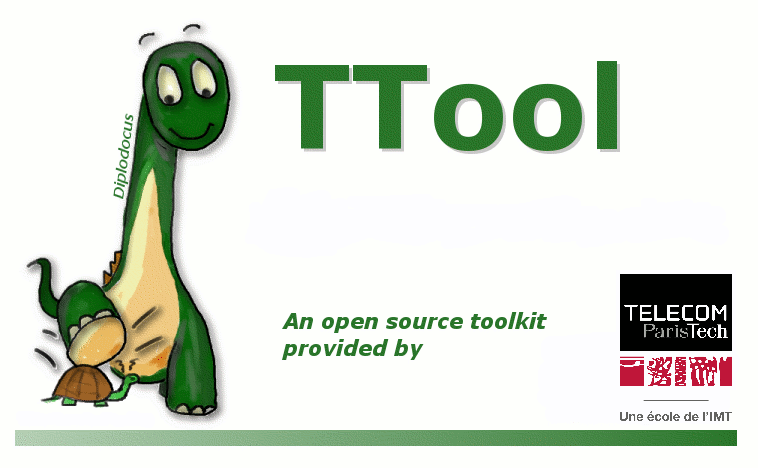
\includegraphics[width=0.7\textwidth]{./figures/TTool.png}
\end{figure}
%
%
%
\newpage
\tableofcontents
\newpage
\section{Important note}
The screen capture provided in this tutorial have been made with a former version of TTool. The graphical interface of the version of TTool you will use to follow this tutorial may thus differ, e.g. you will have to find the corresponding icon in your version. To do so, you can place your mouse over an icon to get an information on it. By doing so, you should be able to locate when icons have been moved.


\newpage
\section{Why TTool/DIPLODOCUS?}
\label{sec:Introduction}
%
To provide more computational power, modern embedded systems are more and more realized as parallel systems where the
processing and control are distributed over a network of interconnected subsystems. This type of architecture is
used for data-flow applications where performance is driven by the need to rapidly process and transfer large volumes
of data (e.g., signal, video and image processing). Currently, we find that parallel and distributed architectures are
largely adopted both at the chip level (e.g., Multi-Processors Systems on Chip) or in domains where the electronic
components are physically distributed over the structure of the entire system (e.g., automotive and avionics domains).
These architectures are intrinsically difficult to program because of their high degree of parallelism, the complex
interactions between hardware and software components, and their heterogeneous nature. They are typically
assembled with components from different vendors (e.g., CPU, RAM motherboard and its communication infrastructure) and
with different characteristics (e.g., memory architecture, Application Programming Interface).\\
%
In this context, an important challenge is to efficiently program and verify these complex platforms, and reduce the
time-to-market of new products, development time and costs.\\
%
Among the possible approaches that can be taken to alleviate software development, Model Driven
Engineering~\cite{Schmidt} proposes to raise the level of abstraction at which these systems are programmed. Instead of
directly encoding a given functionality (e.g., a signal-processing algorithm such as LTE) into code that will be
executed by a target platform, MDE aims to capture this functionality in high-level models that are independent of a
specific target platform or implementation technology. These models are then coupled with transformation engines that
can automatically generate artifacts (e.g., code, documentation) for multiple targets and implementations.\\
%
To design an embedded system, traditionally an engineer separately models both the application(s) - i.e., the functional
part of the system - and the candidate platform - i.e., the hardware/software resources - with the assistance of
dedicated Electronic Design Automation (EDA) tools. Then he/she selects (\textit{maps}) the platform units that will
execute the function's workload. The resulting design, given by the mapping model, is evaluated in terms
of performance (e.g., power consumption, throughput, latency, silicon area occupation) and compared to a set of
requirements. In case of a positive match, an implementation (i.e, compilable software, synthesizable hardware) is
generated via automatic model transformations. In case of a negative match, the application and platform models are
iteratively improved, mapped and evaluated until the resulting design complies with the desired requirements.
%() finding a mapping solution compliant to some performance requirements is typically an iterative process: performance
%numbers are first extracted from mapping models. Then, according to these numbers, pre-mapping models are improved and
%the process starts over until performance numbers converge to the desired performance requirements.
This design process is known as the Y-chart approach~\cite{YChart} and is shown in Fig.~\ref{fig:Ychart}.
%
\begin{figure}[htbp]
	\centering
	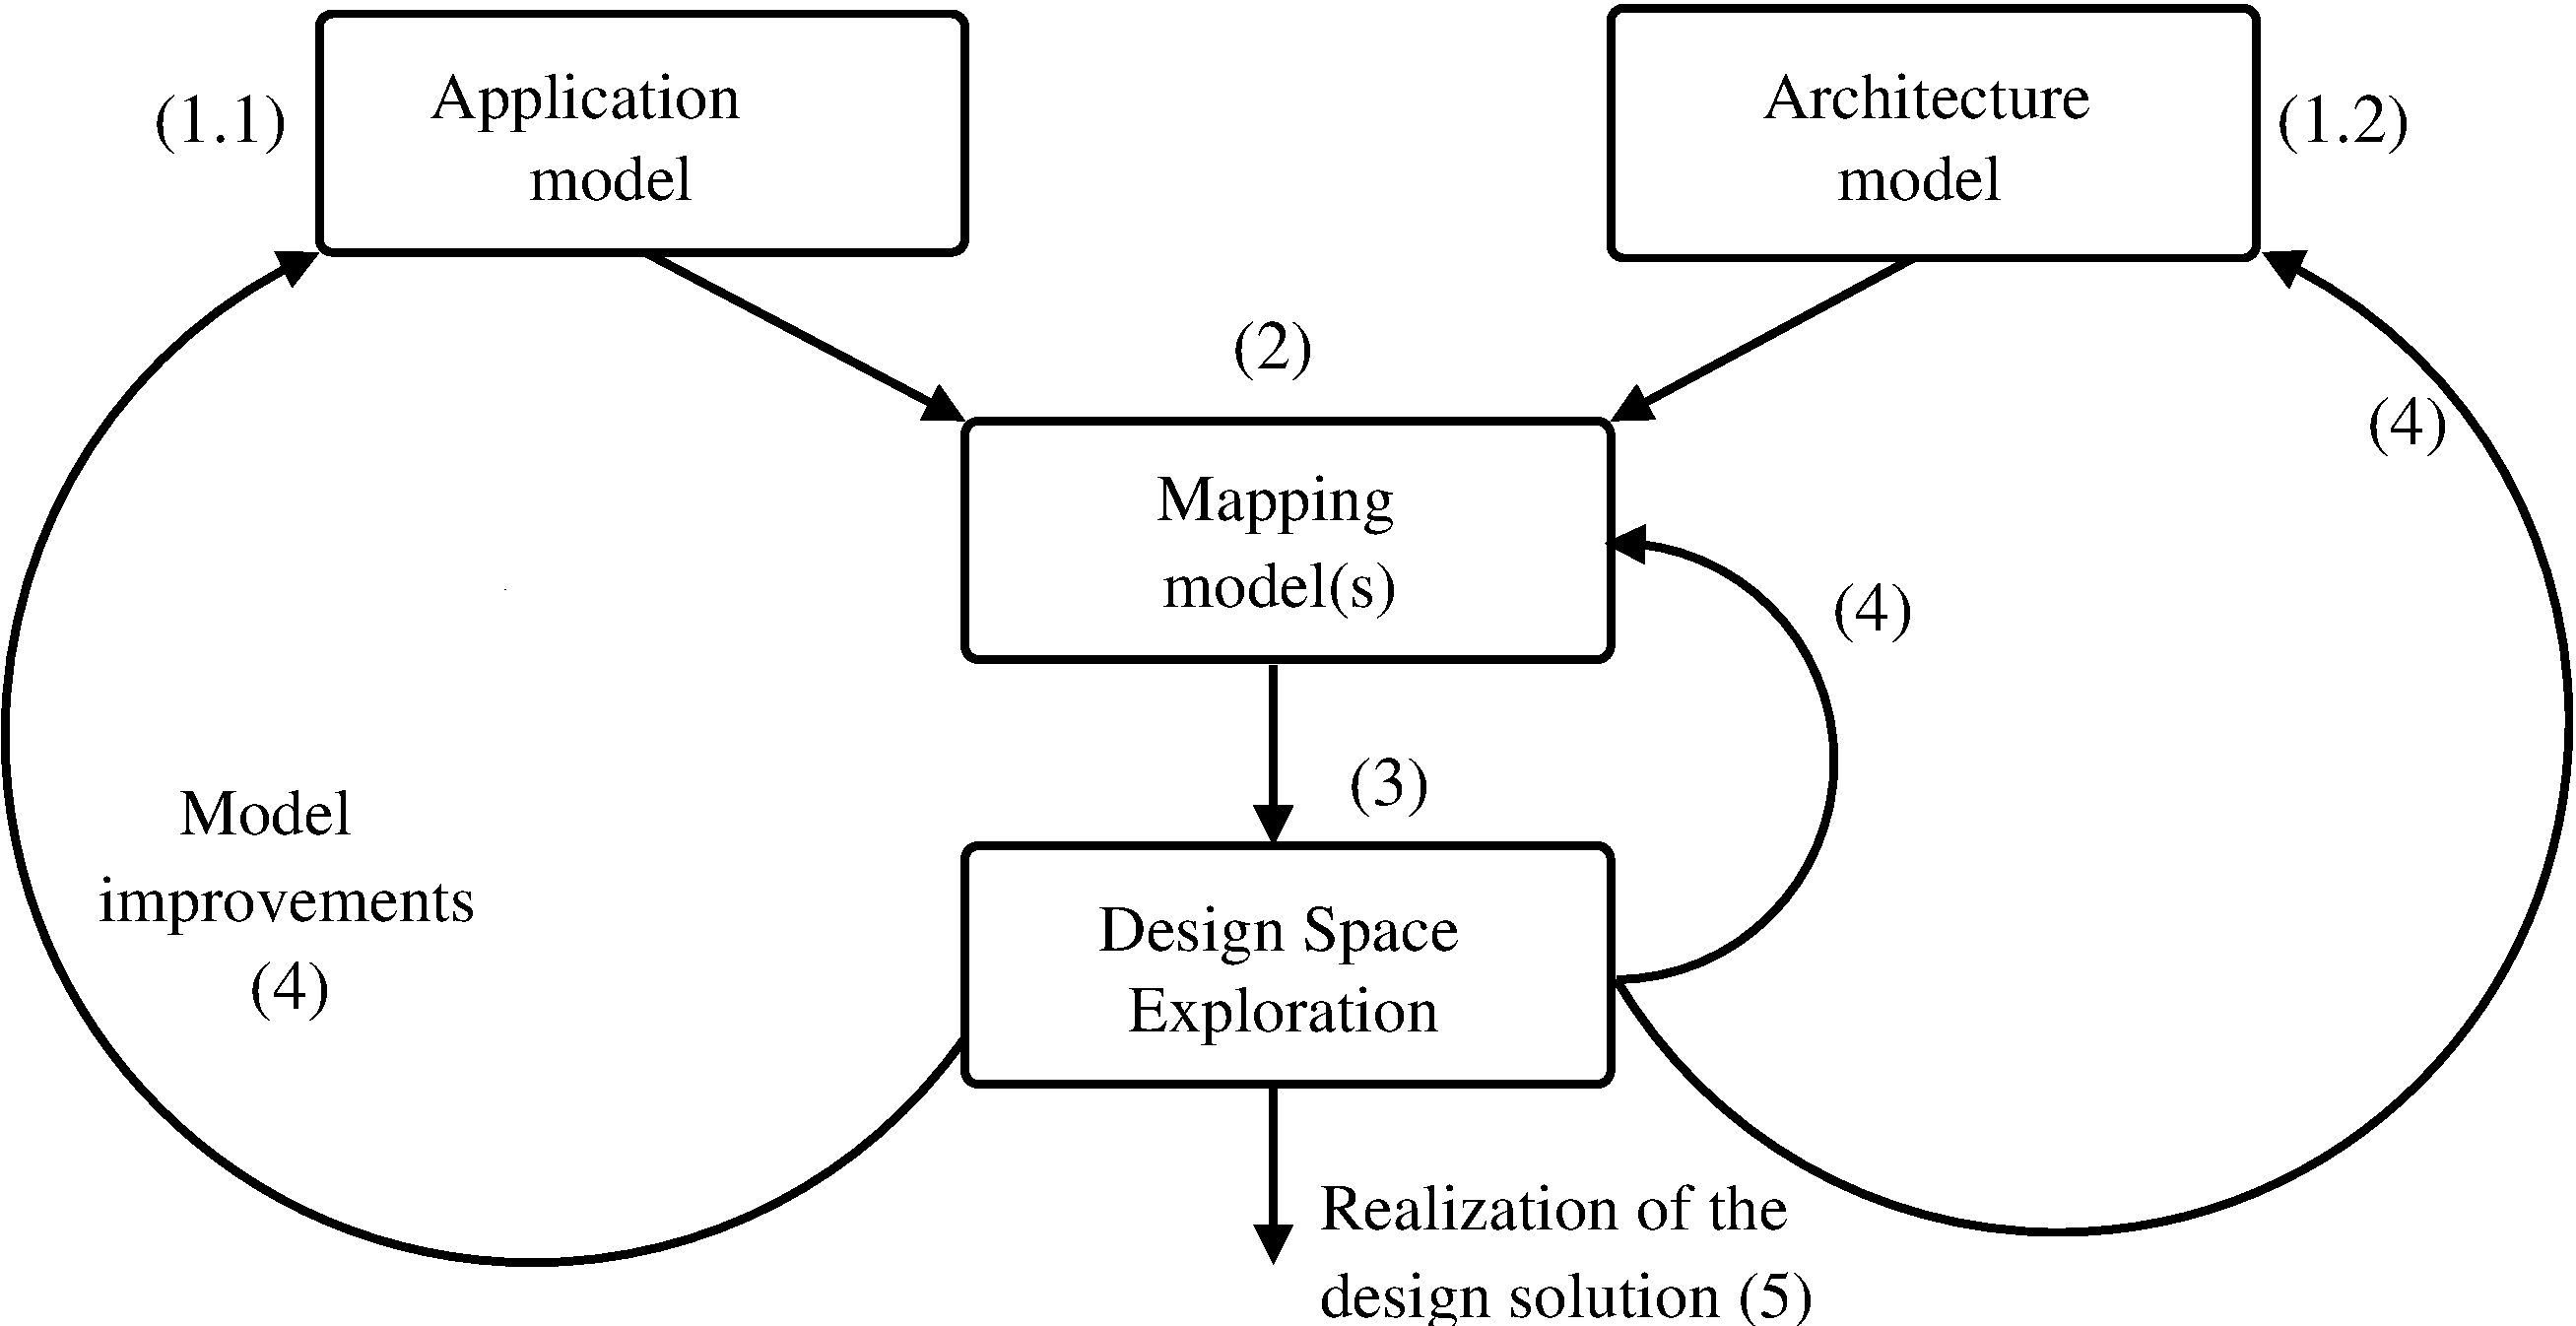
\includegraphics[width=0.55\textwidth]{./figures/ApproachY.pdf}
	\caption{The Y-chart approach for the design of programmable embedded systems}
	\label{fig:Ychart}
\end{figure}
%
\section{An overview of TTool/DIPLODOCUS}
\label{sec:Overview}
%
TTool/DIPLODOCUS is an open-source EDA toolkit dedicated to the design of data-flow embedded systems based on UML and
SysML diagrams. To go into more detail, TTool is the name of the toolkit and DIPLODOCUS is the name of a specific UML/SysML
profile dedicated to the partitioning of embedded systems. TTool also supports the AVATAR, TURTLE, SysML-Sec, CTTool and
Network Calculus profiles~\cite{TToolWebSite}. TTool/DIPLODOCUS~\cite{Apvrille06},~\cite{Apvrille08}~\cite{TToolWebSite}
uses an evolution of the Y-chart approach that is called the $\Psi$-chart approach, shown in Fig.~\ref{fig:Tchart}. In
the $\Psi$-chart approach, a third set of input models is introduced to capture communication protocols and patterns
(step 1.3 in Fig.~\ref{fig:Tchart}) independently of the application and platform models. This has proven to reduce the
design time in terms of the number of iterations in the Model improvement phase (step 4 in Fig.~\ref{fig:Ychart} and in
Fig.~\ref{fig:Tchart}) as well as to improve the portability of models~\cite{EnriciThesis} to target multiple
platforms.
%
\begin{figure}[htbp]
	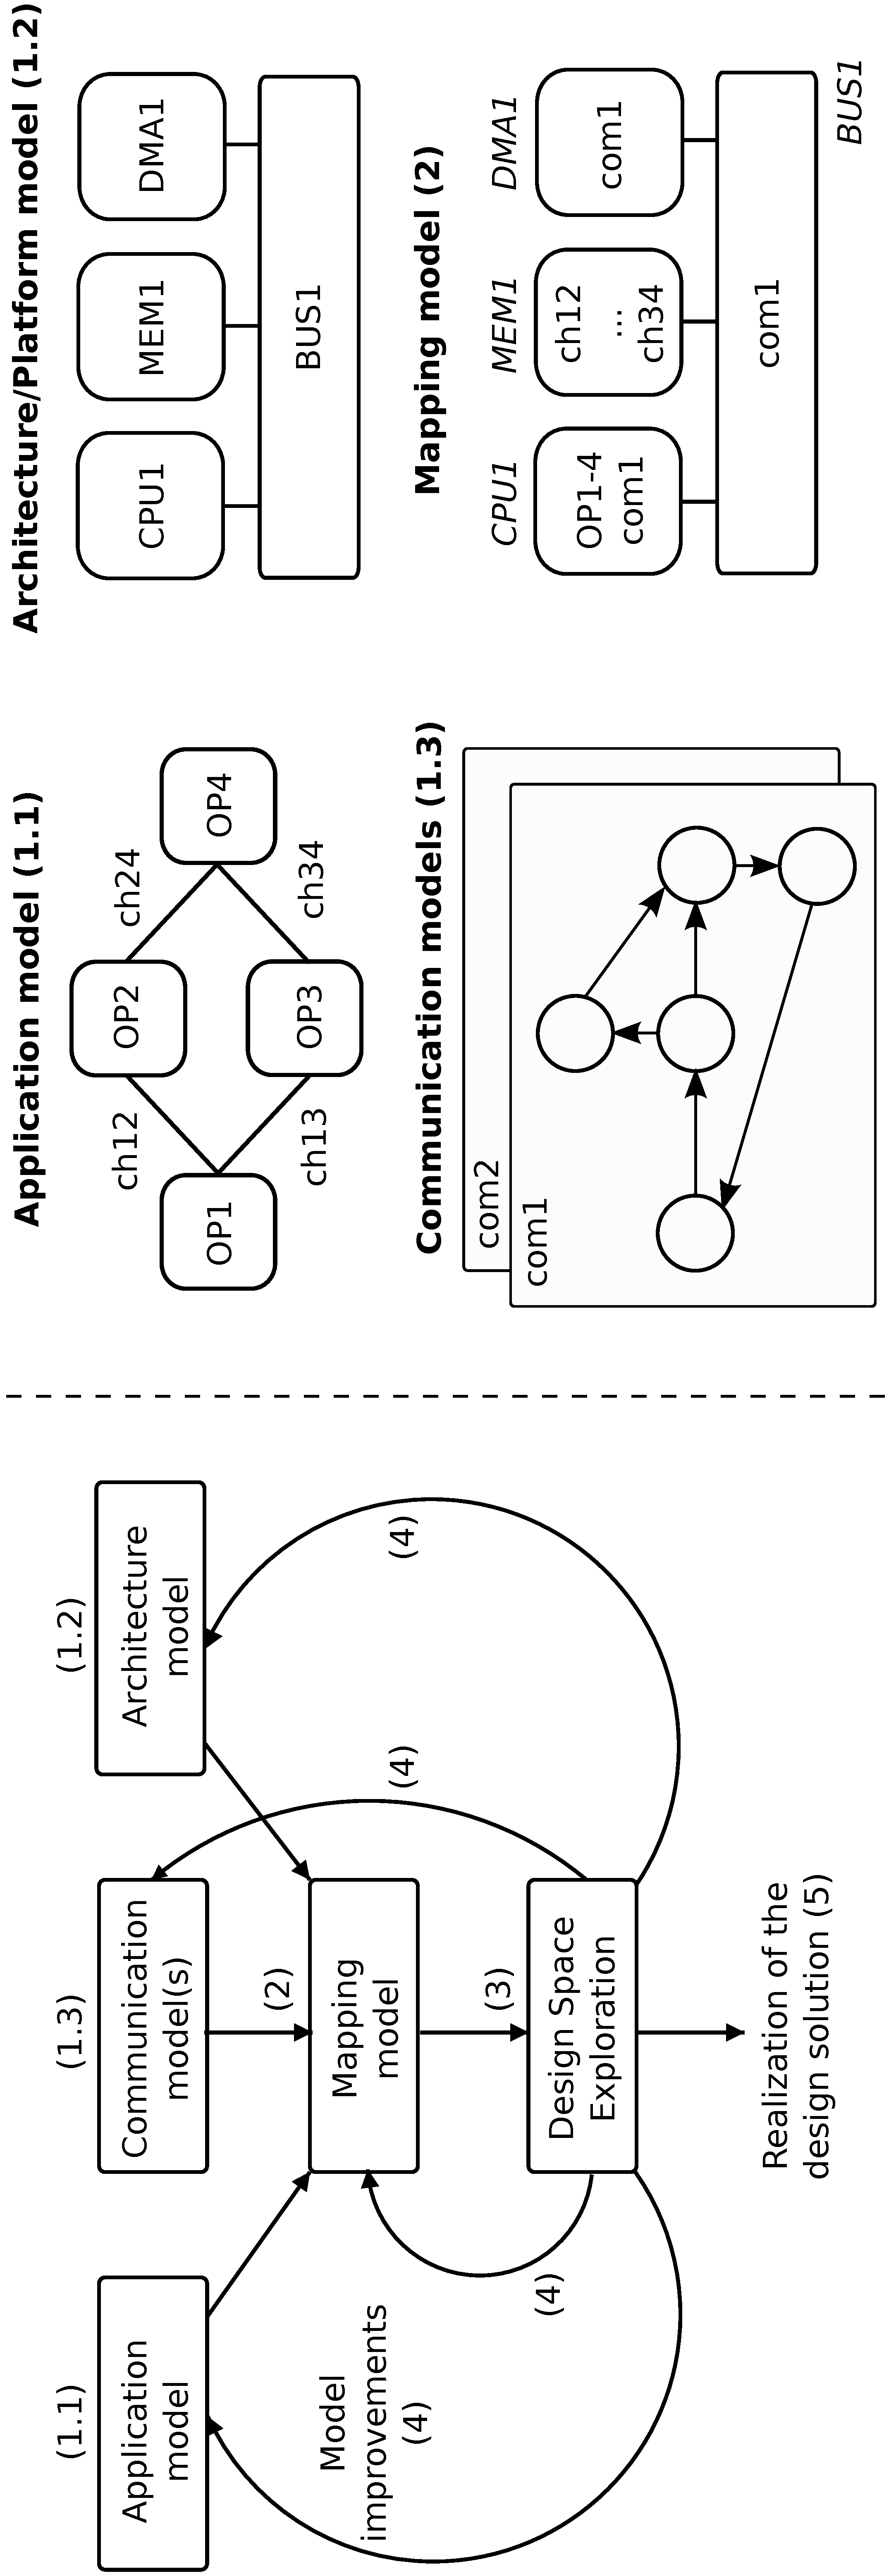
\includegraphics[angle=-90,origin=c,width=\textwidth]{figures/applicationModel.pdf}
	\vspace{-17em}
	\caption{The $\Psi$-chart approach (left side) and a graphical visualization of its constituent models (right
side).}
	\label{fig:Tchart}
\end{figure}
%
\\In TTool/DIPLODOCUS, an \textit{application} model (step 1.1 in Fig.~\ref{fig:Tchart}) is denoted with SysML Block
Definition and Activity diagrams. An application is described as a set of blocks interconnected by data and control
dependencies via ports and channels. The internal behavior of each block is described by a SysML Activity Diagram. An
application model is based on the two following abstraction principles:
%
\begin{itemize}
	\item \emph{Data abstraction:} only the amount of data exchanged between application blocks is modeled. Internal
	decisions that depend on the value of data are expressed in terms of non-deterministic and static operators (i.e.,
	conditional choice based on the value of a random variable).
	%
	\item \emph{Functional abstraction:} algorithms are described using abstract cost operators that express the
	complexity of processing data in terms of the number of operations required to execute them (e.g., number of integer
	operations).
\end{itemize}
%
A \textit{platform} model (step 1.2 in Fig.~\ref{fig:Tchart}) is denoted using a UML Deployment Diagram that represents
a set of generic interconnected resources, e.g., bus, CPU and its operating system, DMA, memory. These resources are
characterized by performance and implementation parameters (e.g., the scheduling policy and the number of cores for a
CPU, the addresses of memory areas) that are used for Design Space Exploration (DSE), evaluation (e.g., simulation, formal
verification), and to realize a design solution (i.e., control code synthesis). A \textit{communication} model (step 1.3
in Fig.~\ref{fig:Tchart}) is denoted using SysML Activity Diagrams and UML Sequence Diagrams that represent,
respectively, the algorithm of a communication protocol and the entities (e.g., master, slave) that are involved in
exchanging information. A \textit{mapping} model (step 2 in Fig.~\ref{fig:Tchart}) is created from an instance of the
platform model where dedicated UML artifacts are added to map computations and communications. The abstract cost
operators are assigned a value according to the performance characteristics (e.g., operating frequency) of the
platform's units. TTool/DIPLODOCUS allows a user to map functions that belong to different functional views (i.e.,
application models) and to different communication models.\\
%
Design Space Exploration in TTool/DIPLODOCUS (step 3 in Fig.~\ref{fig:Tchart}) evaluates the performance of a mapping
solution by simulating the workload of computations and data-transfers~\cite{Knorreck11}. A formal verification
engine~\cite{Knorreck11} is also available to verify system properties (e.g., liveness, reachability, scheduling). DSE
can be performed both manually via the tool's GUI or automatically via a set of scripts that configure the DSE engine to
evaluate different mapping alternatives.\\
%
The realization of a design solution in TTool/DIPLODOCUS (step 5 in Fig.~\ref{fig:Tchart}) is possible in terms of a
software implementation, via the automatic generation of control code. This code corresponds to the functionality of
the application and communication models as mapped onto dedicated resources of the platform model. From a software
viewpoint, this control code is an application that runs on top of the Operating System of a general-purpose processor
in the target platform.\\
%
The abstraction principles underlying models of TTool/\-DI\-PLO\-DO\-CUS answer the need to target early design and DSE,
when not all the details about a system's application (e.g., value and type of data) and platform (e.g., Operating
System, size and policy of cache memories for a CPU) are known. The validation of the effectiveness of these
abstractions has been described in~\cite{Jaber2011}, where TTool/DIPLODOCUS was used for the design of the physical
layer of a LTE base station jointly with Freescale Semiconductors. The resulting design in TTool/\-DI\-PLO\-DO\-CUS lead
to performance results that differed by only 10\% with respect to the final implementation. To obtain these performance
figures, design in TTool/\-DI\-PLO\-DO\-CUS required only a few weeks, whereas manual development of a functionally
equivalent system amounted to 6 months.
%
%
%
\section{The software architecture of TTool/DIPLODOCUS}
\label{sec:SwArch}
%
Fig.~\ref{fig:TToolSWArch} illustrates the software architecture of TTool that is relevant to the DIPLODOCUS profile.
Most of the software that composes TTool is developed in Java, except for the Design Space Exploration engine that has
been developed in C++ for performance reasons.\\
%
The topmost level of Fig.~\ref{fig:TToolSWArch} shows the Diagram Editor, an in-house Java Graphical User
Interface that permits designers to draw UML/SysML diagrams. Graphical models are first converted into an Intermediate
Format (IF) Java data structure (Models-to-data-structure Transformation, Intermediate Format in
Fig.~\ref{fig:TToolSWArch}). This software data structure constitutes a common layer from which models are transformed
for DSE via formal verification, simulation and for implementation via the synthesis of executable control code.\\
%
TTool/DIPLODOCUS also accepts as input a textual representation of a design, specified in a dedicated language called
Task Modeling Language (TML)~\cite{Waseem06}. This TML representation, Fig.~\ref{fig:TToolSWArch}, is manually input by
the user, as an alternative to UML/SysML diagrams. Instead, when the latter are used, a TML description can be
automatically produced from the IF data structure, Fig.~\ref{fig:TToolSWArch}.
%
\begin{figure}[!htbp]
	\centering
	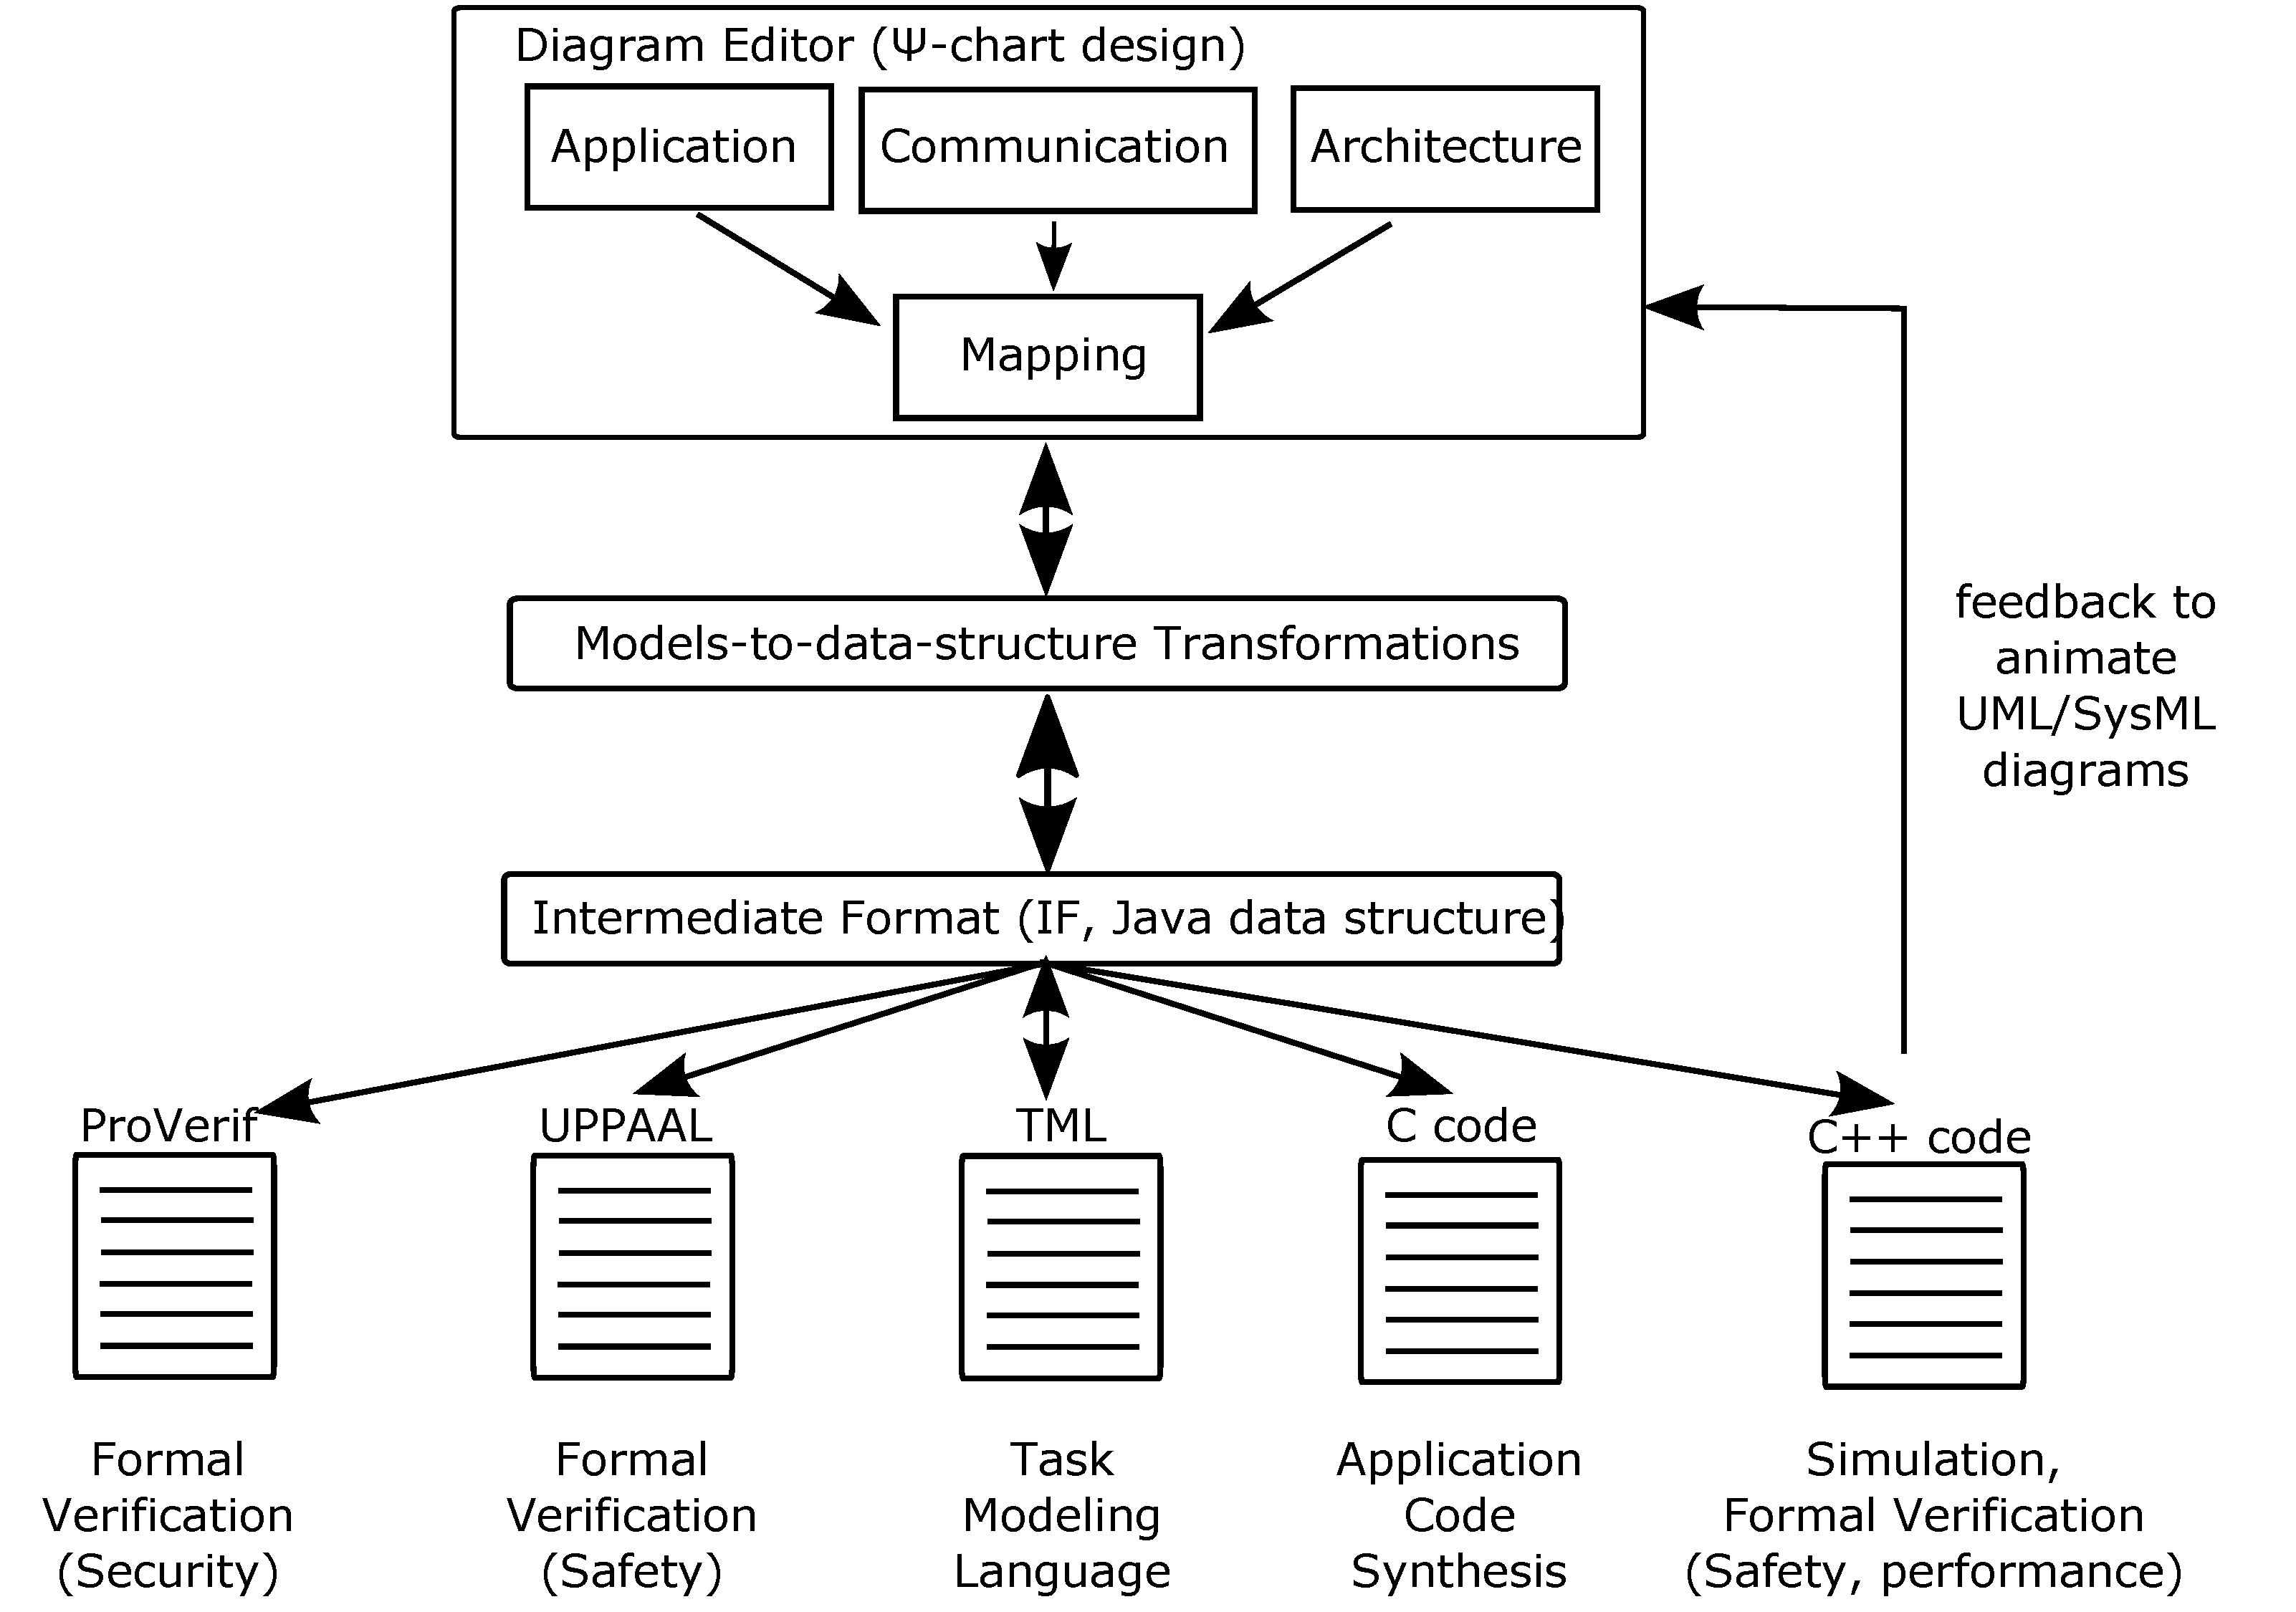
\includegraphics[width=4in]{figures/TToolSWArch.pdf}
	\caption{The software architecture of TTool for the UML/SysML profile DIPLODOCUS}
	\label{fig:TToolSWArch}
\end{figure}
%
%
%
\section{Configuring TTool/DIPLODOCUS}
\label{sec:Config}
%
In this section, we describe the steps that are necessary to install and configure TTool/DIPLODOCUS in a Linux
environment.\\
%
The source files of TTool can be downloaded in form of a \texttt{.tgz} archive from the website\\
\url{http://ttool.telecom-paristech.fr/download.html}, after having accepted the
licence agreement. To install the tool, simply unpack the archive in your home directory:\\
%

\noindent
\$ \texttt{cd}\\
\$ \texttt{tar -xzvf releaseTToolWithSrc\_RELEASENUMBER.tgz}\\
%

\noindent A folder named TTool will be created in your home directory. A
preconfigured version of the tool can be downloaded from the website and a
version of TTool inside a Virtual Machine is also available upon request to
\href{mailto:ludovic.aprille@telecom-paristech.fr}{ludovic.aprille@telecom-paristech.fr}.
In case the user wants to customize the configuration of TTool, a dedicated
configuration file, \texttt{config.xml} located in
\texttt{your-home/TTool/bin/>}, must be modified as follows:\\
\begin{landscape}
\lstset{basicstyle=\tiny,language=XML}
\begin{lstlisting}
<?xml version="1.0" encoding="ISO-8859-1" ?>"
<TURTLECONFIGURATION>
<RTLHost data="localhost" />
<RTLPath data="your-local-path-to rtl" />
<DTA2DOTPath data="your-local-path-to dta2dot" />
<RG2TLSAPath data="your-local-path-to rg2tlsa" />
<RGSTRAPPath data="your-local-path-to rgstrap" />
<DOTTYPath data="your-local-path-to dotty" />
<DOTTYHost data="localhost" />
<AldebaranHost data="localhost" />
<AldebaranPath data="your-local-path-to aldebaran" />
<BcgioPath data="your-local-path-to bcg\_io" />
<BcgminPath data="your-local-path-to bcg\_min" />
<BisimulatorPath data="your-local-path-to bcg\_open" />
<BcgmergePath data="your-local-path-to bcg\_merge" />
<CaesarPath data="your-local-path-to caesar" />
<CaesarOpenPath data="your-local-path-to caesar.open" />
<FILEPath data="your-home/TTool/modeling" />
<LIBPath data="your-home/TTool/lib" />
<IMGPath data="your-home/TTool/figure" />
<LOTOSPath data="your-home/TTool/lotos" />
<GGraphPath data="your-home/TTool/graphs" />
<TGraphPath data="your-home/TTool/graphs" />
<TToolUpdateURL data="" data1="http://labsoc.comelec.enst.fr/turtle/ttoolversion.html" />
<TToolUpdateProxy data="false" />
<TToolUpdateProxyPort data="8080" />
<TToolUpdateProxyHost data="To Be Completed" />
<JavaCodeDirectory data="your-home/TTool/javacode" />
<JavaCompilerPath data="/usr/bin/javac" />
<TToolClassPath data="your-home/TTool/javacode" />
<JavaExecutePath data="/usr/bin/java" />
<JavaHeader data="import java.sql.*;" />
<SystemCCodeDirectory data="your-home/TTool/simulators/c++2/" />
<SystemCHost data="localhost"/>
<SystemCCodeCompileCommand data="make -C your-home/TTool/simulators/c++2/" />
<SystemCCodeExecuteCommand data="your-home/TTool/simulators/c++2/run.x -ovcd your-home/TTool/simulators/c++2/vcddump.vcd" />
<SystemCCodeInteractiveExecuteCommand data="your-home/TTool/simulators/c++2/run.x -server" />
<TMLCodeDirectory data="your-home/TTool/tmlcode" />
<CCodeDirectory data="your-home/TTool/ccode" />
<GTKWavePath data="/opt/local/bin/gtkwave" />
<VCDPath data="you-home/TTool/vcd/" />
<UPPAALCodeDirectory data="your-home/TTool/uppaal/" />
<UPPAALVerifierPath data="your-home/TTool/uppaal/bin-Linux/verifyta" />
<UPPAALVerifierHost data="localhost" />
<ProVerifCodeDirectory data="your-home/TTool/proverif/" />
<ProVerifVerifierPath data="your-local-path-to proverif" />
<ProVerifVerifierHost data="localhost" />
<AVATARExecutableCodeDirectory data="your-home/TTool/executablecode/" />
<AVATARMPSoCCodeDirectory data="your-home/TTool/MPSoC/" />
<AVATARMPSoCCompileCommand data="make -C your-home/TTool/MPSoC updategeneratedcode compilesoclib" />
<AVATARExecutableCodeHost data="localhost"/>
<AVATARExecutableCodeCompileCommand data="make -C your-home/TTool/executablecode" />
<AVATARExecutableCodeExecuteCommand data="your-home/TTool/executablecode/run.x" />
<AVATARExecutableSoclibCodeCompileCommand data="make -C your-home/TTool/MPSoC updategeneratedcode compilesoclib" />
<AVATARExecutableSoclibCodeExecuteCommand data="make -C your-home/TTool/MPSoC runsoclib" />
<AVATARExecutableSoclibCodeTraceCommand data="make -C your-home/TTool/MPSoC runsoclib-trace" />
<AVATARExecutableSoclibTraceFile data="your-home/TTool/Prog/soclib/soclib/platform/topcells/caba-vgmn-mutekh\_kernel\_tutorial/trace" />
<ExternalCommand1Host data="localhost"/>
<ExternalCommand1 data="an-external-command-of-your-choice, e.g., /opt/local/bin/gtkwave your-local-path-to-a-simulation-trace"/>
<ExternalCommand2Host data="localhost"/>
<ExternalCommand2 data="an-external-command-of-your-choice"/>
<LastOpenFile data="the-path-of-your-last-opened-TTool-file"/>
<LastWindowAttributes x="1097" y="89" width="1075" height="848" max="false" />
<ProVerifHash data=""/>
</TURTLECONFIGURATION>
\end{lstlisting}
\end{landscape}
%
\noindent
TTool can also run on a Windows PC: a dedicated folder located under \texttt{TTool/preinstallTTool/windows} contains the
executable file \texttt{ttool.bat} that directly launches the tool.\\
%
Once the configuration file has been modified, to start TTool, we recommend the user create an executable script
called \texttt{ttool.exe} in the installation directory of TTool, \texttt{<your-home>/TTool/}:\\
%


\noindent
\$ \texttt{touch your-home/TTool/ttool.exe}\\
\$ \texttt{echo "\#! /bin/sh" > your-home/TTool/ttool.exe}\\
\$ \texttt{echo "java -Xmx1024m -jar your-home/TTool/bin/ttool.jar -config your-home/TTool/bin/config.xml\\-avatar -uppaal -launcher" >>
/TTool/ttool.exe}\\
\$ \texttt{chmod u+x your-home/TTool/ttool.exe}\\
%

\noindent
Running the script file will launch the GUI of TTool:\\
%

\noindent
\$ \texttt{./your-home/TTool/ttool.exe}
%
%
%
\newpage
\section{Starting a new project}
\label{sec:Project}
%
To create a new project, click on the \texttt{New} icon shown in Fig.~\ref{fig:CreatePrj} or select \texttt{File->New}
from the Main menu tab. For ease of use, many options from the main menu, such as the creation of a new project, have a
corresponding button in the Button tab.
%
\begin{figure}[htbp]
	\centering
	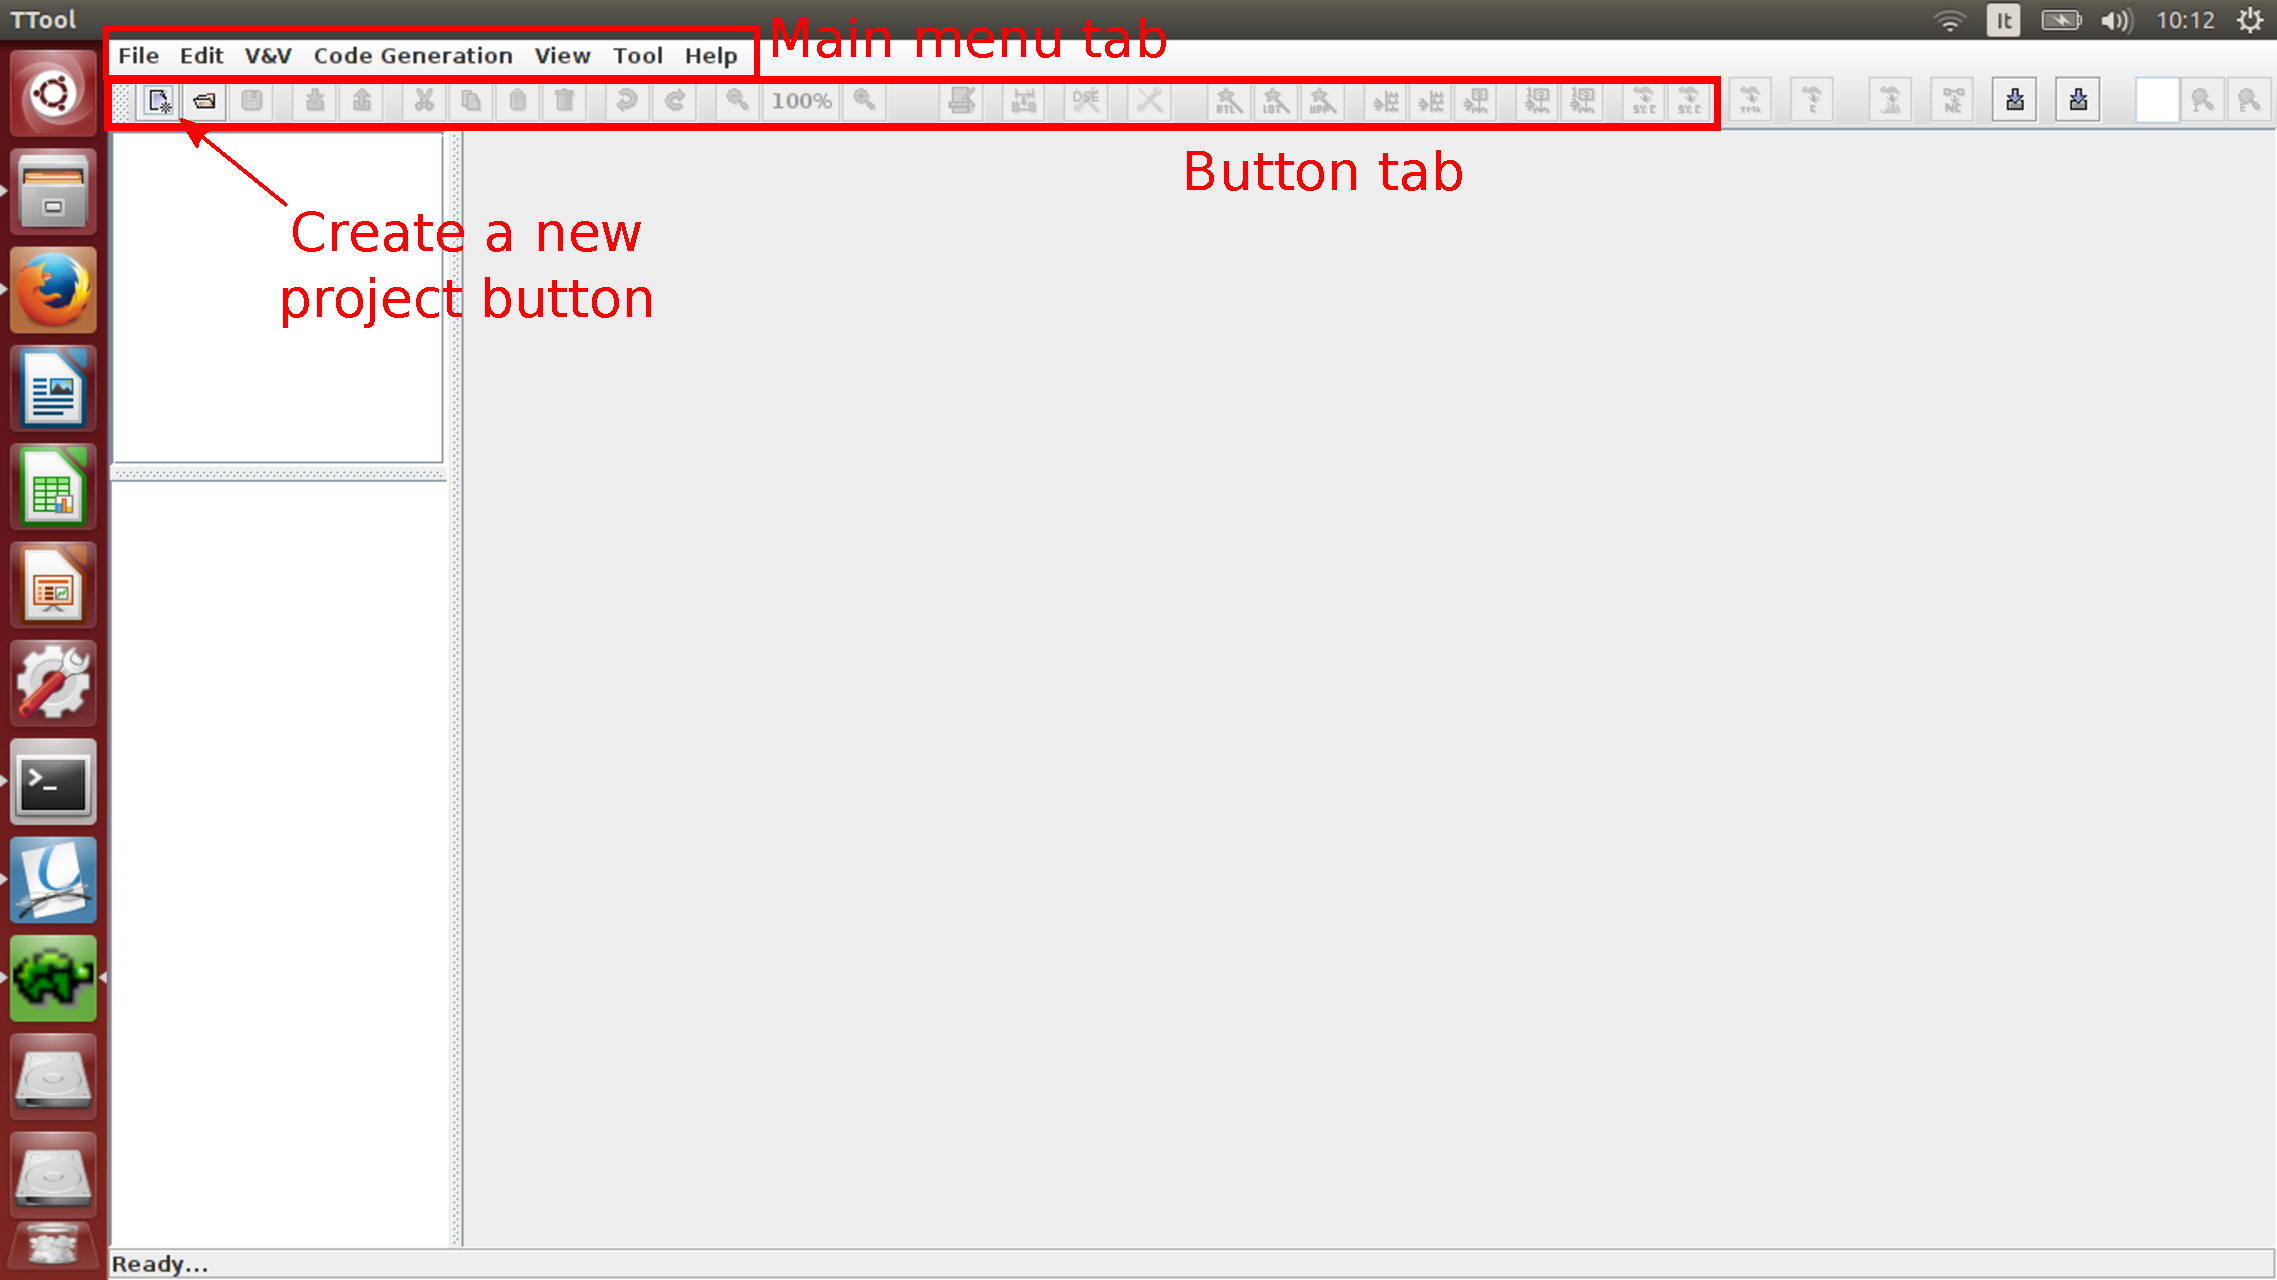
\includegraphics[width=\screenshotsize]{./figures/screenshot/begin.pdf}
	\caption{Create a new project in TTool/DIPLODOCUS}
	\label{fig:CreatePrj}
\end{figure}
%
\\Fig.~\ref{fig:NewPrj} shows the main window of TTool/DIPLODOCUS as it appears after creating a new project. It is
divided into three areas: the Project navigation window, the Map-view window and the Design window. The Project navigation
window allows a user to navigate through the files of a project, to check for results of the syntax analysis and to
rapidly search for elements of a design. The Design window is the window where the UML/SysML diagrams of a design
will be displayed. The Map-view window shows a bird's eye view of the diagram that is currently displayed in the Design
window.
%
\begin{figure}[htbp]
	\centering
	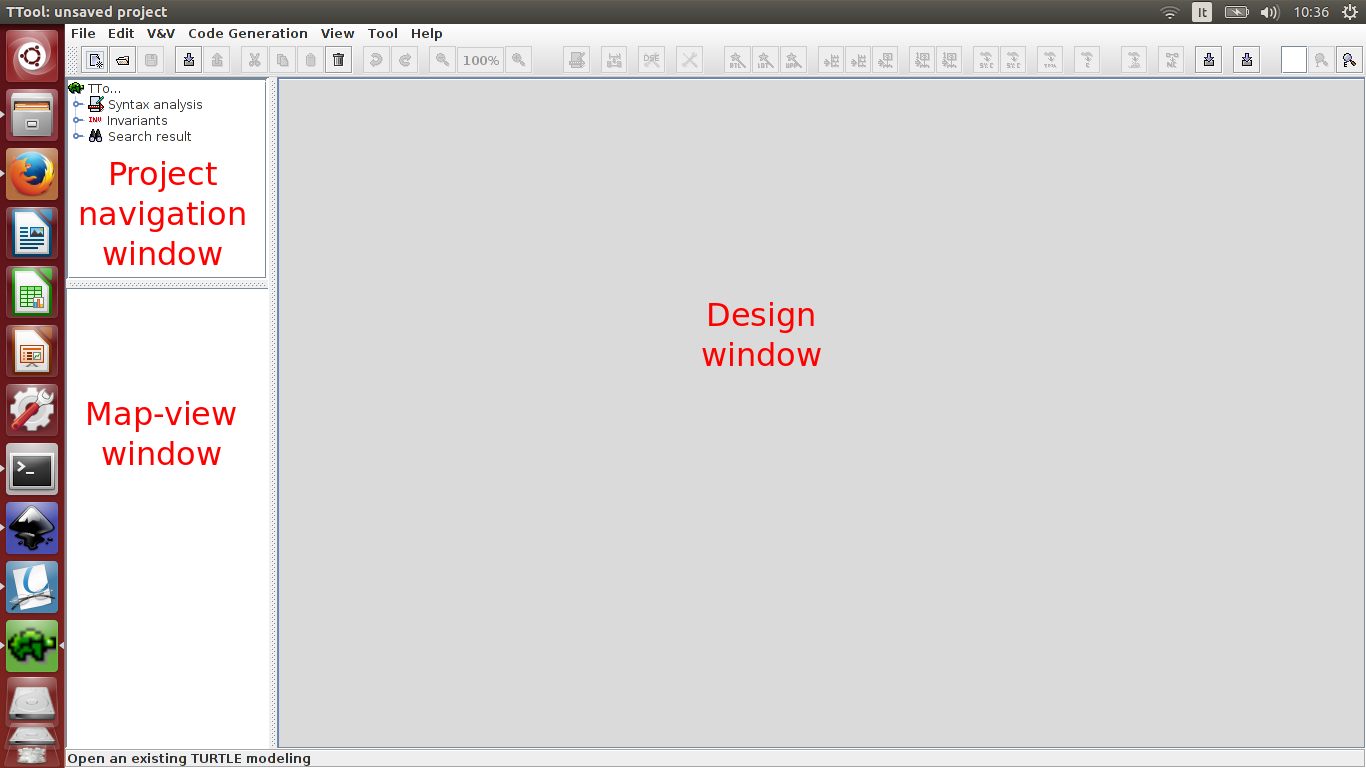
\includegraphics[width=\screenshotsize]{./figures/screenshot/NewPrj.png}
	\caption{The windows that compose a new project}
	\label{fig:NewPrj}
\end{figure}
%
\\Apart from the single application, communication, platform and mapping models (Fig.~\ref{fig:Tchart}) that compose a
design project, TTool/DIPLODOCUS also allows the creation of a Methodology diagram that represents the $\Psi$-chart
approach. To create such a Methodology diagram, right click in the Design window and select \texttt{New DIPLODOCUS
Methodology}, this will create the diagram shown in Fig.~\ref{fig:MethDiag}.
%
\begin{figure}[htbp]
	\centering
	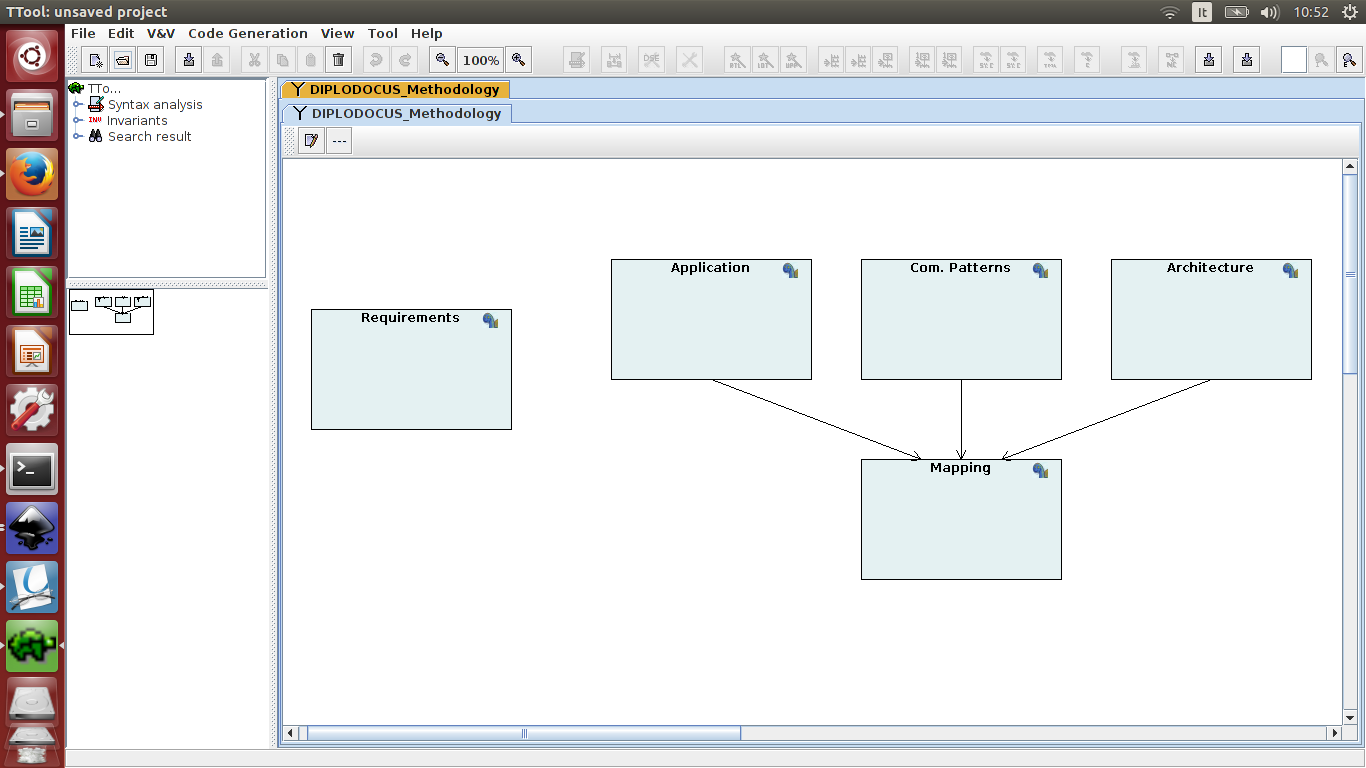
\includegraphics[width=\screenshotsize]{./figures/screenshot/MethDiag.png}
	\caption{The Methodology diagram of the $\Psi$-chart approach}
	\label{fig:MethDiag}
\end{figure}
%
For each box in Fig.~\ref{fig:MethDiag}, a reference to a diagram can be added by right-clicking on it and selecting
\texttt{Add diagram reference}. This opens a dedicated window such as the one in Fig.~\ref{fig:AddDiagRef}, where, for
instance, the references of up to 3 application diagrams can be added. After their addition, the Methodology diagram
appears as in Fig.~\ref{fig:RefDiagAdded}.
%
\begin{figure}[htbp]
	\centering
	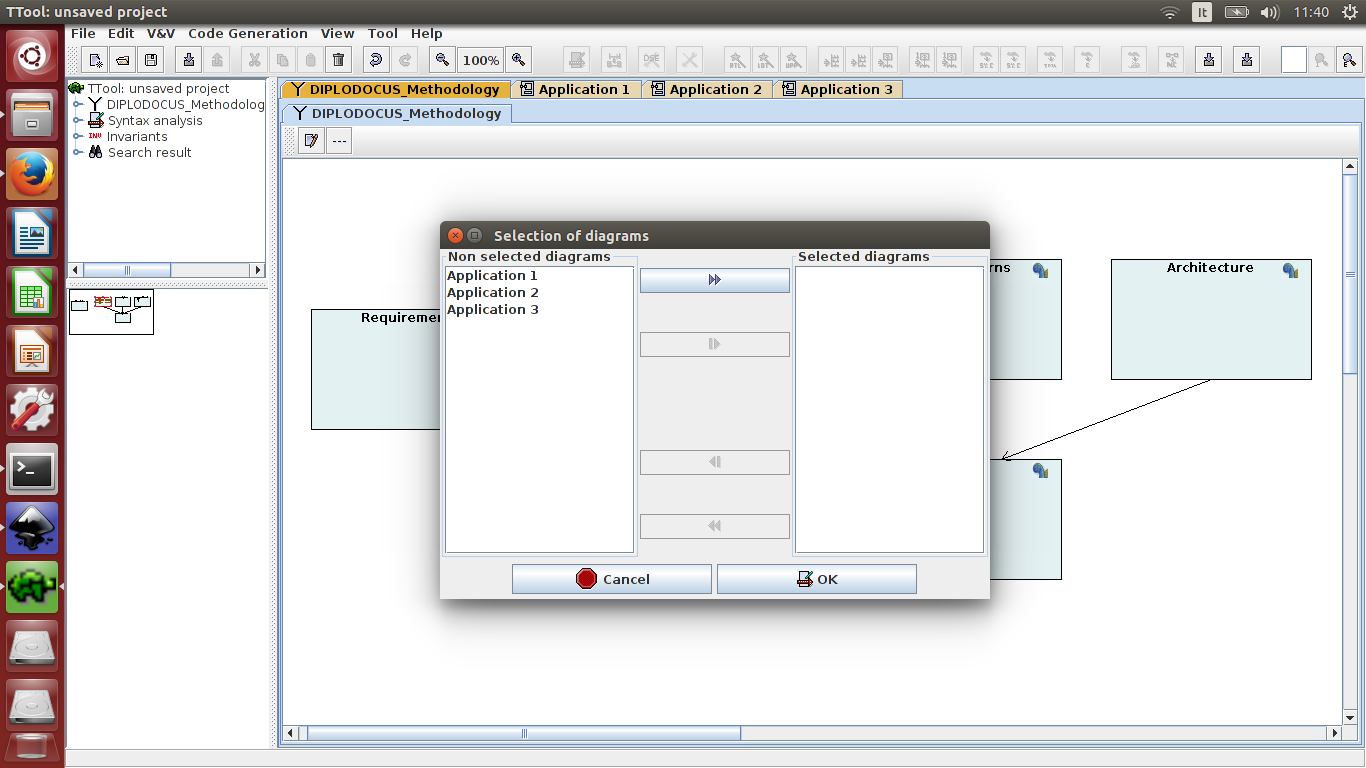
\includegraphics[width=\screenshotsize]{./figures/screenshot/AddRefDiag.png}
	\caption{The graphical window to add a reference to a diagram to the Methodology diagram}
	\label{fig:AddDiagRef}
\end{figure}
%
\begin{figure}[htbp]
	\centering
	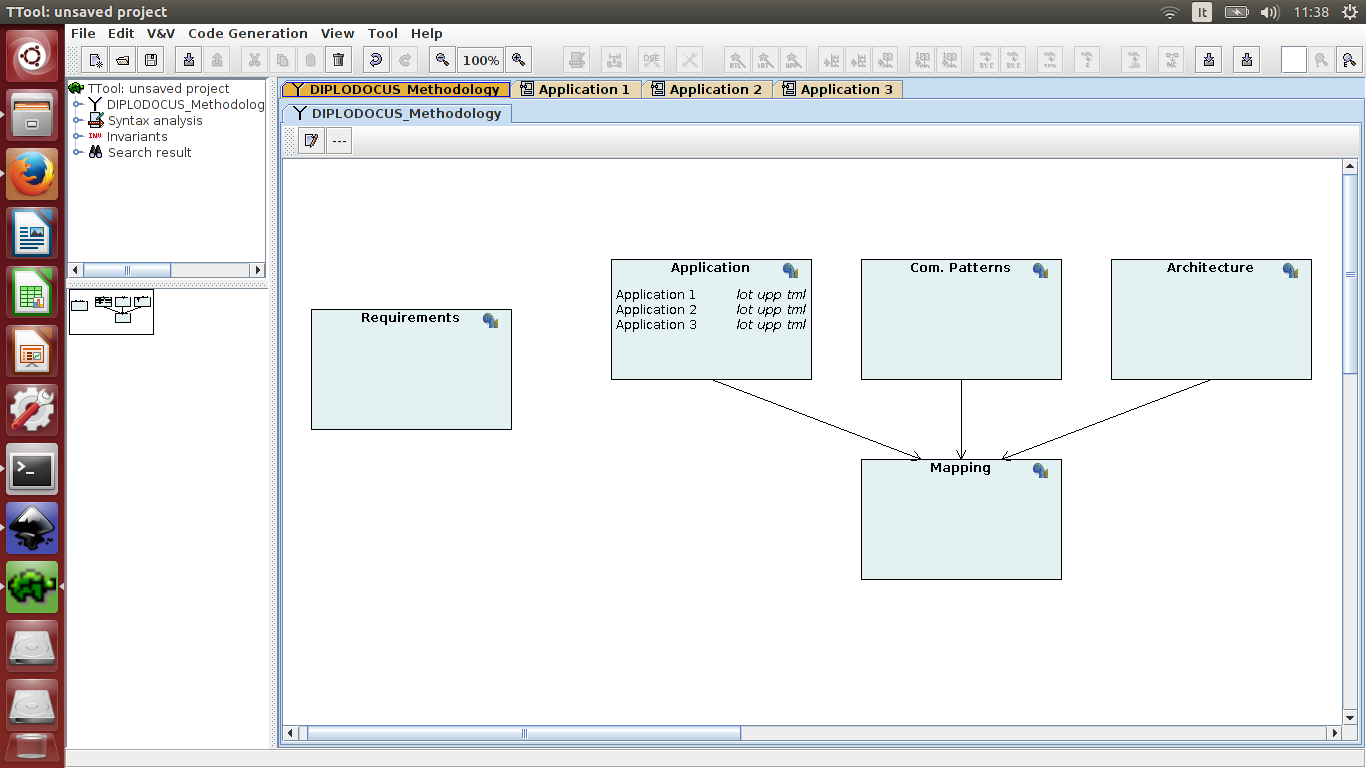
\includegraphics[width=1.0\textwidth]{./figures/screenshot/RefDiagAdded.png}
	\caption{The Methodology diagram after the introduction of 3 references to 3 different application diagrams}
	\label{fig:RefDiagAdded}
\end{figure}
%
\\With respect to the terminology used so far, before continuing the tutorial, we now distinguish between a
\textit{panel} and a \textit{diagram}. Generally speaking, a panel is a diagram container that can contain more than one
diagram. In Fig.~\ref{fig:PanelvsDiag}, we graphically show this difference with a screen capture of the complete ZigBee
design. The DIPLODOCUS\_Methodology panel can contain only one diagram, whereas panels for other models (application,
communication, mapping, platform) can contain more than one diagram.
%
\begin{figure}[htbp]
	\centering
	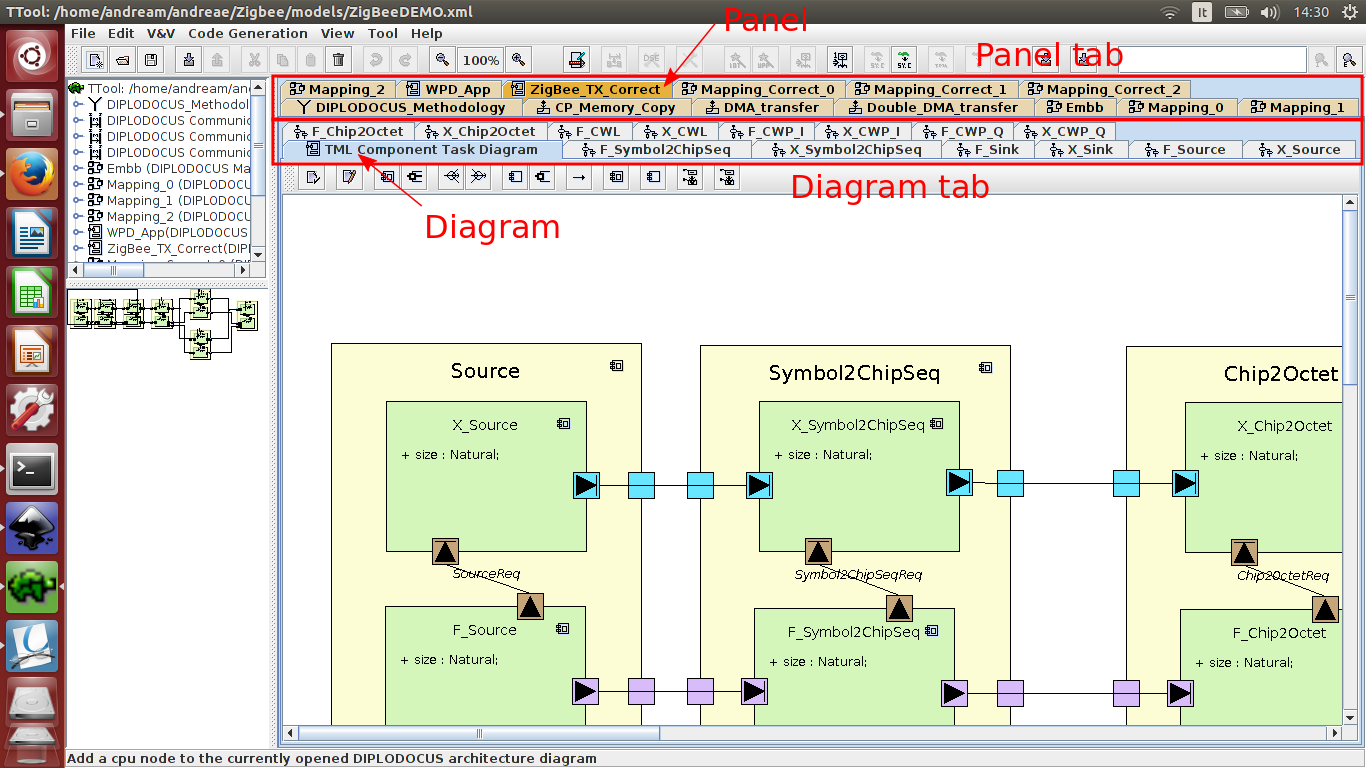
\includegraphics[width=\screenshotsize]{./figures/screenshot/PanelvsDiag.png}
	\caption{The difference between a panel and a diagram}
	\label{fig:PanelvsDiag}
\end{figure}
%
\\At this point we can save the project by clicking on the dedicated button, Fig.~\ref{fig:SaveButton} or by selecting
\texttt{File->Save as} from the main menu bar. We will name the project \texttt{ZigBeeTX} as shown in
Fig.~\ref{fig:SaveName} and save it in the folder that is purposed by default by the tool for all projects. This folder
is located in \texttt{your-home/TTool/modeling/}.
%
\begin{figure}[htbp]
	\centering
	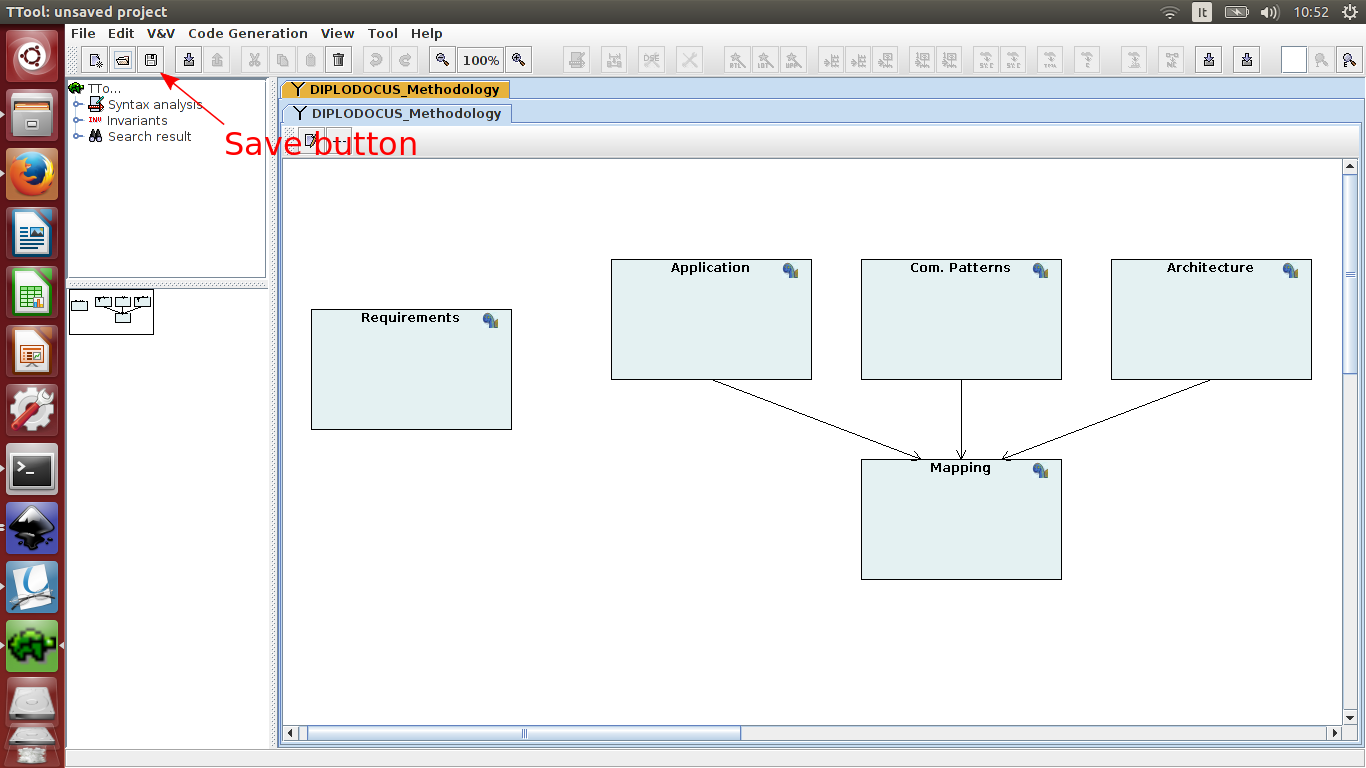
\includegraphics[width=\screenshotsize]{./figures/screenshot/SaveButton.png}
	\caption{The location of the \texttt{Save} button in the button bar}
	\label{fig:SaveButton}
\end{figure}
%
\begin{figure}[htbp]
	\centering
	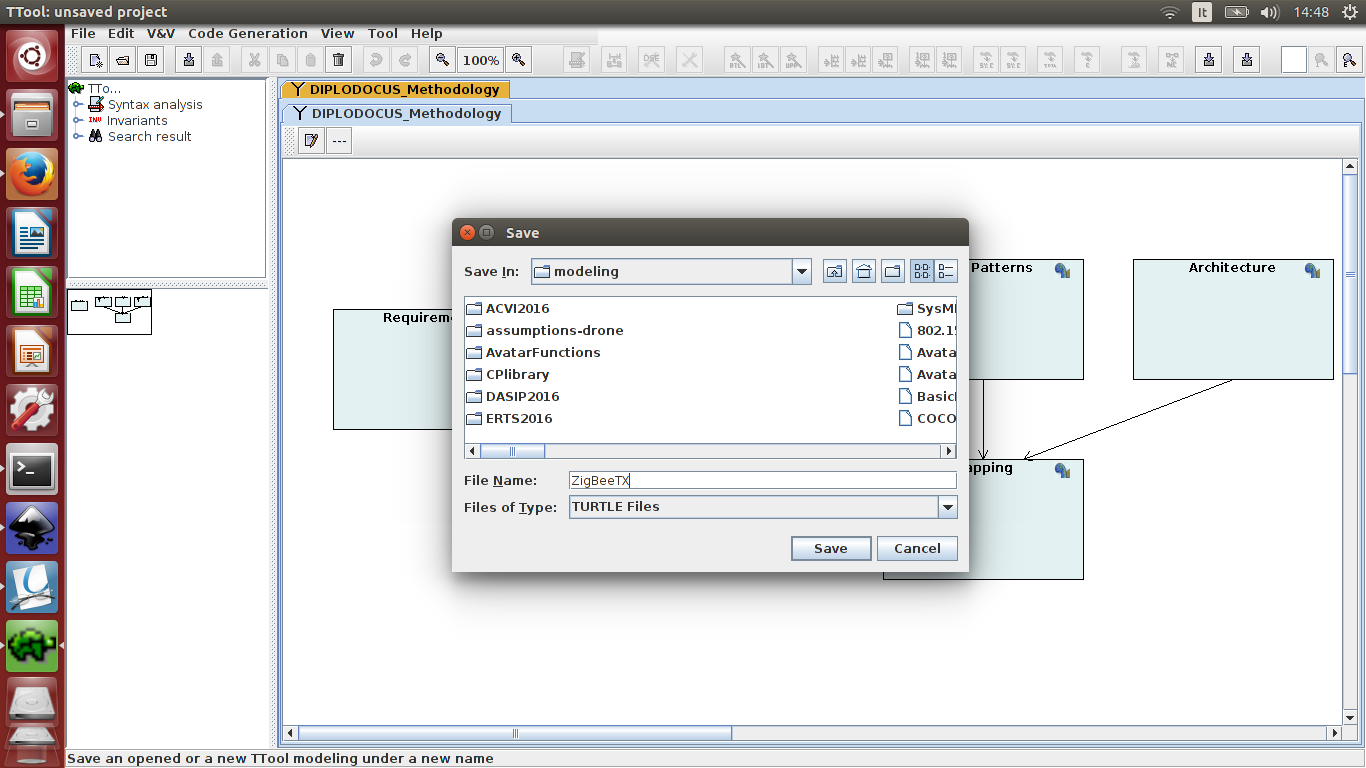
\includegraphics[width=\screenshotsize]{./figures/screenshot/SaveName.png}
	\caption{Saving the project of the ZigBee transmitter}
	\label{fig:SaveName}
\end{figure}
%
We now continue our tutorial with the description of the data-link layer of the ZigBee transmitter that we will design.
Each of the next sections is organized as follows: we will first introduce the reader to the theoretical aspects of the
design (e.g., what Zigbee is, the architecture of the platform that we target). Subsequently, we show the complete
diagrams that correspond to each part of the design or the tool windows that are used to perform a specific task (e.g.,
add a simulation breakpoint). We then illustrate to the reader how these diagrams can be created or these windows can be
used.
%
%
%
\newpage
\section{Modeling a ZigBee transmitter}
\label{sec:Modeling}
%
In this section we present the application, communication, platform and mapping models that we created specifically for
the design of the ZigBee transmitter. We use this case study as an example to demonstrate the modeling
facilities offered by TTool/DIPLODOCUS\footnote{Note that the complete model of
this tutorial is released with TTool and can be opened by clicking menu
\texttt{File>>Open} and then selecting file \texttt{ZigBeeTutorial.xml} under directory
\texttt{DIPLODOCUS} from the dialog box that opens.}
%
\subsection{The functionality of a ZigBee transmitter (data-link layer)}
%
Generally speaking, an application model (Fig.~\ref{fig:PsiChartApp}) captures the system's functionality (e.g., a
signal-processing or video-compression algorithm). This model must be created regardless of the resources that are
available for execution purposes (i.e., hardware and/or software resources) and must express all potential parallelism
between operations. This model must express both the processing of information (e.g., computations) and the dependencies
(e.g., communications) between these processing operations.
%
\begin{figure}[htbp]
	\centering
	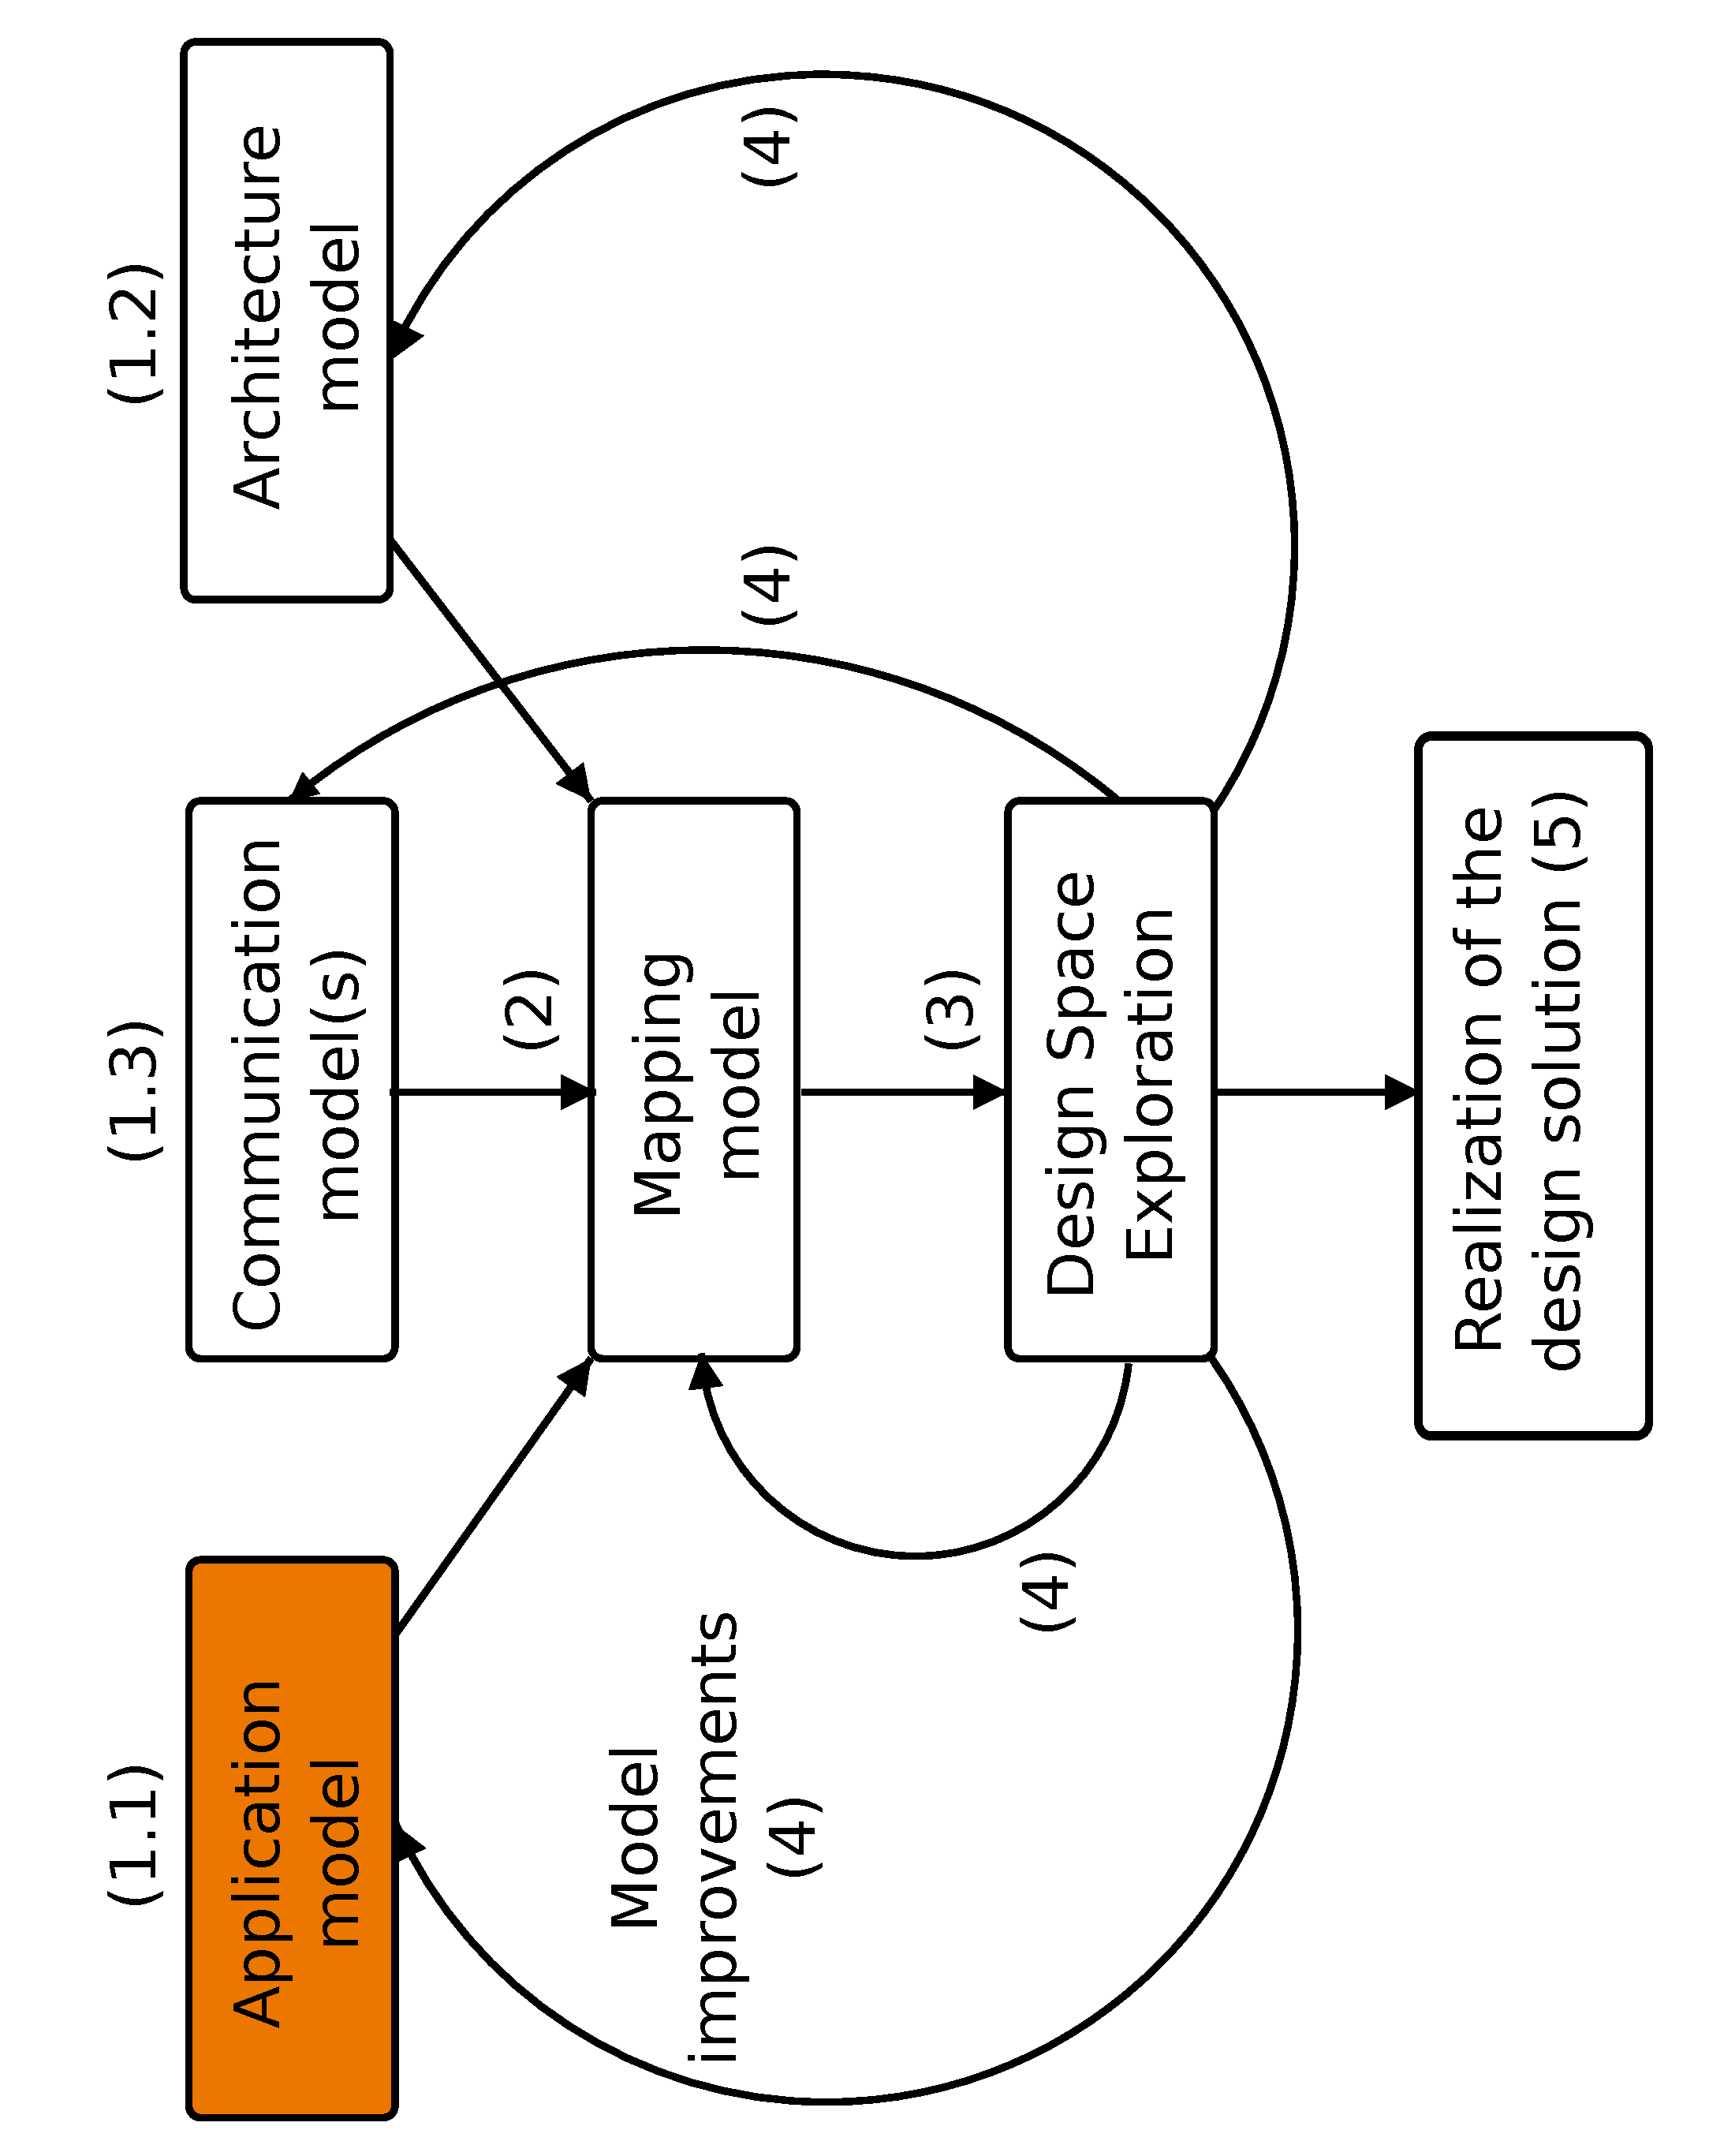
\includegraphics[angle=-90,origin=c,width=0.4\textwidth]{figures/PsiChartApp.pdf}
	\caption{The step of application modeling, that is described in this section, in the context of the $\Psi$-chart
    design approach}
	\label{fig:PsiChartApp}
\end{figure}
%
\\In this subsection we describe the application model for the data-link layer of a ZigBee transmitter. The ZigBee
protocol is issued by the IEEE 802.15.4 standard that specifies both the MAC and the PHY layers of the IEEE 802.15.4
protocol. It is a standard for low-rate Wireless Personal Area Networks (WPANs), which are used to convey information
over relatively short distances. ZigBee has been deployed for several applications including Wireless Sensor Networks
(WSN) for building automation, remote control, health care, smart energy, telecommunication services. Among the
different schemes that can be derived from the IEEE 802.15.4 standard for a ZigBee transmitter, we selected the one
proposed by~\cite{Koteng06}, shown in Fig.~\ref{fig:TXBlockDiag}, because of its simplicity in terms of implementation.
%
\begin{figure}[!htbp]
	\centering
	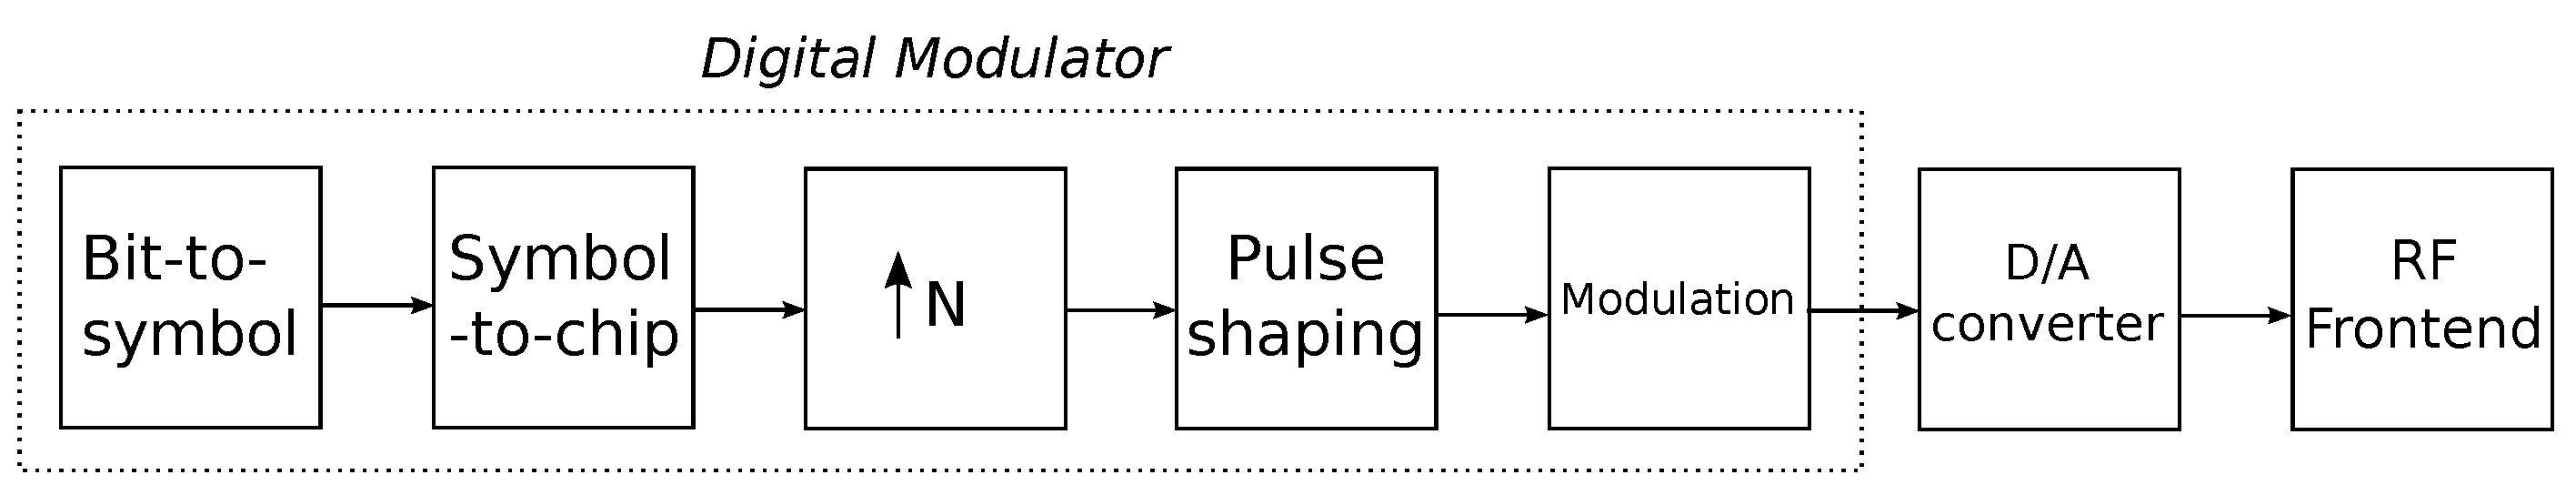
\includegraphics[width=0.8\textwidth]{figures/TXBlockDiagram.pdf}
  	\caption{The functional block diagram of the ZigBee transmitter as proposed by~\cite{Koteng06}.}
	\label{fig:TXBlockDiag}
\end{figure}
%
\\Fig.~\ref{fig:ZigBeeTX} shows the TTool/DIPLODOCUS diagram corresponding to the data-flow model of
Fig.~\ref{fig:TXBlockDiag} implemented for EMBB. This means that the diagram of Fig.~\ref{fig:ZigBeeTX} expresses the
functionality of the algorithm in Fig.~\ref{fig:TXBlockDiag}, according to the signal-processing operations available in
the platform EMBB (see sub-section~\ref{subsec:Embb}). This statement may apparently contradict the above claim that
a system's functionality and its resources are modeled separately. However, the reader must keep in mind that the
functionality of a system (the ZigBee transmitter, in our case) can, and must, be modeled independently of the specific
resources of a target platform (the processors, buses and memories of EMBB, in our case). On the contrary, it cannot be
modeled independently of the services offered by these resources (the signal-processing operations offered by these
processors, in our case). Frequently, these services, do not correspond to the mathematical operations of
signal-processing algorithms, such as the one in Fig.~\ref{fig:TXBlockDiag}.\\
%
In Fig.~\ref{fig:ZigBeeTX}, the block labeled Source produces the data to be transmitted in the form of a flow of bits.
These data are then converted to symbols by the Symbol2ChipSeq block. In this block, we model the mapping of each
incoming 4-bits symbol to one of the 16 sequences of 32 chips as defined by the IEEE standard 802.15.4. The
Chip\_to\_Octet block then transforms each incoming chip (bit) of a chip sequence into an unsigned 8-bits integer as
expressed in equation~\ref{eq:INTL}:
%
\begin{equation}
\label{eq:INTL}
\{\texttt{0}; \texttt{1}\} \rightarrow \{\texttt{0x00}; \texttt{0x01}\}
\end{equation}
%
Chip\_to\_Octet also separates the even-indexed chips that are used to modulate the in-phase (I branch) carrier
component from the odd-indexed chips that are used to modulate the quadrature (Q branch) carrier component. The output
is then transformed by means of a Component Wise Lookup (CWL block) that maps unsigned 8-bits integers to signed 16 bits
integers as expressed by equation~\ref{eq:CWL}:
%
\begin{equation}
\label{eq:CWL}
\{\texttt{0x00}; \texttt{0x01}\} \rightarrow \{\texttt{0xffff}; \texttt{0x0001}\}
\end{equation}
%
At this point, given the separation of the I and Q branches, their pulse shaping can be executed independently. The
application graph exposes this parallelism by forking the output data of block CWL to two distinct Component Wise
Product (CWP) blocks, CWP\_I for the I branch and CWP\_Q for the Q branch. These blocks multiply the input samples with
a half-sine wave to realize the O-QPSK modulation. The quadrature shift between the I and Q branches is implemented by
means of an offset between the memory addresses of the output samples. This
results into a frame of complex samples (16 bits for the real part and 16 bits for the imaginary part) that is then collected by block Sink and transmitted over the
air.\\
%
Each block of the model in Fig.~\ref{fig:ZigBeeTX} is composed of two sub-blocks (tasks): one modeling the
data-processing and one modeling the related control operations. By convention
we name the data-processing tasks with a heading X that stands for eXecution and the control tasks with a heading F that stands for Firing.
%
\begin{figure}[!htbp]
	\centering
	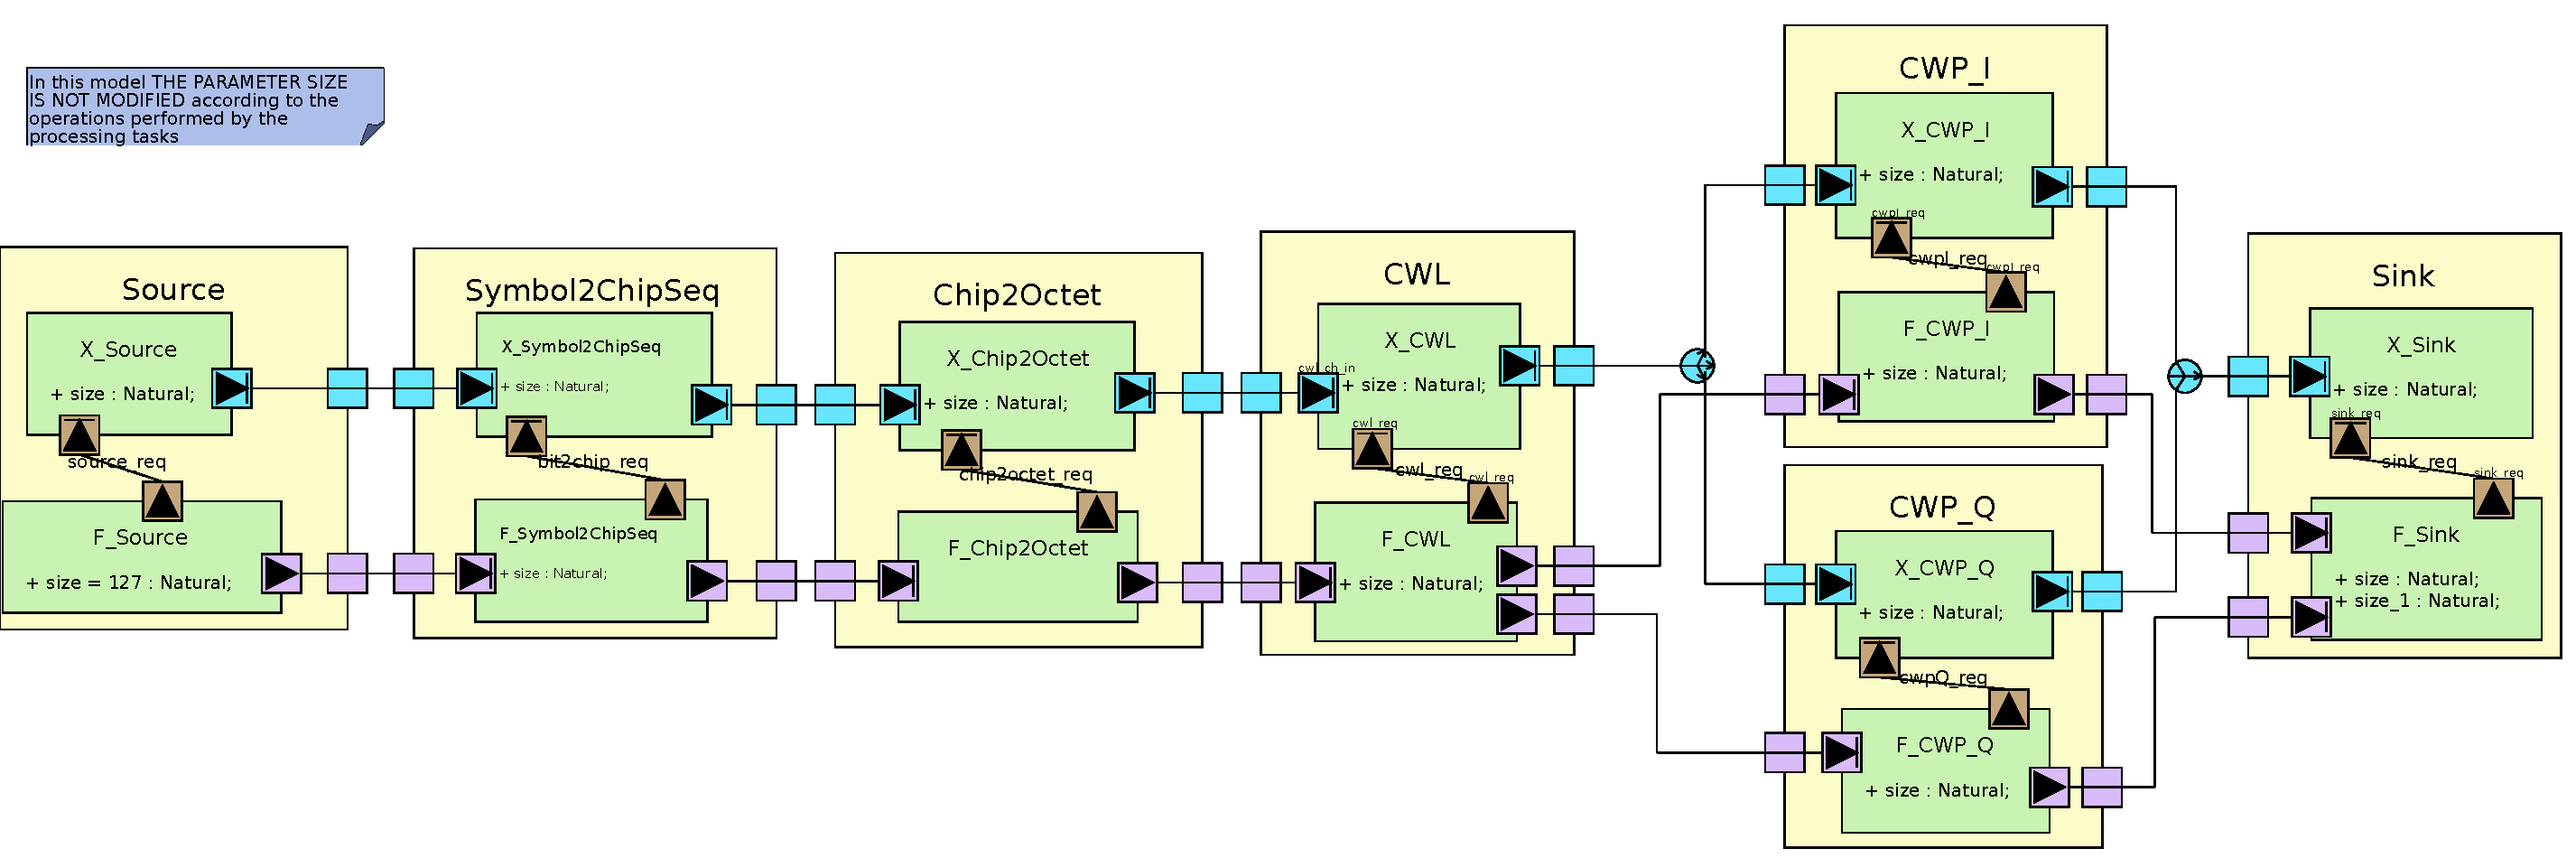
\includegraphics[width=\textwidth]{figures/ZigbeeApp.pdf}
	\caption{The TTool/DIPLODOCUS model of the ZigBee transmitter}
	\label{fig:ZigBeeTX}
\end{figure}
%
\subsection{Creating the application model of a ZigBee transmitter (data-link
layer)}
%
Let's now reload the ZigBee project that we have created in Section~\ref{sec:Project}. This can be done by clicking on
the dedicated button, Fig.~\ref{fig:Open}, or by selecting \texttt{File->Open}.
%
\begin{figure}[!htbp]
	\centering
	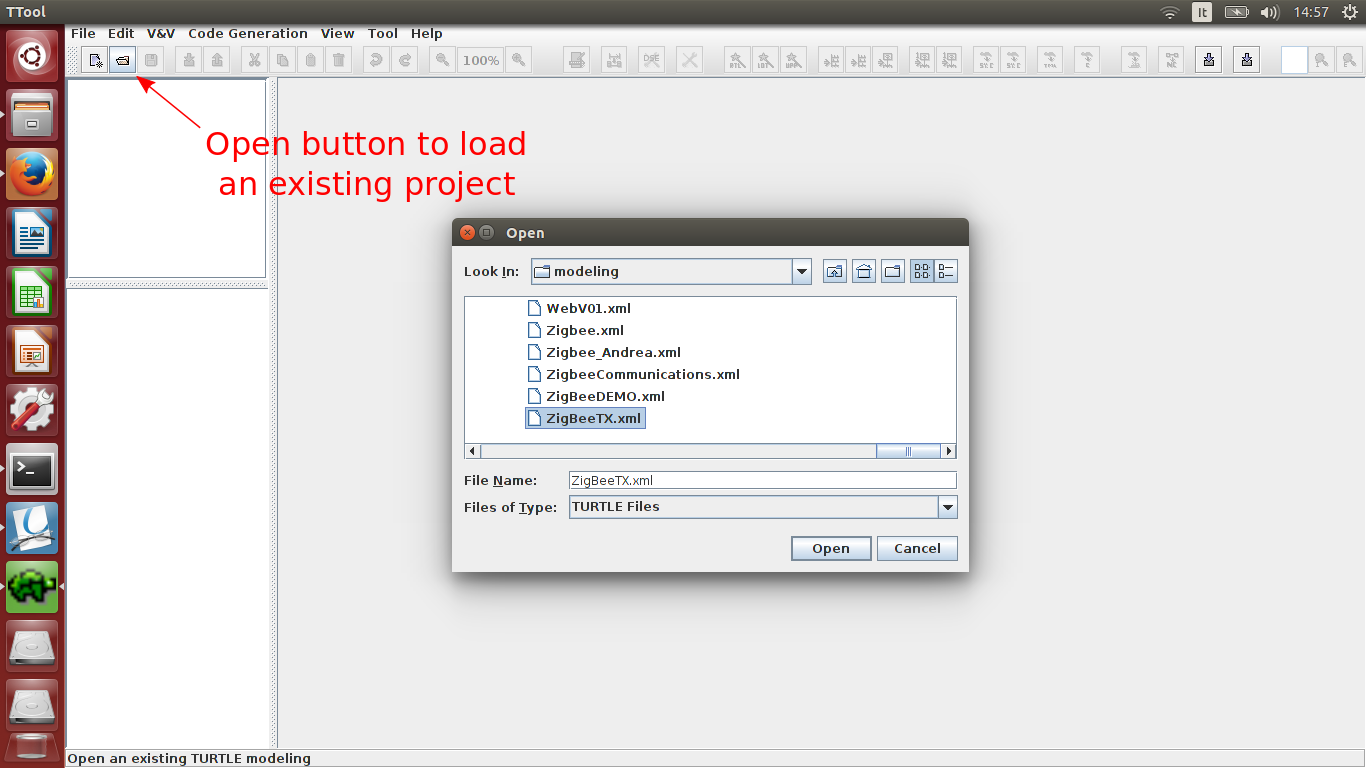
\includegraphics[width=\screenshotsize]{figures/screenshot/Open.png}
	\caption{The location of the \texttt{Open} button in the button bar}
	\label{fig:Open}
\end{figure}
%
\\To create the application model in Fig.~\ref{fig:ZigBeeTX}, we first need to create an application panel and
then start adding the related diagrams. For this purpose, let's right click in the panel tab and select \texttt{New
Partitioning - Functional view}. The tool will create a panel that contains a
sub-panel where the user can draw the SysML Block Definition diagram that captures the structure of the system's functionality, Fig.~\ref{fig:AppPanel}, in
terms of interconnected blocks. The default name of this sub-panel is \texttt{TML Component Task Diagram}. As introduced
in Section~\ref{sec:Introduction}, TML stands for Task Modeling Language. It is a textual language, alternative to the
graphical description provided by UML/SysML diagrams. In this version of the tutorial, we do not cover the syntax and
semantics of the language. Some of the TML syntax and semantics is covered in~\cite{Waseem09} and in\cite{EnriciThesis}.
%
\begin{figure}[!htbp]
	\centering
	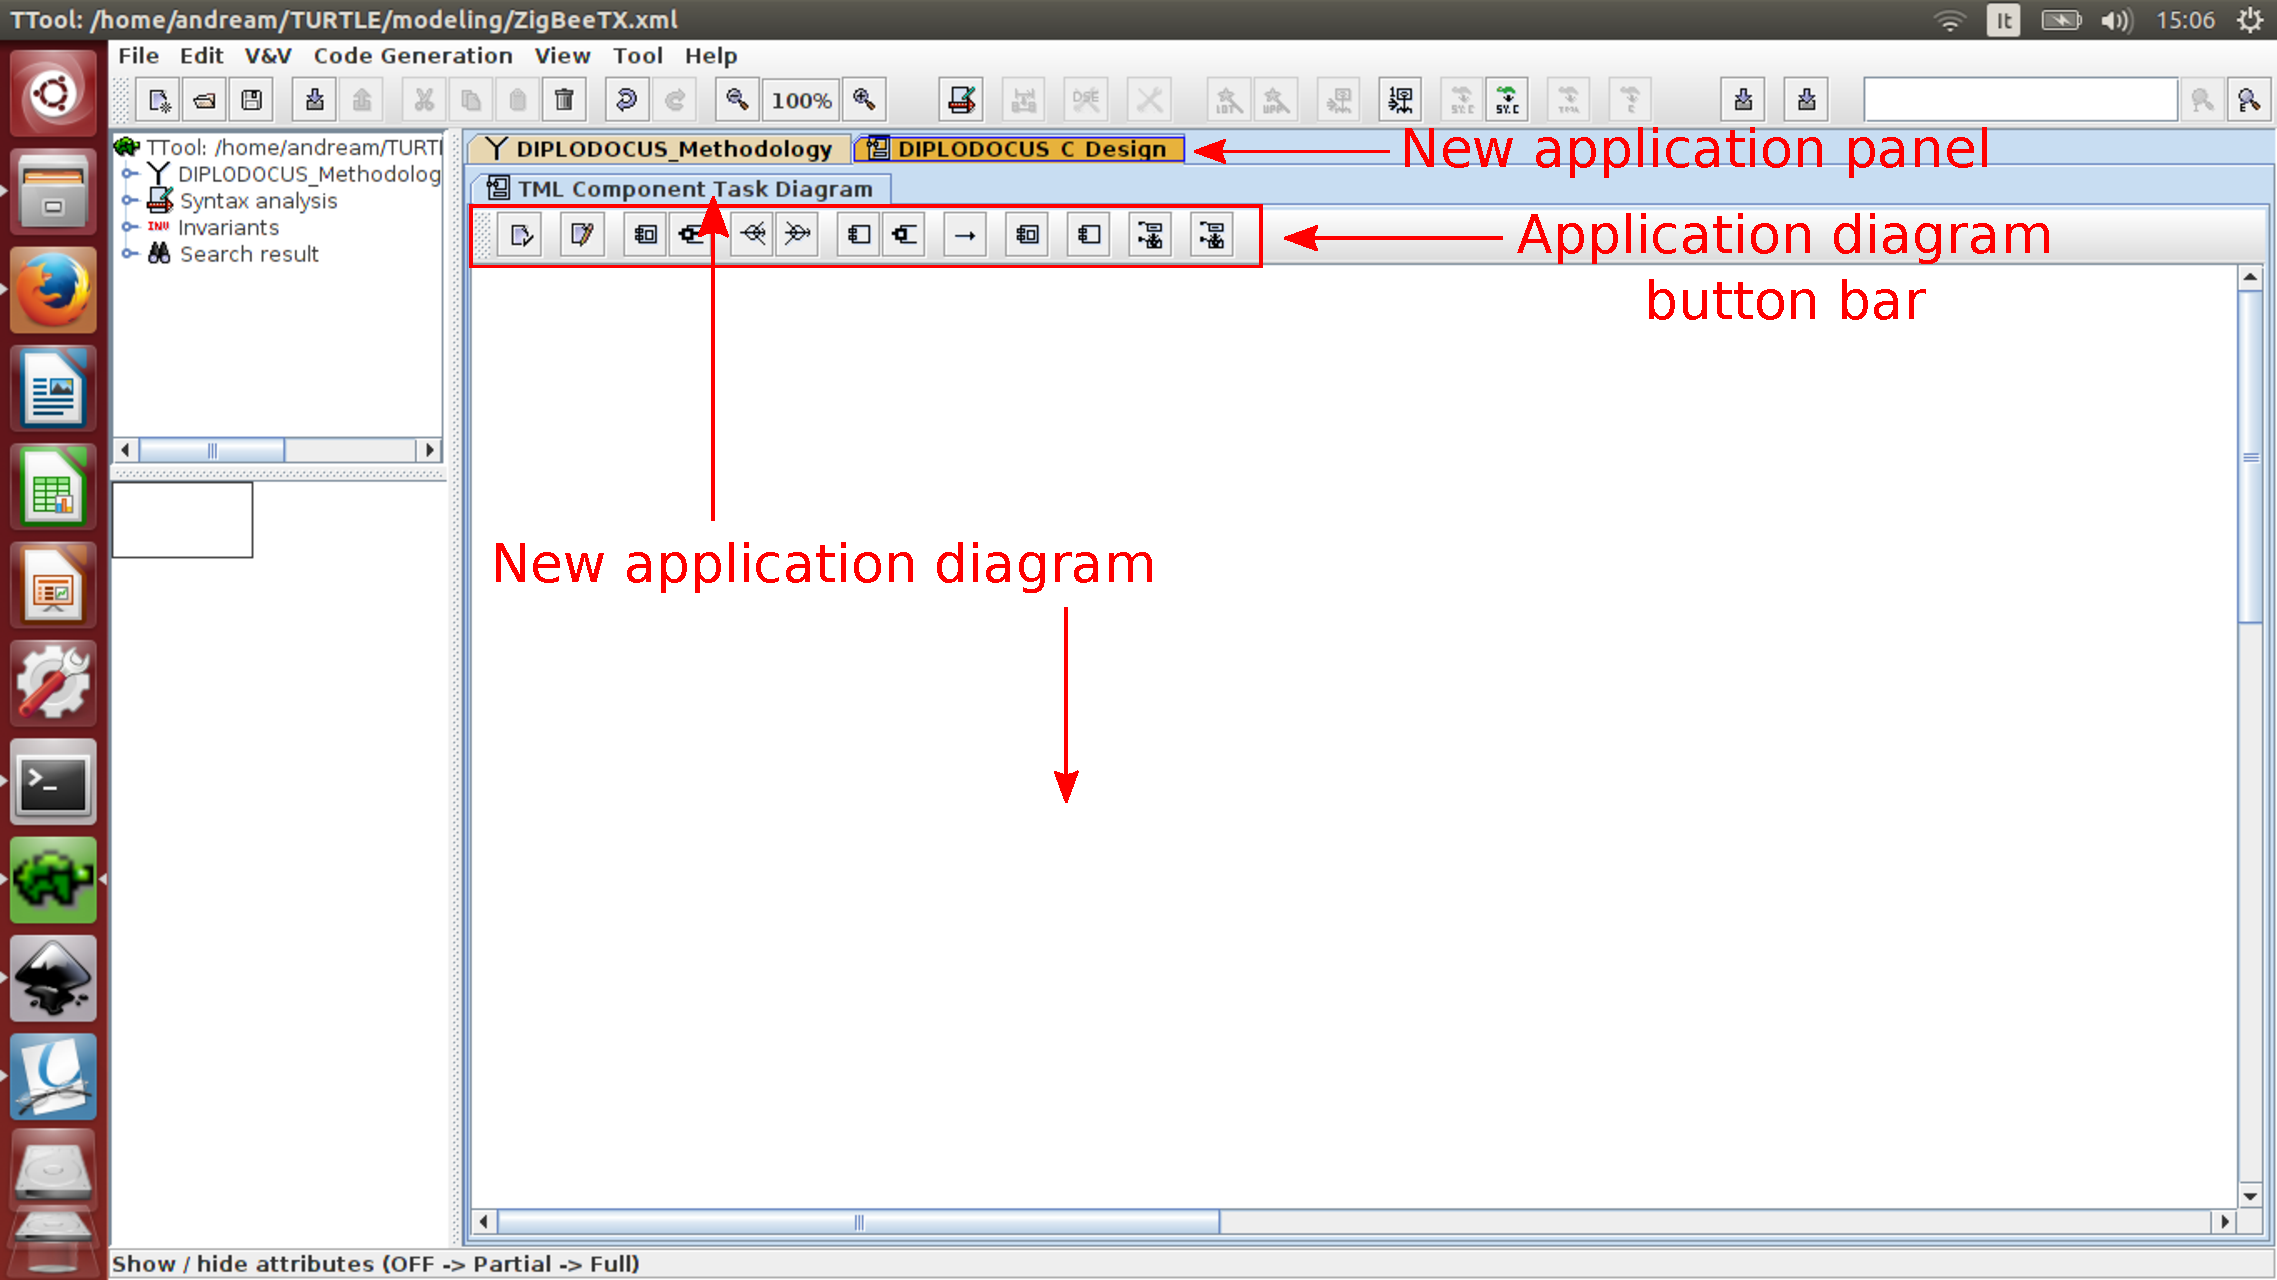
\includegraphics[width=\screenshotsize]{figures/screenshot/AppPanel.pdf}
	\caption{The creation of a new application panel and diagram}
	\label{fig:AppPanel}
\end{figure}
%
\\To rename the application panel (we suggest that you rename it \texttt{ZigBeeApp}), right-click on the panel and select
\texttt{Rename}. Let's now start to build the application model of the data-link layer ZigBee transmitter! There are
many approaches that can be taken to express the mathematical algorithm in Fig.~\ref{fig:TXBlockDiag} in a set of
connected data-processing and control operations. The approach that we used, resulting in the diagram in
Fig.~\ref{fig:ZigBeeTX}, is to separate the data-processing operations and the control operations in independent blocks
(\textit{primitive components} in the language of DIPLODOCUS). Another approach would be to use only a single primitive
component to represent both data-processing and control aspects. However, this modeling approach would result in several
issues at the mapping step. In fact, the architecture of EMBB separates the control part from the data-processing in
physically distinct units. Instead, for each of the signal-processing instructions that are available in EMBB, we
instantiate a \textit{composite component} that contains two primitive components. The latter are named with the prefix
\texttt{X\_} (eXecution) for the data-processing part and with the prefix \texttt{F\_} (Firing) for the control part.
In the frame of this modeling approach, execution of the \texttt{X\_} component is triggered by the \texttt{F\_}
component.\\
%
An application model in TTool/DIPLODOCUS must always include a \textit{Source} and a \textit{Sink} components. The
Source component emits the data to process and the related control information. The Sink component, instead, collects
both data and control items. To draw the Source component as in Fig.~\ref{fig:ZigBeeTX}, left-click on the \texttt{Add
a composite component} button in the \texttt{TML Composite Task Diagram} panel. Then left-click in the design area where
you want the composite component to be placed, Fig.~\ref{fig:Src1}. Double-click on the component and re-name it as
\texttt{Source}. Enlarge the composite component, then instantiate two primitive components, one for the data part
(eXecution) and one for the control part (Firing), by left-clicking on the \texttt{Add a primitive component} button.
Place the two primitive components within the composite component.
%
\begin{figure}[!htbp]
	\centering
	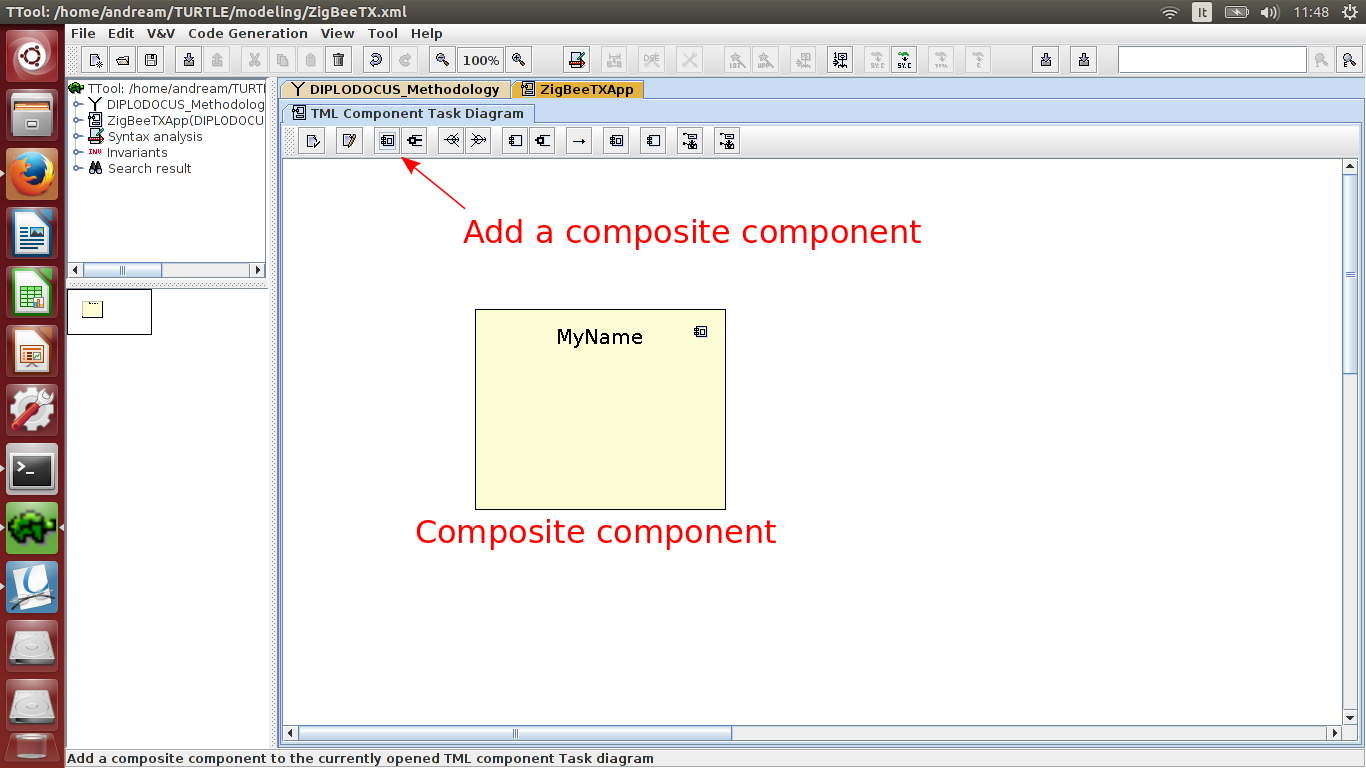
\includegraphics[width=\screenshotsize]{figures/screenshot/Src1.png}
	\caption{The instantiation of the \texttt{Source} composite component}
	\label{fig:Src1}
\end{figure}
%
%\begin{figure}[!htbp]
%	\centering
%	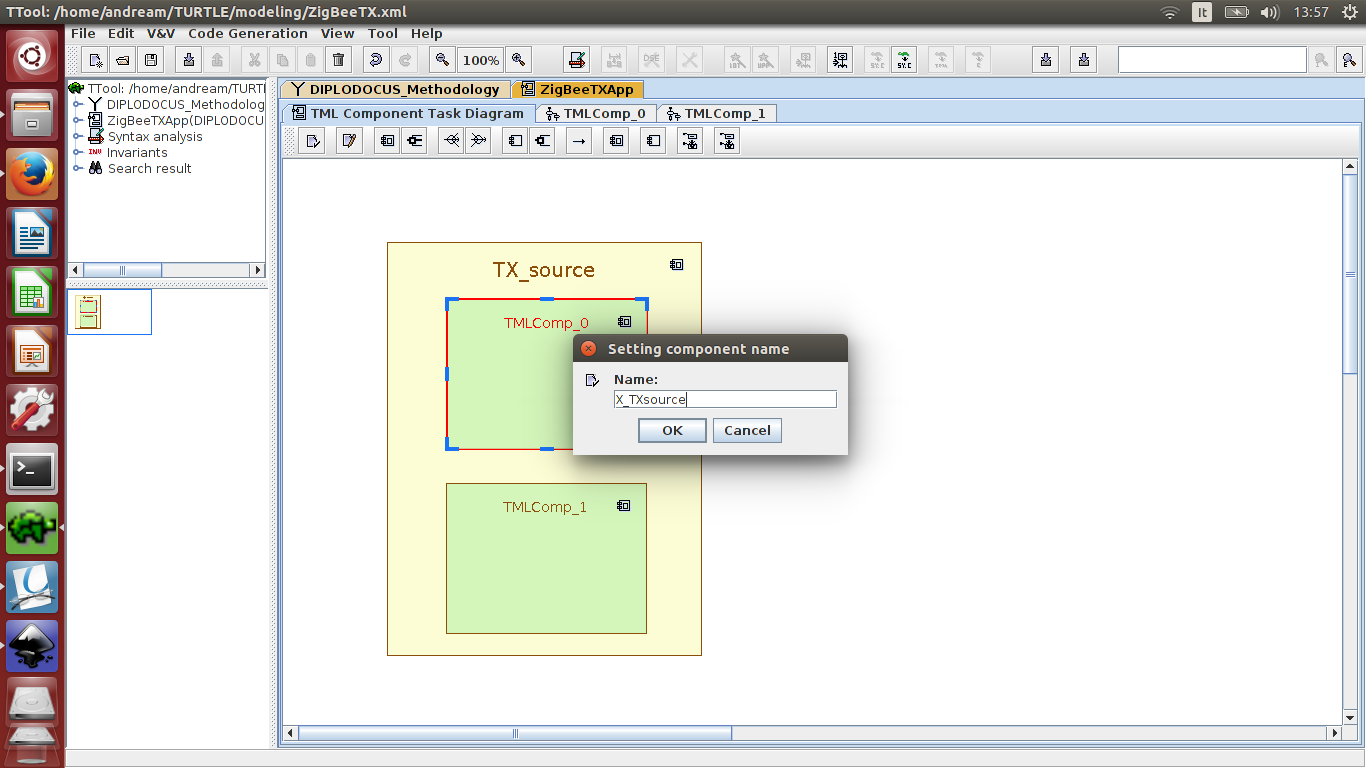
\includegraphics[width=0.7\textwidth]{figures/screenshot/Src2.png}
%	\caption{The instantiation of the \texttt{Source} primitive components}
%	\label{fig:Src2}
%\end{figure}
%
The primitive components are automatically attached to the composite component (i.e., they cannot be moved outside of
the composite component). Rename the primitive components as \texttt{X\_source} and \texttt{F\_source} by
double-clicking on the the component's default name, then type the new name. Please notice that two new tabs appear on
the right-hand side of tab \texttt{TML Component Task Diagram}. We will use these tabs later on in this tutorial to
design the activity diagram internal to each primitive component.\\
%
\subsubsection{Attributes of a primitive component}
%
While composite components are simply containers for primitive components, the latter have attributes and contain a
SysML Activity Diagram. One parameter that must be specified for this design is
the number of data samples that our model will process (\texttt{size}). Control
variables or attributes such as \texttt{size} are used by the control-flow operators of an activity diagram. Therefore, for each \texttt{F\_} primitive component that uses \texttt{size}, we must
declare such a control variable. This is done by double-clicking in the green area of a primitive component, as shown in
Fig.~\ref{fig:Src3}.
%
\begin{figure}[!htbp]
	\centering
	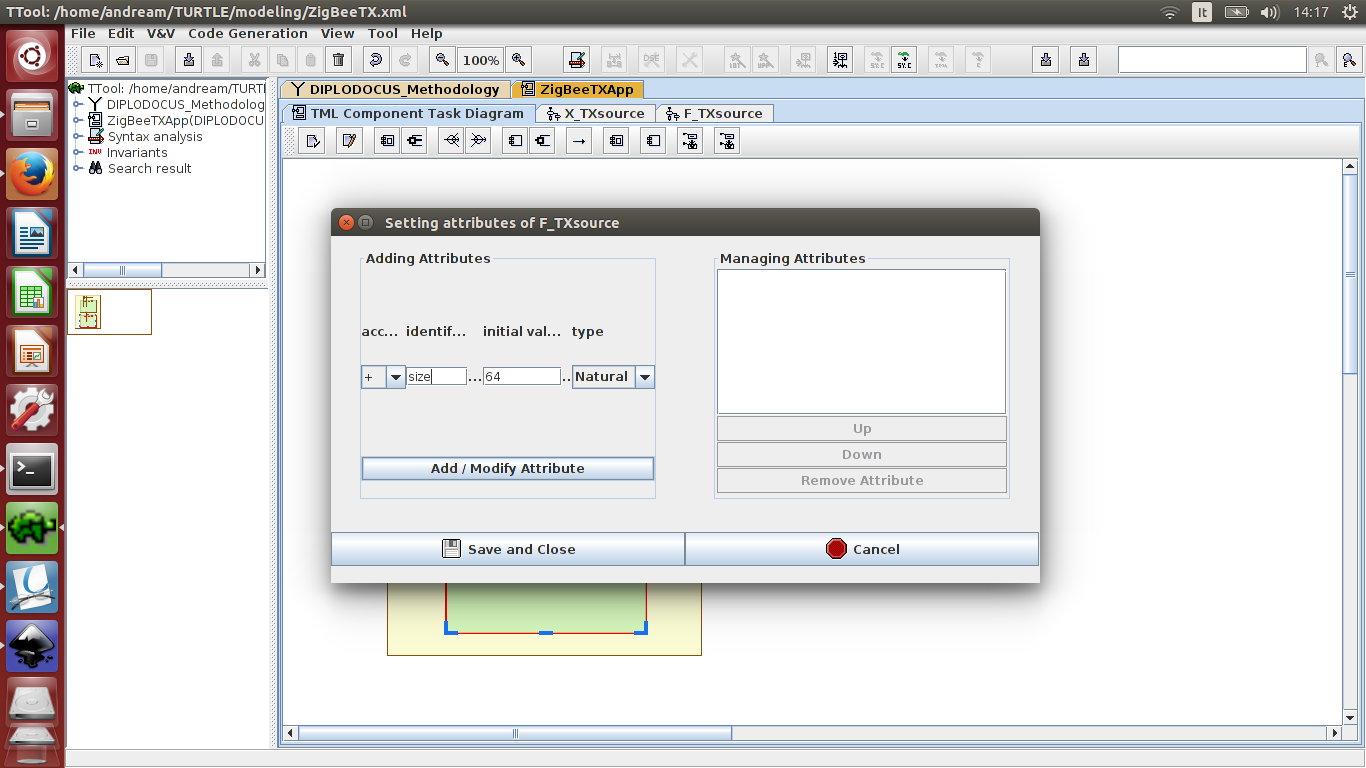
\includegraphics[width=\screenshotsize]{figures/screenshot/Src3.png}
	\caption{The creation of the control parameter \texttt{size}}
	\label{fig:Src3}
\end{figure}
%
We define the parameter \texttt{size} as of type natural and assign it the default value of 31 as in this case study we
analyze the transmission of a ZigBee packet that is composed of 25 bytes payload and 6 bytes header. Then, click on the
\texttt{ADD/Modify attribute} button. Clicking on the \texttt{Save and Close} button will add the variable to the
primitive component that will list it in its green area. The parameter \texttt{size} must be created for both X\_source
and F\_source primitive components, but for the X\_source component, it is not necessary to specify a default value (to
define the control attribute) as it will be transmitted by F\_source. For component X\_source, we only need to declare
\texttt{size}. The scope of an attribute is local to the diagram of a primitive component. So far, it is not possible to
define or declare global attributes. The value of an attribute can be modified in a primitive component's diagram.
Additionally, the value of an attribute can be exchanged among primitive components as described in the next paragraph.
%
\subsubsection{Ports, channels, events and requests}
%
In TTool/DIPLODOCUS components communicate via channels, events and requests. More in detail, channels are used to
exchange data, whereas events and requests are used to exchange control information. Events are used to synchronize
control-flows, whereas requests are used to spawn the execution of primitive components. These three types of
communications are attached to components via ports. Two types of ports exist: composite ports for composite components
and primitive ports for primitive components.\\
%
Channels are characterized by a point to point communication between 2 tasks\footnote{A task is a primitive component in
the terminology of the TML language}. The possible types for a channel are: 
%
\begin{itemize}
    %
    \item Blocking Read - Non Blocking Write (BR-NBW): the emitter task can write infinite times while the receiver task
        blocks when attempting to read from an empty channel. Data are read in a FIFO. Therefore a BR-NBW channel is
        equivalent to an infinite FIFO buffer.
    \item Non Blocking Read - Non Blocking Write (NBR-NBW): the emitter task can write infinite times and the receiver
        task never blocks when attempting to read from an empty channel. A NBR-NBW channel is equivalent to a shared
        memory of infinite size between emitter and receiver.
    \item Blocking Read - Blocking Write (BR-BW): the emitter task blocks when attempting to write to a full channel and
        the receiver task blocks when attempting to read from an empty one. A BR-BW channel therefore is equivalent to a
        finite FIFO buffer.
    %
\end{itemize}
%
When configuring a port to be for a data channel, the user must specify the number of data samples (to be written or
read), and the maximum number of samples to be written before blocking (this second one for BR-BW only).\\
%
Events are characterized by a point to point asynchronous unidirectional communication between two tasks. Multiple
events arriving at the same task at a given moment are managed using a FIFO, which can be finite or infinite.
%
\begin{itemize}
    %
    \item In the case of infinite FIFO, events are never lost.
    %
    \item When using a finite FIFO, events arriving at the FIFO are stored in it. Two semantics are defined for finite FIFO:
    %
    \begin{itemize}
        %
        \item When the FIFO is full, the first (oldest) element is removed to leave space for the new one that is
            added.
        %
        \item When the FIFO is full, no event may be added: the event sender is blocked until the FIFO is not full.
        %
    \end{itemize}
    %
    \item In the case of a single element FIFO, with first event removal, it is equivalent to a hardware interrupt or a Unix signal.\\
    %
\end{itemize}
%
Up to five optional parameters can be specified for an event, and they can be Integer or Boolean. The Boolean type is
defined as an Integer, where the integer value '0' means false, while any other integer value means true.\\
%
Requests are characterized by a multipoint to one point asynchronous unidirectional communication between two tasks.
Multiple requests arriving to one task at a given moment are stored in an infinite FIFO (a FIFO is defined for each
destination task). They can be executed straight or after the previously stored
requests have been executed. In any case, since the FIFO is infinite, requests
are never lost.
Requests are never blocking for the sender task. Up to five optional parameters can be specified for a request, and they can be Integer or Boolean.\\
%

As the component in Fig.~\ref{fig:Src3} is the source of our design, we only need to add output ports. In this case, the
two primitive components have each one output flow: one to send data and one to send control information. Therefore, we
need to instantiate 2 primitive ports and 2 composite ports as in Fig.~\ref{fig:Ports1} and Fig.~\ref{fig:Ports2}. To
add a composite port to your design, left-click on the \texttt{Add a composite port} button and then place the port
anywhere within the boundaries of the composite component, it will be automatically attached to its edges. Then drag the
port on the right-hand side of the component as in Fig.~\ref{fig:Ports1}.
%
\begin{figure}[!htbp]
	\centering
	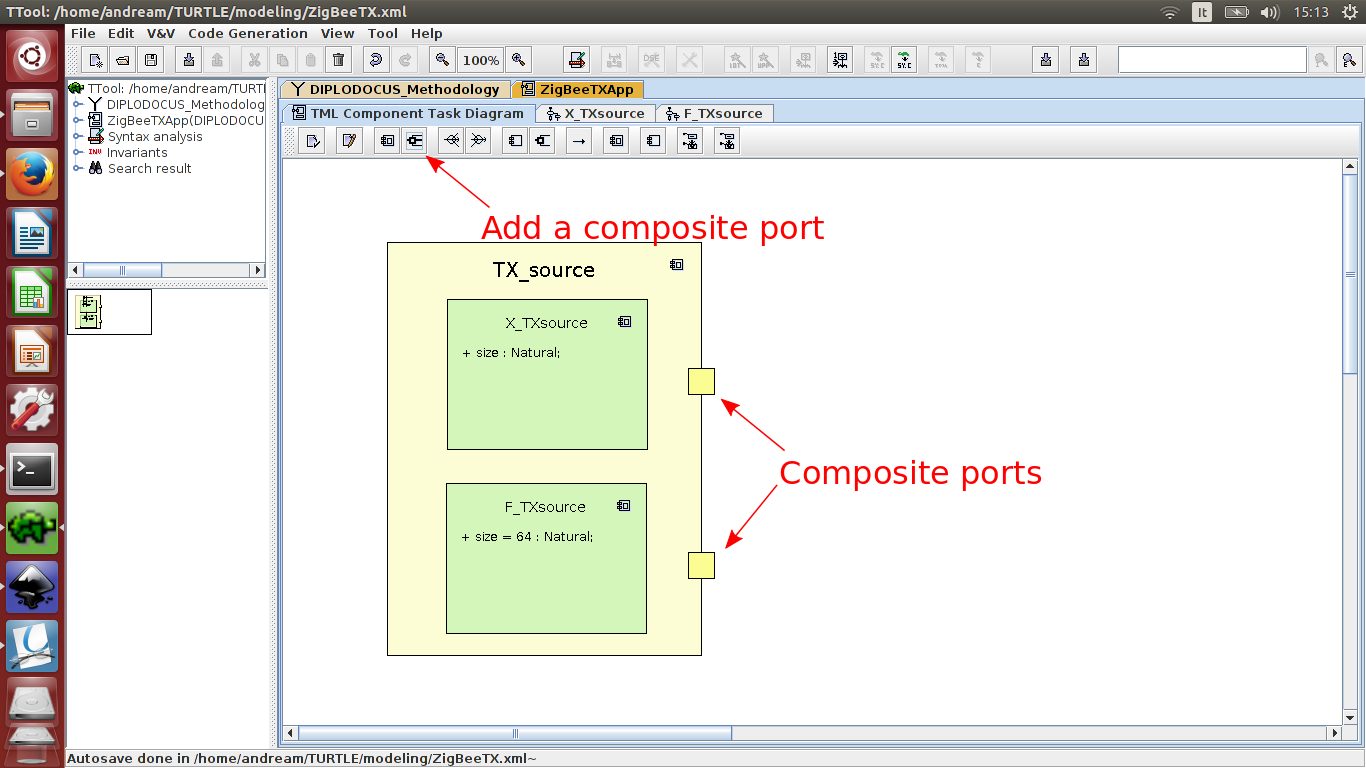
\includegraphics[width=\screenshotsize]{figures/screenshot/Ports1.png}
	\caption{The instantiation of composite ports to the composite component \texttt{Source}}
	\label{fig:Ports1}
\end{figure}
%
To add a primitive port, left-click on the \texttt{Add a primitive port} button and then place the port anywhere within
the boundaries of the primitive component, it will be automatically attached to its edges. Then drag the port on the
right-hand side of the component as in Fig.~\ref{fig:Ports2}. By default a port is instantiated as a channel port (blue
port) and is configured as an output port (rightward black arrow-head). The tool diplays the name associated to the port,
that by default is \texttt{comm}.
%
\begin{figure}[!htbp]
	\centering
	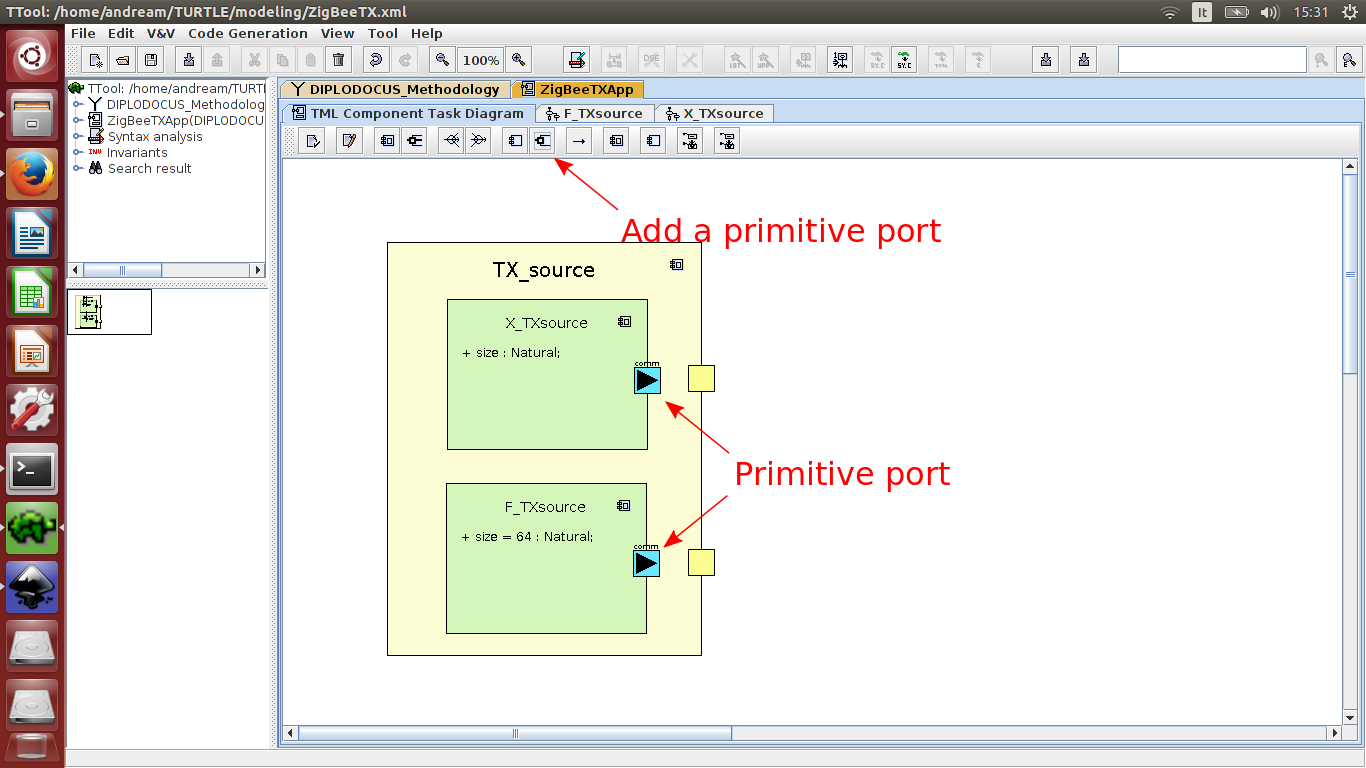
\includegraphics[width=\screenshotsize]{figures/screenshot/Ports2.png}
	\caption{The instantiation and configuration of ports for the primitive components}
	\label{fig:Ports2}
\end{figure}
%
To link a primitive port to a composite port, left-click on the \texttt{Add a connector between two ports} button. This
will automatically highlight connection points in the design (yellow squares on ports). Left-click on the connection
point of a primitive port and then left click on the connection point of a composite port. Please notice that while
primitive ports only have one connection point, composite ports have both and input (leftmost) and an output (rightmost)
connection point. Therefore, pay attention to connect the primitive ports to the input connection point of a composite port. At
this point in our design, the composite ports are not completely connected so the tool will color them in red to
highlight this syntax error. The latter can be safely ignored for the moment. The primitive ports are also
partially colored in red, Fig.~\ref{fig:Ports3}. For the \texttt{X\_} primitive component, it is correct to have a data
port, but for the \texttt{F\_} port we must change the port type to that of an event. This way, the component will be
able to exchange attribute \texttt{size} with other components. Double click on the port of component
\texttt{F\_source}, rename it as \texttt{SourceEvtOut}, select the type to be an \texttt{Event} and the first
parameter (\texttt{Type \#1}) to be of type \texttt{Natural}, Fig.~\ref{fig:Ports4_5}. Then save and close the window.
For the port attached to component \texttt{X\_source}, double click on it and rename it as \texttt{SourceChOut}. Then
select the port to be of type \texttt{Blocking}.\\
%
\begin{figure}[!htbp]
	\centering
	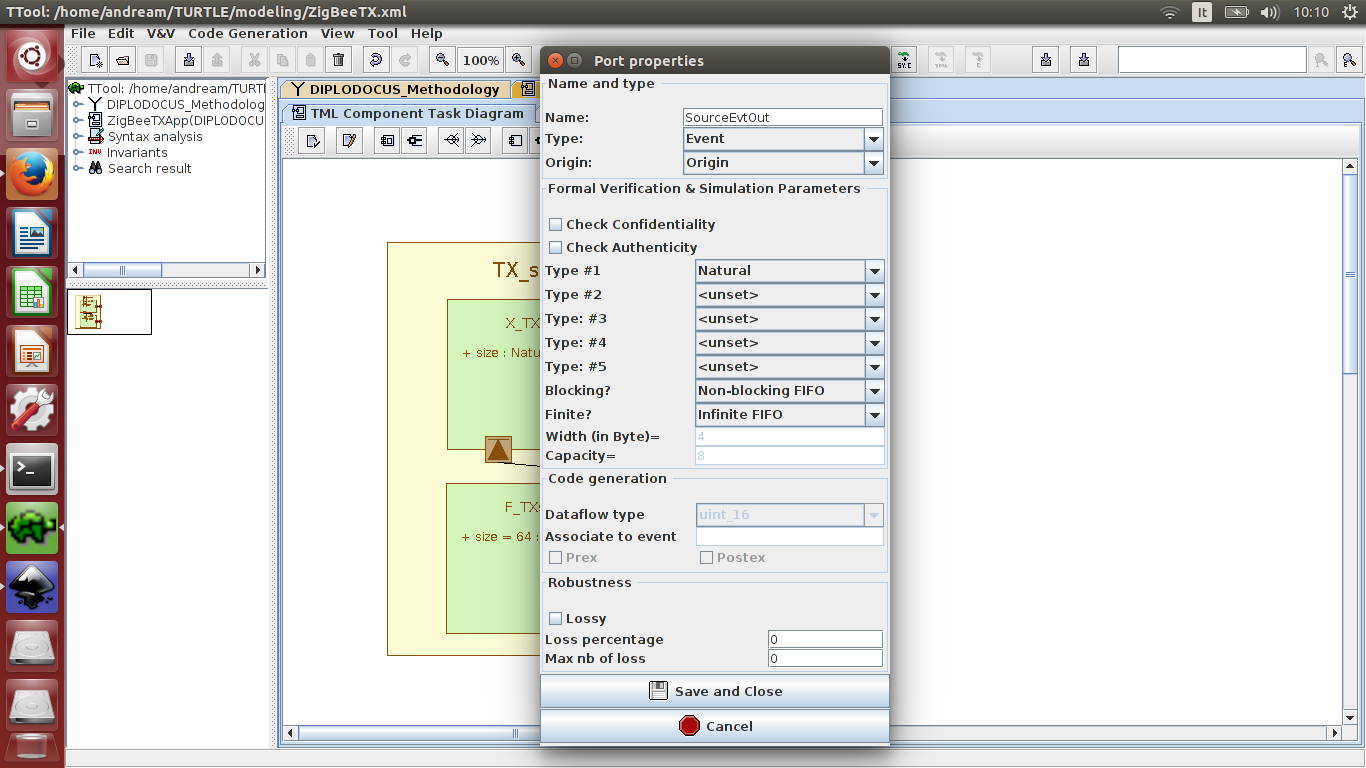
\includegraphics[width=\screenshotsize]{figures/screenshot/Ports4_5.png}
	\caption{Configuring the output event port of \texttt{F\_source}}
	\label{fig:Ports4_5}
\end{figure}
%
As mentioned above, it is the Firing primitive component that triggers the eXecution primitive component. Therefore, the
two components must be interconnected by a request that \texttt{F\_source} dispatches to \texttt{X\_source}. To
implement this in TTool/DIPLODOCUS, add another primitive port to each of the primitive components and connect them.
Then double click on the port attached to component \texttt{F\_source}, Fig.~\ref{fig:Ports4}. Rename it as
\texttt{SourceReqOut}, select the type to be a \texttt{Request} and the first parameter (\texttt{Type \#1}) of type
\texttt{Natural}, then save and close the window. Similary, rename the port attached to \texttt{X\_source} as
\texttt{SourceReqIn}, select the type to be a \texttt{Request}, select the origin to be a \texttt{Destination} port and
the first parameter (\texttt{Type \#1}) of type \texttt{Natural}, then save and close the window. Requests can carry up
to five parameters; in our case this request is used to transmit the parameter \texttt{size} of type natural.
%
\begin{figure}[!htbp]
	\centering
	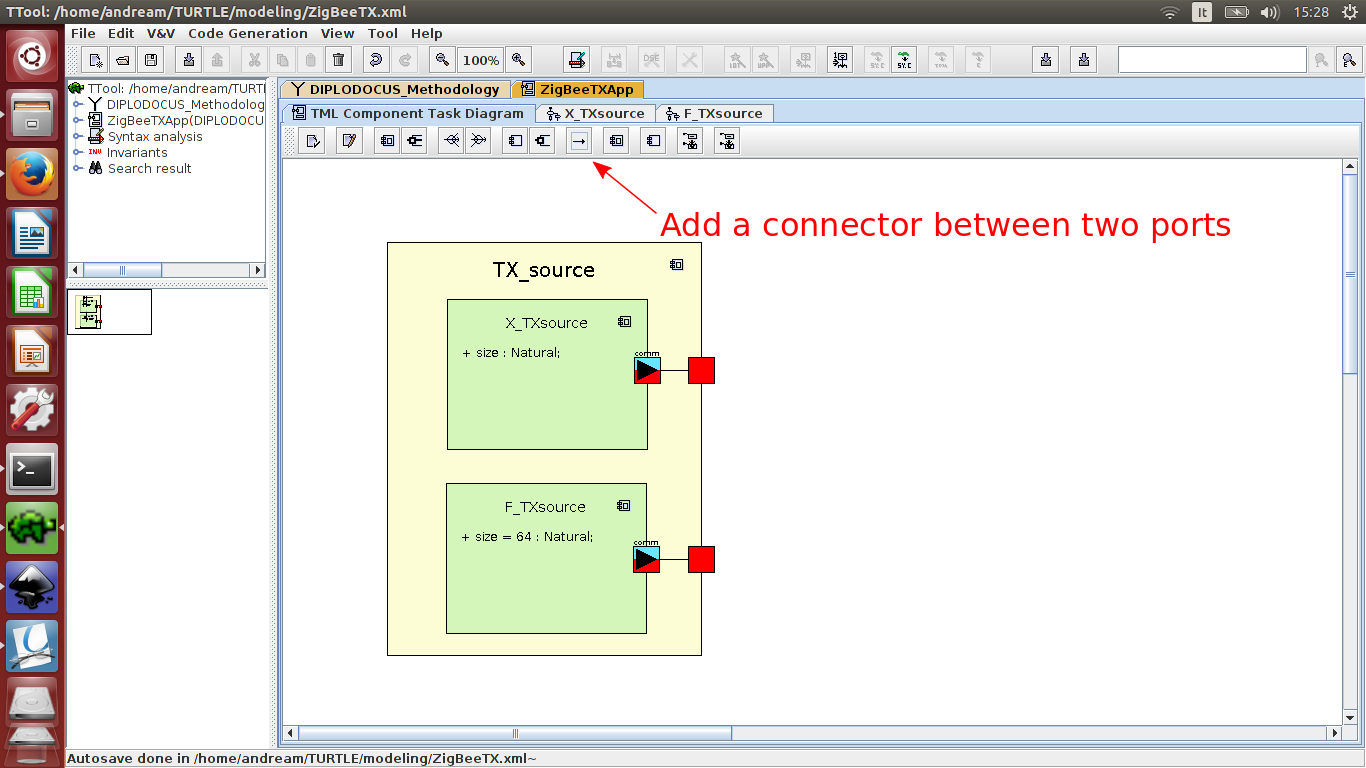
\includegraphics[width=\screenshotsize]{figures/screenshot/Ports3.png}
	\caption{Connecting primitive to composite ports}
	\label{fig:Ports3}
\end{figure}
%
\begin{figure}[!htbp]
	\centering
	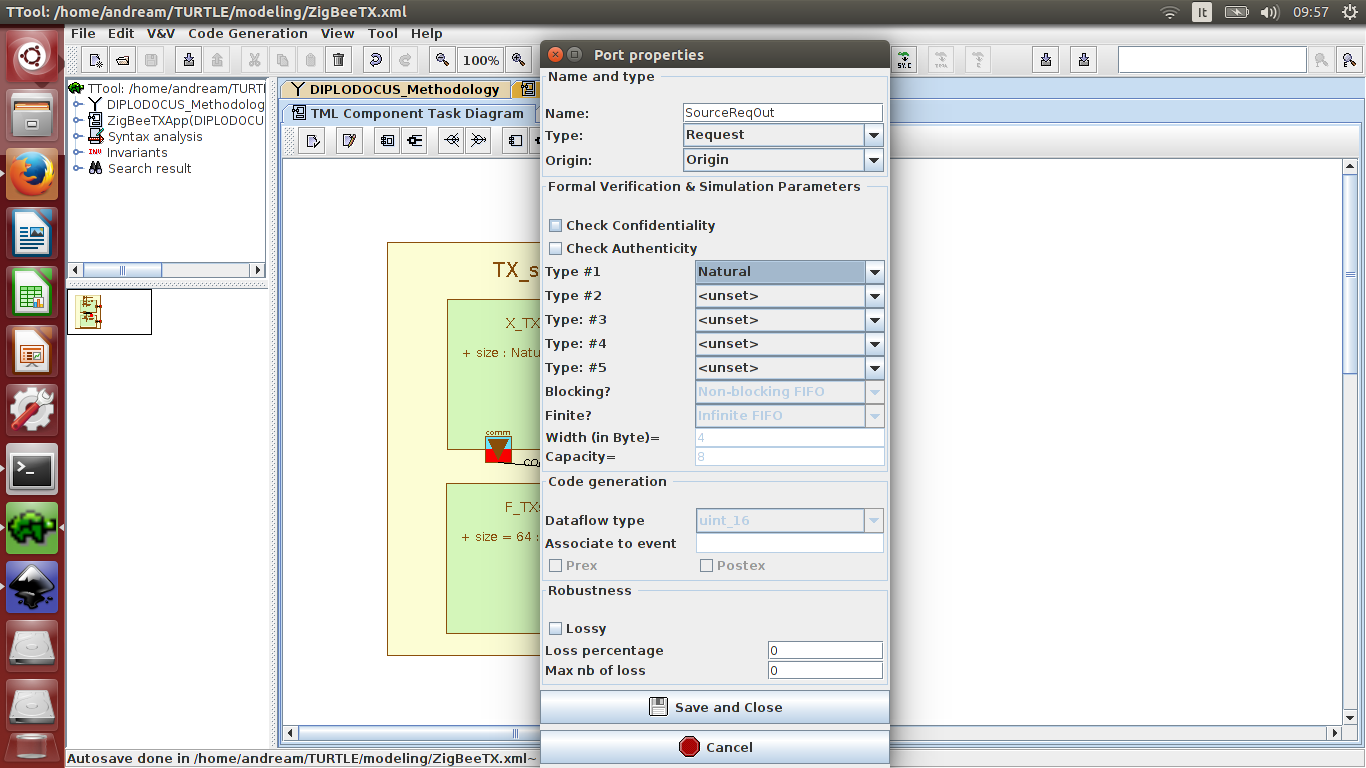
\includegraphics[width=\screenshotsize]{figures/screenshot/Ports4.png}
	\caption{Configuring the port of \texttt{F\_source} as a request}
	\label{fig:Ports4}
\end{figure}
%
The remaining buttons used to draw a \texttt{TML Component Task Diagram} (functional view of a design) are enumerated in
Fig.~\ref{fig:Buttons1} and described below:
%
\begin{enumerate}
	\item Edit TML Task Activity Diagram
	%
	\item Add a comment: add a comment to the diagram
	%
	\item Add a channel fork: allows an input channel to fork in up to 3 output channels
	%
	\item Add a channel join: allows up to 3 input channels to join into 1 channel
	%
	\item Add a reference to a composite component: allows to reference a composite component from another
	application panel
	%
	\item Add a record component
	%
	\item Show/hide internal components: shows the internal components of an application diagram, e.g., parameters
	of events and requests
	%
	\item Show/hide DIPLODOCUS IDs: show or hide the identification (natural) numbers associated to each operator
\end{enumerate}
%
\begin{figure}[!htbp]
	\centering
	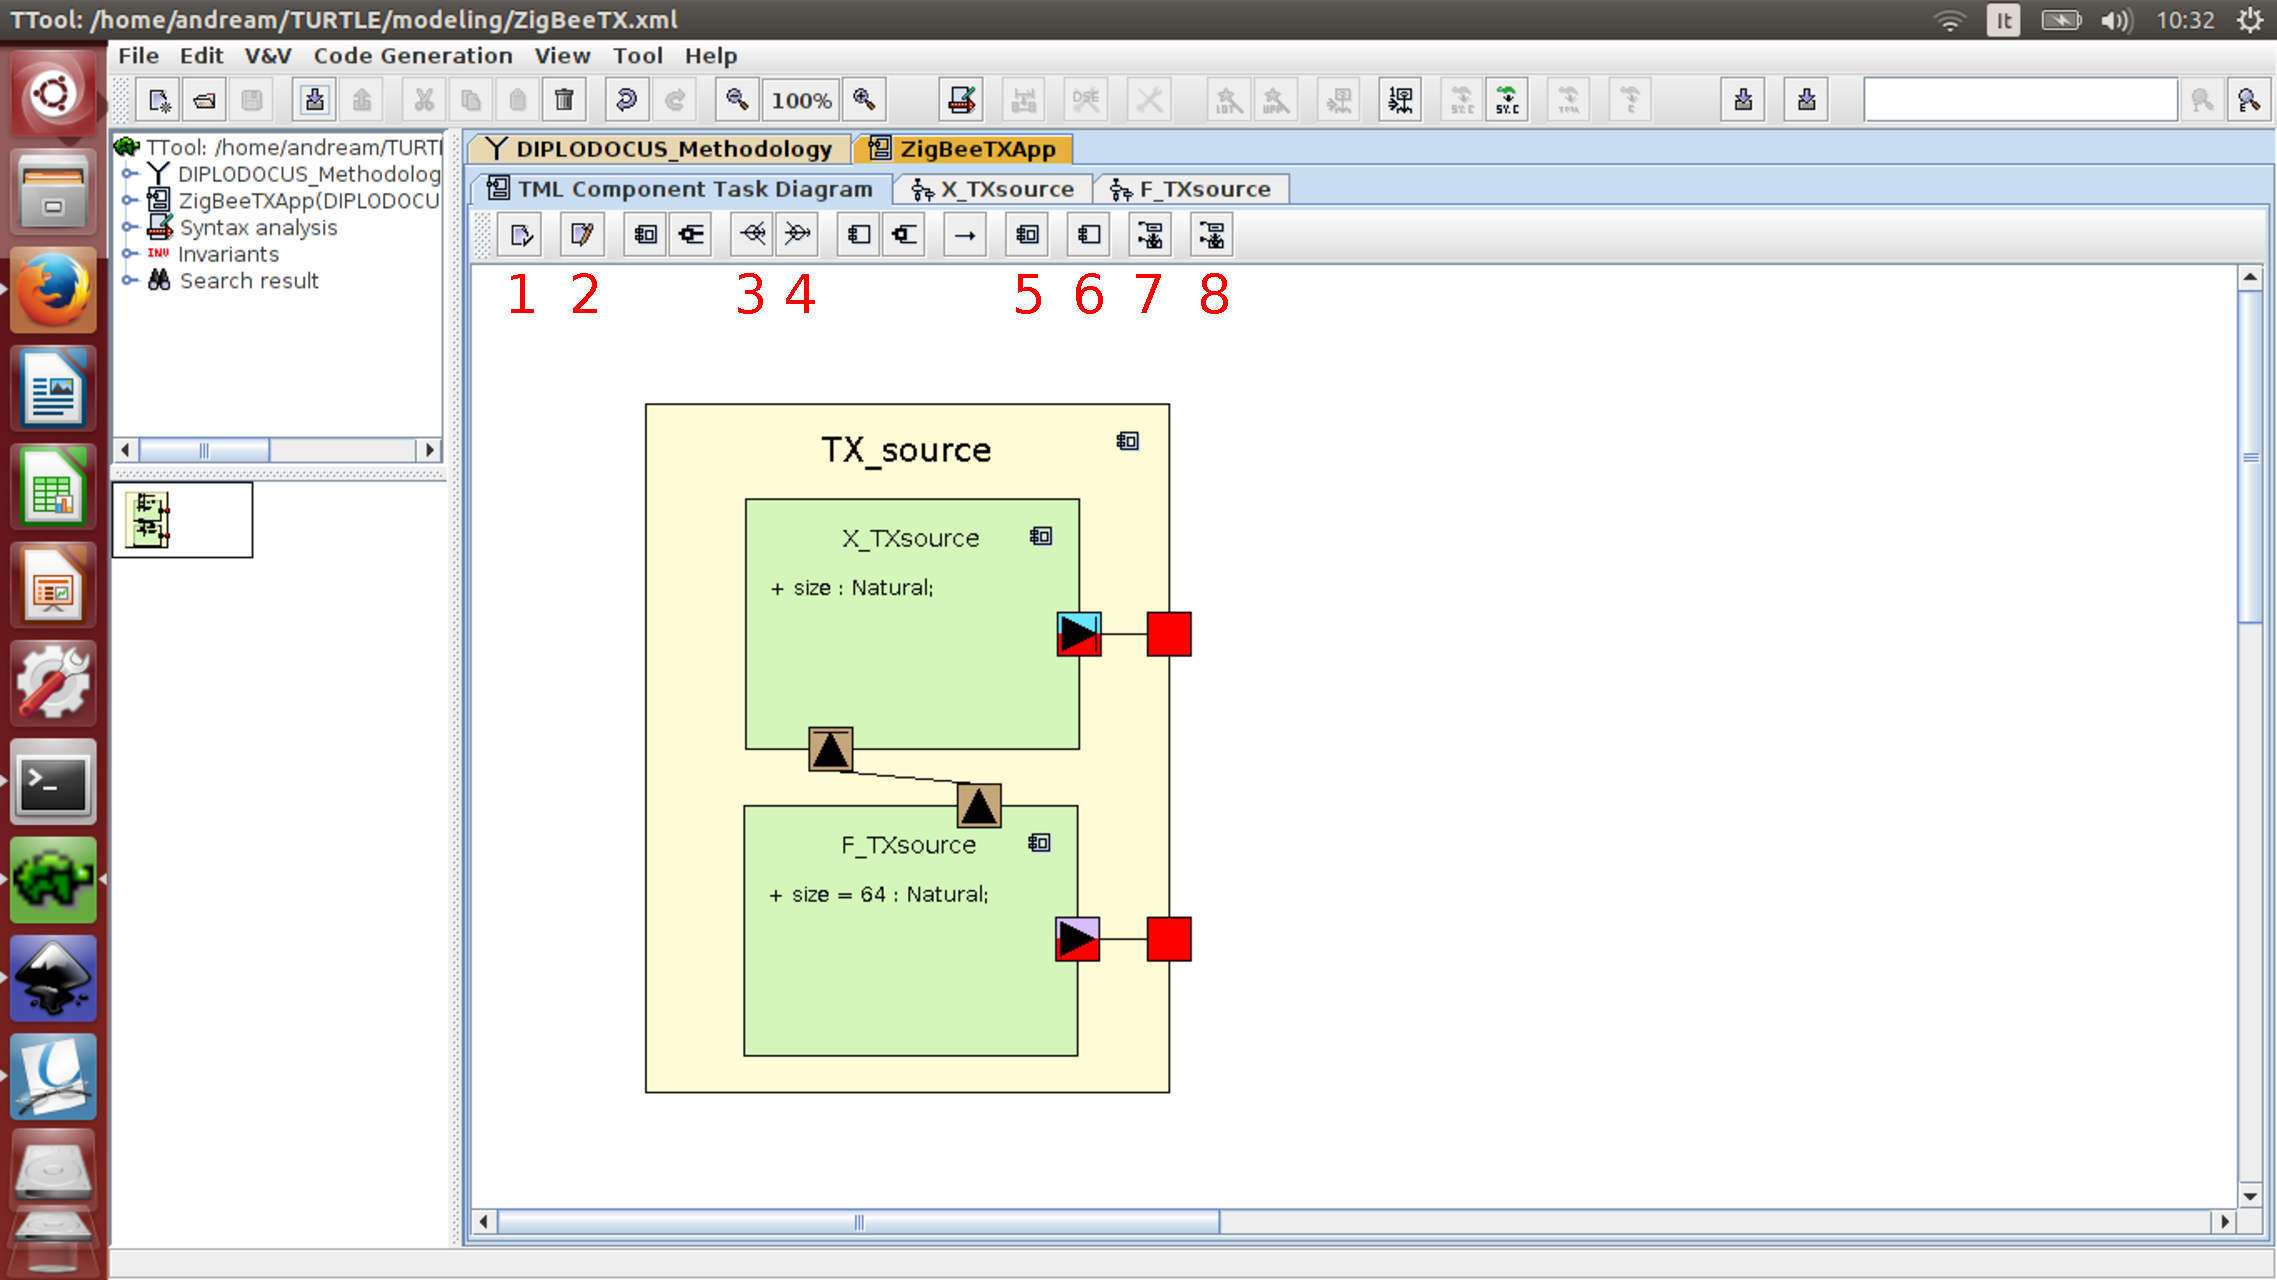
\includegraphics[width=\screenshotsize]{figures/screenshot/Buttons1.pdf}
	\caption{The buttons for the TML Composite Task Diagram enumerated}
	\label{fig:Buttons1}
\end{figure}
%
\subsubsection{The activity diagram of a primitive component}
%
As mentioned above, each primitive component has optional attributes and an activity diagram. The latter describes the
internal functionality of the component (like a state machine): the processing of data, control items and the reaction
to external events such as the reception of data or control information. In TTool/DIPLODOCUS, each primitive component
must be associated to an activity diagram.\\
%
To open the diagram window we can either click on the dedicated icon within the area of a primitive component, or open
its corresponding panel as shown in Fig.~\ref{fig:Ports5}. Let's first draw the diagram for component
\texttt{F\_source}. The design window for the diagram is dispayed in
Fig.~\ref{fig:DWindow1}. You can go back to the main diagram by right-clicking
on the design window and use ``Back to main diagram'' option.
%
\begin{figure}[!htbp]
	\centering
	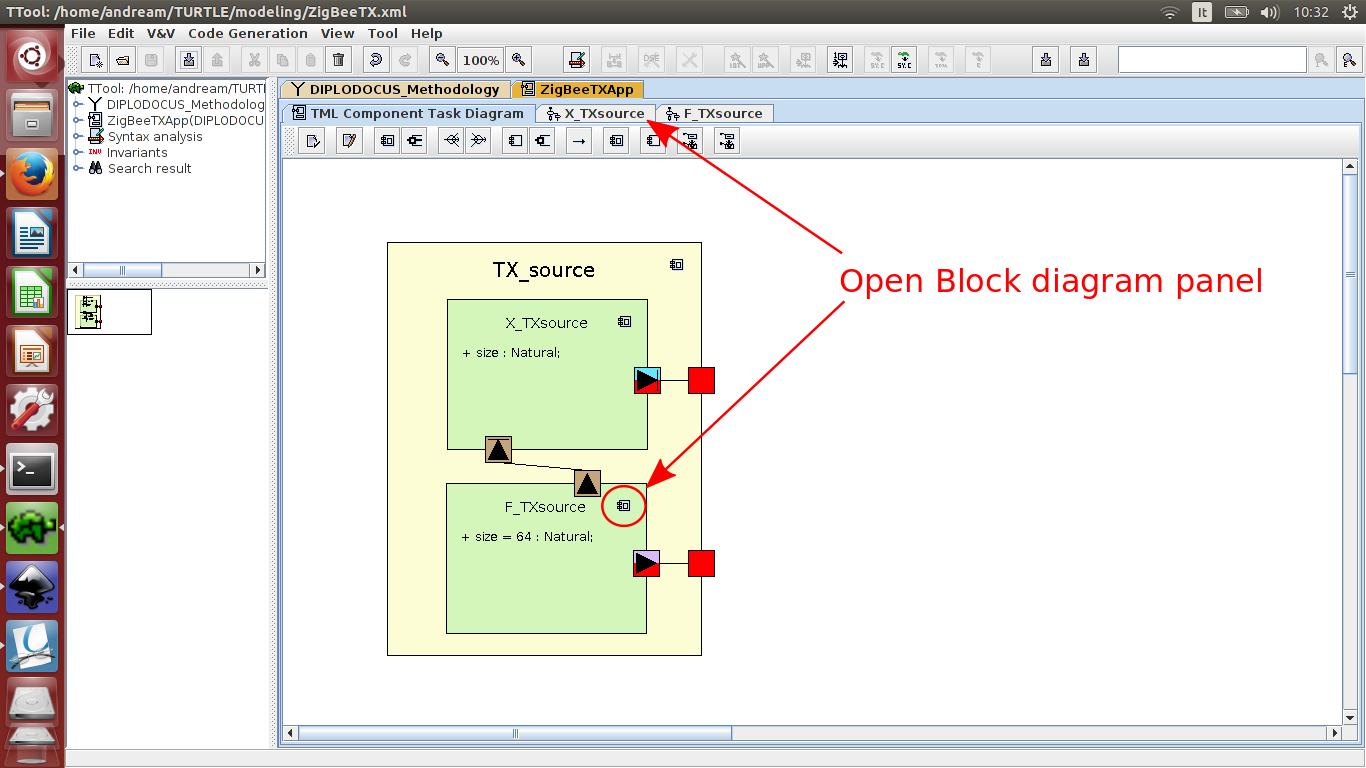
\includegraphics[width=\screenshotsize]{figures/screenshot/Ports5.png}
	\caption{Open the block diagram panel}
	\label{fig:Ports5}
\end{figure}
%
In Fig.~\ref{fig:DWindow1}, we have enumerated the buttons that are available to construct the diagram:
%
\begin{enumerate}
	\item Edit TML Task Activity Diagram
	%
	\item Add a comment: add a comment to the diagram
	%
	\item Connect two operators together: link two operators
	%
	\item Start: the starting point of a diagram's execution
	%
    \item Stop: stop the execution of the diagram or mark the end of a branch in a control structure (e.g., body of a
        for loop)
	%
	\item Write in channel: write a given amount of data to an output channel. Can be blocking or non-blocking
	according to the type of the event link (selected by user)
	%
	\item Send event: send an event and its associated attributes
	%
	\item Send request: send a request
	%
	\item Read in channel: read incoming data from a channel. Can be blocking or non-blocking according to the type
	of the event link (selected by user)
	%
	\item Wait event: wait for an incoming event. Can be blocking or non-blocking according to the type of the event
	link (selected by user)
	%
	\item Notified event: retrieve the number of incoming events received by a port. This operator tests if the event
        FIFO is not empty and returns a boolean value: if the FIFO is empty returns false, else returns the number of
        events in the FIFO.
    %
	\item Reading request arguments: retrieve arguments from a request and store the corresponding value in
	attributes
	%
	\item Action state: take an action on an attribute, e.g., increase/decrease its value
	%
	\item Choice: conditionally branch the execution of the diagram, according to boolean expressions
	%
	\item Select event: conditionally branch the execution of the diagram, according to the availability of events
        connected to the operator. This operator waits for one of the associated events to be available in the event
        FIFOs. In case several events are available in different FIFOs, then one among possible is randomly chose and
        read (consumed).% The operator returns an integer value corresponding to the event index in the provided list.
	%
	\item Loop (for): a classic for loop such as in the C language: \texttt{for(i=0;i<5;i++)}
	%
	\item Static loop (for): a loop contruct that allows the user to select the number of iterations, e.g.,
	\texttt{loop 10 times}
	%
	\item Loop for ever: loop indefinetely
	%
	\item Sequence: executes each interconnected outgoing branch in sequence.
	%
	\item Random sequence: randomly select an available operator
	%
	\item Select random: assign to an attribute a random value with uniform probability, given a range of values
	%
	\item EXECI: express the complexity of a data-processing operation as the number of computations on integer
	values
	%
	\item EXECI (time interval) express the (unknown) complexity of a integer data-processing operation as a range
	of computations on integer values
	%
	\item EXECC express the complexity of a data-processing operation as a range of computations on complex values
	%
	\item EXECC (time interval) express the (unknown) complexity of a complex data-processing operation as a range
	of computations on integer values
	%
	\item DELAY express the complexity of a data-processing operation in terms of time units
	%
	\item DELAY[,] express the (unknown) complexity of a data-processing operation in terms of a range of time
	units
	%
	\item Encryption: it can be used to indicate forging a Cryptographic Configuration and additional processing overhead due to the presence of security
	properties, see Section~\ref{sec:Security}.
	%
	\item Decryption: it can be used to recover encrypted data and indicate additional processing overhead due to the presence of security
	properties, see Section~\ref{sec:Security}.
	%
	\item Enhance
	%
	\item Show/hide internal components: has no effect on this diagram
	%
	\item Show/hide DIPLODOCUS IDs: show or hide the identification (natural) numbers associated to each operator
	%
\end{enumerate}
%
\begin{figure}[!htbp]
	\centering
	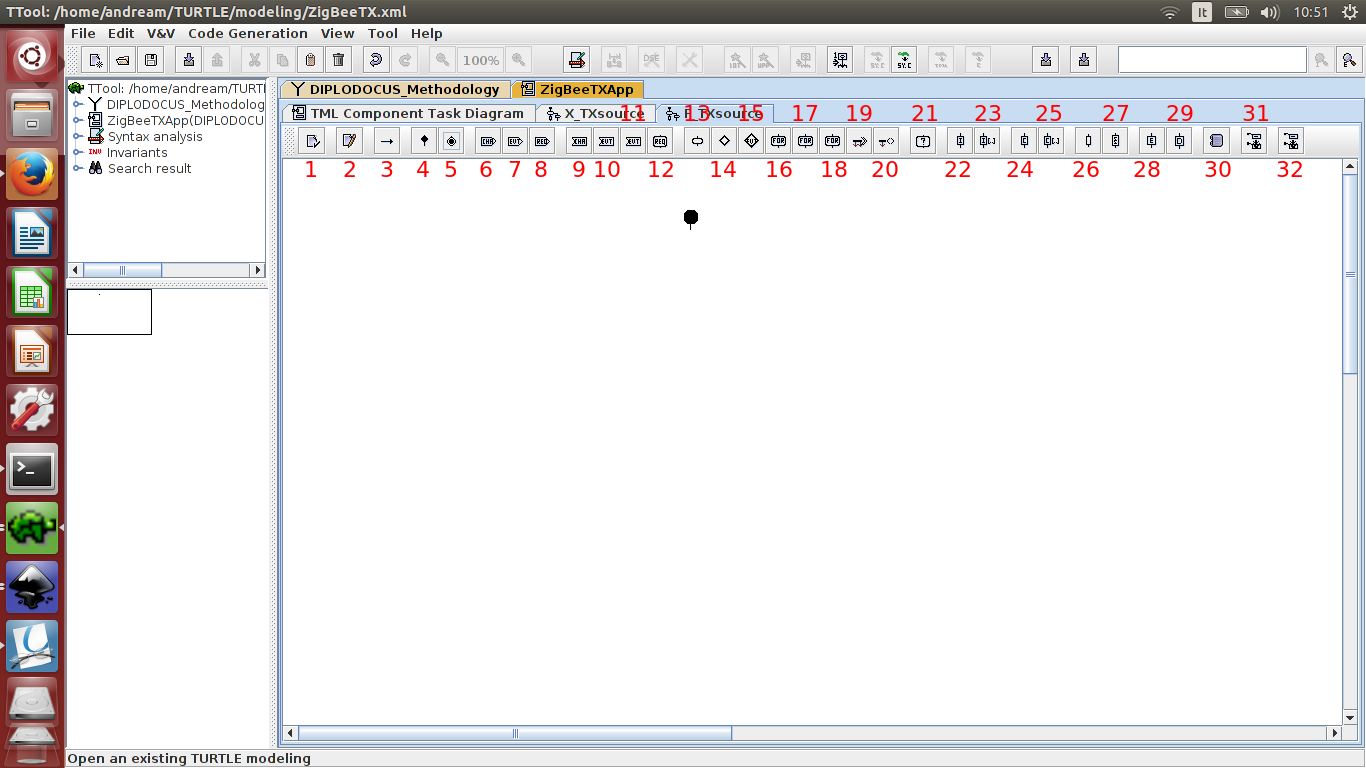
\includegraphics[width=\screenshotsize]{figures/screenshot/DWindow1.png}
	\caption{The enumerated list of the buttons available to draw the activity diagram of a primitive component}
	\label{fig:DWindow1}
\end{figure}
%
The activity diagram of component \texttt{F\_source} is depicted in Fig.~\ref{fig:ADFsource}.
%
\begin{figure}[!htbp]
	\centering
	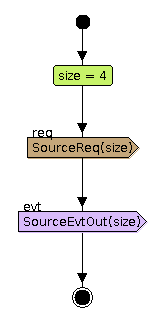
\includegraphics[width=0.15\textwidth]{figures/screenshot/ADFsource.png}
	\caption{The activity diagram of component \texttt{F\_source}}
	\label{fig:ADFsource}
\end{figure}
%
The diagram in Fig.~\ref{fig:ADFsource} is composed of the following operators interconnected in sequence: an action,
the dispatch of a request, the dispatch of an event. To instantiate these operators, simply click on the corresponding
button (Fig.~\ref{fig:DWindow1}) and then place the operator in the design area. To configure each operator, simply
double click on it, then enter the desired parameters or select the desired ports for channels, events and requests. Do
not forget to properly link the operators by means of the interconnect operator. 
%
The activity diagram of component \texttt{X\_source} is depicted in Fig.~\ref{fig:ADXsource}. It is composed of the
following operators: get the parameters of an incoming request, an EXECI operator, write data to a channel. As
described above for the operators of Fig.~\ref{fig:ADFsource}, instantiate and configure the corresponding operators.
%
\begin{figure}[!htbp]
	\centering
	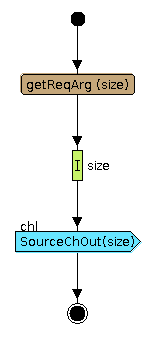
\includegraphics[width=0.15\textwidth]{figures/screenshot/ADXsource.png}
	\caption{The activity diagram of component \texttt{X\_source}}
	\label{fig:ADXsource}
\end{figure}
%
Before switching to the design of the platform model, we report in Fig.~\ref{fig:FSymbol2ChipSeq}-Fig.~\ref{fig:Xsink},
the activity diagrams of the other primitive components that constitute the
model in Fig.~\ref{fig:ZigBeeTX}. The user can draw the diagrams and interconnect the components as described so far for the single \texttt{Source} component.
%
\begin{figure}[!htbp]
	\centering
	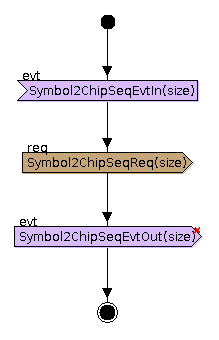
\includegraphics[width=0.20\textwidth]{figures/screenshot/F_Symbol2ChipSeq.png}
	\caption{The activity diagram of component \texttt{F\_TXSymbol2ChipSeq}}
	\label{fig:FSymbol2ChipSeq}
\end{figure}
%
\begin{figure}[!htbp]
	\centering
	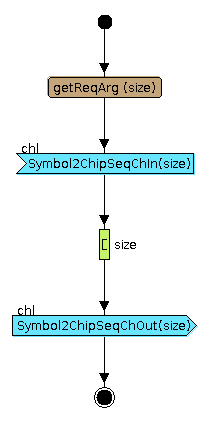
\includegraphics[width=0.20\textwidth]{figures/screenshot/X_Symbol2ChipSeq.png}
	\caption{The activity diagram of component \texttt{X\_TXSymbol2ChipSeq}}
	\label{fig:XSymbol2ChipSeq}
\end{figure}
%
\begin{figure}[!htbp]
	\centering
	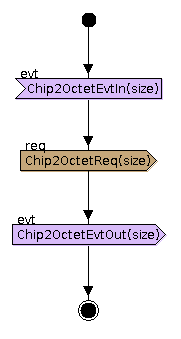
\includegraphics[width=0.15\textwidth]{figures/screenshot/F_Chip2Octet.png}
	\caption{The activity diagram of component \texttt{F\_TXChip2Octet}}
	\label{fig:FChip2Octet}
\end{figure}
%
\begin{figure}[!htbp]
	\centering
	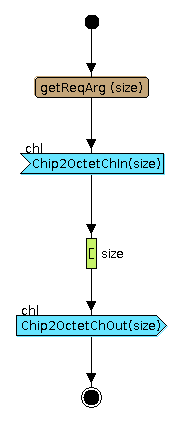
\includegraphics[width=0.15\textwidth]{figures/screenshot/X_Chip2Octet.png}
	\caption{The activity diagram of component \texttt{X\_TXChip2Octet}}
	\label{fig:XChip2Octet}
\end{figure}
%
\begin{figure}[!htbp]
	\centering
	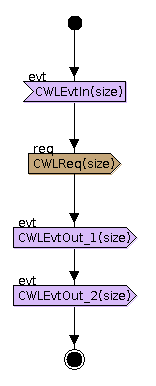
\includegraphics[width=0.15\textwidth]{figures/screenshot/F_CWL.png}
	\caption{The activity diagram of component \texttt{F\_TXCWL}}
	\label{fig:FCWL}
\end{figure}
%
\begin{figure}[!htbp]
	\centering
	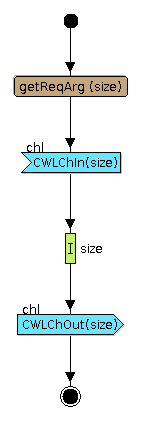
\includegraphics[width=0.15\textwidth]{figures/screenshot/X_CWL.png}
	\caption{The activity diagram of component \texttt{X\_TXCWL}}
	\label{fig:XCWL}
\end{figure}
%
\begin{figure}[!htbp]
	\centering
	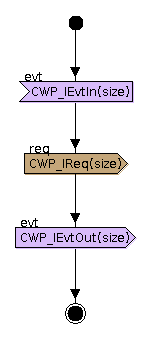
\includegraphics[width=0.15\textwidth]{figures/screenshot/F_CWP_I.png}
	\caption{The activity diagram of component \texttt{F\_TXCWPI}}
	\label{fig:FCWPI}
\end{figure}
%
\begin{figure}[!htbp]
	\centering
	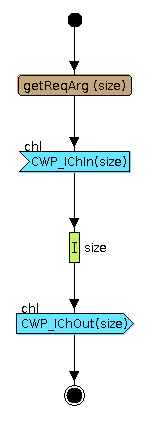
\includegraphics[width=0.15\textwidth]{figures/screenshot/X_CWP_I.png}
	\caption{The activity diagram of component \texttt{X\_TXCWPI}}
	\label{fig:XCWPI}
\end{figure}
%
\begin{figure}[!htbp]
	\centering
	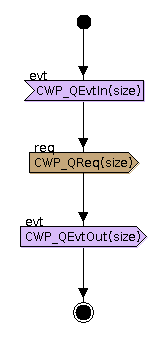
\includegraphics[width=0.15\textwidth]{figures/screenshot/F_CWP_Q.png}
	\caption{The activity diagram of component \texttt{F\_TXCWPQ}}
	\label{fig:FCWPQ}
\end{figure}
%
\begin{figure}[!htbp]
	\centering
	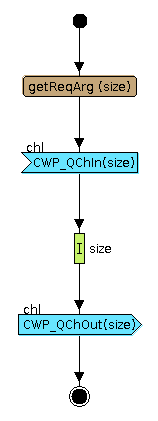
\includegraphics[width=0.15\textwidth]{figures/screenshot/X_CWP_Q.png}
	\caption{The activity diagram of component \texttt{X\_TXCWPQ}}
	\label{fig:XCWPQ}
\end{figure}
%
\begin{figure}[!htbp]
	\centering
	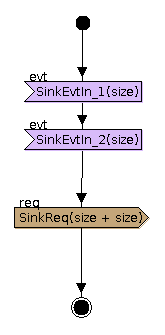
\includegraphics[width=0.15\textwidth]{figures/screenshot/F_Sink.png}
	\caption{The activity diagram of component \texttt{F\_TXsink}}
	\label{fig:Fsink}
\end{figure}
%
\begin{figure}[!htbp]
	\centering
	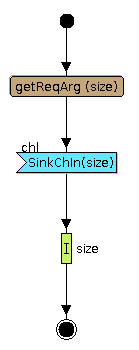
\includegraphics[width=0.15\textwidth]{figures/screenshot/X_Sink.png}
	\caption{The activity diagram of component \texttt{X\_TXsink}}
	\label{fig:Xsink}
\end{figure}
%
%
%
\newpage
\subsection{Platform modeling}
\label{subsec:Embb}
%
In this sub-section, we continue our design of the ZigBee transmitter (data-link layer) and discuss the model of the
target hardware/software platform, Fig.~\ref{fig:PsiChartArch}.\\
%
\begin{figure}[htbp]
	\centering
	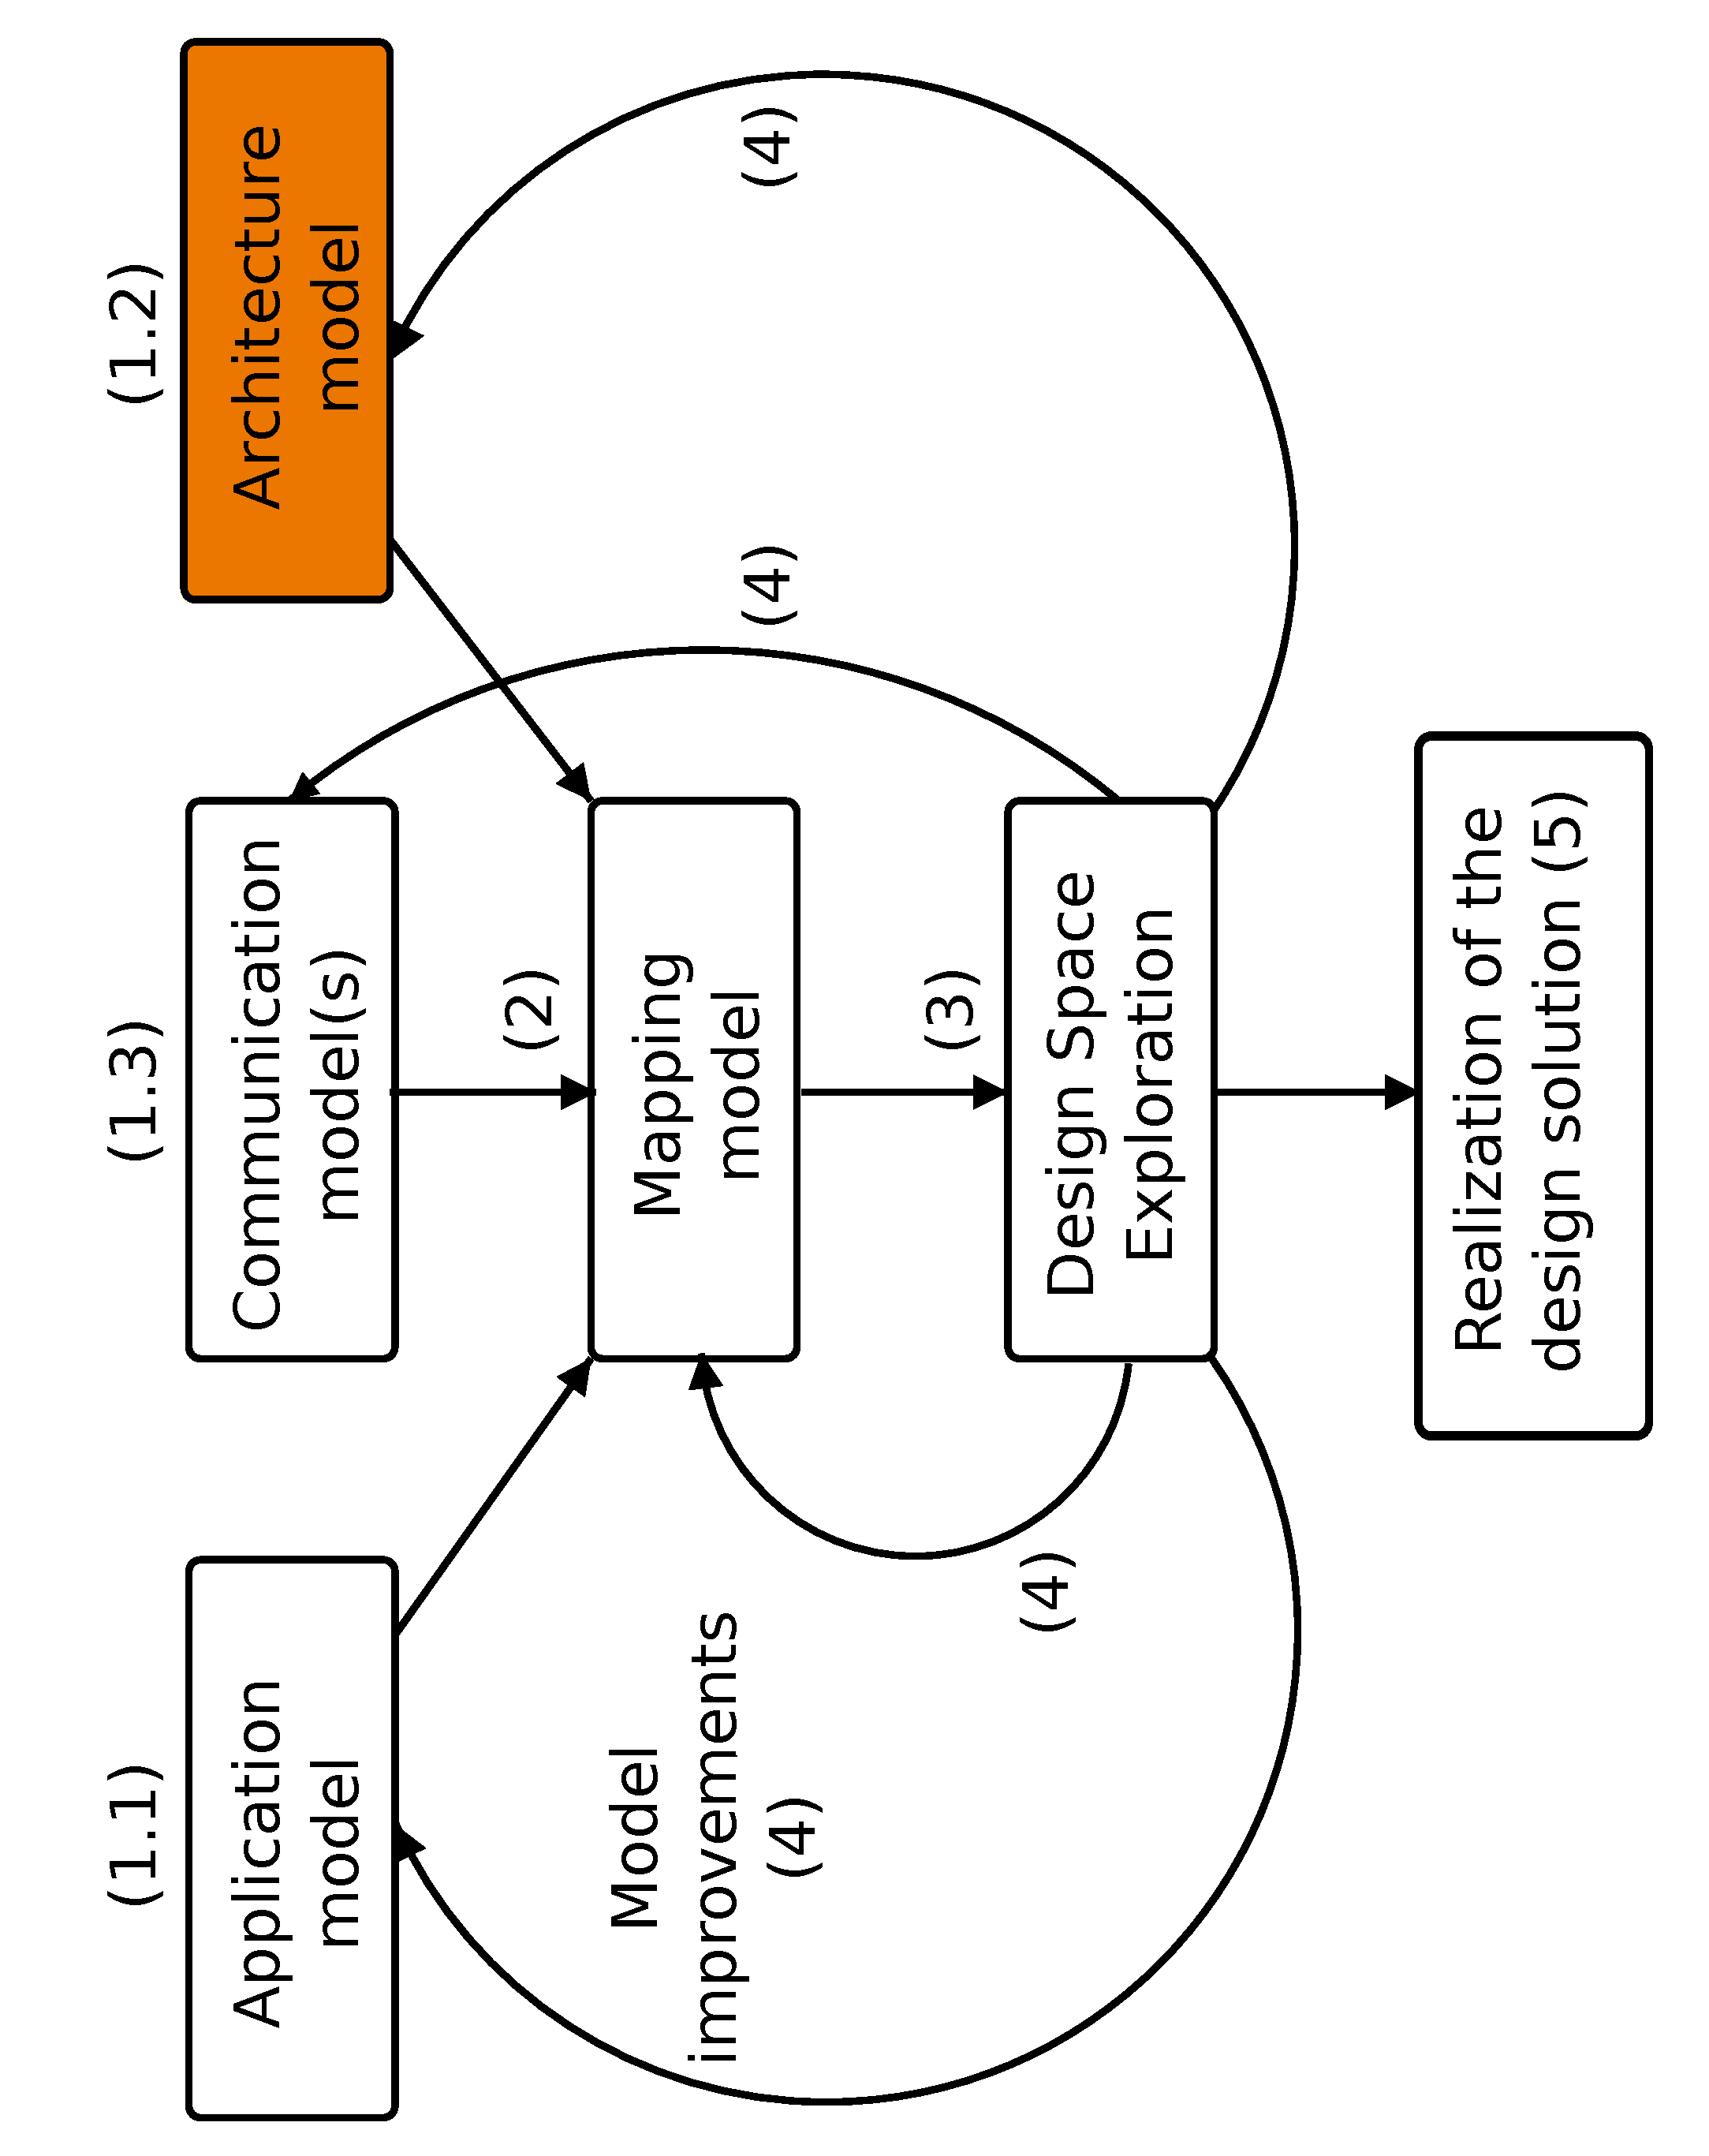
\includegraphics[angle=-90,origin=c,width=0.4\textwidth]{figures/PsiChartArch.pdf}
	\caption{The step of modeling the hardware/software platform, that is described in this section, in the context of
        the $\Psi$-chart design approach}
	\label{fig:PsiChartArch}
\end{figure}
The target platform for our case study is EMBB~\cite{Embb}, a generic baseband architecture dedicated to signal
processing applications.\\
%
Fig.~\ref{fig:EmbbArch}a shows the UML Deployment Diagram of the EMBB architecture. EMBB is composed of a Digital Signal
Processing part (DSP part) and a general purpose control processor (the main CPU). In the DSP part, left-hand side of
Fig.~\ref{fig:EmbbArch}a, samples coming from the air are processed in parallel by a distributed set of Digital Signal
Processing Units (DSPU1 through DSPUn) interconnected by a crossbar (Crossbar). Fig.~\ref{fig:EmbbArch}b illustrates the
internal architecture of a DSPU: each unit is equipped with a local micro-controller ($\mu$C) that allows to reduce the
intervention of the main CPU, a Processing Sub-System (PSS), a computational unit, and a Direct Memory Access controller
(DMA) to transfer data in and out of the DSPU's local memory (the Memory Sub-System, MSS). The latter is mapped on the
global address map of the main CPU and is accessible by the DMAs, the $\mu$Cs and the system interconnect. The system
interconnect permits exchanges of control and data items: it is composed of a crossbar (Crossbar), a bridge (Main
Bridge) and a main bus (Main Bus).
%
The system interconnect is shared between the DSP part and the main CPU, where the control operations of an application
are executed. The main CPU is in charge of configuring and controlling the processing operations performed by the DSPUs
and the data transfers. The main CPU has direct access to a memory unit (MAINmemory) and a bus interconnect (MAINbus)
that communicates with the DSP part via the Main Bridge.
%
\begin{figure}[!htbp]
	\centering
	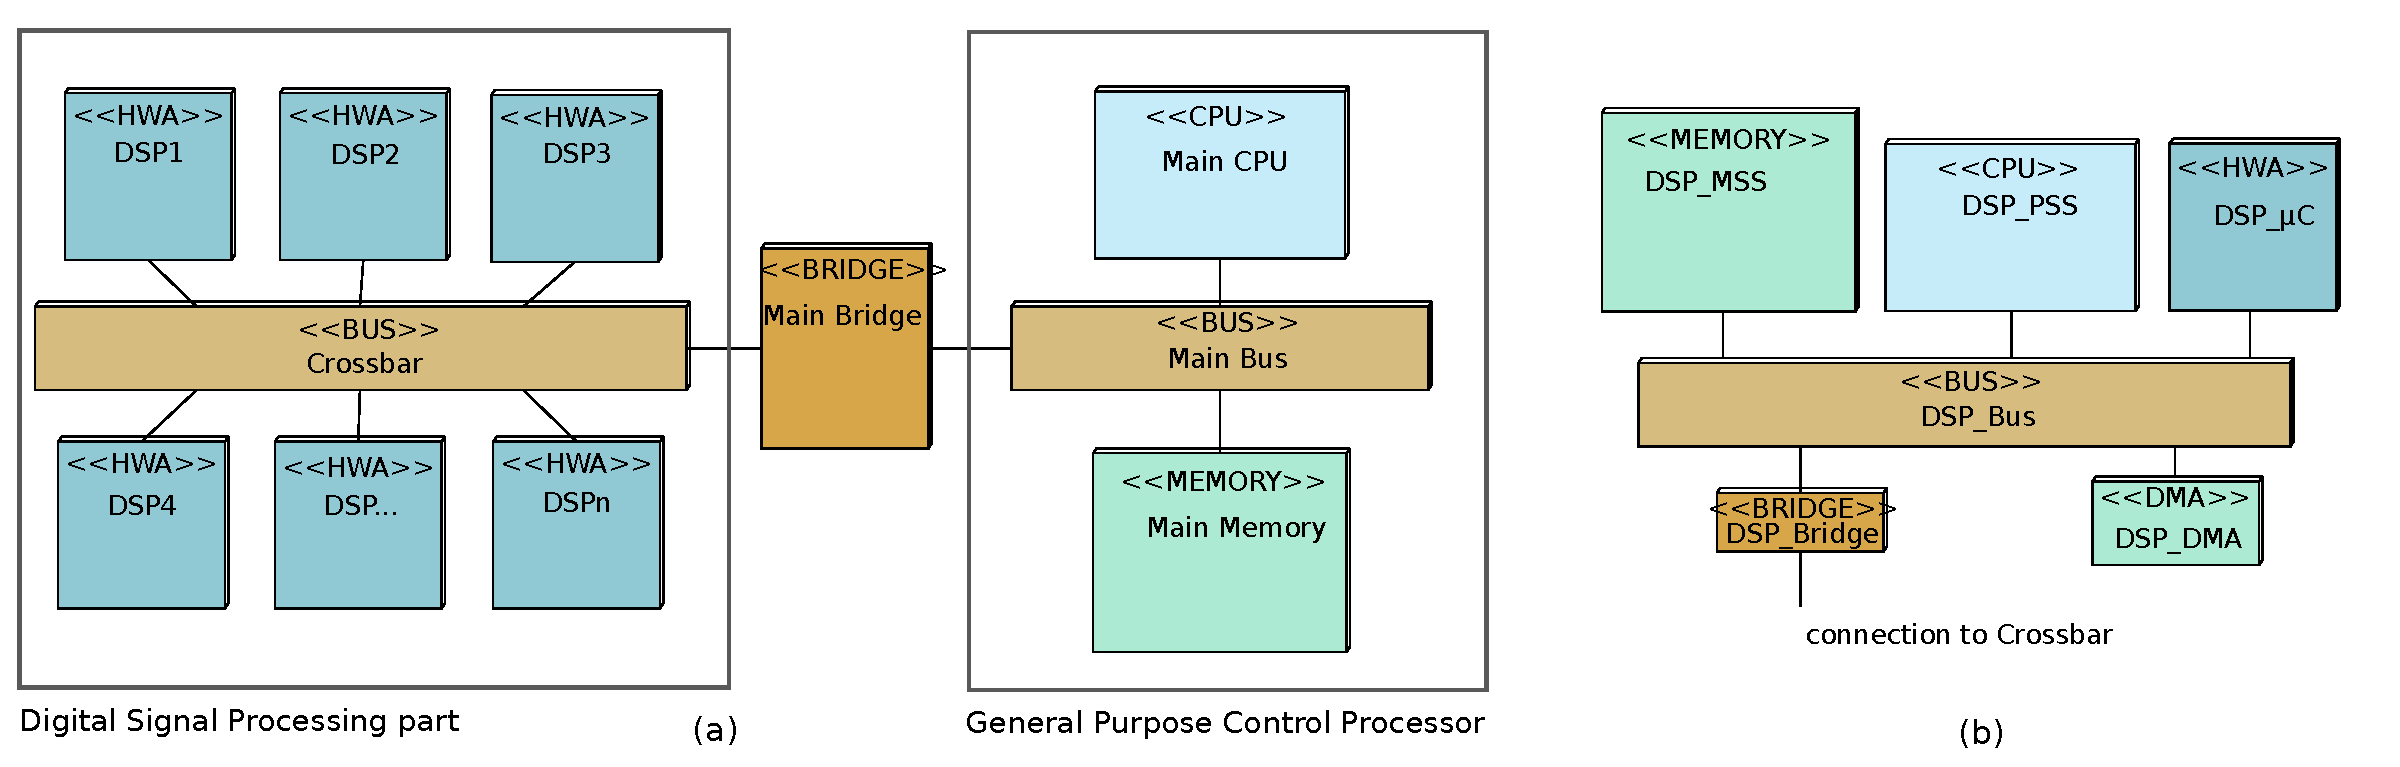
\includegraphics[width=\textwidth]{figures/Embb_BlockDiagram.pdf}
    \caption{The UML Deployment Diagrams (architecture view) of an instance of EMBB, part (a), with its Digital Signal
    Processing part (left side) and main CPU (right side). Part (b) shows the internal architecture of each DSP unit.}
 	\label{fig:EmbbArch}
\end{figure}
%
\\According to our design experience with the EMBB platform, the best configuration for signal-processing applications in
terms of performance is the one with the following four DSP units:
%
\begin{itemize}
	\item Front End Processor (FEP): it implements Discrete Fourier Transform and vector processing operations.
	%
	\item Interleaver (INTL): it implements permutations (i.e., interleaving and de-interleaving) of sequences of data
	samples.
	%
	\item Mapper (MAPPER): it transforms a frame of input symbols into a frame of complex numbers representing the
	points of a 2D constellation diagram, via Look-Up-Tables.
	%
	\item Analog to Digital-Digital to Analog Interface (ADAIF): a dispatcher that is capable of receiving up to 4 input
	streams from 4 A/D converters and of transmitting up to 4 output streams to 4 D/A converters.
\end{itemize}
%
Therefore, the platform model that we will describe next is composed of the above DSP units.
%
\subsection{Creating the platform model of EMBB}
\label{subsec:Create-Embb}
%
To create a platform model in TTool/DIPLODOCUS, right-click in the panel tab and select \texttt{New Partitioning -
Architecture and Mapping}. This will open the panel in Fig.~\ref{fig:Platform} where the buttons available to design a
new model have been enumerated. As we did for the application panel, we rename the platform panel as \texttt{EMBB}
(right click, then \texttt{Rename}).
%
\begin{figure}[!htbp]
	\centering
	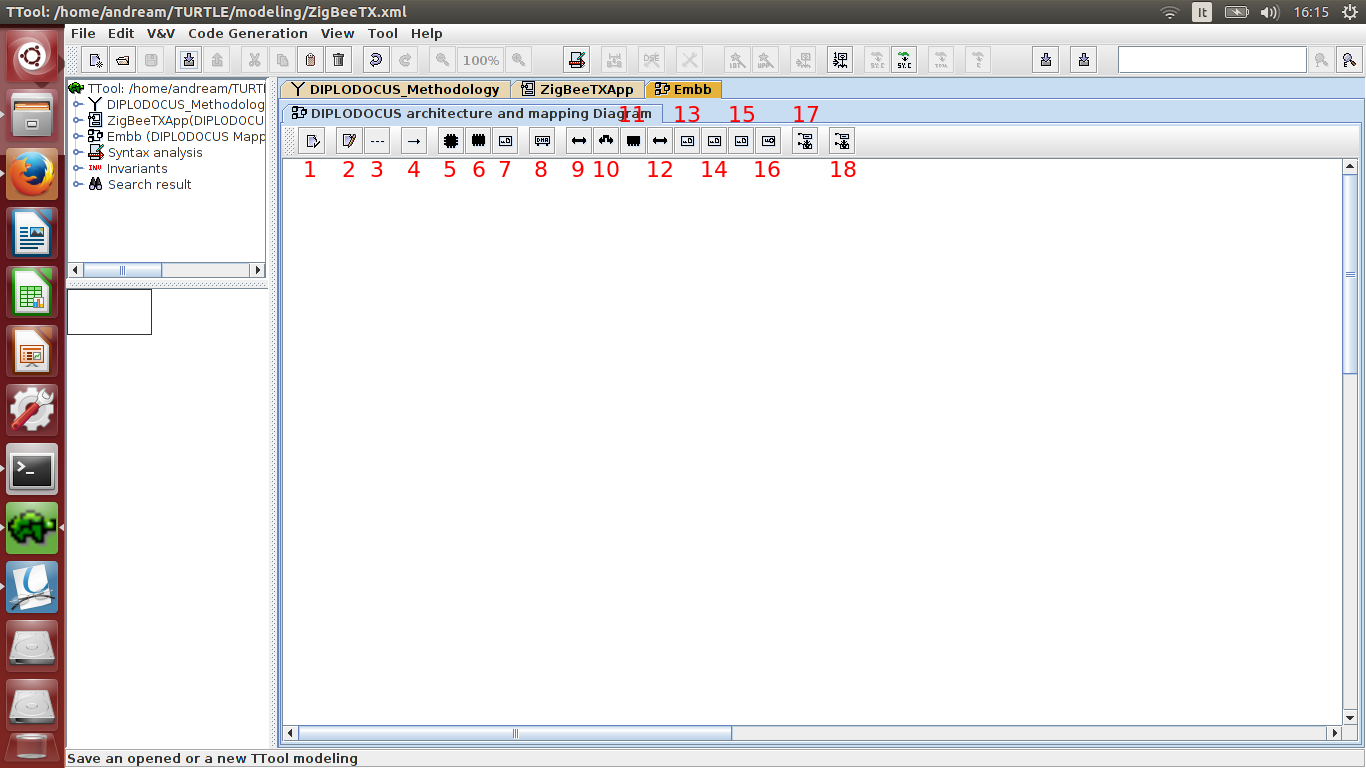
\includegraphics[width=\screenshotsize]{figures/screenshot/Platform.png}
	\caption{The design area for the platform model and the enumerated list of available buttons.}
 	\label{fig:Platform}
\end{figure}
%
These buttons are described below:
%
\begin{enumerate}
	\item Edit DIPLODOCUS Architecture Diagram
	%
	\item Add a comment: add a comment to the diagram
	%
	\item Comment connector
	%
	\item Connect two operators together: link two operators
	%
	\item CPU node: instantiate a node for a generic CPU block
	%
	\item Hardware accelerator node: instantiate a node for a generic hardware accelerator block
	%
	\item Map a task: map a primitive component from an application diagram onto a platform unit
	%
	\item DMA node: instantiate a node for a generic DMA block
	%
	\item Bus node: instantiate a node for a generic bus block
	%
	\item Bridge node: instantiate a node for a generic bridge block
	%
	\item Memory node: instantiate a node for a generic memory block
	%
	\item CP node: instantiate a node to map a Communication Pattern
	%
	\item Map an event/request: map an event/request onto platform unit
	%
	\item Map a channel: map a channel onto a memory unit, a bus or a bridge unit
	%
	\item Map a port: map a port onto the Communication Pattern mapping node
	%
	\item Map a key: it can be used to map an encryption/decryption key when the design also accounts for security
        properties, see Section~\ref{sec:Security}.
	%
	\item Show/hide internal components: has no effect on this diagram
	%
	\item Show/hide DIPLODOCUS IDs: show or hide the identification (natural) numbers associated to each operator
	%
\end{enumerate}
%
To draw the platform diagram of Fig.~\ref{fig:EmbbArch}, the user must simply instantiate the desired units by clicking on
the corresponding buttons, placing the units in the design area, interconnecting them, and assigning to each unit the
correct performance parameters. With respect to Fig.~\ref{fig:EmbbArch}b, each DSP unit is composed of a CPU block
modeling the PSS, a memory block modeling the PSS's local memory. In this case study, we do not consider the
micro-controllers of each DSP unit. Moreover, as the DMA units are not supported by the simulator, we model them as CPU
blocks instead. Thus, a DSP unit results to be composed of 2 CPU blocks and a memory block interconnected by a local
bus. The latter is then linked to the crossbar interconnect via a bridge. The crossbar interconnect itself is modeled as
a bus. The control part of EMBB, left hand-side of Fig.~\ref{fig:EmbbArch}a, is simply modeled as a generic CPU unit
interconnected to a memory unit via a bus. This bus is itself connected to the crossbar interconnect via a bridge
unit. Fig.~\ref{fig:SamplePlatform} shows an excerpt of the platform model with the control part of EMBB on the right
hand-side and two DSP units (Mapper and Interleaver) on the left hand-side.\\
%
In this design we do not use the local microcontrollers of each DSP unit, therefore our platform model does not include
them. However, their modeling is very simple as it simply requires us to instantiate a CPU unit and to connect it to the
internal bus of each DSP unit.
%
\begin{figure}[!htbp]
	\centering
	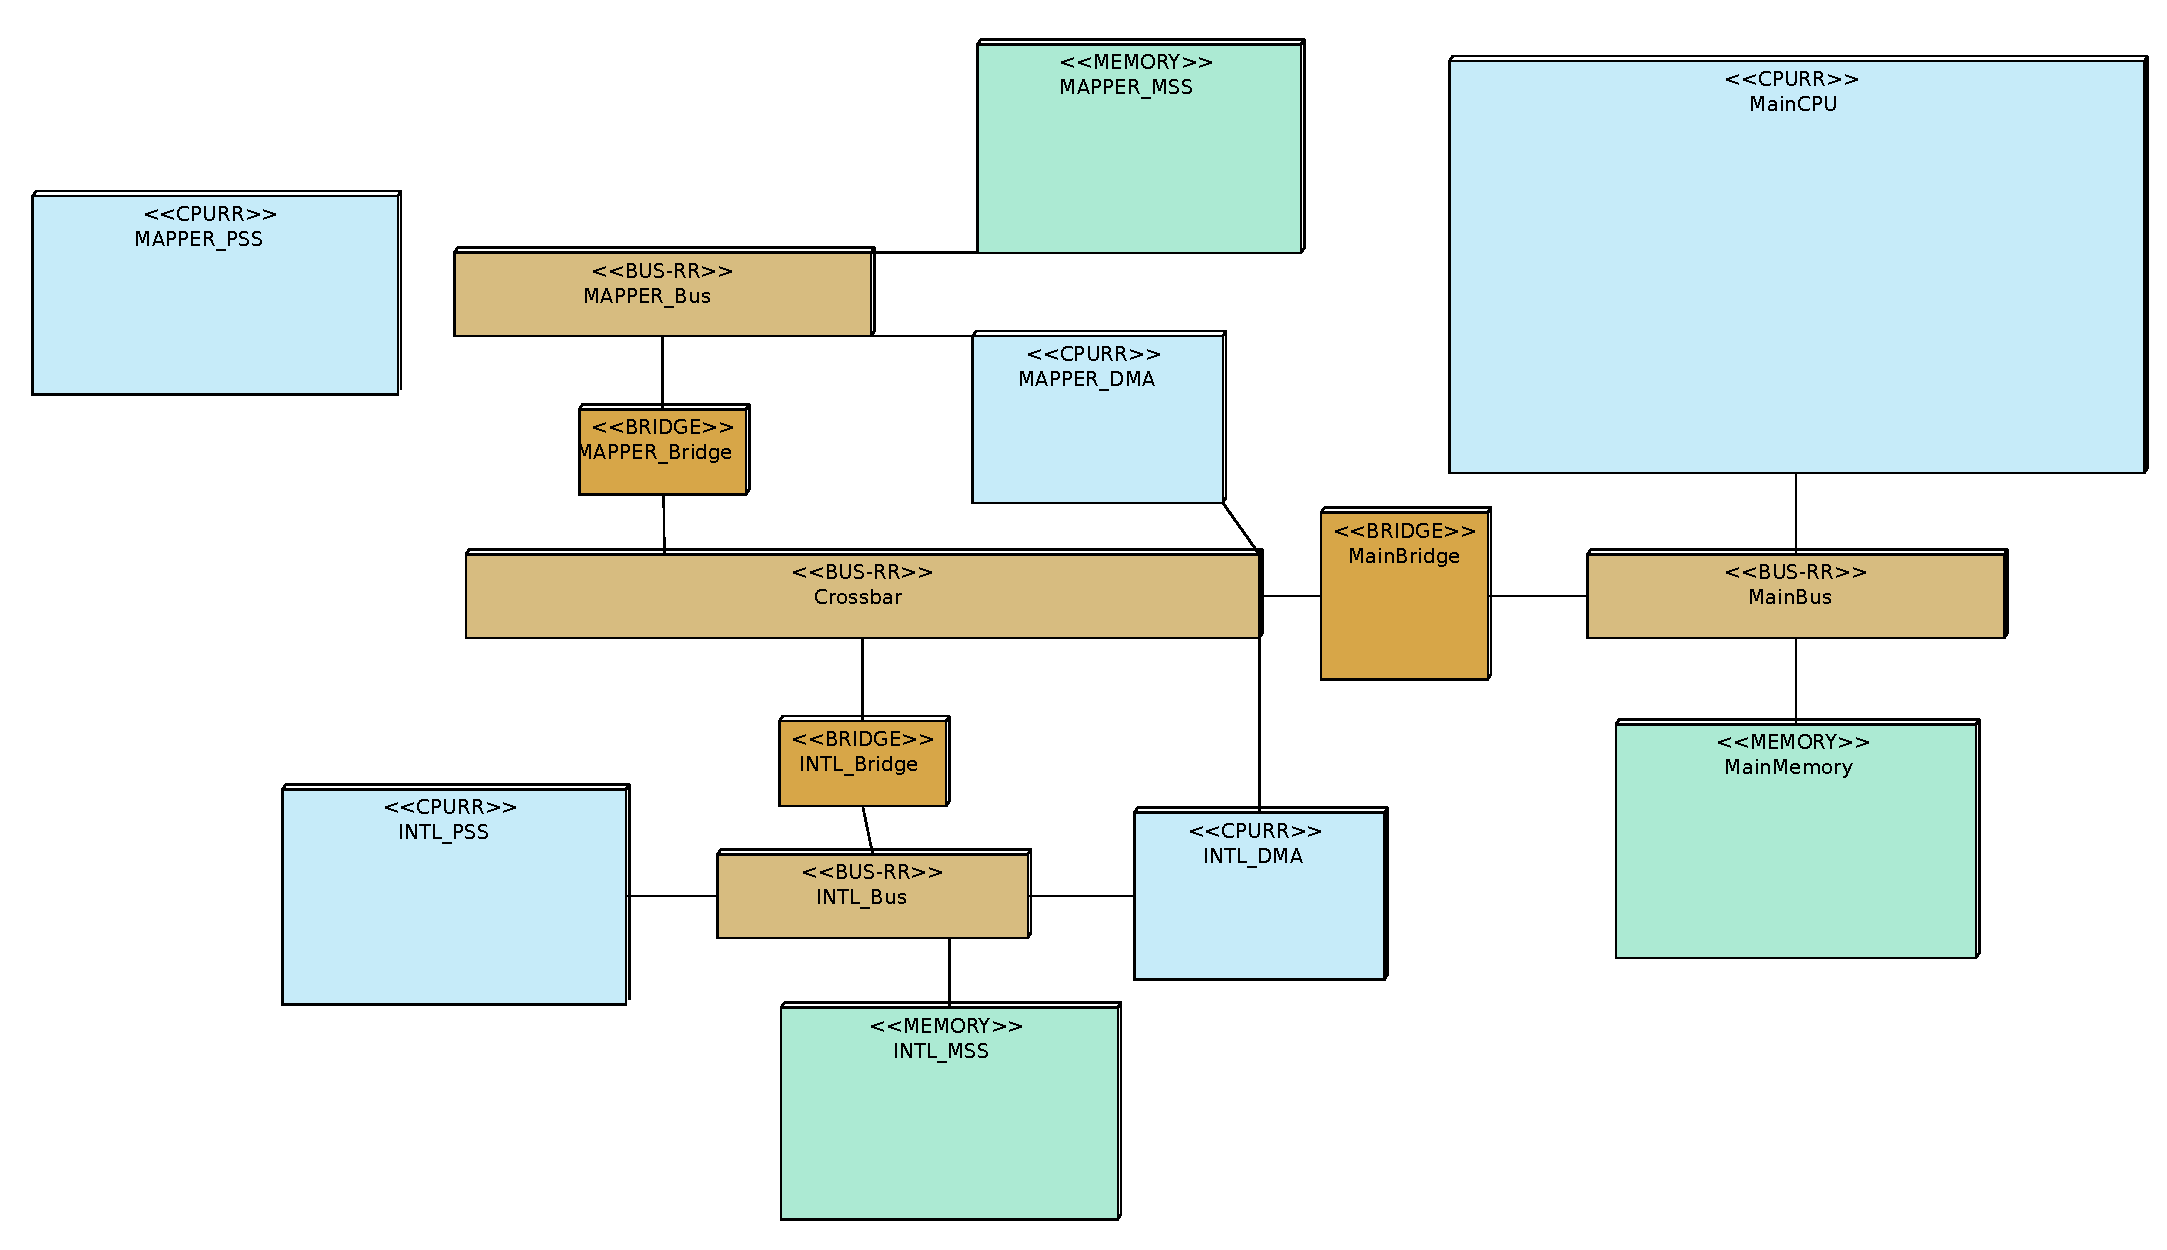
\includegraphics[angle=-90,origin=c,height=0.9\paperwidth]{figures/evaluation/Excerpt.pdf}
    \caption{An excerpt of the platform model of EMBB}
	\label{fig:SamplePlatform}
\end{figure}
%
%
\\In the following tables we summarize the list of parameters that are associated to each generic platform unit and we
provide a description of their meaning from the perspective of the simulation engine (Section~\ref{sec:DSE}). We specify
here that parameters such as the pipeline size and the branching miss rate of a CPU impact the simulation time. For more
details, please refer to Appendix\ref{app:SimuSemantics}.
%
\begin{table}[!htbp]
\begin{center}
	\caption{The performance parameters of a generic CPU unit}
	\label{tab:PerfParamCPU}
	\begin{tabular}{| >{\centering\arraybackslash}p{7cm} | >{\centering\arraybackslash}p{7cm} |} \hline
	\textbf{Parameter}				& \textbf{Semantics}	\\ \hline
	Arbitration policy				& The arbitration policy used by the OS to schedule mapped
	tasks\\ \hline
	Slice time (microseconds)			& The maximum time allocated by the OS scheduler to execute a task\\
	\hline
	Number of cores					& The number of cores of the CPU\\ \hline
	Data size (bytes)				& The size of an EXECI/EXECC operation, in number of bytes\\
	\hline
        Pipeline size (num. stages)			& The number of stages of the pipeline\\ \hline
	Task switching time (cycles)			& The time taken by the OS for a context switch\\ \hline
	Miss branching prediction (in \%)		& The miss percentage of the CPU branch prediction scheme\\
	\hline
	Cache miss (in \%)				& The percentage of cache misses\\ \hline
	Go idle time (cycles)				& The time taken by the OS and the CPU hardware to go idle\\ \hline
	Max consecutive cycles before idle (cycles)	& Number of consecutive cycles of NOPs before the CPU goes idle\\ \hline
	EXECI (cycles)					& The number of clock cycles corresponding to an integer
	operation \\ \hline
	EXECC (cycles)					& The number of clock cycles corresponding to an operation on
	complex numbers \\ \hline
	Clock divider					& This number defines the operating clock frequency of the
	CPU.
	It is expressed via a number that is used to divide the global design frequency, whose default value is 200 MHz.
	Thus a clock divider equal to 4 means that the CPU operates at 200/4 = 50 MHz
	\\
	\hline
	\end{tabular}
\end{center}
\end{table}
%
\begin{table}[!htbp]
\begin{center}
	\caption{The performance parameters of a generic hardware accelerator unit}
	\label{tab:PerfParamHwA}
	\begin{tabular}{| >{\centering\arraybackslash}p{7cm} | >{\centering\arraybackslash}p{7cm} |} \hline
	\textbf{Parameter}				& \textbf{Semantics}	\\ \hline
	Data size (bytes)				& The size of an EXECI/EXECC operation, in number of bytes\\
	\hline
	EXECI execution time (cycles)			& The number of clock cycles expressed as an integer\\
	\hline
	Clock divider					& This number defines the operating clock frequency of the CPU.
	It is expressed via a number that is used to divide the global design frequency, whose default value is 200 MHz.
	Thus a clock divider equal to 4 means that the CPU operates at 200/4 = 50 MHz\\
	\hline
	\end{tabular}
\end{center}
\end{table}
%
\begin{table}[!htbp]
\begin{center}
	\caption{The performance parameters of a generic DMA unit}
	\label{tab:PerfParamDMA}
	\begin{tabular}{| >{\centering\arraybackslash}p{7cm} | >{\centering\arraybackslash}p{7cm} |} \hline
	\textbf{Parameter}				& \textbf{Semantics}	\\ \hline
	Data size (bytes)				& Number of bytes that can be transferred in a clock cycle \\ \hline
	Number of channels				& The number of channels that can be used to transfer data
	independently\\ \hline
	Clock divider					& This number defines the operating clock frequency of the CPU.
	It is expressed via a number that is used to divide the global design frequency, whose default value is 200 MHz.
	Thus a clock divider equal to 4 means that the CPU operates at 200/4 = 50 MHz \\ \hline
	\end{tabular}
\end{center}
\end{table}
%
\begin{table}[!htbp]
\begin{center}
	\caption{The performance parameters of a generic bus unit}
	\label{tab:PerfParamBus}
	\begin{tabular}{| >{\centering\arraybackslash}p{7cm} | >{\centering\arraybackslash}p{7cm} |} \hline
	\textbf{Parameter}				& \textbf{Semantics}	\\ \hline
	Arbitration policy				& The arbitration policy used by the bus to schedule
	transactions\\ \hline
	Data size (bytes)				& Number of bytes that can be transferred in a clock cycle \\ \hline
	Pipeline size (num. stages)			& The number of stages of the pipeline\\ \hline
	Slice time (in microseconds)			& The maximum time allocated by the bus scheduler to execute a
	transaction\\ \hline
	Clock divider					& This number defines the operating clock frequency of the CPU.
	It is expressed via a number that is used to divide the global design frequency, whose default value is 200 MHz.
	Thus a clock divider equal to 4 means that the CPU operates at 200/4 = 50 MHz\\ \hline
	Bus privacy					& See Section~\ref{sec:Security} \\ \hline
	\end{tabular}
\end{center}
\end{table}
%
\begin{table}[!htbp]
\begin{center}
	\caption{The performance parameters of a generic bridge unit}
	\label{tab:PerfParamBridge}
	\begin{tabular}{| >{\centering\arraybackslash}p{7cm} | >{\centering\arraybackslash}p{7cm} |} \hline
	\textbf{Parameter}				& \textbf{Semantics}	\\ \hline
	Buffer size (bytes)				& The size of the internal buffer that temporarily stores data
	when the bridge has been allocated for another transaction\\ \hline
	Clock divider					& This number defines the operating clock frequency of the CPU.
	It is expressed via a number that is used to divide the global design frequency, whose default value is 200 MHz.
	Thus a clock divider equal to 4 means that the CPU operates at 200/4 = 50 MHz\\ \hline
	\end{tabular}
\end{center}
\end{table}
%
\begin{table}[!htbp]
\begin{center}
	\caption{The performance parameters of a generic memory unit}
	\label{tab:PerfParamMemory}
	\begin{tabular}{| >{\centering\arraybackslash}p{7cm} | >{\centering\arraybackslash}p{7cm} |} \hline
	\textbf{Parameter}				& \textbf{Semantics}	\\ \hline
        Data size (bytes)				& Number of bytes in a single line of memory (size of a memory word) \\ \hline
	Monitored					& See Section~\ref{sec:Security} \\ \hline\
	Clock divider					& This number defines the operating clock frequency of the CPU.
	It is expressed via a number that is used to divide the global design frequency, whose default value is 200 MHz.
	Thus a clock divider equal to 4 means that the CPU operates at 200/4 = 50 MHz\\ \hline
	\end{tabular}
\end{center}
\end{table}
%
\\In the following tables we list the numerical values of the performance parameters for each unit of the EMBB model that
we have described so far.
%
\begin{table}[!htbp]
\begin{center}
	\caption{The performance parameters for the bus units of each DSP unit}
	\label{tab:PerfParametersBus}
	\begin{tabular}{| >{\centering\arraybackslash}p{5cm} | >{\centering\arraybackslash}p{5cm} | >{\centering\arraybackslash}p{3cm} |} \hline
	\textbf{Platform units} & \textbf{Parameter} &	\textbf{Value}	\\ \hline
	\multirow{6}{*}{\parbox[t]{5cm}{Crossbar,\\ADAIF\_Bus,\\FEP\_Bus,\\INTL\_Bus,\\MAPPER\_Bus}}	&	Arbitration policy	& Round Robin	\\
														& Data size	(bytes) 				& 8	\\
														& Pipeline size (num. stages) 		& 1 \\
														& Slice time\footnote{The slice time is defined as the time allocated to a bus transaction in case of
														a Round Robin scheduling policy.} (microseconds)	& 10000\\
														& Clock divider							&	1 \\ 
														&													&		\\ \hline
	\end{tabular}
\end{center}
\end{table}
%
\begin{table}[!htbp]
\begin{center}
	\caption{The performance parameters for the main Bus unit}
	\label{tab:PerfParametersMainBus}
	\begin{tabular}{| >{\centering\arraybackslash}p{5cm} | >{\centering\arraybackslash}p{5cm} | >{\centering\arraybackslash}p{3cm} |} \hline
	\textbf{Architecture unit} & \textbf{Parameter} &	\textbf{Value}	\\ \hline
	\multirow{6}{*}{\parbox[t]{5cm}{MainBus\\ \\ \\ \\ \\ }}	&	Arbitration policy	& Round Robin	\\
														& Data size	(bytes) 				& 4	\\
														& Pipeline size (num. stages) 		& 1 \\
														& Slice time								& 10000\\
														& Clock divider								&	1 \\ 
														&														&		\\ \hline
	\end{tabular}
\end{center}
\end{table}
%
\begin{table}[!htbp]
\begin{center}
	\caption{The performance parameters for the DMA units of each DSP unit (modeled as CPU units)}
	\label{tab:PerfParametersDMA}
	\begin{tabular}{| >{\centering\arraybackslash}p{4cm} | >{\centering\arraybackslash}p{6cm} | >{\centering\arraybackslash}p{3cm} |} \hline
	\textbf{Platform units} & \textbf{Parameter} &	\textbf{Value}	\\ \hline
	\multirow{6}{*}{\parbox[t]{5cm}{FEP\_DMA,\\ADAIF\_DMA,\\INTL\_DMA,\\MAPPER\_DMA}}	&	Scheduling policy	& Round Robin	\\
														& Slice time (microseconds)										& 10000 \\
														& Number of cores															& 1 \\
														& Data size (bytes)														& 4 \\
														& Pipeline size (bytes)												& 5 \\
														& Task switching time (cycles)								& 20 \\
														& Miss branching prediction (in \%)						& 2 \\
														& Cache miss (in \%)													& 5 \\
														& Go idle time (cycles)												& 10 \\
														& Max consecutive cycles before idle (cycles)	& 10 \\
														& EXECI (cycles)															& 1 \\
														& EXECC (cycles)															& 1 \\
														& Clock divider																	&	1 \\ \hline
	\end{tabular}
\end{center}
\end{table}
%
\begin{table}[!htbp]
\begin{center}
	\caption{The performance parameters for the (local) memory units of each DSP unit}
	\label{tab:PerfParametersMemory}
	\begin{tabular}{| >{\centering\arraybackslash}p{5cm} | >{\centering\arraybackslash}p{5cm} | >{\centering\arraybackslash}p{3cm} |} \hline
	\textbf{Platform units} & \textbf{Parameter} &	\textbf{Value}	\\ \hline
	\multirow{5}{*}{\parbox[t]{5cm}{ADAIF\_MSS,\\FEP\_MSS,\\INTL\_MSS,\\MAPPER\_MSS,\\MainMemory}}	&	Data size (bytes)	& 4	\\
																																																	& Clock divider				&	1 \\
																																																	&										&		\\
																																																	&										&		\\
																																																	&										&		\\ \hline
	\end{tabular}
\end{center}
\end{table}
%
\\In Table~\ref{tab:PerfParametersCPU} the unit FEP\_PSS is assigned a different value for the parameter EXECI, as the FEP DSPU is
capable of processing 2 input samples at a time.
%
\begin{table}[!htbp]
\begin{center}
	\caption{The performance parameters for the PSS units (modeled as CPU units)}
	\label{tab:PerfParametersCPU}
	\begin{tabular}{| >{\centering\arraybackslash}p{4cm} | >{\centering\arraybackslash}p{6cm} | >{\centering\arraybackslash}p{3cm} |} \hline
	\textbf{Platform units} & \textbf{Parameter} &	\textbf{Value}	\\ \hline
	\multirow{6}{*}{\parbox[t]{5cm}{ADAIF\_PSS,\\INTL\_PSS,\\MAPPER\_PSS}}	&	Arbitration policy	& Round Robin	\\
														& Slice time (microseconds)										& 10000 \\
														& Number of cores															& 1 \\
														& Data size	(bytes)														& 4 \\
														& Pipeline size (num. stages)												& 5 \\
														& Task switching time (cycles)								& 20 \\
														& Miss branching prediction (in \%)						& 2 \\
														& Cache miss (in \%)													& 5 \\
														& Go idle time (cycles)												& 10 \\
														& Max consecutive cycles before idle (cycles)	& 10 \\
														& EXECI (cycles)															& 1 \\
														& EXECC (cycles)															& 1 \\
														& Clock divider																	&	1 \\ \hline
	\multirow{1}{*}{FEP\_PSS}	&	Arbitration policy													& Round Robin	\\
														& Slice time (microseconds)										& 10000 \\
														& Number of cores															& 1 \\
														& Data size (bytes)														& 4 \\
														& Pipeline size (num. stages)												& 5 \\
														& Task switching time (cycles)								& 20 \\
														& Miss branching prediction (in \%)						& 2 \\
														& Cache miss (in \%)													& 5 \\
														& Go idle time (cycles)												& 10 \\
														& Max consecutive cycles before idle (cycles)	& 10 \\
														& EXECI (cycles)															& 2 \\
														& EXECC (cycles)															& 1 \\
														& Clock divider																	&	1 \\ \hline
	\end{tabular}
\end{center}
\end{table}
%
\begin{table}[!htbp]
\begin{center}
	\caption{The performance parameters for the main CPU unit (control part of EMBB)}
	\label{tab:PerfParametersMainCPU}
	\begin{tabular}{| >{\centering\arraybackslash}p{4cm} | >{\centering\arraybackslash}p{6cm} | >{\centering\arraybackslash}p{3cm} |} \hline
	\textbf{Platform unit} & \textbf{Parameter} &	\textbf{Value}	\\ \hline
	\multirow{6}{*}{\parbox[t]{5cm}{main CPU\\ \\ }}	&	Arbitration policy	& Round Robin	\\
														& Slice time (microseconds)										& 10000 \\
														& Number of cores															& 2 \\
														& Data size	(bytes)														& 4 \\
														& Pipeline size (num. stages)												& 5 \\
														& Task switching time (cycles)								& 20 \\
														& Miss branching prediction (in \%)						& 2 \\
														& Cache miss (in \%)													& 5 \\
														& Go idle time (cycles)												& 10 \\
														& Max consecutive cycles before idle (cycles)	& 10 \\
														& EXECI (cycles)															& 1 \\
														& EXECC (cycles)															& 1 \\
														& Clock divider																	&	1 \\ \hline
	\end{tabular}
\end{center}
\end{table}
%
Among the performance characteristics of EMBB, the clock frequency of the main CPU and of the DSP units depends on the
target implementation technology. On a Zedboard protoyping board\cite{Zedboard}, the main CPU runs at 650 MHz and each
of the DSP units runs at 100 MHz. On the other hand, if EMBB were to be implemented in a dedicated integrated circuit
(22 nm technology), both the DSP units and the main CPU would run at approximately 1GHz. Therefore, according to the
target implementation technology the \texttt{Clock divider} must be assigned a proper value with respect to the
\texttt{Master clock frequency}, Fig.\ref{fig:ClockFrequency}. The latter can be input to TTool/DIPLODOCUS from the
dialog window that appears when checking the syntax of a mapping diagram. It is a parameter that is general to the
whole design. The clock frequency of each active unit in the platform diagram (CPU, DMA, Hardware Accelerator) is
computed by multiplying the Clock divider and the Master clock frequency.
%
\begin{figure}[htbp]
	\centering
	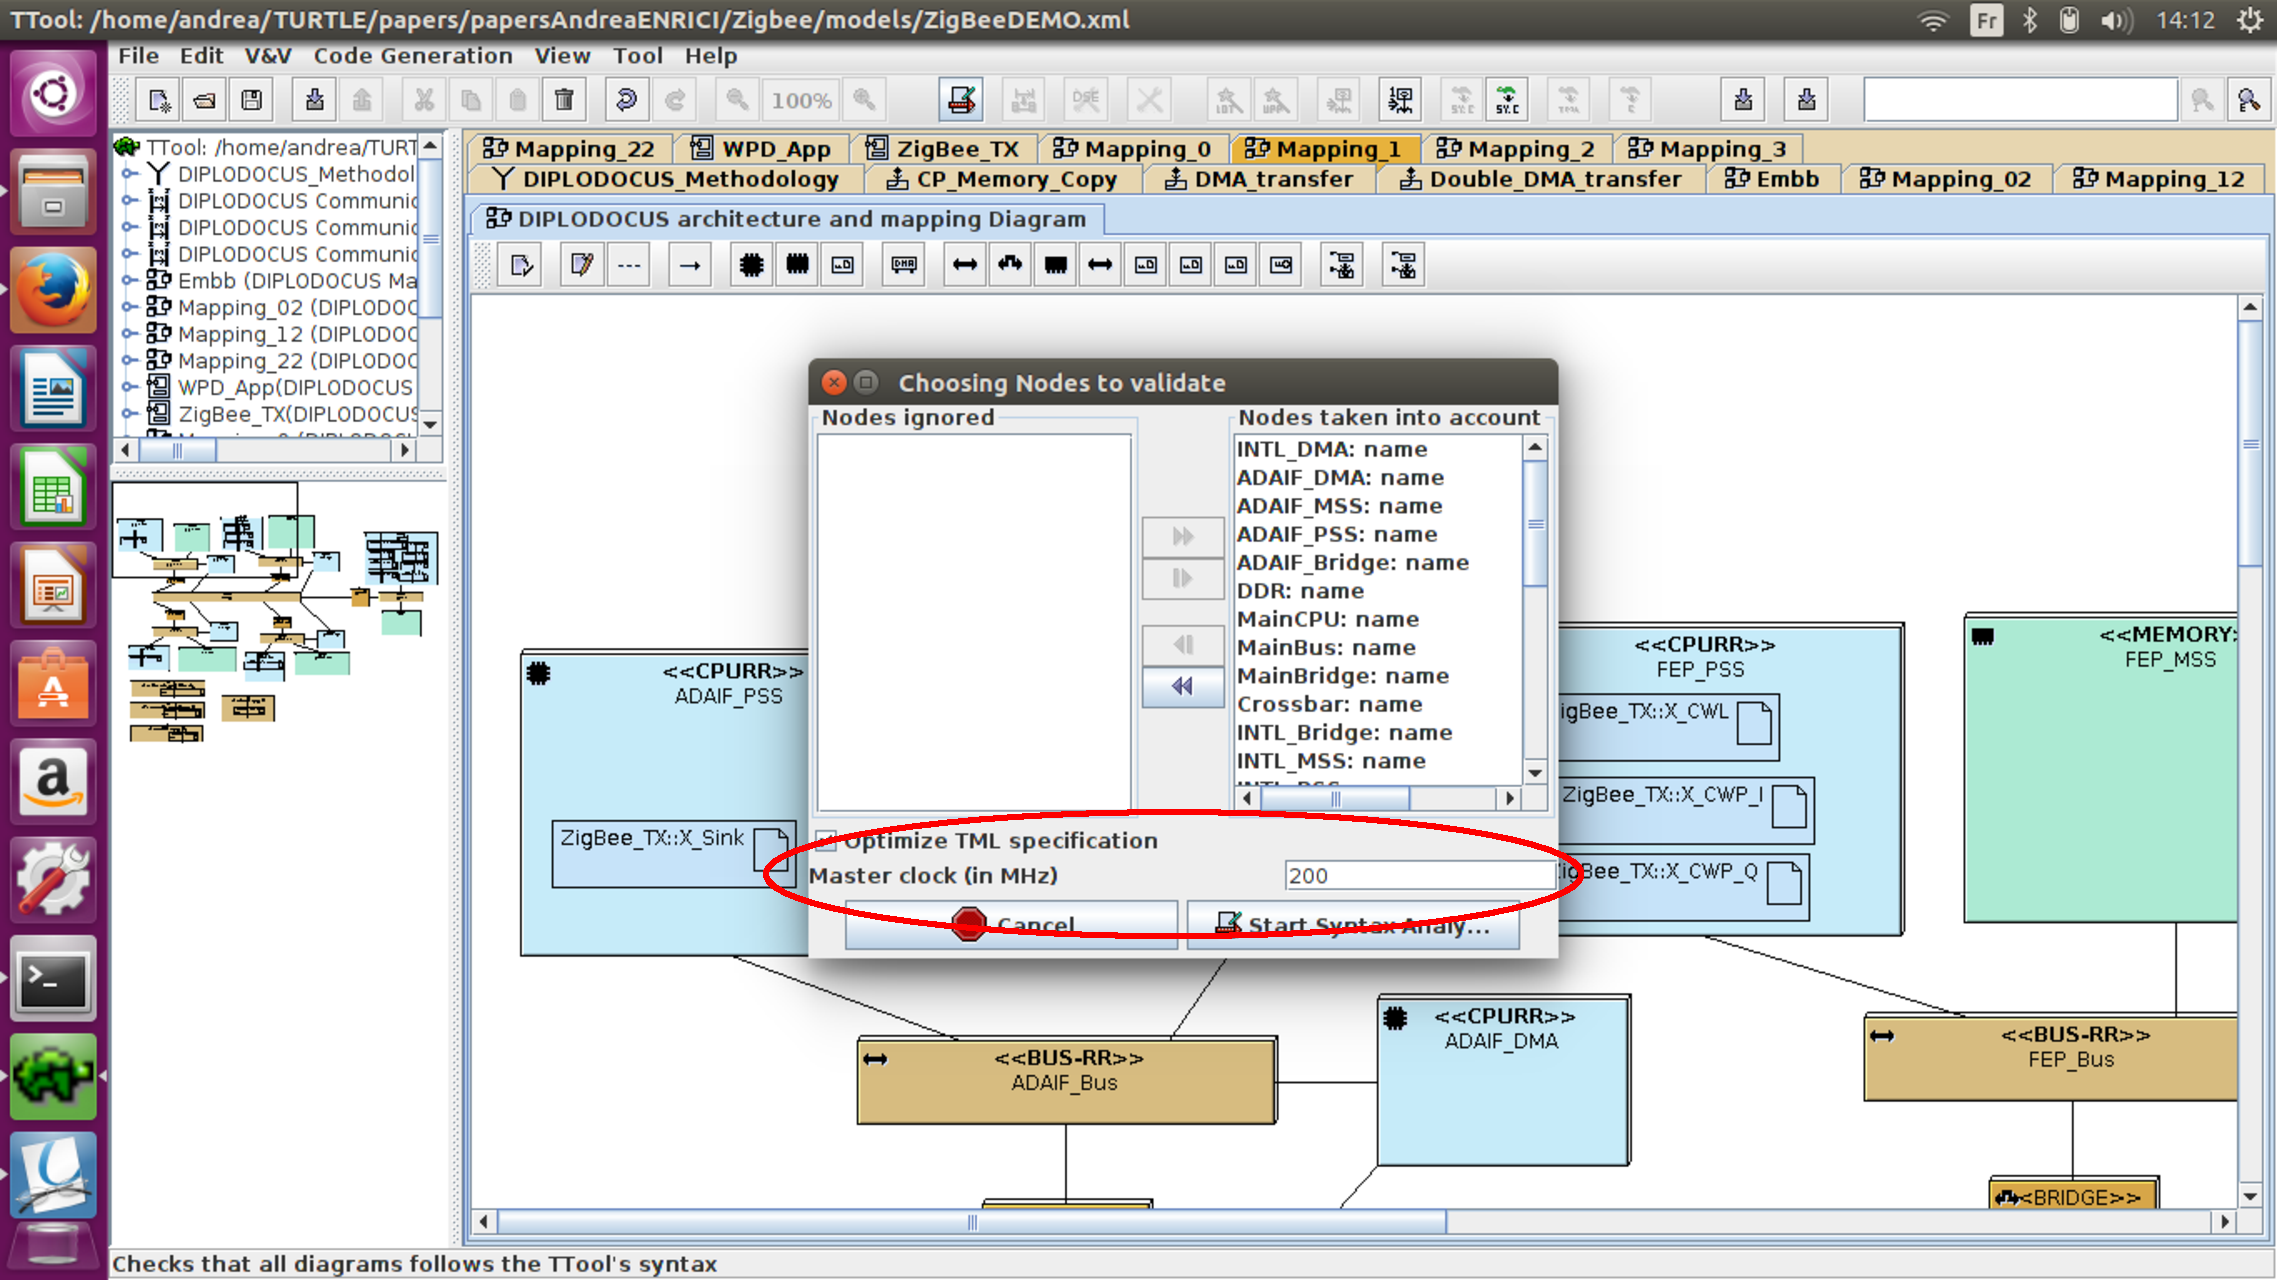
\includegraphics[width=\screenshotsize]{figures/screenshot/ClockFrequency.pdf}
	\caption{The Master clock frequency can be input from the syntax analysis window of a mapping diagram}
	\label{fig:ClockFrequency}
\end{figure}
%
Therefore, in the case of EMBB being implemented in an integrated circuit, the Master clock frequency must be set to
1000 (MHz) and the Clock divider of each CPU unit must be set to 1. In the case of EMBB being implemented on a
prototyping board, the Master clock frequency must be set to 100 (MHz), the Clock divider of the PSS of each DSP unit
(modeled as a CPU block) must be set to 1 and the Clock divider of the main CPU must be set to 6. Only natural numbers can
be assigned to the Clock divider parameter.
%
%
%
\newpage
\subsection{Communication protocols and patterns modeling}
\label{subsec:CP}
%
The introduction of separate models dedicated to designing communication protocols and patterns in the
Y-chart approach, Fig.~\ref{fig:Ychart}, results into the $\Psi$ chart approach, Fig.~\ref{fig:Tchart}. This
introduction aims at solving the \textit{communication mismatch} issue. The latter occurs when mapping communications in
the Y-chart (step 2 in Fig.~\ref{fig:Ychart}), due to a \textit{mismatch} between the description of communications
contained in the application and in the architecture models. This mismatch involves, on one hand, the primitives and
operational semantics used to describe communications in the application model (e.g., point-to-point data channels with
blocking read()/write() operations) and, on the other hand, the primitives and operational semantics used in the
platform model (e.g., configuring and executing a DMA data transfer or a series of bus transactions).
%
\begin{figure}[htbp]
	\centering
	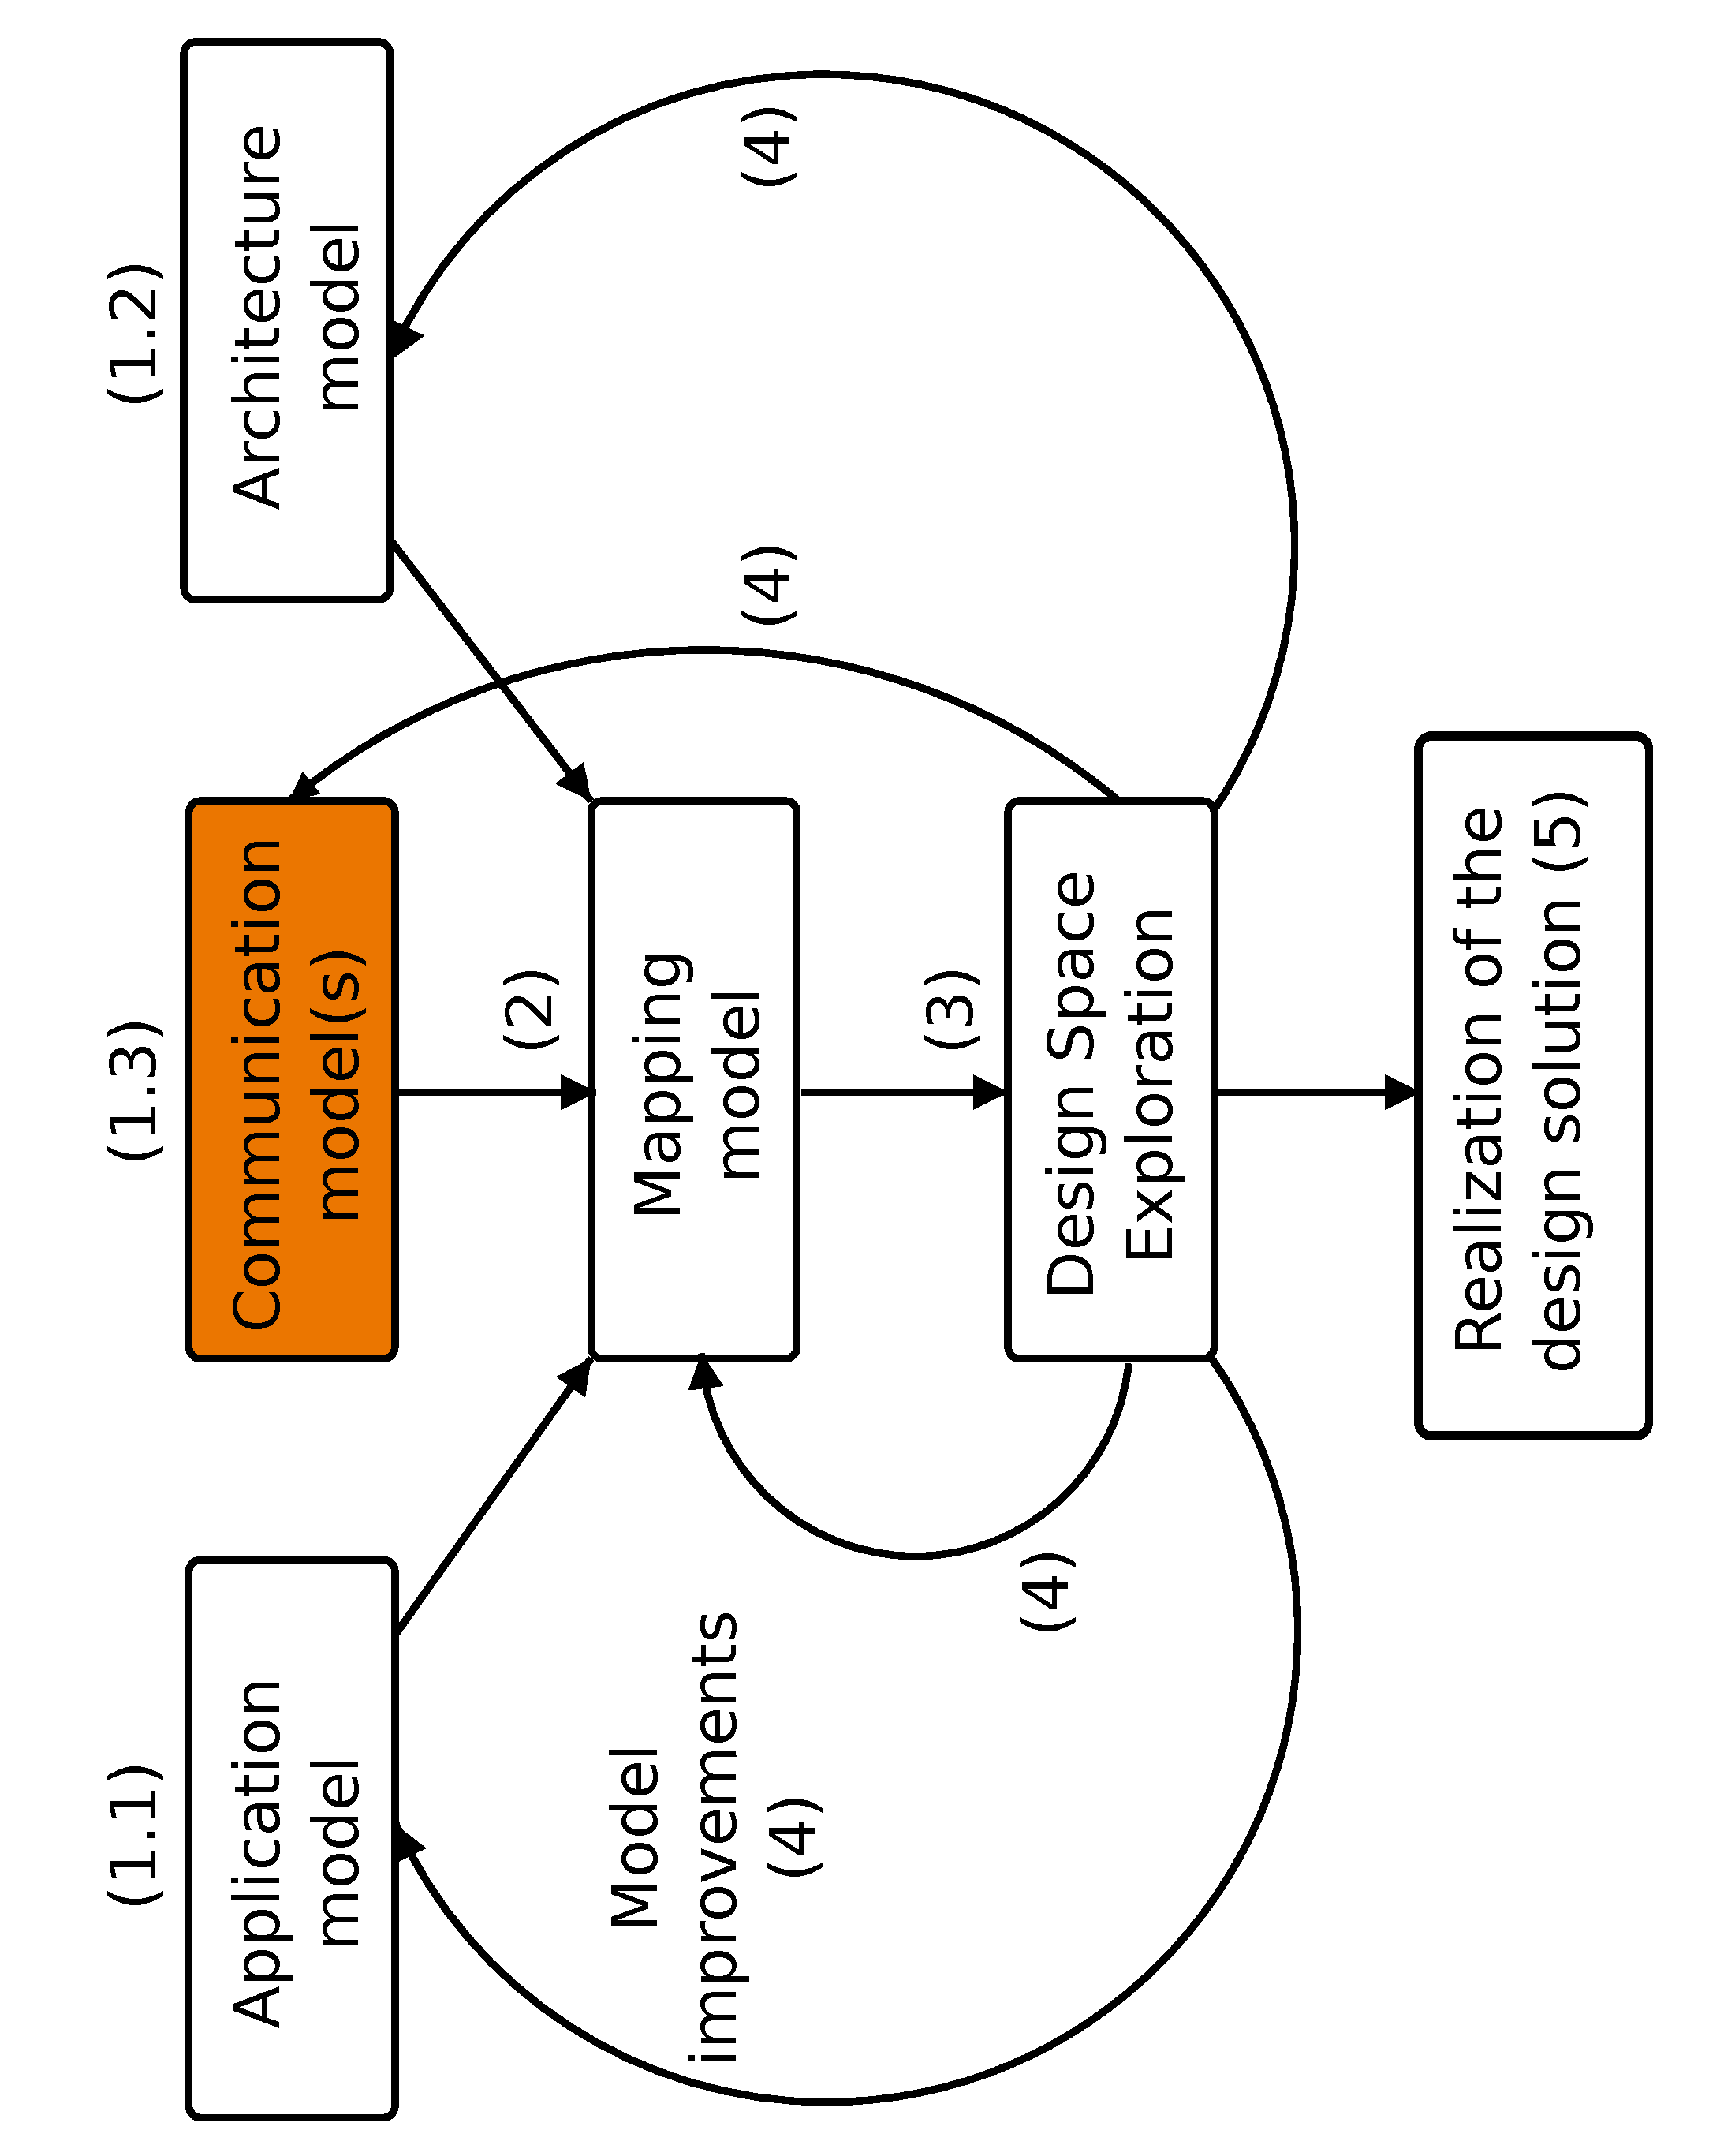
\includegraphics[angle=-90,origin=c,width=0.4\textwidth]{figures/PsiChartCom.pdf}
	\caption{The communication model step, that is described in this section, in the context of the $\Psi$-chart design
    approach}
	\label{fig:PsiChartCom}
\end{figure}
%
\\The communication models of the $\Psi$-chart that we implemented for TTool/\-DI\-PLO\-DO\-CUS are called
Communication Patterns (CPs). These models describe communication protocols at the data-link layer of the ISO/OSI
reference model~\cite{Zimmermann80}. CPs are deployed to model communication protocols at Electronic System-Level of
abstraction. Therefore, CPs do not consider the effects of caching on communications (e.g., the transfers between a
cache and main memory due to a cache miss) that occur at a micro-architecture level of abstraction. Caching effects are
abstracted in the timing attributes of a generic CPU block in the platform model. An attribute, called
\textit{cache-miss ratio}, is used by the DSE engine of TTool/DIPLODOCUS as a penalty that is associated to each
read/write operation between generic CPUs and memory blocks of the platform model.\\
%
A Communication Pattern describes the \emph{behavior} of a communication protocol, intended as a set of rules for the
exchange of data between \emph{components} of an embedded system. A component is intended as a generic architecture
unit, regardless its implementation, i.e., hardware, software or both.\\
%
According to the communication services offered by EMBB, information can be transferred via bus transactions, DMA
transactions or via CPU load/store operations (CPU memory-copy). In the next paragraphs, we show the models that we
created for these transfer mechanisms. We remind to the reader that a CP is denoted with a main SysML Activity Diagram
that describes the algorithm of a communication protocol/pattern. This diagram, in turn, references other SysML Activity
Diagrams or UML Sequence Diagrams. The UML Sequence Diagram for a CP is used to model interactions (e.g., signals)
between actors of a communication protocol (e.g., master , slave). These actors are represented as UML instances. Each
instance has a set of unique attributes (e.g., integer, boolean variables) and can exchange synchronous parameterized
messages with other instances. Instances belong to 3 different types: transfer, control and storage. Transfer instances
(e.g., they denote a bus) can only forward messages, storage instances (e.g., they denote a memory) can only receive
messages and control instances (e.g., they denote a CPU) can both send and receive messages.\\
%
For the interested reader, Appendix~\ref{app:FormalCP} provides a more formal description of Communication Patterns and
of all their properties and semantics.\\
%
Last but not least, TTool cannot currently analyze models of communication patterns. As a consequence, \textbf{communication patterns can be used for documentation purpose only}. Yet, TTool internally understands three CPs: "DMA", "double DMA" and "MemoryCopy". The identification of these patterns is made according to their NAMING, as given in the code of the tmltranslator.TMLCPLib.java source file:
\begin{lstlisting}
public boolean isDMATransfer() {
        return typeName.compareTo("DMA_transfer") == 0;
}

public boolean isDoubleDMATransfer() {
        return typeName.compareTo("Double_DMA_transfer") == 0;
}

public boolean isMemoryCopy() {
        return typeName.compareTo("CP_Memory_Copy") == 0;
}
\end{lstlisting}
Finally, whatever the content of the communication pattern, what is currently relevant for TTool is the name of the communication pattern.

%
%
\subsection{Modeling a DMA data transfer with Communication Patterns}
\label{subsec:CPExample}
%
In this subsection we illustrate how our Communication Patterns can be deployed to model the communication protocol of a
generic data transfer via DMA. We first show the Communication Pattern modeling
an interrupt-based DMA transfer, where the transfer completion is signaled by the DMA controller with an interrupt to the CPU. Next, we present a Communication
Pattern where the CPU polls the DMA controller to detect the transfer completion.\\

The main Activity Diagram of the Communication Pattern for the interrupt-based transfer is illustrated in
Fig.~\ref{fig:CPforDMA}. In this diagram we decomposed the communication protocol into three steps (Sequence Diagrams):
first the data transfer is configured (ConfigureDMA\_SD in
Fig.~\ref{fig:CPforDMA}), then data are iteratively transferred (DMACycle\_SD in
Fig.~\ref{fig:CPforDMA}) and the data transfer is terminated (TerminateDMA\_SD in Fig.~\ref{fig:CPforDMA}). Data are transferred iteratively, as expressed by the $iteration$ operator, based on the value
assigned to the control variable {\tt counter} during the initialization phase.
%
\begin{figure}[!htbp]
	\centering
	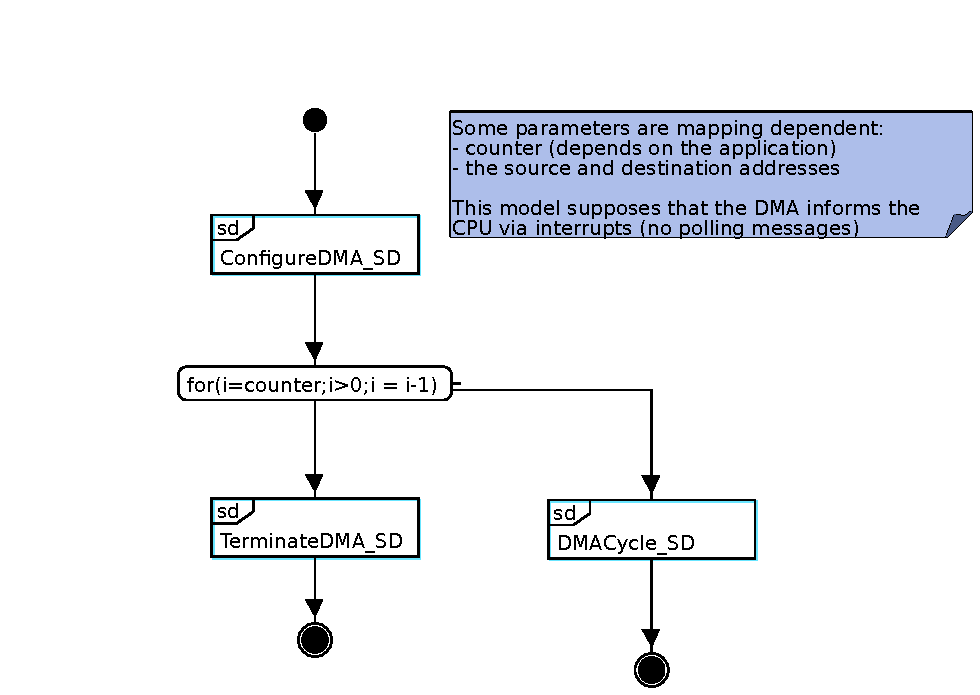
\includegraphics[width=0.7\textwidth]{figures/mainAD_DMA_noPolling.pdf}
	\caption{The main Activity Diagram of a Communication Pattern modeling a data transfer via DMA. In this case,
        interrupts are used as a communication mechanism to notify the transfer completion.}
	\label{fig:CPforDMA}
\end{figure}
%

The Sequence Diagram ConfigureDMA\_SD is depicted in
Fig.~\ref{fig:ConfigureDMA_SD}. Here, we model how a generic CPU unit configures the DMA controller for a data transfer. These two units are represented as two instances of type controller,
interconnected by an instance of type transfer. The CPU instance sends the source and destination addresses ({\tt
sourceAddress}, {\tt destinationAddress}) and the amount of data to transfer ({\tt counter}) as parameters of the
message {\tt TransferRequest()} to the DMA controller, via the transfer instance. The DMA controller, upon reception of
the message, retrieves the parameters and sets an internal counter ({\tt counter}) whose value is equal to the amount of
data to transfer. At this point, it is important to remark that all message parameters are not initialized as our
Communication Patterns are independent of the application model. It is in fact the application model that expresses
the numerical value of the exact amount of data that must be transferred. Similarly, the exact value of the source and
destination addresses depends on the units of the platform model where the CP is mapped. This missing information will
be added to the models only during the mapping phase.
%
\begin{figure}[!htbp]
	\centering
	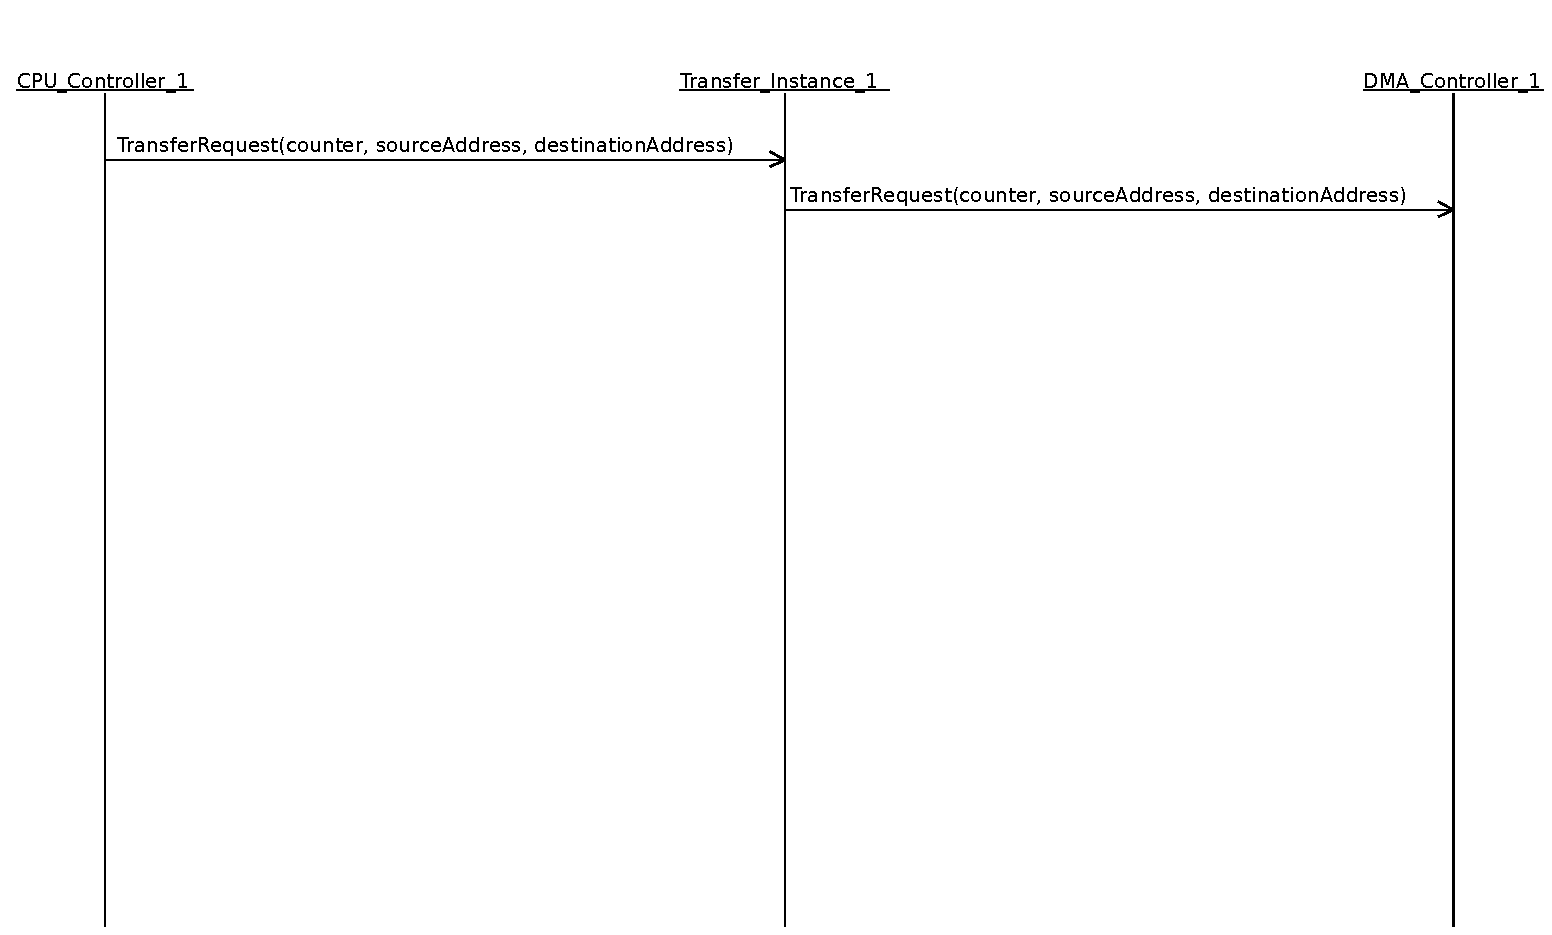
\includegraphics[trim= 0cm 12cm 0cm
0cm, clip, width=\textwidth]{figures/ConfigureDMA_SD.pdf}
	\caption{The Sequence Diagram ConfigureDMA\_SD of Fig.~\ref{fig:CPforDMA}.}
	\label{fig:ConfigureDMA_SD}
\end{figure}
%

In the Sequence Diagram DMACycle\_SD of Fig.~\ref{fig:DMACycle_SD}, we model
one DMA transfer cycle. For this purpose we instantiate the DMA controller of Fig.~\ref{fig:ConfigureDMA_SD}, a source and destination storage instances and two transfer instances. The latter are used to interconnect the DMA controller to the two storage instances. The transfer
cycle is modeled with the DMA controller reading samples out of the source
storage component via a parametrized {\tt Read()} message, where {\tt size} indicates the amount of data that is read. Next, the DMA controller writes data to the
destination storage via a {\tt Write()} message and decrements the counter.
Similarly to the above diagrams, we note here that parameters {\tt size}, {\tt sourceAddress} and {\tt destinationAddress} depend on the system's architecture
and are therefore left as unspecified. They will be assigned a value after the instances are mapped onto a specific DMA
and memory units as detailed in subsection~\ref{subsec:Mapping}. The message parameter \texttt{size} defines the amount
of data that the channel of the DMA controller is able to transfer at each transfer-cycle.
%
\begin{figure}[!htbp]
	\centering
	\includegraphics[trim= 0cm 10cm 0cm 0cm, clip,
	width=\textwidth]{figures/DMACycle_SD.pdf}
	\caption{The Sequence Diagram DMACycle\_SD of Fig.~\ref{fig:CPforDMA}.}
	\label{fig:DMACycle_SD}
\end{figure}
%

In the last Sequence Diagram TerminateDMA\_SD of Fig.~\ref{fig:TerminateDMA_SD},
the DMA controller sends an acknowledgment message ({\tt TransferTerminated()}) to the CPU controller to inform the latter that the transfer has
terminated. One last point that we want to highlight is that all the above-mentioned transfer instances (i.e.,
TransferInstance\_1-4) are different objects of the same instance class (i.e., $transfer$). As a matter of fact, at this
level of abstraction we have no information about the physical route that is used to transfer information in the target
platform.\\
%
\begin{figure}[!htbp]
	\centering
	\includegraphics[trim= 0cm 12.5cm 0cm 0cm,
	clip, width=0.7\textwidth]{figures/TerminateDMA_SD.pdf}
	\caption{The Sequence Diagram TerminateDMA\_SD of Fig.~\ref{fig:CPforDMA}.}
	\label{fig:TerminateDMA_SD}
\end{figure}
%

Fig.~\ref{fig:CPforPollingDMA} shows the main Activity Diagram of a Communication Pattern where the CPU polls the DMA
controller in order to detect the termination of the data transfer. In this case, we modeled the communication protocol
with one Sequence Diagram, ConfigureTransfer and two Activity Diagrams: TransferCycleAD and PollingCycleAD. Similarly to
the Communication Pattern of Fig.~\ref{fig:CPforDMA}, we first model the configuration of the data transfer with a
Sequence Diagram, ConfigureTransfer. Next, we model the transfer cycle and the polling cycle being executed in parallel.
These two phases cannot be modeled directly with Sequence Diagrams as they
require the description of a set of interactions that are iteratively executed.

\begin{figure}[!htbp]
	\centering
	\includegraphics[width=3in]{figures/mainCPDMAPolling.pdf}
	\caption{The main Activity Diagram of the Communication Pattern modeling the data transfer via DMA. In this case,
        polling is used as a mechanism to notify the transfer termination.}
	\label{fig:CPforPollingDMA}
\end{figure}

The Sequence Diagram ConfigureTransfer of Fig.~\ref{fig:ConfigureTransferPolling} is similar to the one described in
Fig.~\ref{fig:ConfigureDMA_SD}: the only difference is the initialization of the flag {\tt transferTerminated} to false. The
latter is set to true by the DMA controller upon termination of the data transfer.

\begin{figure}[!htbp]
	\centering
	\includegraphics[trim= 0cm 11cm 0cm 0cm,
	clip, width=\textwidth]{figures/ConfigureTransferPolling.pdf}
	\caption{The Sequence Diagram ConfigureTransfer of Fig.~\ref{fig:CPforPollingDMA}.}
	\label{fig:ConfigureTransferPolling}
\end{figure}

Fig.~\ref{fig:TransferCycleAD} depicts the Activity Diagram TransferCycleAD where the Sequence Diagram DMACycle\_SD
is iteratively executed as long as the control variable {\tt counter} is greater than zero, meaning that there are still
data to be transferred. Once all data have been transferred, the DMA controller sets the flag {\tt transferTerminated}
to true in Sequence Diagram EnableFlag. Diagram DMACycle\_SD is not illustrated here as it is the same as diagram
DMACycle\_SD of Fig.~\ref{fig:DMACycle_SD}.

\begin{figure}[!htbp]
	\centering
	\includegraphics[width=2in]{figures/TransferCycleAD.pdf}
	\caption{The Activity Diagram TransferCycleAD of Fig.~\ref{fig:CPforPollingDMA}.}
	\label{fig:TransferCycleAD}
\end{figure}

Fig.~\ref{fig:ADPollingCycle} shows the Activity Diagram PollingCycleAD, where Sequence Diagram PollingCycleSD models
the iterative polling of the DMA controller. This scenario is depicted in Fig.~\ref{fig:SDPollingDMA} where the CPU
intermittently polls the state of the data transfer via a {\tt PollingRequest()} message to the DMA controller until the
message parameter {\tt transferTerminated} is set to true. The exact value of variable {\tt waiting\_time} is left as
unspecified as it depends on the mapping.

\begin{figure}[!htbp]
	\centering
	\includegraphics[width=3in]{figures/PollingCycleAD.pdf}
	\caption{The Activity Diagram PollingCycleAD of
	Fig.~\ref{fig:CPforPollingDMA}.}
	\label{fig:ADPollingCycle}
\end{figure}

\begin{figure}[!htbp]
	\centering
	\includegraphics[trim= 0cm 9cm 0cm 0cm,
	clip, width=0.8\textwidth]{figures/PollingCycleSD.pdf}
	\caption{The Sequence Diagram PollingCycleSD describing the message exchanges of the polling cycle of Fig.~\ref{fig:ADPollingCycle}.}
	\label{fig:SDPollingDMA}
\end{figure}

\subsection{Communication models}

Given the communication resources and services that are available in EMBB, the communications protocols that we need to model are
based on DMA transfers with interrupt mechanisms. The models for a DMA transfer have already been illustrated in the
previous paragraph and therefore we will not repeat their diagrams here.\\
%
With respect to these models, another novel Communication Pattern that we need for the ZigBee transmitter is the one depicted in
Fig.~\ref{fig:MemoryCopy}. Here, the main Activity Diagram captures a memory
copy transfer. This transfer is used in the context of EMBB to model a data transfer from the \texttt{MainMemory} to the local memory of any DSP unit, via a store operation issued by
the \texttt{MainCPU}. Fig.~\ref{fig:MemoryCopy_TransferCycle} displays the Activity Diagram \texttt{TransferCycle}, which models
the message exchanges similarly to the diagram in Fig.~\ref{fig:DMACycle_SD}. Attribute \texttt{numData} specifies the number of
data that are transferred at each cycle.
%The only difference between the \texttt{TransferCycle} diagram of Fig.~\ref{fig:DMACycle_SD} and the one in
%Fig.~\ref{fig:MemoryCopy_TransferCycle} is that the amount of data being transferred in each cycle is fixed to 1 sample.\\
%
Another novel Communication Pattern that we used in our case study is the one illustrated in Fig.~\ref{fig:DoubleDMATransfer}.
This CP captures a pair of sequential DMA transfers and can be used to model a copy operation from one source storage to two
different destination storages.\\
%
The main Activity Diagram of this Communication Pattern is simply composed of two references to Activity Diagrams, composed via
the sequence operator. These references point to the Activity Diagrams of Fig.~\ref{fig:DMATransfer1} and~\ref{fig:DMATransfer2}
that describe a standard DMA transfer as the one presented above in Fig.~\ref{fig:CP04_1}-Fig.~\ref{fig:CP04_6}.
%In order not to repeat diagrams that have already been displayed and described in Chapter~\ref{ch:psiChart}, in this subsection
%we do not show the Sequence Diagrams for the double DMA transfer.
%
%The above-referenced Communication Patterns constitute the \textbf{library of communication models} we will use at mapping level.
%
\begin{figure}[!htbp]
	\centering
	\includegraphics[height=7cm]{figures/evaluation/MemCopy.pdf}
    \caption{The Communication Pattern for a memory copy data-transfer}
	\label{fig:MemoryCopy}
\end{figure}
%
\begin{figure}[!htbp]
	\centering
	\includegraphics[width=\textwidth]{figures/evaluation/MemCopy_TransferCycle.pdf}
    \caption{The Sequence Diagram TransferCycle referenced in Fig.~\ref{fig:MemoryCopy}}
	\label{fig:MemoryCopy_TransferCycle}
\end{figure}
%
\begin{figure}[!htbp]
	\centering
	\includegraphics[height=5cm]{figures/evaluation/DoubleDMATransfer.pdf}
  \caption{The Communication Pattern for a pair of sequential DMA transfers}
	\label{fig:DoubleDMATransfer}
\end{figure}
%
\begin{figure}[!htbp]
	\centering
	\includegraphics[height=7cm]{figures/evaluation/DMATransfer1.pdf}
  \caption{The Activity Diagram referenced by DMATransfer1 in Fig.~\ref{fig:DoubleDMATransfer}}
	\label{fig:DMATransfer1}
\end{figure}
%
\begin{figure}[!htbp]
	\centering
	\includegraphics[height=7cm]{figures/evaluation/DMATransfer2.pdf}
  \caption{The Activity Diagram referenced by DMATransfer2 in Fig.~\ref{fig:DoubleDMATransfer}}
	\label{fig:DMATransfer2}
\end{figure}
%
\begin{figure}[!htbp]
	\centering
	\includegraphics[width=5in]{figures/evaluation/ConfigureTransfer1.pdf}
	\caption{The Sequence Diagram ConfigureDMA\_SD1 of Fig.~\ref{fig:DMATransfer1}.}
	\label{fig:CP04_1}
\end{figure}
%
\begin{figure}[!htbp]
	\centering
	\includegraphics[width=\textwidth]{figures/evaluation/TransferCycleSD1.pdf}
	\caption{The Sequence Diagram DMACycle\_SD1 of Fig.~\ref{fig:DMATransfer1}.}
	\label{fig:CP04_2}
\end{figure}
%
\begin{figure}[!htbp]
	\centering
	\includegraphics[width=5in]{figures/evaluation/TerminateTransfer1.pdf}
	\caption{The Sequence Diagram TerminateDMA\_SD1 of Fig.~\ref{fig:DMATransfer1}.}
	\label{fig:CP04_3}
\end{figure}
%
\begin{figure}[!htbp]
	\centering
	\includegraphics[width=5in]{figures/evaluation/ConfigureTransfer2.pdf}
	\caption{The Sequence Diagram ConfigureDMA\_SD2 of Fig.~\ref{fig:DMATransfer2}.}
	\label{fig:CP04_4}
\end{figure}
%
\begin{figure}[!htbp]
	\centering
	\includegraphics[width=\textwidth]{figures/evaluation/TransferCycleSD2.pdf}
	\caption{The Sequence Diagram DMACycle\_SD2 of Fig.~\ref{fig:DMATransfer2}.}
	\label{fig:CP04_5}
\end{figure}
%
\begin{figure}[!htbp]
	\centering
	\includegraphics[width=5in]{figures/evaluation/TerminateTransfer2.pdf}
	\caption{The Sequence Diagram TerminateDMA\_DMA2 of Fig.~\ref{fig:DMATransfer2}.}
	\label{fig:CP04_6}
\end{figure}
%In this paragraph we present the model of a generic DMA transfer modeled with CPs. The main Activity Diagram of the
%Communication Pattern is illustrated in Fig.~\ref{fig:Merge1}a. In this diagram we decomposed the communication protocol
%in three Sequence Diagrams: first the data transfer is configured (ConfigureTransfer in Fig.~\ref{fig:Merge1}a), then
%data are transferred (TransferCycle in Fig.~\ref{fig:Merge1}a) and the data transfer is terminated (TerminateTransfer in
%Fig.~\ref{fig:Merge1}a). Data are transferred iteratively, as expressed by the for-loop operator, based on the value
%assigned to the control variable {\tt counter} in diagram ConfigureTransfer.\\
%%
%\begin{figure}[!htbp]
%	\centering
%	\includegraphics[width=\textwidth]{figures/Merge1.pdf}
%	\caption{The main Activity Diagram of a DMA data transfer (a), Sequence Diagram ConfigureTransfer (b).}
%	\label{fig:Merge1}
%\end{figure}
%%
%The Sequence Diagram ConfigureTransfer is depicted in Fig.~\ref{fig:Merge1}b. Here, we model how a generic CPU unit
%configures the DMA controller unit. These two units are represented as two instances of type controller, interconnected
%by an instance of type transfer. The CPU instance sends the source and destination addresses as well as the amount of
%data to transfer as parameters of the message {\tt TransferRequest()} to the DMA controller, via the transfer
%instance. The DMA controller, upon reception of the message, assigns variable \texttt{dataToTransfer} to
%\texttt{counter}. The value of these variables is not known at modeling phase as CPs are independent of the data
%dependencies in the application model. A value will be assigned at mapping phase, step L1 in
%Fig.~\ref{fig:MappingMeth}.\\
%%
%In the Sequence Diagram of Fig.~\ref{fig:DMACycle_SD}, TransferCycle, we model one DMA transfer cycle. For this purpose
%we instantiate the DMA controller of Fig.~\ref{fig:Merge1}b, a source and destination storage instances interconnected
%by two transfer instances. In this diagram, the DMA controller reads samples out of the source storage instance via a
%parameterized {\tt Read()} message. Subsequently, it writes data to the destination storage instance via a {\tt Write()}
%message. As the values of parameters {\tt size}, {\tt sourceAddress} and {\tt destinationAddress} depend on the
%architecture units, they will be assigned a value when mapping the instances onto DMA and memory units as described in
%subsection~\ref{subsec:Mapping}. Parameter \texttt{size} defines the amount of data that the DMA channel
%transfers each transfer cycle.
%%
%\begin{figure}[!htbp]
%	\centering
%	\includegraphics[width=0.7\textwidth]{figures/DMACycle_SD.pdf}
%	\caption{The Sequence Diagram TransferCycle of Fig.~\ref{fig:Merge1}a.}
%	\label{fig:DMACycle_SD}
%\end{figure}
%%
%\\In the Sequence Diagram TerminateTransfer of Fig.~\ref{fig:Merge1}a, the DMA controller informs the CPU instance that
%the transfer is terminated via an acknowledgment message.
%%
%\subsubsection{Modeling a CPU memory-copy operation with Communication Patterns}
%%
%Another communication mechanism that we need to model in the frame of the ZigBee case study is the CPU memory-copy
%operation. The corresponding Communication Pattern is shown in Fig.~\ref{fig:Merge2}a. Here, the main Activity Diagram
%captures a memory copy transfer that is used in Embb to move data from the \texttt{MainMemory} to the local memory of
%any DSP unit, via a store operation issued by the \texttt{MainCPU}. The Sequence Diagram \texttt{TransferCycle} in
%Fig.~\ref{fig:Merge2}a, models the message exchanges in the same way as the diagram in Fig.~\ref{fig:DMACycle_SD}, except
%for the decrement of attribute \texttt{counter}.\\
%%
%\subsubsection{Composing Communication Patterns}
%%
%In this paragraph we briefly illustrate how CPs can be composed to model more complex patterns. The CP in
%Fig.~\ref{fig:Merge2}b captures a pair of sequential DMA transfers and can be used to describe a copy operation from
%one source storage to two different destination storages. The main Activity Diagram of this CP is composed of two
%references to Activity Diagrams, that each describe a DMA transfer as the one illustrated in Fig.~\ref{fig:Merge2}c for
%DMATransfer1 that is a copy of the one in Fig.~\ref{fig:Merge1}.
%%
%\begin{figure}[!htbp]
%	\centering
%	\includegraphics[width=\textwidth]{figures/Merge2.pdf}
%	\caption{The main AD for a CP modeling a CPU memory copy (a). The main AD for a CP modeling the sequence of two DMA
%	transfers (b). Part (c) shows the AD referenced by DMATransfer1 in (b).}
%	\label{fig:Merge2}
%\end{figure}
%
\subsubsection{The communication mismatch in EMBB}
%
In the application and platform models that we presented so far, we remind the reader that communications are
described in terms of:
%
\begin{itemize}
	\item Point-to-point unidirectional data-channels between tasks of the application model. A task accesses these
        channels via: (i) blocking read/blocking write, (ii) blocking read/non-blocking write, (iii) non-blocking
        read/non-blocking write operations.
	%
	\item Read/write operations performed by processing units (i.e., CPU, Hardware Accelerator, HwA) to/from memory
        units in the architecture model. CPU units and HwA units issue read and write requests over bus and bridge
        units. As described in~\cite{Knorreck11}, buses may be endowed with several independent communication channels
        which can be used simultaneously. The communication between architecture units makes use of the circuit
        switching paradigm: during the entire data transmissions on more than one bus, at least one communication
        channel on all involved buses has to be available and is reserved. Reservation is accomplished starting from the
        CPU towards the memory element in causal fashion.
\end{itemize}
%
Given the semantics of an application and platform models in TTool\-/DI\-PLO\-DO\-CUS, communication mismatches arise
when data are transferred via paths in the platform model that encompass a sequence of more than one bus between a
source CPU and a destination memory.\\
%
Specifically to the case study described in this tutorial, communication mismatches arise when data are transferred:
%
\begin{itemize}
	%
	\item from \texttt{MainMemory} to any of the DSP local memories and vice-versa, e.g., path
	\texttt{DDR\--MainBus\--MainBridge\--Crossbar\--MAPPER\_Bridge\--MAPPER\_Bus\--MAPPER\_MSS} in Fig. \ref{fig:CommMismatchesPaths}
	%
	\item from a DSP local memory to any other DSP local memory, e.g., path
	\texttt{MAPPER\_MSS\--MAPPER\_Bus\--MAPPER\_Bridge\--Crossbar\--INTL\_Bridge\--INTL\_Bus\--INTL\_MSS} in Fig. \ref{fig:CommMismatchesPaths}
	%
\end{itemize}
%
The only case in which there is a communication \textit{match} between the application and the platform is given by the
path \texttt{MainCPU-MainBus-MainMemory} or the path that links a DSP PSS to its local memory, e.g.,
\texttt{MAPPER\_\-PSS-MAPPER\_\-Bus-MAPPER\_\-MSS} in Fig.~\ref{fig:CommMismatchesPaths}.
%
\begin{figure}[!htbp]
	\centering
	\includegraphics[angle=-90,origin=c,height=0.8\paperwidth]{figures/evaluation/CommMismatchesPaths.pdf}
  \caption{An excerpt of the platform model of EMBB. In red are highlighted two paths processor\--bus\--memory that are NOT source
	of a communication mismatch when mapping data channels from the application model.}
	\label{fig:CommMismatchesPaths}
\end{figure}
%
\newpage
\subsubsection{Creating Communication Pattern diagrams}
%
To create a Communication Pattern, left click on the panel tab and select \texttt{New Partitioning - Communication
Pattern}, then rename the panel to \texttt{DMAtransfer}. Fig.~\ref{fig:CPWindow1} shows the design window of the main
Activity Diagram of a Communication Pattern and enumerates the available buttons.
%
\begin{figure}[!htbp]
	\centering
	\includegraphics[width=\screenshotsize]{figures/screenshot/CPWindow1.png}
	\caption{The design window for an Activity Diagram of a Communication Pattern}
	\label{fig:CPWindow1}
\end{figure}
%
\begin{enumerate}
	\item Edit Communication Pattern Diagram
	%
	\item Add a comment: add a comment to the diagram
	%
	\item Connector: add a connector between two elements of a diagram
	%
	\item Start: instantiate the start node
	%
	\item Stop: instantiate the stop node
	%
	\item Reference to a SD: instantiate a reference to CP Sequence Diagram
	%
	\item Reference to an AD: instantiate a reference to a CP Activity Diagram
	%
	\item Fork: instantiate the fork operator
	%
	\item Join: instantiate the join operator
	%
	\item Choice: instantiate the choice operator
	%
	\item Loop: instantiate a for-loop operator
	%
	\item Enhance
	%
\end{enumerate}
%
The design window that is automatically created is that of the main Activity Diagram, that is the top-most diagram of a
Communication Pattern. To create an Activity Diagram, that will be referenced by the main diagram, instantiate a reference
to an Activity Diagram (button n.7), right-click on the reference and select \texttt{Create Activity Diagram}. This will
automatically create a diagram whose design window is the same as the one of the main Activity Diagram.
%
To design the main Activity Diagram of the DMA transfer, as illustrated in Fig.~\ref{fig:CPforDMA}, we must instantiate
and interconnect 1 start node, 3 references to Sequence Diagrams, 1 for-loop and 2 stop nodes. For this purpose, simply
click on the corresponding buttons, then place and connect the elements in the design area. To rename a reference to a
Sequence Diagram, double click on it and enter the desired name. To configure the initialization, the termination and
the increment conditions of the for-loop also double click on the for-loop and enter the desired parameters.\\
%
To design diagrams \texttt{ConfigureTransfer}, Fig.~\ref{fig:ConfigureDMA_SD}, \texttt{TransferCycle},
Fig.~\ref{fig:DMACycle_SD}, and \texttt{TerminateDMA\_SD}, Fig.~\ref{fig:TerminateDMA_SD}, right-click on their references,
select \texttt{Open diagram}.\\
%
Fig.~\ref{fig:CPSDWindow1} shows the design window of a CP Sequence Diagram and enumerates the available buttons.
%
\begin{figure}[!htbp]
	\centering
	\includegraphics[width=\screenshotsize]{figures/screenshot/CPSDWindow1.png}
	\caption{The design window for a CP Sequence Diagram}
	\label{fig:CPSDWindow1}
\end{figure}
%
\begin{enumerate}
	\item Edit the Sequence Diagram
	%
	\item Add a comment: add a comment to the diagram
	%
	\item Comment connector
	%
	\item Asynchronous message: instantiate an asynchronous message between a sender and a receiver instances
	%
	\item Storage instance: instantiate an instance of type storage
	%
	\item Controller instance: instantiate an instance of type controller
	%
	\item Transfer instance: instantiate an instance of type transfer
	%
	\item Action state: instantiate an action state for an instance
	%
	\item Align instances: horizontally align multiple instances
	%
\end{enumerate}
%
To design diagram \texttt{ConfigureTransfer}, instantiate 2 controller instances and 1 transfer instance by clicking on
button n.6 and button n.7 (Fig.~\ref{fig:CPSDWindow1}), respectively. Double click on an instance to open the window
that allows us to rename it and to add attributes. Rename the initiator instance as \texttt{CPU\_Controller}, then add
attributes \texttt{counter} of type \texttt{Natural}, \texttt{sourceAddress} and \texttt{destinationAddress} of type
\texttt{Address}. Similarly, rename the receiver controller instance as \texttt{DMA\_Controller} and the transfer
instance as \texttt{TransferInstance\_1}. Before including messages to the diagram, add to these 2 instances the same
attributes as those for the \texttt{CPU\_Controller}. This is important because, given a pair of instances of a Communication
Pattern, $I_1,I_2$, interconnected by message $M$ that carries parameters $P=(p_1,p_2,...p_n)$, the user must define parameters $P$ for both $I_1$ and
$I_2$.\\
%
Now, connect the instances with asynchronous message \texttt{TransferRequest} as shown in Fig.~\ref{fig:ConfigureDMA_SD}. Click
on button n. 4 (Fig.~\ref{fig:CPSDWindow1}) and the tool will highlight (yellow boxes) the connection points along the
lifelines of the available instances. Click on one of these points on a sender instance and then click on a connection
point on a receiver instance. Double click on the message arrow, enter the message name and its parameters.\\
%
To design diagram \texttt{TransferCycle}, instantiate 1 controller instance (named \texttt{DMA\_Controller}), 2 transfer
instances (named \texttt{TransferInstance\_2} and \texttt{TransferInstance\_3}) and 1 storage instance (named
\texttt{SOURCE\_Storage}). Then include messages \texttt{Read()} and \texttt{Write()}, Fig.~\ref{fig:DMACycle_SD}, as
described above for diagram \texttt{ConfigureTransfer}. To add the action state that decrements attribute
\texttt{counter}, click on button n.8 (Fig.~\ref{fig:CPSDWindow1}) and place the action state on a target instance.
Double click the action to enter the action that decrements the counter: \texttt{counter = counter - size}.\\
%
To design diagram \texttt{TerminateDMA\_SD} instantiate 2 controller instances (named \texttt{DMA\_Controller} and
\texttt{CPU\_Controller}) and 1 transfer instance (named \texttt{TransferInstance\_4}). Then interconnect them via
message \texttt{TransferTerminated()} as shown in Fig.~\ref{fig:TerminateDMA_SD}.\\
%

\noindent
To design the Communication Patterns for two serial DMA transfers as in Fig.~\ref{fig:DoubleDMATransfer}, create a new
CP. Add the references to 2 Activity Diagrams, button n.7 in Fig.~\ref{fig:CPWindow1}, and a stop node, button n.5 in
Fig.~\ref{fig:CPWindow1}. Then, simply name the two references \texttt{DMATransfer1} and \texttt{DMATransfer2}. For
each DMA transfer, copy the activity and sequence diagrams that we have just created. Then, assign unique names to the
diagrams, the instances and their attributes as shown in Fig.~\ref{fig:DMATransfer1} - Fig.~\ref{fig:CP04_6}.\\
%
After this point of the tutorial, we let the user design by himself/herself the diagrams for the CPU memory-copy operation
of Fig.~\ref{fig:MemoryCopy}.\\
%
\newpage
\subsection{Mapping}
\label{subsec:Mapping}
%
Fig.~\ref{fig:MappingMeth} details the methodology that we defined in the $\Psi$-chart approach
(Fig.~\ref{fig:PsiChartMap}) in order to create a complete mapping model (step 2 in Fig.~\ref{fig:Tchart}). The mapping
methodology in Fig.~\ref{fig:MappingMeth} shows the process required to \textit{bind} the application and communication
models onto the platform model.
%
\begin{figure}[htbp]
	\centering
	\includegraphics[angle=-90,origin=c,width=0.4\textwidth]{figures/PsiChartMap.pdf}
	\caption{The mapping step that is described in this section, in the context of the $\Psi$-chart design approach}
	\label{fig:PsiChartMap}
\end{figure}
%
\begin{figure}[htbp]
	\centering
	\includegraphics[angle=-90,origin=c,width=0.8\textwidth]{figures/applicationModel1.pdf}
	\vspace{-10em}
	\caption{The mapping methodology of the $\Psi$-chart (left side) and the models for each step (right side).}
	\label{fig:MappingMeth}
\end{figure}
%
\\\textbf{Computation (level L0).}
%
The computational parts of the application model are mapped to the platform model. For instance, a node in the
application MoC that models an FFT operation is mapped to a Digital Signal Processor (DSP) unit; a node modeling a
control task is mapped to a Central Processing Unit (CPU). Similarly, for variables which are dependent on the specific
characteristics of the mapped unit, a value is assigned accordingly. For instance, variables describing abstract data
types (e.g., complex numbers) are assigned a value (e.g., \texttt{cpx32} in case the mapped DSP unit represents complex
numbers with 16 bits for the imaginary part and 16 bits for the real part).\\
%
\textbf{Storage (level L1).}
%
Any behavior and variable in the application model that is related to the storage of data or control information is
mapped. A system engineer selects the platform units (e.g., memories, buffers) that will store the data and/or
control information produced or consumed by the computations mapped at level L0. According to the selected units and
their characteristics, parameters are assigned a value, e.g., the size of a buffer.\\
%
At this point, data dependencies in the application model must be associated to the communication models that describe
the corresponding transfer of data. In our implementation of the $\Psi$-chart in TTool/DIPLODOCUS this is performed by
the user who associates a data channel between computations to a Communication Pattern (sub-section~\ref{subsec:CP}).
We specify that this solution is not imposed by the design principles of the $\Psi$-chart approach. Other types of
relations may be deployed according to the characteristics of the specific design tool into which the $\Psi$-chart
is implemented (e.g., matching signature operations).\\
%
\textbf{Communication configuration (level L2).}
%
The behavior and parameters of a communication model are mapped to the platform model. A system engineer selects the
platform units that will be in charge of configuring the data transfers that move data from the source to the
destination storage units mapped at level L1.\\
%
\textbf{Routing (level L3).}
%
The route that data will take to be transferred between a source and a destination storage is chosen in terms of
transfer units (e.g., bus, bridge) according to the topology of the architecture model.\\
%

%According to the mapping methodology of Fig.~\ref{fig:MappingMeth}, we first map the computations of the application
%model of Fig.~\ref{fig:ZigBeeTX} onto the platform model in Fig.~\ref{fig:Embb}. Such a mapping results in each control
%task (e.g., F\_Symbol2ChipSeq) being executed by the Main CPU unit and the data-processing tasks (e.g.,
%X\_Symbol2ChipSeq) being executed by the DSPUs PSS. Secondly, the memories where to store input/output data are chosen.
%This results into a mapping where the local memory of each DSPU is used to store the input/output data for the
%computations that have been mapped onto the DSP's Processing SubSystem, e.g., task X\_Symbol2ChipSeq is mapped to the
%Mapper PSS, the input/output data are mapped to the Mapper local Memory SubSystem (MSS).\\
%%
%Subsequently, from our library of communication models we instantiate and map 4 Communication Patterns:
%%
%\begin{itemize}
%	\item \textit{CP01}: a memory copy CP that transfers the output data of task X\_Source. It is composed of: 1 controller instance
%	(CPU\_Controller), 2 storage instances (Src\_Storage, Dst\_Storage) and 2 transfer instances.
%	%
%	\item \textit{CP02}: a DMA CP that transfers the output data of X\_Symbol2ChipSeq. It is composed of: 2 controller instances
%	(CPU\_Controller, DMA\_Controller), 2 storage instances (Src\_Storage, Dst\_Storage) and 4 transfer instances.
%	%
%	\item \textit{CP03}: a DMA CP that transfers the output data of X\_Chip2Octet. It is composed of: 2 controller instances
%	(CPU\_Controller, DMA\_Controller), 2 storage instances (Src\_Storage, Dst\_Storage) and 4 transfer instances.
%	%
%	\item \textit{CP04}: the sequence of two DMA CPs that transfer the output data of X\_CWP\_I and X\_CWP\_Q. It is composed of: 4
%	controller instances (2 CPU\_Controllers, 2 DMA\_Controllers), 4 storage instances (2 Src\_Storage, 2 Dst\_Storage) and 8
%	transfer instances.
%\end{itemize}
%%
%The above CPs are mapped onto the units listed in Table I. \hl{Due to lack of space, we do not show the mapping at routing
%level (L3 in Fig.~\ref{fig:MappingMeth}) of the transfer instances. Does this mapping exist somewhere? In the thesis
%maybe}
%%
%\begin{table}[!htbp]
%\centering
%\caption{The mapping of the CPs' controller and storage instances}
%\label{tab:MappingTable}
%\begin{tabular}{| >{\centering\arraybackslash}p{2cm} | >{\centering\arraybackslash}p{4cm} | >{\centering\arraybackslash}p{4cm} |}
%	\hline
%		\textbf{Identifier}	& \textbf{Instance} & \textbf{Architecture unit} \\ \hline
%		\multirow{2}{*}{\textbf{CP01}} & \parbox[t]{4cm}{\centering Src\_Storage,\\Dst\_Storage\\} & \parbox[t]{4cm}{\centering Main
%		Memory\\MAPPER\textsubscript{MSS}\\} \\ \hline
%		%
%		\multirow{3}{*}{\textbf{CP02}} & \parbox[t]{4cm}{\centering DMA\_Controller,\\Src\_Storage,\\Dst\_Storage\\} &
%		\parbox[t]{4cm}{\centering MAPPER\textsubscript{DMA}\\MAPPER\textsubscript{MSS}\\INTL\textsubscript{MSS}\\} \\ \hline
%		%
%		\multirow{3}{*}{\textbf{CP03}} & \parbox[t]{4cm}{\centering DMA\_Controller,\\Src\_Storage,\\Dst\_Storage\\} &
%		\parbox[t]{4cm}{\centering INTL\textsubscript{DMA}\\INTL\textsubscript{MSS}\\FEP\textsubscript{MSS}\\} \\ \hline
%		%
%		\multirow{3}{*}{\textbf{CP04}} & \parbox[t]{4cm}{\centering DMA\_Controllers,\\Src\_Storages,\\Dst\_Storages\\} &
%		\parbox[t]{4cm}{\centering FEP\textsubscript{DMA}\\FEP\textsubscript{MSS}\\ADAIF\textsubscript{MSS}\\} \\ \hline
%		%
%\end{tabular}
%\end{table}
%

\noindent
We describe here the mapping of the application and communication models of the ZigBee transmitter, according to the
methodology in Fig.~\ref{fig:MappingMeth}.\\
%
We first map the computations (level L0) of the application model. As mentioned above, a mapping model is based on an
instance of the platform model. To clone the platform model, right-click on the platform panel, select \texttt{Clone}
then rename the newly copied diagram as \texttt{Mapping}. The mapping of computations is summarized in
Table~\ref{tab:MappingL0}: each control task is mapped on the Main CPU unit and the data-processing tasks are mapped on
the DSPUs. In a design where also the microcontrollers of each DSP unit are deployed, an alternative mapping would be to
delegate some of the control tasks to these local microcontrollers.
%
\begin{table}
\centering
\caption{Computation mapping, level L0}
\label{tab:MappingL0}
\begin{tabular}{| >{\centering\arraybackslash}l | >{\centering\arraybackslash}l | >{\centering\arraybackslash}l |}
	\hline
		\textbf{Task name}		& \textbf{Task type}	&	\textbf{Architecture unit} \\ \hline
		X\_Source							& eXecution			& Main CPU 					\\ \hline
		F\_Source							& Firing				& Main CPU 					\\ \hline
		X\_Symbol2ChipSeq			& eXecution			& Mapper PSS 				\\ \hline
		F\_Symbol2ChipSeq			& Firing 				& Main CPU 					\\ \hline
		X\_Chip\_to\_Octet		&	eXecution 		& Interleaver PSS 	\\ \hline
		F\_Chip\_to\_Octet		&	Firing 				& Main CPU 					\\ \hline
		X\_CWL								&	eXecution 		& FEP PSS 					\\ \hline
		F\_CWL								&	Firing 				& Main CPU 					\\ \hline
		X\_CWP\_I							&	eXecution			& FEP PSS						\\ \hline
		F\_CWP\_I							&	Firing 				& Main CPU 					\\ \hline
		X\_CWL\_Q							&	eXecution 		& FEP PSS						\\ \hline
		F\_CWL\_Q							&	Firing 				& Main CPU 					\\ \hline
		X\_Sink								&	eXecution 		& ADAIF PSS					\\ \hline
		F\_Sink								&	Firing 				& Main CPU 					\\ \hline
\end{tabular}
\end{table}
%
To add the mapping information listed in Table~\ref{tab:MappingL0}, click on the button \texttt{Map a task}\footnote{We
specify here that this button maps a primitive component of the application model. The term \textit{task} is synonymous for a
primitive component of the application model. It is used in the tool for historical reasons as in the TML language, an
application is described in terms of interconnected tasks rather than primitive components (UML/SysML terminology).}
(button n.7 in Fig.~\ref{fig:Platform}) and click on the platform unit where to map the computation. This attaches a UML
artifact to the target platform unit. Double click on the artifact, and in the simulation tab select the task/primitive
component that you want to map, then save and close. To demonstrate, Fig.~\ref{fig:MapSink} shows the mapping of
\texttt{X\_TXsink} on the CPU unit that model the ADAIF computational core.
%
\begin{figure}[htbp]
	\centering
	\includegraphics[width=\screenshotsize]{figures/screenshot/MapSink.png}
	\caption{The mapping of task \texttt{TX\_Xsink} on the ADAIF computational core}
	\label{fig:MapSink}
\end{figure}
%
\\The memories used to store input/output data (mapping level L1) are chosen according to the access capabilities of
each DSPU and of the main CPU. This results in a mapping where the local memory of each DSPU is used to store the
input/output data for the computations that have been mapped onto the DSP's Processing SubSystem. For instance, task
X\_Symbol2ChipSeq is mapped to the Mapper DSPU, therefore, the input/output data are mapped to the Mapper local Memory
SubSystem (MSS). Table~\ref{tab:MappingL1} summarizes this mapping.
%
\begin{table}
\centering
\caption{Storage mapping, level L1}
\label{tab:MappingL1}
\begin{tabular}{| >{\centering\arraybackslash}l | >{\centering\arraybackslash}l | >{\centering\arraybackslash}l |}
	\hline
		\textbf{Task name}		& \textbf{Input data memory} & \textbf{Output data memory} \\ \hline
		X\_Source							& 							& Main memory	\\ \hline
		X\_Symbol2ChipSeq			& Mapper MSS		& Mapper MSS	\\ \hline
		X\_Chip\_to\_Octet		&	INTL MSS			& INTL MSS	\\ \hline
		X\_CWL								&	FEP MSS				& FEP MSS		\\ \hline
		X\_CWP\_I							&	FEP MSS				& FEP MSS		\\ \hline
		X\_CWL\_Q							&	FEP MSS				& FEP MSS		\\ \hline
		X\_Sink								&	ADAIF MSS			& ADAIF MSS	\\ \hline
\end{tabular}
\end{table}
%
To implement the mapping of memory units, we must distinguish between two cases:
\begin{enumerate}
	\item The mapped memory unit is directly connected (i.e., via one single bus unit) to the processing unit where
	the producer task will store its output data. In this case, we have a communication match and no
	Communication Pattern is needed to model the transfer of data. We only need to map a data channel onto a target
	memory: click on button n.14 in Fig.~\ref{fig:Platform}, instantiate the mapping artifact for a data channel onto
    the target memory. Double click on the artifact and select the desired data channel, Fig.~\ref{fig:MapMemory1}, then
    save and close.
	%
	\item The mapped memory unit and the processing unit are not directly connected (i.e., the shortest path between
	the two units is composed of more than one bus). In this case, we are facing a communication mismatch and we
	must instantiate the block dedicated to map a Communication Pattern. Click on button n.12 in
	Fig.~\ref{fig:Platform} and place the block in the mapping model. Then add onto this block the UML artifact to
	map a port, button n.15 in Fig.~\ref{fig:Platform}. Double click on the artifact and select the
	port\footnote{The tool lists the destination ports of each channel} and the memory unit as shown in
	Fig.~\ref{fig:MapMemory2} for the mapping of port chip2octet\_ch\_in onto the local memory of the INTL DSP
	unit.
	%
\end{enumerate}
%
\begin{figure}[htbp]
	\centering
	\includegraphics[width=\screenshotsize]{figures/screenshot/MapMemory1.png}
	\caption{The mapping of a memory unit in absence of a communication mismatch: mapping of a data channel}
	\label{fig:MapMemory1}
\end{figure}
%
\begin{figure}[htbp]
	\centering
	\includegraphics[width=\screenshotsize]{figures/screenshot/MapMemory2.png}
	\caption{The mapping of a memory unit in presence of a communication mismatch: mapping a memory unit via the
	mapping block for Communication Patterns}
	\label{fig:MapMemory2}
\end{figure}
%
At this point, the mapping of the application model is completed and we can proceed to map the Communication Patterns
from our library. For this purpose, we must first decide how data is transferred between DSPUs. Given the mapping of
computations in table~\ref{tab:MappingL0}, EMBB's topology and the expertise of a platform programmer from our research
group, we choose to use:
%
\begin{itemize}
	\item The Main CPU to copy input samples to the Mapper DSPU
	\item The DMA engine of the Mapper to transfer chip sequences to the Interleaver
	\item The DMA engine of the Interleaver to transfer octets to the Front End Processor
	\item The DMA engine of the Front End Processor to transfer samples to the ADAIF
\end{itemize}
%
Therefore, from our library we instantiate and map 4 Communication Patterns:
%
\begin{itemize}
	\item \textit{CP01}: a memory copy CP that transfers the output data of task X\_Source. It is composed of: 1
	controller instance (CPU\_Controller), 2 storage instances (Src\_Storage, Dst\_Storage) and 2 transfer
	instances.
	%
	\item \textit{CP02}: a DMA CP that transfers the output data of X\_Symbol2ChipSeq. It is composed of: 2
	controller instances (CPU\_Controller, DMA\_Controller), 2 storage instances (Src\_Storage, Dst\_Storage) and 4
	transfer instances.
	%
	\item \textit{CP03}: a DMA CP that transfers the output data of X\_Chip2Octet. It is composed of: 2 controller
	instances (CPU\_Controller, DMA\_Controller), 2 storage instances (Src\_Storage, Dst\_Storage) and 4 transfer
	instances.
	%
	\item \textit{CP04}: the sequence of two DMA CPs that transfer the output data of X\_CWP\_I and X\_CWP\_Q. It is
	composed of: 4 controller instances (2 CPU\_Controllers, 2 DMA\_Controllers), 4 storage instances (2
	Src\_Storage, 2 Dst\_Storage) and 8 transfer instances.
\end{itemize}
%
The above CPs are summarized also in Table~\ref{tab:CPList2} and Table~\ref{tab:CPList3}. In the latter, the
\textit{transfer} instances of CP01 are those shown in the diagram in Fig.~\ref{fig:MemoryCopy_TransferCycle}. The
\textit{transfer} instances of CP02 and CP03 are those shown in the Sequence Diagrams of Fig.~\ref{fig:ConfigureDMA_SD},
Fig.~\ref{fig:DMACycle_SD} and Fig.~\ref{fig:TerminateDMA_SD}. We remind the reader (Property 17 in
Appendix~\ref{app:FormalCP}) that the name of an instance is unique only within a given Communication Pattern, not
within a library of Communication Patterns, such as the one composed by CP01-CP04. Concerning CP04, \textit{transfer}
instances \texttt{Transfer\_instance1-8} are those shown in Fig.~\ref{fig:CP04_1}-Fig.~\ref{fig:CP04_6}.
%
\begin{table}[!htbp]
\centering
\caption{List of the Communication Patterns that are part of the library of models for the case study}
\label{tab:CPList2}
\begin{tabular}{| >{\centering\arraybackslash}p{2cm} | >{\centering\arraybackslash}p{3cm} | >{\centering\arraybackslash}p{4cm} |
>{\centering\arraybackslash}p{4cm} |}
	\hline
		\textbf{Identifier}	& \textbf{Type} & \textbf{Mapped port} & \textbf{Description} \\ \hline
		\textbf{CP01}	&	Memory copy transfer as in Fig.~\ref{fig:MemoryCopy} & X\_Symbol2ChipSeq input port & Transfer output data of X\_Source \\ \hline
		\textbf{CP02}	&	DMA transfer as in Fig.~\ref{fig:CPforDMA} & X\_Chip2Octet input port & Transfer output data of X\_Symbol2ChipSeq \\ \hline
		\textbf{CP03}	&	DMA transfer as in Fig.~\ref{fig:CPforDMA} & X\_CWL input port & Transfer output data of X\_Chip2Octet \\ \hline
		\textbf{CP04}	&	DMA transfer as in Fig.~\ref{fig:DoubleDMATransfer} & X\_Sink input port & Transfer output data of X\_CWP\_I and X\_CWP\_Q \\ \hline
\end{tabular}
\end{table}
%
\begin{table}[!htbp]
\centering
\caption{List of the instances of the Communication Patterns in Table~\ref{tab:CPList2}}
\label{tab:CPList3}
\begin{tabular}{| >{\centering\arraybackslash}p{2cm} | >{\centering\arraybackslash}p{3cm} | >{\centering\arraybackslash}p{4cm} |
>{\centering\arraybackslash}p{4cm} |}
	\hline
		\textbf{Identifier}	& \textbf{Controller instances} & \textbf{Storage instances} & \textbf{Transfer instances} \\ \hline
		\textbf{CP01}	&	CPU\_Controller & Src\_Storage\_instance, Dst\_Storage\_instance & Transfer\_instance1, Transfer\_instance2 \\ \hline
		\textbf{CP02}, \textbf{CP03}	&	CPU\_Controller, DMA\_Controller & Src\_storage\_instance, Dst\_storage\_instance
		& Transfer\_instance1, Transfer\_instance2, Transfer\_instance3, Transfer\_instance4 \\ \hline
%		\textbf{CP03}	&	& \\ \hline
		\textbf{CP04} &	CPU\_Controller1, CPU\_Controller2, DMA\_Controller1, DMA\_Controller2 & Src\_storage\_instance1,
		Src\_storage\_instance2, Dst\_storage\_instance1, Dst\_storage\_instance2, & Transfer\_instance1, Transfer\_instance2,
		Transfer\_instance3, Transfer\_instance4, Transfer\_instance5, Transfer\_instance6, Transfer\_instance7, Transfer\_instance8 \\ \hline
\end{tabular}
\end{table}
%
\\We can now proceed to the Communication configuration mapping (level L3). Table~\ref{tab:CPList4} lists the values
that are assigned to the attributes of the Communication Patterns. Given the mapping of computations at level L0, an
exact value can be assigned to the amount of data to be transferred in a memory copy and a DMA transfer. Similarly,
given the mapping of the storage instances at level L1, the source and destination addresses of a data transfer can be
assigned. However, in Table~\ref{tab:CPList4} these addresses are left as unspecified because they are not taken into
account by the simulator engine in TTool/DIPLODOCUS. Instead, they are used as parameters for the automatic code
generation as discussed in Section~\ref{sec:CodeGen}. In accordance with the abstraction level of a DIPLODOCUS application
model, the simulator engine evaluates the impact of read/write transactions according to the amount of data to transfer,
regardless of the specific memory location where data are read from or written to.
%
\begin{table}[!htbp]
\centering
\caption{List of the values assigned to the attributes of CP instances listed in Table~\ref{tab:CPList3}, mapping level L2}
\label{tab:CPList4}
\begin{tabular}{| >{\centering\arraybackslash}p{2cm} | >{\centering\arraybackslash}p{4cm} | >{\centering\arraybackslash}p{4cm} |
>{\centering\arraybackslash}p{2cm} |}
	\hline
		\textbf{Identifier}	& \textbf{Attribute} & \textbf{Data to transfer} & \textbf{Value} \\ \hline
		\multirow{4}{*}{\textbf{CP01}} & \parbox[t]{4cm}{\texttt{counter}\\\texttt{sourceAddress}\\\texttt{destinationAddress}\\} &
		\parbox[t]{4cm}{31 bytes\\ \\ \\} &
		\parbox[t]{4cm}{8\\unspecified\\unspecified\\} \\ \hline
		\multirow{4}{*}{\textbf{CP02}} & \parbox[t]{4cm}{\texttt{counter}\\\texttt{sourceAddress}\\\texttt{destinationAddress}\\} &
		\parbox[t]{4cm}{31 64-bit data words\\ \\ \\} &
		\parbox[t]{4cm}{1\\unspecified\\unspecified\\} \\ \hline
		\multirow{4}{*}{\textbf{CP03}} & \parbox[t]{4cm}{\texttt{counter}\\\texttt{sourceAddress}\\\texttt{destinationAddress}\\} &
		\parbox[t]{4cm}{248 64-bit data words\\ \\ \\} &
		\parbox[t]{4cm}{1\\unspecified\\unspecified\\} \\ \hline
		\multirow{4}{*}{\textbf{CP04}} &
		\parbox[t]{4cm}{\texttt{counter1},\\\texttt{counter2}\\\texttt{sourceAddress1}\\\texttt{sourceAddress2}\\\texttt{destinationAddress1}\\\texttt{destinationAddress2}\\} &
		\parbox[t]{4cm}{2048 32-bit samples\\1922 32-bit samples\\ \\} &
		\parbox[t]{4cm}{2\\2\\unspecified\\unspecified\\unspecified\\unspecified\\} \\ \hline
\end{tabular}
\end{table}
%
The numerical value of variable \texttt{counter}\footnote{We remind the reader that this variable defines the number of
DMA transfer cycles, as referenced by diagrams DMACycle\_SD1 and DMACycle\_SD2 in Fig.~\ref{fig:DoubleDMATransfer}} in
Table~\ref{tab:CPList4} is explained by the following analysis for the transfer of a packet with a 25-bytes payload and
a 6-bytes header. The main CPU must send 25 bytes to the MAPPER MSS. Being a 32-bit CPU, this unit performs 8 memory
accesses (value of \texttt{counter} for CP01 in Table~\ref{tab:CPList4}).\\
%
The MAPPER first transforms the received 31 bytes into 62 4-bit symbols and then further transforms each symbol into a 32
bit data word (i.e., a chip sequence). Therefore, the MAPPER must send 62 32-bit data words to the INTL MSS. Given the
crossbar width of 64 bits, this results into one DMA transfer\footnote{Each DMA unit in EMBB can transfer up to 1024
bytes in one DMA cycle.} of 31 64-bit data words (value of \texttt{counter} for CP02 in Table~\ref{tab:CPList4}).\\
%
The INTL transforms each received bit into an octet and sends these data to the FEP MSS over the 64-bit crossbar. For
the initial message of 31 bytes (i.e., 25 bytes payload and 6 bytes header) this results into a DMA transfer of 248
64-bit data words (value of \texttt{counter} for CP03 in Table~\ref{tab:CPList4}).\\
%
Finally, the FEP substitutes each received octet by a set of 4 16-bit integers (the half-sine is represented as a set
of 4 samples). These integers are intertwined after the pre-computed header, with a shift equal to two samples in order
to realize the delay between the I and Q branches and compose blocks of 32-bit complex data (i.e., 16 bits for the I
branch and 16 bits for the Q branch). Overall, considering the header and the I/Q delay, this amounts to 3970 32-bit
complex samples (sum of the data to transfer, \texttt{counter1} and \texttt{counter2}, for CP04 in
Table~\ref{tab:CPList4}).
%
%\begin{equation}
%\label{eq:Overall}
%6*2*16*4 + 127*2*16*4 + 2 = 17026\ 32-bits\ complex\ samples
%\end{equation}
%
The FEP unit assembles these samples in chunks composed of 1024 samples and dispatches them to the ADAIF over the
64-bit crossbar via a sequence. To conclude, this results in 3 1024-words DMA transfers and one 946-words DMA
transfer, amounting to 4 DMA transfers (values of \texttt{counter1} and \texttt{counter2} for CP04 in
Table~\ref{tab:CPList4}).\\
%
Table~\ref{tab:MappingL2} lists the mapping needed to configure the communications. CP04 constitutes a special case as
it models a double DMA data-transfer where instead of only one, there are two CPU controller instances, two DMA
controller instances, two source storage instances and two destination storage instances. However, each pair of such
instances is mapped onto the same platform unit: for both DMA transfers the DMA controller of the FEP unit is used.
These DMA transfers are configured by the Main CPU and transfer data from the FEP MSS to the ADAIF MSS. The transfers
are executed sequentially as a consequence of the fact that the FEP unit is capable of executing one processing
operation at a time.
%
\begin{table}
\centering
\caption{Communication configuration mapping for CPs, level L2}
\label{tab:MappingL2}
\begin{tabular}{| >{\centering\arraybackslash}l | >{\centering\arraybackslash}l | >{\centering\arraybackslash}l |
>{\centering\arraybackslash}l | >{\centering\arraybackslash}l |}
	\hline
		\textbf{Identifier}	& \textbf{CPU} 					& \textbf{DMA} 					& \textbf{Source} 			& \textbf{Destination} \\
												& \textbf{Controller}		& \textbf{Controller}		& \textbf{Storage} 			& \textbf{Storage} \\
												&	\textbf{instance(s)}	& \textbf{instance(s)}	& \textbf{instance(s)}	& \textbf{instance(s)} \\ \hline
		\textbf{CP01}		& Main CPU &  					& Main Memory & MAPPER MSS \\ \hline
		\textbf{CP02}		& Main CPU & MAPPER DMA & MAPPER MSS 	& INTL MSS \\ \hline
		\textbf{CP03} 	& Main CPU & INTL DMA 	& INTL MSS 		& FEP MSS \\ \hline
		\textbf{CP04} 	& Main CPU & FEP DMA 		& FEP MSS			& ADAIF MSS \\ \hline
\end{tabular}
\end{table}
%
To map the instances as listed in Table~\ref{tab:MappingL2}, we must use the mapping blocks for Communication Patterns
that we instantiated before when mapping the memory units. Double click on the block (not on the port mapping artifact)
to open the mapping interface then select the CP, the corresponding instances and attributes to map.
%
\begin{table}
\centering
\caption{Routing mapping for CPs, level L3}
\label{tab:MappingL3}
\begin{tabular}{| >{\centering\arraybackslash}l | >{\centering\arraybackslash}l | >{\centering\arraybackslash}l |
>{\centering\arraybackslash}l | >{\centering\arraybackslash}l |}
	\hline
		\textbf{Identifier}	& \textbf{Transfer} & \textbf{Transfer} & \textbf{Transfer} & \textbf{Transfer} \\
											&	\textbf{instance 1} & \textbf{instance 2} & \textbf{instance 3} & \textbf{instance 4} \\ \hline
		\textbf{CP01}	& Main Bus 			& Main Bus 			& 							& \\
									& Main Bridge 	& Main Bridge		& 							& \\
									& Crossbar 			& Crossbar 			& 							& \\
									& Mapper Bridge & MAPPER Bridge & 							& \\
									& Mapper Bus 		& MAPPER Bus		&  							& \\ \hline
		\textbf{CP02}	& Main Bus 				& MAPPER Bus 			& INTL Bus				& MAPPER Bus \\
									& Main Bridge 		& 					 			& INTL Bridge 		& MAPPER Bridge \\
									& Crossbar 				& 								& Crossbar				& Crossbar \\
									& MAPPER Bridge 	& 					 			& MAPPER Bridge 	& Main Bridge \\
									& MAPPER Bus 			& 				 				& MAPPER Bus 			& Main Bus \\ \hline
		\textbf{CP03}	& Main Bus 			& INTL Bus 	 		& FEP Bus  			& INTL Bus \\
									& Main Bridge 	& 							& FEP Bridge  	& INTL Bridge \\
									& Crossbar 			& 							& Crossbar  		& Crossbar \\
									& INTL Bridge 	& 							& INTL Bridge	& Main Bridge \\
									& INTL Bus 			& 							& INTL Bus			& Main Bus \\ \hline
		\textbf{CP04}	& Main Bus 			& FEP Bus 	 		& FEP Bus  			& FEP Bus \\
									& Main Bridge 	& 							& FEP Bridge  	& FEP Bridge \\
									& Crossbar 			& 							& Crossbar  		& Crossbar \\
									& FEP Bridge 		& 							& ADAIF Bridge	& Main Bridge \\
									& FEP Bus 			& 							& ADAIF Bus			& Main Bus \\ \hline
\end{tabular}
\end{table}
%
At this point, we can perform the last mapping step, level L3. This mapping is summarized in Table~\ref{tab:MappingL3}
that shows the binding of transfer instances to platform units.\\
%
In Table~\ref{tab:MappingL3} the mapping information of CP04 has been compacted so as to fit the information for the
other Communication Patterns, although CP04 models a double DMA transfer. Such a transfer is in fact the sequence of two
identical transfers. Therefore the instances of these two transfers are mapped to the same units and the attributes are
assigned the same values. The mapping information for Transfer\_instance5, Transfer\_instance6, Transfer\_instance7 and
Transfer\_instance8 is not displayed in Table~\ref{tab:MappingL3} but is the same as, respectively, the mapping for
Transfer\_instance1, Transfer\_instance2, Transfer\_instance3 and Transfer\_instance4.\\
%
Similarly to the mapping at level L2, to map the remaining instances as listed in Table~\ref{tab:MappingL3}, use the
mapping blocks for Communication Patterns.\\
%
To visually help the reader to understand the mapping of Communication Patterns, Fig.~\ref{fig:ZigbeeTXMapped} shows the
application model with the CPs mapped to the data-channels. Fig.~\ref{fig:ArchExcerptCP01} to
Fig.~\ref{fig:ArchExcerptCP04} each show the instances of CP01-CP04 mapped onto the platform model.
%
\begin{figure}[!htbp]
	\centering
	\includegraphics[angle=90,origin=c,height=0.8\paperwidth]{figures/evaluation/ZigbeeAppMapp.pdf}
    \caption{The application model with CPs mapped to the data-channels for which a communication mismatch is
    encountered at mapping step.}
	\label{fig:ZigbeeTXMapped}
\end{figure}
%
\begin{figure}[!htbp]
	\centering
	\includegraphics[angle=90,origin=c,
height=0.8\paperwidth]{figures/evaluation/MappingCP01.pdf} \caption{An excerpt of EMBB's platform model shwoing the complete mapping of CP01's instances. CP01 is deployed to
        transfer data from X\_Source task (producer) to X\_Symbol2ChipSeq task (consumer).}
	\label{fig:ArchExcerptCP01}
\end{figure}
%
\begin{figure}[!htbp]
	\centering
	\includegraphics[angle=90,origin=c,height=0.8\paperwidth]{figures/evaluation/Architecture_Excerpt.pdf}
    \caption{An excerpt of EMBB's platform model showing the complete mapping of CP02's instances. CP02 is deployed to
        transfer data from X\_Symbol2ChipSeq task (producer) to X\_Chip\_to\_Octet task (consumer).}
	\label{fig:ArchExcerptCP02}
\end{figure}
%
\begin{figure}[!htbp]
	\centering
	\includegraphics[angle=90,origin=c,height=0.8\paperwidth]{figures/evaluation/MappingCP03.pdf}
    \caption{An excerpt of EMBB's platform model showing the complete mapping of CP03's instances. CP03 is deployed to
        transfer data from X\_Chip\_to\_Octet task (producer) to X\_CWL task (consumer).}
	\label{fig:ArchExcerptCP03}
\end{figure}
%
\begin{figure}[!htbp]
	\centering
	\includegraphics[angle=90,origin=c,height=0.8\paperwidth]{figures/evaluation/MappingCP04.pdf}
    \caption{An excerpt of EMBB's platform model showing the complete mapping of CP04's instances. CP04 is deployed to
        transfer data from X\_CWP\_I and X\_CWP\_Q tasks (producers) to X\_Sink task (consumer).}
	\label{fig:ArchExcerptCP04}
\end{figure}
%
%
%
\newpage
\section{Design Space Exploration in TTool/DIPLODOCUS}
\label{sec:DSE}
%
Design Space Exploration (DSE), Fig.~\ref{fig:PsiChartDes}, is the activity of exploring design alternatives prior to
implementation. In TTool/\-DI\-PLO\-DO\-CUS this exploration is conducted via simulation,
sub-section~\ref{subsec:Simulation} and formal verification, sub-section~\ref{subsec:FormalVerif}.
%
\begin{figure}[htbp]
	\centering
	\includegraphics[angle=-90,origin=c,width=0.4\textwidth]{figures/PsiChartDes.pdf}
	\caption{The step of Design Space Exploration, that is described in this section, in the context of the $\Psi$-chart
    design approach}
	\label{fig:PsiChartDes}
\end{figure}
%
\subsection{Simulation}
\label{subsec:Simulation}
%
The simulation environment of TTool/DIPLODOCUS, allows an interactive exploration of an application after and before
mapping onto a particular platform. The simulator engine~\cite{Knorreck09} is based on \textit{transactions}, a data
structure that represents a computation or communication action involving one or more hardware components from a target
platform. The use of this particular MoC results into the simulation speed directly matching the abstraction level of
models. The simulator tool comes with a Graphical User Interface which allows the animation of application and platform
models whose execution can be customized by means of breakpoints, generation of execution traces, save/restore of
simulation states and other debug facilities. Simulation results are propagated back to the original UML/SysML models,
so that the user does not have to be aware of the details internal to the simulator’s executable models. This
interactive simulation is accomplished at run-time, when models are animated to illustrate simulation progress.\\
%
The functional simulator of TTool/DIPLODOCUS is similar to the clock-cycle accurate simulation semantics of
SystemC~\cite{SystemCSimulationSemantics}, however, it is specifically tailored for the semantics of high-level models
of DIPLODOCUS~\cite{Knorreck09}. As a matter of fact, it renounces many features of the standard SystemC simulation
kernel (e.g., sensitivity to signals, repeated execution of threads until a steady state is reached, management of
different concurrency primitives, explicit representation of events, event queues, creation and cancellation of events,
truncation of transactions) in order to improve simulation speed and reduce the number of simulation threads that
would normally be associated to active units such as CPUs in the architecture model.\\
%
Appendix~\ref{app:SimuSemantics} reports an excerpt from~\cite{Knorreck11} that details the semantics of the simulation
engine. We specify here that simulation outputs a trace that represents a single execution of the system under design.\\
%

\noindent
Before launching the simulator, we must check the syntax of our design (e.g., diagrams are well connected). For this
purpose, from the mapping diagram, press the dedicated button shown in Fig.~\ref{fig:SyntaxAnalysis}. This opens up a
window, Fig.~\ref{fig:SyntaxAnalysis}, that allows a user to select the diagrams to check. By default all diagrams that
are open for a given project are included, so let's click on the \texttt{Start Syntax Analysis} button. If you have
followed the instructions that have been given so far, there should be no syntax error. In case the syntax check
terminates with errors, these will be listed in the project navigation window under the section \texttt{Syntax
analysis}. By double clicking on each error in the list, the tool will automatically redirect the user to the part of
the design where the error resides, highlighting the error in red, whenever possible.\\
%
\begin{figure}[!htbp]
	\centering
	\includegraphics[width=\screenshotsize]{figures/screenshot/SyntaxAnalysis.png}
	\caption{Checking the syntax of the ZigBee design.}
	\label{fig:SyntaxAnalysis}
\end{figure}
%
It is also possible to launch the syntax analysis from the single application, platform or Communication Pattern panels.
In this case, these panels will be checked against syntax errors individually. Instead, syntax analysis from the mapping
model checks the validity of the whole design (platform model and all the references to the mapped diagrams).\\
%
After syntax analysis is performed, models must be translated into input code for the simulator. This is done by
clicking on the button \texttt{Generate code for simulation} that opens the window displayed in Fig.~\ref{fig:CodeGen1}.
In tab \texttt{Generate code}, you can select the location where code will be generated, the simulator version and to
remove old compilation files. Normally, the user should use the default parameters that are taken from the configuration
file. Clicking on the \texttt{Start} button launches the code generation process. Once completed, the tool automatically
switches to tab \texttt{Compile} that allows the user to chose the location of the files to be compiled and the
compilation command\footnote{The default compilation command calls a Makefile that has been tested in Linux, MacOS and Cygwin for Windows. If you have a different configuration (e.g., Windows 10 without cygwin), then you need to adapt the compilation command. Also, we strongly recommend to use \textit{gcc} (and not e.g. \textit{clang})}. Again, clicking on the \texttt{Start} button launches the compilation process and once it has
completed, the tool automatically switches to the last tab, \texttt{Execute}. The latter allows to select options to run
the simulator Graphical User Interface. Unless the user has changed some parameters in the previous steps, he/she should
use the default options. Click on the \texttt{Start} button to launch the simulator interface and then click on the
button \texttt{Connect to simulator}. The simulator GUI is shown in Fig.~\ref{fig:SimuGUI1}.
%
\begin{figure}[!htbp]
	\centering
	\includegraphics[width=\screenshotsize]{figures/screenshot/CodeGenSimu.png}
	\caption{Generating the code for simulation}
	\label{fig:CodeGen1}
\end{figure}
%
\begin{figure}[!htbp]
	\centering
	\includegraphics[width=\screenshotsize]{figures/screenshot/SimuGUI1.png}
	\caption{The simulator Graphical User Interface}
	\label{fig:SimuGUI1}
\end{figure}
%
Before commenting about the simulation results of the ZigBee transmitter, we detail the simulator's GUI. We first
describe the \texttt{Commands} panel and then the \texttt{Simulation information} panel.\\
%
Fig.~\ref{fig:CmdCtrl} shows the \texttt{Control} tab of panel \texttt{Commands} and enumerates the available buttons:
%
\begin{enumerate}
	%
	\item Reset simulation
	%
	\item Stop simulation
	%
	\item Run simulation
	%
	\item Run to time x
	%
	\item Run x time units
	%
	\item Run x transactions
	%
	\item Run x commands
	%
	\item Run exploration
	%
	\item Run until CPU executes
	%
	\item Run until transfer on bus
	%
	\item Run until a memory access is performed
	%
	\item Run until a task executes
	%
	\item Run until a channel is accessed
	%
\end{enumerate}
%
For buttons 4, 5, 6 and 7, the term \texttt{x} is the number in the box \texttt{Command parameter}. For buttons 9, 10,
11, 12 and 13, the CPU, bus, memory, task and channel are those that can be selected below the buttons, respectively.
%
\begin{figure}[!htbp]
	\centering
	\includegraphics[width=0.6\textwidth]{figures/screenshot/CmdCtrl.png}
	\caption{The control tab in the simulator Graphical User Interface}
	\label{fig:CmdCtrl}
\end{figure}
%
Fig.~\ref{fig:CmdTextCommands} shows the \texttt{Text commands} tab of panel \texttt{Commands}.
%
\begin{figure}[!htbp]
	\centering
	\includegraphics[width=0.6\textwidth]{figures/screenshot/CmdTextCommands.png}
	\caption{The text commands tab in the simulator Graphical User Interface}
	\label{fig:CmdTextCommands}
\end{figure}
%
Fig.~\ref{fig:CmdSetVariables} shows the \texttt{Set variables} tab of panel \texttt{Commands}.
%
\begin{figure}[!htbp]
	\centering
	\includegraphics[width=0.6\textwidth]{figures/screenshot/CmdSetVariables.png}
	\caption{The set variables tab in the simulator Graphical User Interface}
	\label{fig:CmdSetVariables}
\end{figure}
%
Fig.~\ref{fig:CmdSaveTrace} shows the \texttt{Save trace} tab of panel \texttt{Commands}. The buttons, listed below,
allow a user to select the format, location and name of the simulation trace to be saved. The VCD format (Value Change
Dump) is typical of Verilog and VHDL tools and saves the trace in a waveform format that can be visualized with external
tools such as GTKWave~\cite{gtkwave} The latter can also be called from TTool. Two buttons exist,
Fig.~\ref{fig:CustomButtons} that the user can configure to launch custom commands from the tool's GUI.
%
\begin{enumerate}
	%
	\item Save trace in VCD format
	%
	\item Save trace in HTML format
	%
	\item Save trace in TXT format
	%
\end{enumerate}
%
\begin{figure}[!htbp]
	\centering
	\includegraphics[width=0.6\textwidth]{figures/screenshot/CmdSaveTrace.png}
	\caption{The save trace tab in the simulator Graphical User Interface}
	\label{fig:CmdSaveTrace}
\end{figure}
%
\begin{figure}[!htbp]
	\centering
	\includegraphics[width=\screenshotsize]{figures/screenshot/CustomButtons.png}
	\caption{The buttons used to launch custom commands inside TTool/DIPLODOCUS}
	\label{fig:CustomButtons}
\end{figure}
%
Fig.~\ref{fig:CmdSaveState} shows the \texttt{Save/restore state} tab of panel \texttt{Commands}. The buttons, listed
below, allow the user to save and re-load a simulation trace from a given location (complete path name of the file).
%
\begin{enumerate}
	%
	\item Save simulation state in file
	%
	\item Restore simulation state from file
	%
\end{enumerate}
%
\begin{figure}[!htbp]
	\centering
	\includegraphics[width=0.6\textwidth]{figures/screenshot/CmdSaveState.png}
	\caption{The Save/Restore state tab in the simulator Graphical User Interface}
	\label{fig:CmdSaveState}
\end{figure}
%
Fig.~\ref{fig:CmdBenchmarks} shows the \texttt{Benchmarks} tab of panel \texttt{Commands}. The buttons, listed below,
allow a user to print and to save a benchmark file.
%
\begin{enumerate}
	%
	\item Print benchmark
	%
	\item Save benchmark
	%
\end{enumerate}
%
\begin{figure}[!htbp]
	\centering
	\includegraphics[width=0.6\textwidth]{figures/screenshot/CmdBenchmarks.pdf}
	\caption{The benchmarks tab in the simulator Graphical User Interface}
	\label{fig:CmdBenchmarks}
\end{figure}
%
The tab dedicated to \texttt{Formal verification} is described in subsection~\ref{subsec:FormalVerif}.
%
\clearpage
%
Fig.~\ref{fig:Options} shows the \texttt{Options} tab of panel \texttt{Simulation information}.
%
\begin{figure}[!htbp]
	\centering
	\includegraphics[width=0.6\textwidth]{figures/screenshot/Options.png}
	\caption{The options tab in the simulator Graphical User Interface}
	\label{fig:Options}
\end{figure}
%
Fig.~\ref{fig:Breakpoints} shows the \texttt{Breakpoints} tab of panel \texttt{Simulation information}. Breakpoints can
be added to operators of the application diagram (e.g., write to channel, receive event) before generating the code for
simulation by right-clicking on the operator and selecting \texttt{Add/remove breakpoint}. They can also be set during 
simulation using the same graphical way. Alternatively, they can also
be added during simulation by selecting the task/primitive component, then the desired operator and by clicking on the
button \texttt{Add} in Fig.~\ref{fig:Breakpoints}.
%
\begin{figure}[!htbp]
	\centering
	\includegraphics[width=0.6\textwidth]{figures/screenshot/Breakpoints.png}
	\caption{The breakpoints tab in the simulator Graphical User Interface}
	\label{fig:Breakpoints}
\end{figure}
%
Fig.~\ref{fig:Tasks} shows the \texttt{Tasks} tab of panel \texttt{Simulation information}. These tab lists all the
tasks/primitive components of the design being simulated, as well as their ID, state and the number of cycles executed
onto the mapped CPU unit.
%
\begin{figure}[!htbp]
	\centering
	\includegraphics[width=0.6\textwidth]{figures/screenshot/Tasks.png}
	\caption{The tasks tab in the simulator Graphical User Interface}
	\label{fig:Tasks}
\end{figure}
%
Fig.~\ref{fig:TasksVariables} shows the \texttt{Task variables} tab of panel \texttt{Simulation information}. This tab
allows us to monitor the attributes of each task/primitive component. The tab lists the task names and IDs as well as the
attributes (variables) names, IDs and values.
%
\begin{figure}[!htbp]
	\centering
	\includegraphics[width=0.6\textwidth]{figures/screenshot/TaskVariables.png}
	\caption{The task variables tab in the simulator Graphical User Interface}
	\label{fig:TasksVariables}
\end{figure}
%
Fig.~\ref{fig:Transactions} shows the \texttt{Transactions} tab of panel \texttt{Simulation information}. This tab lists
all the transactions that have been executed by the at a given moment in simulation time. The list shows the task, the
mapped platform unit, the command that triggered the transaction, the start and end times, the length and the channel
involved in the transaction.
%
\begin{figure}[!htbp]
	\centering
	\includegraphics[width=0.6\textwidth]{figures/screenshot/Transactions.png}
	\caption{The transactions state tab in the simulator Graphical User Interface}
	\label{fig:Transactions}
\end{figure}
%
Fig.~\ref{fig:CPUHwA} shows the \texttt{CPUsHwA} tab of panel \texttt{Simulation information}. This tab shows the
internal status of each CPU and HwA unit of the platform model.

\begin{figure}[!htbp]
	\centering
	\includegraphics[width=0.6\textwidth]{figures/screenshot/CPUHwA.png}
	\caption{The CPUs/HwA tab in the simulator Graphical User Interface}
	\label{fig:CPUHwA}
\end{figure}
%
Fig.~\ref{fig:Memories} shows the \texttt{Memories} tab of panel \texttt{Simulation information}. This tab shows the
internal status of each memory unit of the platform model that has been accessed at a given moment in simulation time.
%
\begin{figure}[!htbp]
	\centering
	\includegraphics[width=0.6\textwidth]{figures/screenshot/Memories.png}
	\caption{The memories tab in the simulator Graphical User Interface}
	\label{fig:Memories}
\end{figure}
%
\subsubsection{The simulation results of the ZigBee transmitter (physical layer)}
%
The simulation results of the mapping model described in Section~\ref{sec:Modeling} are summarized in
Table~\ref{tab:SimuResults}. As expected, the FEP\_PSS is the most charged unit of the whole system as it is assigned the
most computationally heavy tasks. Although all the control tasks (Firing tasks) are mapped onto the MainCPU, the load of
this unit is comparable to that of the ADAIF\_PSS and the MAPPER\_PSS. In terms of communications, the Crossbar is the
most charged bus unit as it is the intersection of the data traffic of the whole platform. The load of the other bus
units is due to accesses to the DSPU local memory units. Instead, the load of the DMA units ranges from 3\% to 7\%.\\
%
\begin{table}[!htbp]
\begin{center}
	\caption{The simulation results for the mapping configuration described in Section~\ref{sec:Modeling}}
	\label{tab:SimuResults}
	\begin{tabular}{| >{\centering\arraybackslash}p{5cm} | >{\centering\arraybackslash}p{3cm} |} \hline
	\textbf{Architecture unit} & \textbf{Load} \\ \hline
	Crossbar			& 13\%		\\ \hline
	ADAIF\_PSS		&	3\%	\\ \hline
	ADAIF\_Bus		&	9\%		\\ \hline
	ADAIF\_DMA		&	0\%		\\ \hline
	INTL\_PSS			&	5\%		\\ \hline
	INTL\_Bus			&	7\%		\\ \hline
	INTL\_DMA			&	3\%		\\ \hline
	MAPPER\_PSS		&	5\%		\\ \hline
	MAPPER\_Bus		&	7\%		\\ \hline
	MAPPER\_DMA		&	3\%		\\ \hline
	FEP\_PSS			&	67\%	\\ \hline
	FEP\_Bus			&	15\%		\\ \hline
	FEP\_DMA			&	7\%		\\ \hline
	MainCPU				&	7\%		\\ \hline
	MainBus				&	5\%		\\ \hline
	\end{tabular}
\end{center}
\end{table}
%
%
\begin{figure}[!htbp]
	\centering
	\includegraphics[width=\textwidth]{figures/Waveform.png}
	\caption{An excerpt of the simulation waveform showing the activity of the platform units for the design of the
    ZigBee transmitter, i.e., data being transferred by the Crossbar, the DMA units, the Main Bus and the Main CPU.}
	\label{fig:Waveform}
\end{figure}
%
Fig.~\ref{fig:Waveform} shows an excerpt of the simulation waveform that displays the activity of the Crossbar, the DMA
units, the Main CPU and the Main Bus. It can be seen the correspondence between activity in the Crossbar and the Main
Bus units and activity in the DMA units and the Main CPU corresponding to the data transfers modeled by the
Communication Patterns.\\
%
\begin{figure}[!htbp]
	\centering
	\includegraphics[width=\textwidth]{figures/Waveform2.png}
	\caption{An excerpt of the simulation waveform showing the correspondence between activity of the architecture
	units and the TML tasks equivalent to a Communication Pattern.}
	\label{fig:Waveform2}
\end{figure}
%
Fig.~\ref{fig:Waveform2} instead shows the correspondence between activity in the units of the architecture model and
the TML tasks corresponding to the Communication Patterns\footnote{We recall that Communication Patterns are transformed
into equivalent TML tasks when the simulation code is generated for a given design. This transformation has been
implemented in order to integrate CPs to the existing DSE infrastructure, without having to change the simulation engine}.\\
%
In the next subsection, we will discuss how the above simulation results can be used to drive the modification of
models, with a focus on Communication Patterns.
%
\subsection{Formal verification}
\label{subsec:FormalVerif}
%
Formal verification is the act of proving whether a given property is satisfied by a system, or not, using formal
techniques. In order to enable formal verification both after and before mapping, a formal semantics is provided to
tasks (application model), communication between tasks (Communication Patterns) as well as to platform
units~\cite{Knorreck09}\cite{Knorreck11}. This formal semantics is based  on UPPAAL~\cite{UPPAAL} and on our own formal verifier specification. Formal analysis can be performed in TTool/DIPLODOCUS at the push of a button and it does
not require the user to have a background on formal techniques as the transformation from UML/SysML models to formal specification is completely transparent to the user.\\
%
\begin{figure}[!htbp]
	\centering
	\includegraphics[width=0.8\textwidth]{figures/FV.pdf}
	\caption{The formal verification capabilities of TTool/DIPLODOCUS}
	\label{fig:FV}
\end{figure}
%
\subsubsection{Formal Verification before mapping}

UPPAAL~\cite{UPPAAL} is a formal language based on communicating automata. A
formal language is a language defined mathematically, relying on words defined
with an alphabet. Constructs of the language have an operational semantics i.e.
a precise mathematical meaning is given to each construct of the language. On
the contrary, UML is not formally defined, since UML is defined using a document
in plain text (English) and with an informal meta-model, and definitely not with
a mathematical approach.
That is, two persons reading the same UML diagram may have a different
understanding of that diagram. Conversely, two persons reading the same UPPAAL
description have exactly the same understanding of the system under design.\\
A design in DIPLODOCUS can be automatically translated to UPPAAL, using an
algorithm implemented in TTool (Fig.~\ref{fig:FV}). That algorithm being
formally defined, and since a UPPAAL description is also formally defined, we
can say that a DIPLODOCUS design is also a formal language. Therefore, two
persons reading the same DIPLODOCUS model shall have exactly the same
understanding of the system.\\
UPPAAL is not only the name of a language, but it is also the name of the
toolkit that can handle specifications given in the UPPAAL language. In UPPAAL
you can specify in a formal way properties you want to prove on your system
(e.g., proving that the ZigBee transmitter never transmits an empty message):
for each property, UPPAAL can answer "true", false, or "couldn’t prove it". The
"couldn’t prove it" applies when UPPAAL is not able to prove the property. In
this case, it is most likely that the system has so many execution traces that
your computer can't compute all of them (e.g., lack of available memory). This
situation is typically called \textit{combinatory explosion}.
\subsubsection{Pre-mapping formal verification with UPPAAL}
The system properties that TTool/DIPLODOCUS can formally verify, jointly with
UPPAAL, are \textit{liveness} (i.e., whether a system state is reached in every
possible execution) and \textit{reachability} (i.e., whether there exists at
least one execution reaching a given state). Currently, UPPAAL can be used for
formal verification before mapping, to verify properties of the application
model only. A formal translation of the semantics of Communication Patterns is
part of our future work.\\
To proceed with pre-mapping formal verification, with UPPAAL, follow these
steps:
\begin{enumerate}
	%
	\item Tag an operator of a task's activity diagram for which you want to study the reachability or the liveness. To
        do so, right click on the operator, and select \texttt{Check for accesibility/liveness}.
	%
	\item Check the syntax of the whole application model.
	%
	\item Click on the button highlighted in Fig.~\ref{fig:UPPAAL1},
	\texttt{Formal Verification with UPPAAL}. A dialog box as shown at
	the center of Fig.~\ref{fig:UPPAAL1} will open. The \texttt{Start} button
	launches the process that first translates the application model into an equivalent representation that is then taken as
	input by the UPPAAL engine to perform verification.
    %
%     \item Click on the button \texttt{Formal Verification}, highlighted in Fig.\ref{fig:UPPAL2}. The dialog window in
%         Fig.\ref{fig:UPPAAL2} will appear, check boxes \texttt{Reachability of selected states} and \texttt{Liveness of
%         selected states}, then click on the \texttt{Start} button. The properties for the state/operator selected at
%         step 1 will be verified and the results displayed in the dialog window as in Fig.\ref{fig:UPPAAL2}.
	%
\end{enumerate}
%
\begin{figure}[!htbp]
	\centering
	\includegraphics[width=\screenshotsize]{figures/screenshot/UPPAAL1.png}
	\caption{The button and window to verify a DIPLODOCUS application model with
	UPPAAL}
	\label{fig:UPPAAL1}
\end{figure}
%
The dialog window center of Fig.~\ref{fig:UPPAAL1} allows to specify which
properties such as reachability and liveness of an application model's state
shall be formally verified  with UPPAAL. The results of this verification for
the send-event operator \texttt{bit2symbol\_evt\_out(size)} of task
\texttt{F\_Symbol2ChipSeq} are shown in the dialog window.
%
% \begin{figure}[!htbp]
% 	\centering
% 	\includegraphics[width=\screenshotsize]{figures/screenshot/UPPAAL2.png}
% 	\caption{The dialog window to verify reachability and liveness of an application model's state with UPPAAL}
% 	\label{fig:UPPAAL2}
% \end{figure}
%
% \begin{figure}[!htbp]
% 	\centering
% 	\includegraphics[width=\screenshotsize]{figures/screenshot/UPPAAL3.png}
%     \caption{The results of the formal verification of two operators of the ZigBee application model}
% 	\label{fig:UPPAAL3}
% \end{figure}
%
Both the reachability and the liveness properties of this operator are
satisfied. This formally proves that, for each system execution, the block Symbol2ChipSeq always correctly
transmits the control attribute \texttt{size} to block Chip2Octet.
%
%\subsubsection{Pre-mapping formal verification with LOTOS}
%%
%Apart from UPPAAL, a translation of the DIPLODOCUS' semantics is also available in LOTOS~\cite{LOTOS} both before
%mapping and after mapping (see sub-sub-section\ref{subsubsec:PostMappingFVLOTOS}).\\
%%
%\hl{To be completed...}
%%
\subsubsection{Post-mapping formal Verification with the TTool verifier and simulator engine}
%
Before mapping, tasks from the application models and activities from Communication Patterns have maximum concurrency
between themselves. However, once these models are mapped onto a target platform, concurrency is reduced as the
execution of processing and transfer operations is constrained by buses and CPUs being shared among many tasks and
activities. For example, two tasks mapped on the same CPU do not execute in parallel any more. An interesting property
would be that formal traces obtained after mapping are a subset of formal traces obtained before mapping. In this case,
it is crucial that traces obtained after mapping do not violate safety properties (e.g., absence of deadlock) that were
present in models before mapping.\\
%
The simulator described in the previous sub-section also includes  post-mapping formal verification capabilities. The simulation
 GUI is provided with a graphical bar that allows a user to select a minimum percentage of a mapping-model’s state space that must
be traversed during simulation (Fig.~\ref{fig:CmdFormalVerif}). The simulation engine thus includes model checking and static program analysis
techniques that are used to compare and merge logically equivalent execution paths and/or recurring system states. The
objective is to allow to take design decisions dynamically, at simulation run-time without regenerating the formal model
used by the simulator. In fact, from a user's perspective, it is desirable to generate a formal model once and to
subsequently traverse only the fraction of the model's space that concerns the system property under investigation. This
fraction of the formal model's space may then be pruned with the aid of: (i) conventional coverage criteria (with
respect to covered branches, statements, tasks, conditions, etc.), (ii) expertise provided by the user (e.g.
potentially critical parts that are known a-priori) or (iii) heuristics that take into account (non-)functional
properties.\\
%
%
%One of our ongoing work is to prove that scheduling and arbitration policies we have defined preserve safety properties
%proved at application level, that is a mapping is always correct-by-construction with regards to safety properties.\\
%
%Apart from the formal verification facilities of the simulator, TTool also allows the model-checking of system
%properties such as liveness and reachability. Formal verification is performed on the application model before mapping
%thanks to a translation of DIPLODOCUS’s concepts into the formal semantics of LOTOS and the timed automata model
%underlying UPPAAL~\cite{UPPAAL}. After mapping it is possible to perform formal verification via an in-house model
%checker. A reachability graph may also be transformed into a Labeled Transition System, a structure for which
%CADP~\cite{CADP} implements minimization techniques based on trace or observational equivalences just to mention a
%few.\\
%
Fig.~\ref{fig:CmdFormalVerif} shows the \texttt{Formal verification} tab of panel \texttt{Commands}. The buttons
listed below allow a user to view and navigate through the Reachability Graph (RG) generated by the simulation
environment. A Reachability Graph (RG) captures all possible execution traces of a system. It represents all possible
traces that can be obtained at simulation step, in a compact way, in form of a graph.
%
\begin{enumerate}
	%
	\item Reset simulation
	%
	\item Stop simulation
	%
	\item Run exploration
	%
	\item Analysis of last RG
	%
	\item View last RG
	%
\end{enumerate}
%
\begin{figure}[!htbp]
	\centering
	\includegraphics[width=0.6\textwidth]{figures/screenshot/CmdFormalVerif.png}
	\caption{The formal verification tab in the simulator Graphical User Interface}
	\label{fig:CmdFormalVerif}
\end{figure}
%
To analyze and view RGs, we recommend to install a graph viewer such as \texttt{dotty}, that is part of the the graph
visualization software Graphviz~\cite{Graphviz}.\\
%


\noindent

\subsubsection{Example of post-mapping formal verification}
As concluded by the analysis presented in~\cite{Latre06}, the throughput of the
unslotted version of ZigBee varies with the number of data bits in the packet.
For the case of the 2.4 GHz band that has been designed in this tutorial, a
maximum throughput of 163 kbps can be achieved in a real system's
implementation. In this tutorial, our models are designed to transmit messages
whose size is 31 bytes (25 bytes payload and 6 bytes header).
Such a throughput is equivalent to the transmission of 657 31-bytes
messages/second. That is to say one message every 1522$\mu\text{s}$. To verify
if our design can satisfy this performance constraint, we can use the formal
verification capabilities offered by TTool/DIPLODOCUS on the mapping model
described in sub-section~\ref{subsec:Mapping}. To proceed with this formal
verification, follow the steps below:
\begin{itemize}
	%
	\item We investigate the case of EMBB being implemented on a prototyping board. As explained at the end of
	sub-section~\ref{subsec:Create-Embb}, we set the master clock frequency to 100 MHz,
	the Clock divider of each DSP unit to 1 and the Clock divider of the main CPU to 6.
	%
	\item Check the syntax of the mapping model 
%and generate the LOTOS specification by clicking on the button
%        highlighted in Fig.~\ref{fig:LOTOS1}. This will open the dialog window listed in Fig.~\ref{fig:LOTOS1}. Check
%        all the boxes that specify options for the Reachability Graph and press the start button to generate the LOTOS
%        specifications. Once the specifications have been generated, close the dialog window.
    %
    \item Generate the code for simulation
    \item Open the simulator's GUI and connect to the simulator
    \item Switch to the \texttt{Formal verification} tab in the simulator's GUI 
    \item Click on button \texttt{Run exploration}
    \item Click on button \texttt{Analysis of last RG}
    %
    %\item \hl{From the LOTOS specification of each mapping, CADP has computed a reachability graph (RG).}
	%
	%\item We have minimized the RG to tick actions. In this way, we were able to count the maximum number of cycles
    %    taken by the system to transmit one messagee. To count that number, we have used a TTool feature that searches
    %    for the longest path on the RG.
    \item You should now see the window shown in Figure \ref{fig:RGAnalysis}. The graph contains 2456 states and 2455 transitions.
	%


\begin{figure}[!htbp]
	\centering
	\includegraphics[width=0.45\textwidth]{figures/RGAnalysis.png}
	\caption{Analyzing Reachability Graphs}
	\label{fig:RGAnalysis}
\end{figure}

\item Now, click on the "Deadlocks" tab. Then, you should see the list of all transitions leading to states from which there is no output transitions. In our system, there is actually only one deadlock state (see Figure \ref{fig:RGDeadlock}). From the transition leading to the deadlock state, we learn that the number of clock cycles to complete the processing of one packet is 6562 cycles. Since we known that the processor frequency is 100MHz divided by 6, we can deduce the time to compute one packet: 
$time=6562/10^8*6\text{s}=397.372\mu\text{s}$, which is less than 1522$\mu\text{s}$.

\begin{figure}[!htbp]
	\centering
	\includegraphics[width=0.45\textwidth]{figures/RGDeadlock.png}
	\caption{Analyzing Reachability Graphs: deadlock states}
	\label{fig:RGDeadlock}
\end{figure}
In the case where there are several transitions leading to a deadlock state, we can compute the minimum and maximum number of clock cycles to complete one execution of the system.\\

\item Another way to formally analyze the system is to perform model-checking operations on the graph --- which is not directly supported in TTool: you need to use an external toolkit to do this --- or to reduce the graph to a reasonable size compatible with a visual analysis. Let's now minimize the reachability graph to the actions that are performed on the main CPU only. First, go to the tree on the left, open the RG section, make a right click on the graph and select "Minimize" (see Figure \ref{fig:RGTree}).

\begin{figure}[!htbp]
	\centering
	\includegraphics[width=0.45\textwidth]{figures/RGTree.png}
	\caption{Selecting a reachability graph previously generated}
	\label{fig:RGTree}
\end{figure}
The minimization window should open. Move all transitions to the panel "Actions ignored" apart from the actions of the MainCPU and "allCPUsTerminated", see Figure \ref{fig:RGMinimizationWindow}. Then, click on start, and wait for the minimization to be completed. Then close the dialog window.


\begin{figure}[!htbp]
	\centering
	\includegraphics[width=0.65\textwidth]{figures/RGMinimizationWindow.png}
	\caption{Minimization window}
	\label{fig:RGMinimizationWindow}
\end{figure}

The minimized graph is accessible in the left tree, see Figure \ref{fig:RGMinimizedTree}. 

\begin{figure}[!htbp]
	\centering
	\includegraphics[width=0.45\textwidth]{figures/RGMinimizedTree.png}
	\caption{Accessing to the minimized RG}
	\label{fig:RGMinimizedTree}
\end{figure}

Make a right click on the minimized graph, and select "Show". A RG similar to the one of Figure \ref{fig:RGMinimized} should be displayed. The green state corresponds to the initial state, and the red state corresponds to the final state (or deadlock state). By "reading" this graph, we can easily verify that all the order of signal processing functions is always respected: Chip2Octet, CWL, and the two CWP functions.

\begin{figure}[!htbp]
	\centering
	\includegraphics[width=0.99\textwidth]{figures/RGMinimized.png}
	\caption{Minimized RG}
	\label{fig:RGMinimized}
\end{figure}

\end{itemize}

%
%\hl{Comment about the formal verification results: is the performance constraint on the throughput respected by the
%current mapping configuration, or do we need to improve our design?}\\
%

\noindent
%Another class of properties that can formally verified with TTool/DIPLODOCUS is performance measurements. As for
%scheduling properties above, performance measurements are carried out by transforming the UML model into its LOTOS
%equivalent. Subsequently, we rely on the CADP model checker to construct a Reachability Graph (RG) comprising all
%relevant system transitions. From the user, the user is then able to select a subset of all available transitions ant to
%minimize the reachability graph accordingly. Depending on the verification objective, the user may select transitions
%related to synchronization or execution events, or add special transitions every x clock cycles. The latter can be
%used to count the execution time of a given task/activity along a system trace and to obtain upper and lower bounds.\\
%
%For instance, by analyzing the mapping model of our ZigBee transmitter, we can assign upper and lower bounds to the
%execution of each task in the application model as well as to the transfers modeled by Communication Patterns. \hl{Add
%this description (and figures) for one or two tasks...}.\\
%
%In addition to performance and safety (formal) evaluation, we can also prove the absence of deadlocks in our system, by proving that every
%message being composed is always transmitted. For this purpose, we minimize the reachability graph to transitions
%corresponding to \hl{XXX}, \hl{YYY} and \hl{ZZZ} events generated by the KKK task. In this way, we do not even have to
%express the above property in temporal logics as the proof can be simply conducted by examining the reachability graph
%in Fig.~\ref{fig:RG}.
%
%\subsubsection{Post-mapping formal Verification with LOTOS}
%\label{subsubsec:PostMappingFVLOTOS}
%%
%As mentioned above, a translation of the DIPLODOCUS' semantics is also available in LOTOS~\cite{LOTOS} after mapping.\\
%%
%\hl{To be completed...}
%%
%%
%%

\subsubsection{Post-mapping formal verification with ProVerif}

Security analysis is performed with ProVerif, a verification tool operating on designs described in pi-calculus
\cite{BlanchetJCS08}. A ProVerif specification consists of a set of processes communicating on public and private
channels. Processes can split to create concurrently executing processes, and replicate to model multiple executions
(sessions) of a given protocol. Cryptographic primitives such as symmetric and asymmetric encryption or hash can be
modeled through constructor and destructor functions. ProVerif assumes a Dolev-Yao attacker, which is a threat model in
which anyone can read or write on any public channel, create new messages or apply known primitives.

ProVerif provides its user with the capabilities to query the confidentiality of a piece of data, the authenticity of an
exchange, or the reachability of a state. Traces are generated for all possible execution paths. The tool then presents
a result to the user that is either \textit{true} if the property is verified, \textit{false} if a trace that falsifies
the property has been found, or \textit{cannot be proved} if ProVerif failed in asserting or refuting the queried
property.

To run ProVerif on a mapping, first run Syntax Analysis, and once the mapping is validated, click on the ProVerif Security Analysis Button. In the popup window shown in Figure \ref{fig:ProVerifWindow}, we input the location for the output file containing the ProVerif text specification, and the location of the installed ProVerif verifier. After clicking the 'Start' button, the Verification results are displayed. Figure \ref{fig:ProVerifWindowRes} shows the verification results for the example described in Section \ref{sec:symenc}, which shows reachable vs non-reachable states, and confidential and authentic data.


\begin{figure}[!htbp]
	\centering
	\includegraphics[width=0.65\textwidth]{figures/securityStuff/ProVerifWindow.png}
	\caption{The button and window to launch security verification with ProVerif.}
	\label{fig:ProVerifWindow}
\end{figure}

\begin{figure}[!htbp]
	\centering
	\includegraphics[width=0.6\textwidth]{figures/securityStuff/ProVerifWindowRes.png}
	\caption{ProVerif verification results window.}
	\label{fig:ProVerifWindowRes}
\end{figure}

\newpage
\section{Automatic Code Generation for Rapid Protoyping}
\label{sec:CodeGen}
%
Code generation for rapid prototyping (Fig.~\ref{fig:PsiChartReal}) aims at
rapidly generating a system implementation in terms of either synthesizable hardware or compilable software. In the context of our work, we will discuss design
implementation in terms of compilable software.
%
\begin{figure}[htbp]
	\centering
	\includegraphics[angle=-90,origin=c,width=0.4\textwidth]{figures/PsiChartReal.pdf}
	%\vspace{-17em}
	\caption{The step of realizing a design solution, that is described in this section, in the context of the
	$\Psi$-chart design approach}
	\label{fig:PsiChartReal}
\end{figure}
%
\\Code generation from system-level models is challenging as target platforms are composed of a set of heterogeneous
units (e.g., DSPs, CPUs, DMAs, Hardware Accelerators) with different characteristics such as Instruction Set
Architecture, Application Programming Interface and memory organization. For a given functionality, it may be desirable
to generate executable code for different target platforms. In this context, the key issue is how to efficiently add
implementation details that are platform-specific, to system-level models that make use of high level abstractions in
order to be platform-independent.\\
%
To address this issue, the approach that we propose (Fig.~\ref{fig:CodeGen}) is
based on two separate compilation steps.
First, an input mapping model is translated by a model-to-executable-code compiler into a C code representation that is
compliant with a target platform's Application Programming Interface (API) and data structures. In this first
compilation step, implementation details (e.g., data structures, register files) are included via a library of
platform-specific entities called Model Extension Constructs (MECs). By linking to the compiler a library of MECs for a
different platform (or for a different configuration for the same platform), the code generation process achieves the
desired cross-platform portability. Secondly, this C code is given as input to a commercially available compiler (e.g.,
gcc, Turbo C) to produce an executable file.\\
%
In the rest of this section, we detail our implementation of the code generation process in Fig.~\ref{fig:CodeGen}. In
this context, the model-to-executable-code compiler has been developed in Java in order to be
easily plugged into the existing software architecture of TTool/\-DI\-PLO\-DO\-CUS (Fig.~\ref{fig:TToolSWArch}). As this
work is a first contribution that lays the ground for future developments, we specify here that our implementation is
focused on signal-processing platforms. We also precise that, specifically to our implementation, the executable output
file is a monolithic \textit{application} that runs as a single process on top of the software stack (e.g., Board
Support Package, Operating System) of a control processor in the target platform.
%
%
\subsubsection{The compilation process}
%
The compilation process of Fig.~\ref{fig:CodeGen} is an extension of the the code-generation engine first proposed
in~\cite{Gonzalez13}. Compilation step I in Fig.~\ref{fig:CodeGen} takes as input the equivalent representation of a
mapping model from the Intermediate Format Java data structure of TTool/DIPLODOCUS (Fig.~\ref{fig:TToolSWArch}). It
outputs a set of C files and a Makefile to automate the second compilation step\footnote{This Makefile is expected to work in Linux}. In the output C files, processing and
communication operations from the initial mapping model are transformed into three routines that contain initialization,
execution and clean-up code. Additionally, a fourth routine, called \textit{fire-rule}, is assigned to an operation to
specify the logical dependencies that must be satisfied for its execution.\\
%
The front-end of our model compiler in Fig.~\ref{fig:CodeGen} is a parser that checks the correctness and coherency of a
mapping (e.g., the mapping of instances of a Communication Pattern must respect the topology specified in
the platform model) and converts the IF Java data structure into a directed graph representation, $G = (O,E)$. In this
graph, processing and communication operations constitute the vertexes $o \in O$. The edges $e \in E$ in $G$ represent
dependencies between operations that are created based on the information entered by a user when mapping the models in
the $\Psi$-chart.\\
%
Subsequently, the compiler's middle-end takes as input the operation graph $G$, analyzes its schedulability and produces
an annotated version $G'$, where edges and nodes are enriched with scheduling information. $G'$ is then
processed in order to allocate memory regions for input/output data of each processing and communication operation.
This produces a second annotated graph, $G''$, that is transformed in C code by the compiler's back-end. The latter is a
C code generator that also takes as input a library of data structures and code snippets that are compliant to the
target platform's API. To cope with the heterogeneity of units in a target platform, the back-end relies on dedicated
Model Extension Constructs (MECs). A MEC is associated to each annotated operation $o \in O''$, where $O'' \in G''$. It
maps $o$ to the code snippets and the data structures offered by the platform unit to which $o$ had been bound in the
initial mapping model.
%
\begin{figure}[htbp]
	\centering
 	\includegraphics[width=0.8\textwidth]{figures/ModelCompiler.pdf}
	\caption{An overview of the two-step compilation process to generate the executable control code}
	\label{fig:CodeGen}
\end{figure}
%
%
\subsubsection{Scheduling of operations}
%
Scheduling information is annotated in $G' = (O',E')$ based on the \textit{events} generated by the
availability of data produced/consumed by operations $o \in O$ ($O \in G$), according to the Synchronous Data Flow Model of
Computation. This Model of Computation (MoC) has been selected as our code generation engine currently targets radio
signal-processing applications. As part of our future work, we will extend the scheduling of $G$ to other MoCs. Our
implementation of the scheduling analyzer favors an event-driven programming model rather than threads, as using threads
and synchronization mechanisms would lead to rigid descriptions that are difficult to be scaled according to the
different scenarios that can occur in data-dominated systems~\cite{Ousterhout96,Dabek02}. For instance, in a
signal-processing system composed of multiple applications, in case one or more applications stop execution, it would be
more difficult to re-synchronize their execution using threads~\cite{Lee06}.
%
\subsubsection{Memory allocation}
%
The compiler's middle-end in Fig.~\ref{fig:CodeGen} allocates memory regions for operations according to the mapping
information introduced by a user at step L1 (mapping of storage resources in Fig.~\ref{fig:MappingMeth}). This results
in a static allocation policy that we propose to extend to a more dynamic solution (i.e., the memory regions are
selected by a memory manager at run-time), as part of our future work.
%
\subsubsection{Portability of the code-generation approach}
%
Our framework addresses platforms where the scheduling of operations is centralized by a general-purpose control
processor. The latter configures and dispatches the execution of operations to a set of physically distributed units
(e.g., DSPs, DMAs), according to the events generated by the consumption/production of data. For a design project that
includes multiple platforms with a centralized controller and distributed execution units, a library of MECs must be
provided to compile mapping models to sets of code snippets and data structures that are compliant to different APIs.
For each platform, dedicated MECs must be provided by re-using those from other projects as templates. To target
architectures where both control and execution of operations are physically distributed onto different units, the C code
generator must be adapted to produce multiple \textit{applications} that will each be executed by a different
control processor. Therefore, synchronization primitives must also be added to coordinate the parallel execution of
these applications.
%
%
\subsection{Generating the code for the ZigBee transmitter}
%
Before starting the process of code generation, we must mark the output data channel of the source block and the input
data channel of the sink block, as \texttt{prex} (pre-execution) and \texttt{postex} (post-execution), respectively. To
do so, double click on this channels and tick the \texttt{prex} and \texttt{postex} boxes as in Fig.~\ref{fig:Prex} and
Fig.~\ref{fig:Postex}. Channels marked as prex and postex are used by the code generation engine to build a graph
representation of the application model, $G'$, from which the scheduling of operations is derived.
%
\begin{figure}[htbp]
	\centering
 	\includegraphics[width=0.35\textwidth]{figures/screenshot/Prex.png}
	\caption{Mark the source output channel as \texttt{prex}}
	\label{fig:Prex}
\end{figure}
%
%
\begin{figure}[htbp]
	\centering
 	\includegraphics[width=0.35\textwidth]{figures/screenshot/Postex.png}
	\caption{Mark the sink input channel as \texttt{postex}}
	\label{fig:Postex}
\end{figure}
%
The C code for rapid prototyping can be generated from a mapping diagram, after the Syntax analysis phase by clicking on
the dedicated button shown in Fig.~\ref{fig:CCodeGenButton}.
%
\begin{figure}[htbp]
	\centering
 	\includegraphics[width=\screenshotsize]{figures/screenshot/CCodeGenButton.pdf}
	\caption{The button to start the process of code generation for rapid prototyping}
	\label{fig:CCodeGenButton}
\end{figure}
%
Fig.~\ref{fig:CCodeGen1} shows the graphical window that allows the start of C code generation. The directory where the
C code is produced is automatically retrieved from the configuration file but can also be specified in the dialog
window. The latter also allows a user to remove old files that were produced as a result of a previous generation
process.
%
\begin{figure}[htbp]
	\centering
 	\includegraphics[width=\screenshotsize]{figures/screenshot/CCodeGen1.png}
	\caption{Starting the C code generation for rapid prototyping}
	\label{fig:CCodeGen1}
\end{figure}
%
The generated C code is an almost complete software implementation of the system that is derived from the information from
the mapping model of TTool/DIPLODOCUS. The generated files are:
%
\begin{itemize}
	%
	\item ZigBee\_TX.h is the header file that declares the functions, variables, signals and buffers whose
	definition is provided in file ZigBee\_TX.c.
	%
	\item ZigBee\_TX.c contains the definitions of functions, variables, signals and buffers used to configure and
	schedule the execution of the platform units. The main routine defined in this file is called
	\texttt{ZigBee\_TX\_exec}. It contains calls to the functions that initialize and cleanup the processing
	operations, the data transfers as well as signals and buffers. It also calls dedicated routines that set the
	initial values for the fire-rule routines. The kernel of routine \texttt{ZigBee\_TX\_exec} is the scheduler of
	the processing and transfer operations, whose pseudo-code is shown in Algorithm~\ref{algo:Scheduler}.
	%
	\item ZigBee\_TX\_init.c initializes signals, buffers as well as the data structures that define the behaviour
	of both processing and transfer operations. Currently, memory allocation of data-blocks for the processing and
	transfer operations is left to the designer. We are working on automating this aspect as part of the future work.
	%
	\item Makefile that automates the build process of an executable file. The Makefile is partially configured with
	information that is retrieved from the configuration file of TTool/DIPLODOCUS. Some configuration options and
	parameters are left to the user, e.g. the installation path of the code library that contains the target platform's
        API.
	%
\end{itemize}
%
\begin{algorithm}
\caption{The pseudo-code of the Synchronous-Data-Flow (SDF) scheduler}\label{algo:Scheduler}
1 \hspace{1em}\normalsize{$execute\_source\_operation();$}\\
2 \hspace{1em}\normalsize{\textbf{while} $sink\_exit\_rule() \neq true$ \textbf{do}}\\
3	\hspace{1em}\normalsize{\tab{\textbf{for} $op \leftarrow 0$ \textbf{to} $NUM\_OP-1$ \textbf{do}}}\\
4	\hspace{1em}\normalsize{\tab\tab{ready $\leftarrow operation\_fire\_rule[op];$}}\\
5 \hspace{1em}\normalsize{  \tab\tab{\textbf{if} ready \textbf{then} $eligible\_ops.push(op);$}}\\
6 \hspace{1em}\normalsize{\tab{$eligible\_ops.schedule\_priority();$}}\\
7 \hspace{1em}\normalsize{\tab{\textbf{while} $eligible\_ops.size()$ \textbf{do}}}\\
8 \hspace{1em}\normalsize{\tab\tab{op $\leftarrow eligible\_ops.pop();$}}\\
9 \hspace{1em}\normalsize{\tab\tab{status $\leftarrow operation\_fire\_rule[op];$}}\\
10\hspace{1em}\normalsize{\tab\tab{\textbf{if} status \textbf{then} exit;}}\\
11\hspace{1em}\normalsize{\tab{\textbf{end while}}}\\
12\hspace{1em}\normalsize{\textbf{end for}}\\
13\hspace{1em}\normalsize{$execute\_sink\_operation();$}\\
14\hspace{1em}\normalsize{\textbf{end while}}\\
\vspace{1em}
\end{algorithm}
%
Click on the start button to produce the C code as shown in Fig.~\ref{fig:CCodeGen2}. Here, the dialog window allows the
user to choose the location of the source files to be compiled and the command to be launched to produce an executable
file.
%
\begin{figure}[htbp]
	\centering
 	\includegraphics[width=\screenshotsize]{figures/screenshot/CCodeGen2.png}
	\caption{Compiling the C code that has been automatically generated in Fig.~\ref{fig:CCodeGen1}}
	\label{fig:CCodeGen2}
\end{figure}
%
For the compilation process of Fig.~\ref{fig:CCodeGen2} to complete successfully, the user must customize the Makefile
that TTool produced and correctly enter the location of the libraries used by the MECs.\\
%

\noindent
As mentioned above, the C code that is produced by Compilation step I in Fig.~\ref{fig:CodeGen} is a
\underline{skeleton} of a complete implementation of the system described in UML/SysML models. More in detail, the
code that is left to be written by the user is the code that defines the memory placement of the data-blocks
produced/consumed by the processing operations. In the case of EMBB, these lines of code correspond to function calls
that configure the transfer of data to/from the local Memory Sub-System from/to the Processing Sub-System of DSP units
in EMBB (Fig.~\ref{fig:EmbbArch}). Specifically for the ZigBee transmitter described in this tutorial, the
platform-dependent code that is in charge of memory placement amounts to 202 lines. Out of these 202 lines of code, 19
lines can still be completely generated by the joint use of the $\Psi$-chart and Model Extension Constructs without the
need for manual coding. On the other hand, 183 out of these 202 lines have to be \textit{manually completed} by the user. By
\textit{manually completed}, we mean that the user has to manually insert input parameters in function calls. For
instance, Listing~\ref{lst:FftMEC} shows the Model Extension Construct for a Fast Fourier Transform of the Front End
Processor. Here, the parameters that have to be manually inserted by the user can be seen at lines 20-27, 29-38, 43-47
(i.e., \texttt{/* USER TO DO: VALUE */} comments).\\
%
Conversely, the joint use of the $\Psi$-chart approach and of MECs, allows the user to generate the code (70 lines) for
data-transfers from Communication Patterns, without requiring the user to manually complete the code. The issue of the
automatic synthesis of the code that manages the data memory allocation/deallocation from high-level models is part of
our future work.\\
%
%To conclude, we mention that the complete design of the ZigBee transmitter described in this chapter amounted to 5
%working days and involved the joint participation of a platform expert (i.e., design of the ZigBee transmitter's
%functionality, given the processing capabilities of Embb) and the author of this manuscript (i.e., modeling,
%verification and code generation in TTool/DIPLODOCUS). On the other hand, the manual development of the executable
%control code required 1 working month and involved the joint participation of the platform expert and of a research
%engineer with more than one year of working experience in the development of signal-processing applications for Emb.
%
\begin{lstlisting}[frame=lt, basicstyle=\fontsize{8}{9}\ttfamily,
                   label=lst:FftMEC,
                   float=htpb,
                   caption=Example of Model Extension Construct for a Fast Fourier Transform for the Front End Processor (FEP) of EMBB]

public FftMEC( String _ctxName, String inSignalName, String outSignalName )	{
	name = "Fast Fourier Transform MEC";
	exec_code = TAB + "/*firm instruction*/" + CR +
	"int status;" + CR + TAB +
	"fep_set_l(&" + _ctxName + ", ((FEP_BUFFER_TYPE*)sig[" + inSignalName + "].pBuff)->num_samples);" + CR + TAB +
	"fep_set_qx(&" + _ctxName + ", ((FEP_BUFFER_TYPE*)sig[" + inSignalName + "].pBuff)->bank);" + CR + TAB +
	"fep_set_bx(&" + _ctxName + ", ((FEP_BUFFER_TYPE*)sig[" + inSignalName + "].pBuff)->base_address);" + CR + TAB +
	"fep_set_tx(&" + _ctxName + ", ((FEP_BUFFER_TYPE*)sig[" + inSignalName + "].pBuff)->data_type);" + CR + TAB +
	"/*start execution*/" + CR + TAB +
	"status = fep_do(&" + _ctxName + ");" + CR;
	
	init_code ="/***** INIT " + _ctxName.split("_ctx")[0] + " *******/" + CR +
	"void init_" + _ctxName.split("_ctx")[0] + "(void){" + CR + TAB +
	"fep_ctx_init(&" + _ctxName.split("_ctx")[0] + ", (uintptr_t) fep_mss );" + CR + TAB +
	"// initialize context" + CR + TAB +
	"fep_set_op(&" + _ctxName + ", FEP_OP_FFT );" + CR + TAB +
	"fep_set_r(&" + _ctxName + ", (uint64_t)/* USER TODO: VALUE */);" + CR + TAB +
	"// X vector configuration => Zk=Y[Xi]" + CR + TAB +
	"fep_set_wx(&" + _ctxName + ", (uint64_t) /* USER TODO: VALUE */);" + CR + TAB +
	"fep_set_sx(&" + _ctxName + ", (uint64_t) /* USER TODO: VALUE */);" + CR + TAB +
	"fep_set_nx(&" + _ctxName + ", (uint64_t) /* USER TODO: VALUE */);" + CR + TAB +
	"fep_set_mx(&" + _ctxName + ", (uint64_t) /* USER TODO: VALUE */);" + CR + TAB +
	"fep_set_px(&" + _ctxName + ", (uint64_t) /* USER TODO: VALUE */);" + CR + TAB +
	"fep_set_dx(&" + _ctxName + ", (uint64_t) /* USER TODO: VALUE */);" + CR + TAB +
	"fep_set_vrx(&" + _ctxName + ", (uint64_t) /* USER TODO: VALUE */);" + CR + TAB +
	"fep_set_vix(&" + _ctxName + ", (uint64_t) /* USER TODO: VALUE */);" + CR + TAB +
	"// Y vector configuration" + CR + TAB +
	"fep_set_by(&" + _ctxName + ", (uint64_t) /* USER TODO: VALUE */);" + CR + TAB +
	"fep_set_qy(&" + _ctxName + ", (uint64_t) /* USER TODO: VALUE */);" + CR + TAB +
	"fep_set_my(&" + _ctxName + ", (uint64_t) /* USER TODO: VALUE */);" + CR + TAB +
	"fep_set_ny(&" + _ctxName + ", (uint64_t) /* USER TODO: VALUE */);" + CR + TAB +
	"fep_set_sy(&" + _ctxName + ", (uint64_t) /* USER TODO: VALUE */);" + CR + TAB +
	"fep_set_py(&" + _ctxName + ", (uint64_t) /* USER TODO: VALUE */);" + CR + TAB +
	"fep_set_wy(&" + _ctxName + ", (uint64_t) /* USER TODO: VALUE */);" + CR + TAB +
	"fep_set_ty(&" + _ctxName + ", (uint64_t) /* USER TODO: VALUE */);" + CR + TAB +
	"fep_set_vry(&" + _ctxName + ", (uint64_t) /* USER TODO: VALUE */);" + CR + TAB +
	"fep_set_dy(&" + _ctxName + ", (uint64_t) /* USER TODO: VALUE */);" + CR + TAB +
	"// Z vector addressing configuration" + CR + TAB +
	"fep_set_qz(&" + _ctxName + ", (uint64_t) ((FEP_BUFFER_TYPE*)sig[" + outSignalName + "].pBuff)->bank);" + CR + TAB +
	"fep_set_bz(&" + _ctxName + ", (uint64_t) ((FEP_BUFFER_TYPE*)sig[" + outSignalName + "].pBuff)->base_address);" + CR + TAB +
	"fep_set_tz(&" + _ctxName + ", (uint64_t) ((FEP_BUFFER_TYPE*)sig[" + outSignalName + "].pBuff)->data_type);" + CR + TAB +
	"fep_set_wz(&" + _ctxName + ", (uint64_t) /* USER TODO: VALUE */);" + CR + TAB +
	"fep_set_ri(&" + _ctxName + ", (uint64_t) /* USER TODO: VALUE */);" + CR + TAB +
	"fep_set_sz(&" + _ctxName + ", (uint64_t) /* USER TODO: VALUE */);" + CR + TAB +
	"fep_set_nz(&" + _ctxName + ", (uint64_t) /* USER TODO: VALUE */);" + CR + TAB +
	"fep_set_mz(&" + _ctxName + ", (uint64_t) /* USER TODO: VALUE */);" + CR + TAB +
	"// Operation configuration" + CR + TAB +
	"fep_set_sma(&" + _ctxName + ", (uint64_t) /* USER TODO: VALUE*/);" + CR + TAB +
	"}" + CR;
	cleanup_code = "fep_ctx_cleanup(&" + _ctxName + "_ctx);";
}
\end{lstlisting}
%
%
%
\newpage
\section{Analysis of security properties}
\label{sec:Security}
%
In this section we present a case study that describes the analysis of security properties of embedded systems with
TTool/DIPLODOCUS.\\
%

Even if we do not operate on named data or concern ourselves with values in DIPLODOCUS, it is still important that we
consider security in the selection of a mapping. Encryption and decryption
operations occupy computation cycles, or may add additional bits to data sent along a channel. To accurately analyze the final secured system's performance and safety
properties, we use the security operators and tags to abstractly model all security-related operations.


\begin{figure}[htbp]
	\centering
 	\includegraphics[width=0.7\textwidth]{figures/securityStuff/sampleArch.pdf}
	\caption{Simple secured message exchange architecture}
	\label{fig:sampleArch}
\end{figure}

\subsection{Symmetric Encryption}
\label{sec:symenc}

Here, we present how to model the basic exchange of Alice and Bob communicating
across a public bus as shown in Fig.~\ref{fig:sampleArch}, model SysMLSec/AliceAndBobHW.xml. We assume they have
pre-shared a secret key. We name this Cryptographic Configuration 'sym', for
Symmetric Encryption. Alice encrypts a message with the secret key under
configuration 'sym', and sends it along a channel. To denote that Alice sends
secured data, the channel 'comm' is tagged with 'sym' as shown in
Fig.~\ref{fig:sampleComp}.
Bob receives the encrypted data from the channel and then decrypts it.

\begin{figure}[htbp]
	\centering
 	\includegraphics[width=0.7\textwidth]{figures/securityStuff/sampleComp.pdf}
	\caption{Simple secured message exchange}
	\label{fig:sampleComp}
\end{figure}

We note that this exchange verifies confidentiality and weak authenticity of the secret data of 'sym', but not strong
authenticity. An attacker could capture the exchange and replay it, and Bob would not be able to determine that the
message came from an attacker and not Alice. If we wish to preserve strong authenticity, nonces must be added to the
message before encryption.

\subsection{Nonces}

Nonces can be concatenated to messages to ensure strong authenticity and prevent replay attacks. Nonces are first forged
as a Cryptographic Configuration. To state that a message will use a nonce, in the Cryptographic Configuration window,
select the nonce name. As shown in Fig.~\ref{fig:nonce}, Bob sends to Alice his
nonce, then Alice concatenates it to her message and encrypts the new message. Bob then decrypts the message and verifies if it contains his sent nonce. (Note that
we allow a nonce to be used for more than one message)


\begin{figure}[htbp]
	\centering
 	%\includegraphics[width=0.85\textwidth]{figures/securityStuff/nonceComp.pdf}
 	\includegraphics[width=0.15\textwidth]{figures/securityStuff/alice_bob_nonce_ad_alice-svg.pdf}
	\includegraphics[width=0.6\textwidth]{figures/securityStuff/fv_alice_bob_nonce-svg.pdf}
	\includegraphics[width=0.15\textwidth]{figures/securityStuff/alice_bob_nonce_ad_bob-svg.pdf}
	\caption{Message exchange with nonce}
	\label{fig:nonce}
\end{figure}
\subsection{Key exchange}


Key exchange can be modeled, or keys can be automatically distributed and their distribution be implicit. ProVerif
returns an error if a task attempts to use a key which is either not sent or not mapped to an accessible memory. 

We present a simple example of modeling key exchange using security operators.
The architecture with mapped keys is shown in Fig.~\ref{fig:keyArch} (for
asymmetric encryption, the mapped key is assumed to be the private key). Alice
and Bob wish to communicate across a public channel. To send a message to Bob, first Alice encrypts a secret key with Bob's public key, and sends it to Bob along a public channel as shown in
Fig.~\ref{fig:keyComp}.

\begin{figure}[htbp]
	\centering
 	\includegraphics[width=0.7\textwidth]{figures/securityStuff/keyArch.pdf}
	\caption{Key exchange architecture with mapped keys}
	\label{fig:keyArch}
\end{figure}


\begin{figure}[htbp]
	\centering
 	\includegraphics[width=0.8\textwidth]{figures/securityStuff/keyComp.pdf}
	\caption{Key exchange protocol}
	\label{fig:keyComp}
\end{figure}

Next, Bob decrypts Alice's message with his private key to recover the secret key. To show that Bob is able to use the
secret key, we model a subsequent message exchange. 

Alice sends a message encrypted with the secret key to Bob. Using the secret key, Bob decrypts Alice's newest message
and recovers the original message. 

If Bob uses the secret key to send a message to Alice, however, this key exchange protocol does not preserve a secret
message. An attacker could pretend to be Alice and send an encrypted secret key to Bob, and then Bob will encrypt his
secret message with the attacker's secret key and send it.


TTool assumes that the only accessible keys are along private buses, as accessing a key along a public bus would be a security violation. While the ProVerif specification will still be generated assuming each task has access to the key, a warning debug message will be printed. 

\subsection{MAC}

If it is necessary to ensure the authenticity instead of confidentiality of messages, we may instead calculate a Message Authentication Code to concatenate onto the message, which the receiver can then use to verify that the MAC matches the received message.

For example, as shown in Figure \ref{fig:macComp} (using the Architecture of Figure \ref{fig:sampleArch}), Alice calculates a MAC for a message and then concatenates the MAC onto the message before sending it. After Bob receives the message, he splits the message into the original message and the MAC, and then verifies the MAC to ensure that the message has been received unaltered.

\begin{figure}[htbp]
	\centering
 	\includegraphics[width=0.7\textwidth]{figures/securityStuff/macComp.pdf}
	\caption{MAC verification protocol}
	\label{fig:macComp}
\end{figure}

\subsection{Automated Security Generation}

While Cryptographic Configurations can be manually handled by the designer,
it is also possible to automatically generate these security elements. Based on security requirements provided by the designer, our toolkit automatically adds appropriate security for each channel whose data must be secure. Added security may be in the form of MACs, nonces, Symmetric Encryption, etc. This automated encryption adds a basic estimation of security, which the designer can later modify.

\begin{figure}[htbp]
	\centering
 	\includegraphics[width=0.7\textwidth]{figures/securityStuff/autoSec.png}
	\caption{Button and window for Automatic Security Generation}
	\label{fig:autosec}
\end{figure}

In our example in Figure \ref{fig:autogenexample}, data sent along Channel 'comm' has been marked to be required confidential and authentic. However, the tasks are mapped to communicate across an insecure bus. After syntax analysis of a mapping, we open the Automatic Security window and select that we wish to preserve all security properties as shown in Figure \ref{fig:autosec}, and  then click 'Start'.

Figure \ref{fig:autogenres} shows the models for Bob and Alice before and after security is generated. To ensure strong authenticity (prevent replay attacks), Alice and Bob must exchange a nonce before each message exchange.


\begin{figure}[htbp]
	\centering
 	\includegraphics[width=0.5\textwidth]{figures/securityStuff/secComp.pdf}
	\caption{Application model for Security Generation Example}
	\label{fig:autogenexample}
\end{figure}


\begin{figure}[htbp]
	\centering
 	\includegraphics[width=0.8\textwidth]{figures/securityStuff/secCompRes.pdf}
	\caption{Unsecured vs Secured Application Models with Automatic Generation}
	\label{fig:autogenres}
\end{figure}
%
%
%
\newpage
\section{Conclusion}
\label{sec:Conclusion}
We have presented a tutorial to help users learn how to use TTool/DIPLODOCUS for
the development of modern embedded systems through electronic design automation
making use of model-based engineering. The full design of a ZigBee transmitter from modeling to automatic code generation
including formal verification, simulation and design space exploration have been
presented.

For more information, please visit \url{https://ttool.telecom-paristech.fr/} or
contact any of the authors of this tutorial.
%
%\subsubsection*{Acknowledgements.}

\newpage
\begin{subappendices}
%
\section{Formal description of Communication Patterns}
\label{app:FormalCP}
%
The following tuple provides a formal description of the UML/SysML diagrams and operators that compose a Communication
Pattern.
%
\begin{align*}
&\mathcal{CP} = ( \mathcal{M}_{CP}, \mathcal{AD}_{CP}, \mathcal{SD}_{CP} )
\end{align*}
%
%
\begin{itemize}
	%
	\item $\mathcal{M}_{CP}$ is the main Activity Diagram (interface) of a Communication Pattern $\mathcal{CP}$
	%
	\item $\mathcal{AD}_{CP}$ is the set of Activity Diagrams that are referenced in the entire Communication Pattern
	$\mathcal{CP}$
	%
	\item $\mathcal{SD}_{CP}$ is the set of Sequence Diagrams that are referenced in the entire Communication Pattern
	$\mathcal{CP}$
%
\end{itemize}
%
An Activity Diagram $\mathcal{AD}$ is defined as the following tuple:
%
\begin{align*}
&\mathcal{AD} = ( \mathcal{R}_{SD}, \mathcal{R}_{AD}, \mathcal{C}_{op}, N, L )
\end{align*}
%
%It can be seen as a graph that combines references to other Activity and Sequence Diagrams using control operators, as
%described in the following:
%
\begin{itemize}
	%
	\item $\mathcal{R}_{SD}$ is the set of Sequence Diagrams referenced by $\mathcal{AD}$. A reference to a Sequence Diagram $r \in
	\mathcal{R}_{SD}$ is considered as a node $n \in N$ that has one incoming and one outgoing edges.
	%
	\item $\mathcal{R}_{AD}$ is the set of Activity Diagrams referenced by $\mathcal{AD}$. A reference to an Activity Diagram $r \in
	\mathcal{R}_{SD}$ is considered as a node $n \in N$ that has one incoming and one outgoing edges.
	%
	\item $\mathcal{C}_{op}$ is the set of control operators that are used to compose the references to other diagrams. A control
	operator $c \in \mathcal{C}_{AD}$ can be of type $c \in \{parallelism,\\sequence,\ choice,\ iteration,\ start,\ final\}$.
	$start$ is the start node (symbol) of the Activity Diagram. $final$ is the end node (symbol) of a \textit{path} (defined in
	Property 5) within an Activity Diagram.
	%
	\item $N$ is the set of nodes that compose the Activity Diagram. A node $n \in N$ is either a reference to a diagram $r \in
	\{\mathcal{R}_{SD}, \mathcal{R}_{AD}\}$ or a
	control operator $c \in \mathcal{C}_{op}$.
	%
	\item $L$ is a set of links (edges). Each link $l \in L$ interconnects a pair of nodes $n_1, n_2 \in N$ with the following
	notation:
		\begin{align*}
			&l_{n_1,n_2} = n_1 \rightarrow n_2
		\end{align*}
	%
\end{itemize}
%
A Sequence Diagram $\mathcal{SD}$ is defined as the following tuple:
%
\begin{align*}
&\mathcal{SD} = ( \mathcal{I}_{SD}, E, \mathcal{M}_{SD}, \mathcal{A}_{SD}, \prec, \mathcal{V}_{{I}_{SD}} )
\end{align*}
%
%
\begin{itemize}
	\item $\mathcal{I}_{SD}$ is the set of instances that are used to describe the components of a communication protocol. An
	instance $i \in \mathcal{I}_{SD}$ can be of type $i \in \{controller,\\transfer,\ storage\}$.
	%
	\item $E_i$ is a set of events that compose the lifeline of an instance $i \in \mathcal{I}_{SD}$. Each event $e \in E$ can be
	one of type $e \in \{SND_{m},\ RCV_{m},\ ACT_{a}\}$, where:
	%
	\begin{itemize}
		\item $SND_{m}$ is the dispatch (send) of a message $m \in \mathcal{M}_{SD}$
		\item $RCV_{m}$ is the reception of a message $m \in \mathcal{M}_{SD}$ 
		\item $ACT_{a}$ is the occurrence of an action $a \in \mathcal{A}_{SD}$
	\end{itemize}
	%
	\item $\mathcal{M}_{SD}$ is the set of parameterized messages that are exchanged by instances $\mathcal{I}_{SD}$. A
	message $m \in \mathcal{M}_{SD}$ is part of a library that is composed of messages $m \in \{Read(),\ Write(),\
	Transfer\-Request(),\ Transfer\-Terminated()\}$. To ease the transformation of CPs in source code for DSE and
	for the control code synthesis, we currently consider only synchronous messages in $\mathcal{M}_{SD}$. We
	envisage to extend the semantics of messages to the asynchronous case in our future work.
	%
	\item $\mathcal{A}_{SD}$ are the actions performed by instances $\mathcal{I}_{SD}$ of type $controller$ on variables
	$\mathcal{V}_{{I}_{SD}}$ of a Sequence Diagram $s \in \mathcal{SD}$. As part of these actions, a parameterized timing function
	called $wait()$ is also available.
	%
	\item $\prec$ is a total order relation of events $e \in E_i$.
	%
	\item $\mathcal{V}_{{I}_{SD}}$ is a set of user attributes (variables) of an instance $i \in \mathcal{I}_{SD}$. A variable $v
	\in \mathcal{V}_{{I}_{CP}}$ can be of type $v \in \{integer,\ boolean,\ address\}$. It can be assigned a value in Sequence
	Diagrams $s \in \mathcal{SD}$. This value is of type read-only in the guards of the $choice$ control operator, within an Activity
	Diagram.
	%
\end{itemize}
%
In order to transform a Communication Pattern into an equivalent representation in terms of code that can be executed
for DSE and for prototyping (see Section~\ref{sec:CodeGen}), we specified the following semantic properties that define
a \textit{well-formed} CP:
%
\begin{enumerate}
	%
	\item \textbf{Property 1. Non-modeling of returned data:} data that is returned upon the reception of a message is
	not modeled as we assume it to be implicit. For instance, data that is returned upon the issue of a $Read()$ message
	is not modeled.
	%
	\item \textbf{Property 2. Access to attributes:} variables in $\mathcal{V}_{{I}_{SD}}$ are read-only in Activity
	Diagrams. They are initialized in the Sequence Diagrams $\mathcal{SD}$ and their value can be changed by actions
	$\mathcal{A}_{SD}$ only. Only variables of type $int$ and $boolean$ can be used to govern the execution of control
	operators $\mathcal{C}_{AD}$. Variables of type $address$ are used for automatic generation of the executable system
	control code.
	%
	\item \textbf{Property 3. Active instances:} instances of type $controller$ are the only type of active instances.
	Both $controller$ and $transfer$ instances are allowed to both send and receive messages. However, $transfer$
	instances are only allowed to forward incoming messages. Instances of type $storage$ are only allowed to receive
	messages.
	%
	\item \textbf{Property 4. Starting diagram:} in any Activity Diagram of a Communication Pattern, the starting symbol
	must always be followed by a reference to a non-empty Sequence Diagram.
	%
	\item \textbf{Property 5. Path:} we define a (generic) path as a set of interconnected nodes that terminate with the
	$final$ node, as follows:
		%
		\begin{align*}
		&path = (n_1,\ l_{n_1,n_2}),\ \{(n_i,\ l_{n_i,n_{i+1}})^{+}_{i:2 \rightarrow m-1}\},\ (n_m,\ l_{m,final},\ final),\\
		&with\ n\ \in N, l \in L
		\end{align*}
		%
	\item \textbf{Property 6. Complete path:} in any Activity Diagram of a Communication Pattern, a continuous path
	must interconnect the $start$ and the $final$ nodes via a set of control operators and references to diagrams in $N$
	and links $l \in L$. It is defined as follows:
		%
		\begin{align*}
		&complete\_path =\\
		&(start,\ l_{start,n_1}),\ \{(n_i,\ l_{n_i,n_{i+1}})^{+}_{i:1 \rightarrow m-1}\},\\
		&\ \ \ \ \ \ \ \ \ \ \ \ \ \ \ \ \ \ \ \ \ \ \ \ \ (n_m,\ l_{m,final},\ final),\ with\ n \in N, l \in L
		\end{align*}
		%
	where the repetition operator $(...)^{+}$ defines one or multiple occurrences of the content enclosed by the
	parenthesis. The above path can be developed as:
		%
		\begin{align*}
		&complete\_path = \{start,\ l_{start,n_1},\ n_1,\ l_{n_1,n_2},\ n_2,\ l_{n_2,n_3},\ ...,\ l_{n_m,final},\ final\}
		\end{align*}
		%
	where $m$ defines the length of the path in terms of interconnected nodes.
	%
	\item \textbf{Property 7. Parallelism control operator:} the parallelism operator is considered as a single node $n
	\in N$. It is composed of a fork and a join bars that are used as delimiters to, respectively, fork and join the
	execution of $k$ branches of sequentially interconnected diagrams.
		%
		\begin{align*}
		&parallelism =\\
		&fork\ \{(l_{fork,n_1},\ n_1)^t\ (l_{n_i,n_{i+1}},\ n_{i+1})^t_{i:1 \rightarrow m}\
		(n_{m},\ l_{n_m,join})^t\}^{t:1 \rightarrow k}\ join
		\end{align*}
		%
	Above, index $t$ is used to label each parallel interconnected branch.
	%
	\item \textbf{Property 8. Choice control operator:} the choice control operator is composed of one incoming and $k$
	outgoing edges, one for each outgoing branch. Each outgoing branch is labeled by a $guard_k$ that specifies a
	boolean condition for the corresponding branch to be executed.
		%
		\begin{align*}
		&choice = \{guard_i,\ path_i\}_{i:1 \rightarrow k}
		\end{align*}
		%
	The empty boolean condition is a valid guard that is always evaluated as true.
	%
	\item \textbf{Property 9. Sequence control operator:} the sequence control operator is given by the simple
	interconnection of two or more references to diagrams in $\mathcal{R}_{SD}$ and $\mathcal{R}_{AD}$. We formally
	define a sequence path as follows:
		%
		\begin{align*}
		&path = (n_1,\ l_{n_1,n_2}),\ \{(n_i,\ l_{n_i,n_{i+1}})^{+}_{i:2 \rightarrow m-2}\},\ (n_{m-1},\ l_{n_{m-1},n_{m}},\
		n_m)\\
		&l \in L, n \in \{R_{SD}, R_{AD}\}
		\end{align*}
	%
	\item \textbf{Property 10. Iteration control operator:} the iteration control operator (i.e., a for-loop) has one
	incoming and two outgoing edges. These two outgoing edges are connected to the body of the loop and to the exit
	branch. These two branches both constitute a path. A condition is composed of a set of 3 clauses, as in standard
	for-loops: an initialization, a stop condition and an increment.
		%
		\begin{align*}
		&iteration = condition,\ \{branch_{exit},\ branch_{body} \}\\
		&branch_{exit},\ branch_{body} = path\\
		&condition = initialization;\ stop\_condition;\ increment
		\end{align*}
	%
	\item \textbf{Property 11. No recursion:} recursion is not allowed for any outgoing	branch of any control operator
	$c \in \mathcal{C}_{op}$.
	%
	\item \textbf{Property 12. Start and final nodes:} an Activity Diagram is allowed to contain one and only one start
	node. It must contain at least one final node. Moreover, the following links are not valid connections between
	nodes:
		%
		\begin{align*}
			&\{l_{n,start}, l_{final,n}\},\ with\ l \in L, n \in N
		\end{align*}
	%
	\item \textbf{Property 13. Mapping of instances of type storage:} An instance $i \in \mathcal{I}_{SD}$ of type $i
	\in {controller}$ cannot be mapped onto a memory block that describes a cache memory in a platform model. In
	DIPLODOCUS, the effects of caching are modeled by the \textit{cache-miss ratio} parameter of a generic CPU
	block~\cite{Apvrille06,Apvrille08}.
	%
\end{enumerate}
%
%
%
\newpage
\section{TTool/DIPLODOCUS' simulation semantics}
\label{app:SimuSemantics}
%
The text in this appendix is an excerpt of~\cite{Knorreck11} that informally describes and classifies the simulation
semantics into the three categories: Functionality, Platform and Mapping. Assumptions were made for three reasons:
first, some of them stem from abstractions inherent to the DIPLODOCUS model of computation which is especially tailored
to performance aspects. In the following, these assumptions are marked with (Perf). Other assumptions (denoted by (Sim))
are either technical and simply facilitated the implementation of the simulator or are of descriptive nature. A
relaxation of these assumptions is envisaged in the future. Assumptions indicated by (Sys) are normally driven by
particularities of the system to be modeled. (Sys) assumptions were obtained from the insights gained in various
projects and case studies.

\subsection{Functionality}
%
Concerning the functionality of the system under design (application and communication models), the following
assumptions were made:
%
\begin{itemize}
	%
	\item (Perf): A transaction is considered to be monolithic in the sense that the partial order of actions within
	a transaction is not resolved. Branch prediction penalties are spread uniformly across a transaction (cf.
	section 5.4.2), and so it is not intended to specify their start and finish time. This assumption comes with the
	positive effect of reducing indeterminism and augmenting simulation performance while being justifiable at the
	given level of abstraction. Performance figures primarily depend on which control flow path in a DIPLODOCUS task
	is taken. The respective guards (of Choice commands) are mostly time invariant, as long as they do not refer to
	a value obtained from a Notified Command. (Recall: This command returns the number of events stored in a FIFO).
	By assuming a scarce use of Notified Commands, the overall workload imposed on the hardware architecture is
	largely independent of the timing. Therefore, given the inherent inaccuracy of high level models, the partial
	order within transactions is assumed to play a marginal role for performance measurements.
 	%
 	\item (Perf): As a rule of thumb, control flow related commands do not advance simulation time whereas commands
	triggering transactions indeed do. The following commands are executed in zero time: Action, Choice, For Loops,
	Sequence, Random Sequence, Random Number. Other commands let time elapse: Write Channel, Send Event, Send
	Request, Read Channel, Wait Event, Notified Event, Select Event, ExecI, ExecC, Delay. The assumption requires
	the computational complexity and data transfers associated to control flow structures being neglectable as
	compared to those modeled with Write, Read and Exec commands.
 	%
	\item (Sys): In the simulation framework, synchronization is expected to have an impact on system performance.
	The cost of Send Event/Wait Event commands is provided as a parameter to the simulator. In case events are
	mapped onto a bus the cost is expressed in terms of bytes, otherwise it is considered as an ExecI unit. However,
	it could also be argued that the performance impact of data transfers for synchronization is neglectable with
	respect to the rest of the application. This heavily depends on the average length of computations and data
	transfers of the system to be modeled. The simulator is flexible enough to be easily adjusted to the different
	circumstances.
 	%
	\item (Sim): The application model embraces indeterministic commands such as Random, Random Sequence, Random
	Choice, ExecIInterval, ExecCInterval, DelayInterval. During simulation, indeterminism is simply resolved by
	means of a random number generator, whereas formal techniques and the exhaustive simulation explore all
	valuations of the particular random variable. This complies to prevalent model checking practices.
	%
	\item (Sim): So far, Select Event commands are defined to be deterministic. Events are checked in the order in
	which they were connected in the graphical model.
	%
\end{itemize}
%
These assumptions are expressed in terms of the operators that compose the activity diagram of a task in the application
model. In fact, from the viewpoint of simulation, a Communication Pattern is translated into a representation that is
equivalent to a set of interconnected tasks as in an application model. See~\cite{EnriciThesis} for more
details about the transformation rules of a CP into an equivalent task representation.
%
%
\subsection{Platform}
%
In the simulator, the impact of caches, memories, CPU power saving strategies and operating systems are modeled in a
rudimentary way. To increase the accuracy of simulation results, the proposed models should be refined and calibrated
according to the used cache hierarchy, memory technology, power manager and operating system. In the field of
simulation, the purpose of this work is to propose an efficient simulation strategy tailored to the properties of
DIPLODOCUS models. The simulator has been designed with future enhancements in mind, which means that it could easily
accommodate a more sophisticated cache or energy manager model. The issue of adequately representing data and
instruction caches has been investigated in the scope of a dissertation~\cite{Jaber2011} simultaneously to this work.
Moreover, there is an ongoing dissertation which addresses the refinement of the existing energy consumption models and
their integration into the simulator.\\
%
Three deterministic penalties may be imposed on Exec operations:
%
\begin{itemize}
	%
	\item Power saving mode: If a CPU is not loaded with instructions for a given time, it enters an idle mode which
	reduces the energy consumption. When the CPU is in idle-mode, tasks requesting CPU processing time suffer from a
	constant wake-up delay.
	%
	\item Context switch: The scheduler of the operating system may also degrade performance especially if task
	switches occur frequently. To account for the additional payload due to scheduling algorithms and context
	switching, a static task switching penalty is introduced. It delays a transaction on a CPU, if the previous
	transaction did not belong to the same task.
	%
	\item Branch prediction: In pipelined CPU architectures, branch predictors attempt to guess which branch of a
	conditional instruction will be chosen. The purpose of the branch predictor is to avoid a pipeline-flush,
	implying that partially executed instructions have to be discarded. To account for this effect, the execution
	time of an Exec unit $t_{exec} = \frac{cycles_{exec}}{f_{processor}}$ is multiplied with a correction factor
	$t_{execi,branch} = t_{exec}(p_{miss} \times s_{pipeline}\ +\ 1\ -\ p_{miss})$, where $0\ \leq\ p_{miss}\ \leq\
	1$ denotes the branch miss probability of a conditional branching instruction and spipeline the number of
	stages to be flushed in case of a branch miss
	%
\end{itemize}
%
Moreover, the following modeling assumptions have been made:
%
\begin{itemize}
	%
	\item (Sim): The master clock frequency is assumed to be a common integer multiple of the frequency of all
	clocked components (CPUs, buses, memories). However, this assumption could easily be eliminated.
	%
	\item (Sys): When transferring data, the transmission speed is rather limited by the interconnect than by
	execution components. The duration of Exec transactions is therefore calculated as a function of CPU parameters,
	whereas the duration of data transfers solely depends on interconnect parameters. This assumption should hold
	for most of the modern chip architectures. Otherwise, it could easily be reconsidered by slightly adapting the
	simulator.
	%
	\item (Sim): The throughput is determined by the weakest link, meaning the slowest bus or memory, and
	proportional to the transmitted data (for the time being, no static offsets are added for memory accesses, but
	this decision could easily be reconsidered).
	%
	\item (Perf): Each interconnect component on a route may delay a transaction, thus recalculate the transmission
	time, or add a static access time.
	%
	\item (Sim): Buses may be endowed with several independent communication channels which can be used
	simultaneously. This extends the scope of the model to other interconnect architectures like crossbars enabling
	multiple simultaneous connections.
	%
	\item (Sim): The communication model bases on the circuit switching paradigm; for the time being packet
	switching cannot be represented. During the entire data transmissions on more than one bus, at least one
	communication channel on all involved buses has to be available and is reserved. This could be prevented by
	making bridges active components, that receive data on one bus and create a send transaction on another bus.
	Reservation is accomplished starting from the CPU towards the memory element in a causal fashion.
	%
	\item (Sim): Deadlocks are not resolved in case different CPUs mutually try to reserve buses already reserved by
	the other one. 
	%
	\item (Sim): A memory has as many ports as it has connections to buses. In case a bus is equipped with several
	channels, all channels are assumed to have a separate memory port.
	%
	\item (Perf): Hardware accelerators are modeled as CPUs with all penalties disabled. One CPU should be foreseen
	per task to avoid the implications of a scheduling policy. Indeed, an operation in DIPLODOCUS is only
	characterized by its complexity and therefore there is no fundamental difference in whether the operation is
	executed on a CPU or on a dedicated hardware component.
	%
	\item (Sim): DMAs are represented with dedicated CPUs running tasks which accomplish the data transfer.
\end{itemize}
%
\subsection{Mapping}
%
Concerning the mapping, the following assumptions were made:
\begin{itemize}
	%
	\item (Sys): The amount of data carried by events may or may not be neglectable with respect to data transfers
	expressed with channels. Therefore, the simulation environment leaves the decision to the user whether events
	are mapped onto buses.
	%
	\item (Sim): Data associated to an abstract channel is assumed to be located at one single physical position in
	the system. For that reason, a channel is implicitly mapped onto n buses, n - 1 bridges and 0 or 1 memory. This
	assumption is debatable given that embedded systems nowadays comprise a heterogeneous memory architecture
	(volatile and non-volatile memory of different techniques). This assumption is relaxed in~\cite{Jaber2011}.
	%
	\item (Sim): If a channel is mapped onto a memory, the route connecting sending CPU, memory and receiving CPU
	may be inferred by the code generator. The channel does not have to be explicitly mapped onto buses or bridges.
	In case there exist several routes, the intended route should be marked with at least one mapping artifact.
	Otherwise the result is undefined as it depends on implementation internals of the code generator.
	%
	\item (Sim): If a channel is mapped onto buses, read and write operations normally involve transactions on those
	buses. However, if a channel is not mapped onto any memory, it means that the data is buffered somewhere within
	the bus master of the receiver. In this case, a read transaction is conveyed on the bus whereas the write
	transaction does.
\end{itemize}
%
%
%\subsection{Abstraction example: CAN bus}
%%
%The decomposition of a communication standard into its implications on application, architecture and mapping model is
%now exemplified by means of the CAN bus. In the context of the EVITA [104] project, a vehicular on board network had to
%be modeled in DIPLODOCUS with the objective to obtain early performance figures. Even if new standards for field buses
%such as FlexRay are emerging, the CAN bus still enjoys great acceptance from manufacturers of cars, medical and
%industrial equipment. CAN, which stands for Controller Area Network, is a serial field bus protocol especially suited
%for in-vehicular use. The automobile industry witnessed the advent of an increasing amount of electronic control
%systems. These systems present different requirements in terms of communication data and reliability. To avoid dedicated
%wires for the various control applications, the need arose to reconcile the requirements which culminated in the CAN
%standard.\\
%%
%CAN is a serial bus comprising two wires. Arbitration is organized in decentralized fashion according to the CSMA/CA
%policy: due to dominant and recessive potential differences of the wires, a message that is transmitted with highest
%priority will auto- matically override others. Nodes transmitting a lower priority message will sense this by comparing
%the written potential with the actual potential on the wire, and upon unsuccessful transmission nodes will back off and
%wait.\\
%%
%The documentation of the CAN standard gives various physical details relevant for pin and cycle accurate models. However
%three semantical characteristics have been identified which are significant at the abstraction level of DIPLODOCUS:
%%
%\begin{itemize}
%	%
%	\item Bus arbitration is based on properties assigned to messages, not to nodes.
%	%
%	\item Messages are broadcasted to all listening nodes in the same LAN.
%	%
%	\item A message is only once transmitted on the bus. There are no distinct transactions for a write operation,
%	transferring the data to a memory, and a subsequent read operation, transferring the data to a controller.
%\end{itemize}
%%
%At application level, DIPLODOCUS channels and events are point-to-point links by definition and thus do not support
%broadcasts. To achieve a broadcasting like behavior, a multi channel write operator was introduced which writes a given
%amount of samples to several channels. If the respective channels are mapped onto the same interconnect supporting
%broadcasts (like the CAN bus), data samples are only transmitted once on the bus. Otherwise, the new operator is handled
%in the same way as several distinct (single channel) write operators. In so doing, the separation of concerns is
%maintained. At architecture level, the above mentioned twofold semantics of multi channel write operators has to be
%taken into account. Moreover, if the CAN protocol is selected for buses, priorities assigned to channel mapping
%artifacts replace priorities assigned to bus masters. That way, a conventional fixed priority scheduling algorithm can
%be used. Finally, at mapping level, we have to account for the lack of a dedicated memory in a CAN message exchange.
%Messages are implicitly buffered in the receiving node in case they match its filter criteria. Thus, a special semantics
%is assigned to write operations on channels not being associated with a memory. These operations are assumed to be
%executed within the receiving node by reading the internal buffer, and do not require bus access.
%
%
%
\end{subappendices}
%
\newpage
%
\begin{flushleft}
\begin{thebibliography}{99}
%
\bibitem{Schmidt}
Schmidt, D.C.: Model-Driven Engineering. IEEE Computer 39(2), (2006)
%
\bibitem{TToolWebSite}
TTool, {\tt http://ttool.telecom-paristech.fr}
%
\bibitem{Knorreck09}
Knorreck, D. and Apvrille, L. and Pacalet, R.: Fast Simulation Techniques for Design Space Exploration. International
Conference TOOLS, pp. 308-327, (2009)
%
\bibitem{Knorreck11}
Knorreck, D.: UML-Based Design Space Exploration, Fast Simulation and Static Analysis. PhD dissertation, Telecom
ParisTech, (2011)
%
\bibitem{YChart}
Kienhuis, B., Deprettere, E.F., van der Wolf, P., Vissers, K.: A Methodology to Design Programmable Embedded Systems - The
Y-chart Approach. In: Embedded Processor Design Challenges: Systems, Architectures, Modeling, and Simulation - SAMOS, pp. 18-37
(2002)
%
\bibitem{ZigBee}
IEEE 802.15.4 group: IEEE 802.15 Wireless Personal Area Networks (WPAN) Task Group 4 (TG4).
\texttt{http://www.ieee802.org/15/pub/TG4.html}, (2003)
%
\bibitem{Apvrille06}
Apvrille, L. and Muhammad, W. and Ameur-Boulifa, R. and Coudert, S. and Pacalet, R.: A UML-based Environment for System
Design Space Exploration. In: Electronics, Circuits and Systems (ICECS), pp. 1271-1275, (2006)
%
\bibitem{Apvrille08}
Apvrille, L.: TTool for DIPLODOCUS: An Environment for Design Space Exploration. In: NOTERE, pp. 28:1-28:4, (2008)
%
\bibitem{Waseem06}
Waseem, M. and Apvrille, L. and Ameur-Boulifa, R. and Coudert, S. and Pacalet, R.: Abstract Application Modeling for
System Design Space Exploration. In: EUROMICRO DSD, pp. 331-337, (2006)
%
\bibitem{Jaber2011}
Jaber, C.: High-Level SoC modeling and performance estimation applied to a multi-core implementation of a LTE enodeb
physical layer. PhD dissertation, Telecom ParisTech, (2011)
%
\bibitem{Koteng06}
R.M. Koteng: Evaluation of SDR-implementation of IEEE 802.15.4 Physical Layer, Master of Science thesis, Norwegian
University of Science and Technology (NTNU), (2006)
%
\bibitem{Zimmermann80}
Zimmermann, H.: OSI Reference Model - The ISO Model of Architecture for Open Systems Interconnection. In: IEEE
Transactions on Communications, vol. 28, no. 4, pp. 425-423, (1980)
%
\bibitem{Ousterhout96}
Ousterhout, J.: Why threads are a bad idea (for most purposes). Available at:
\texttt{https://web.stanford.edu/~ouster/cgi-bin/papers/threads.pdf}, (1996)
%
\bibitem{Dabek02}
Dabek, F. and Zeldovich, N. and Kaashoek, F. and Mazi\`{e}res, D. and Morris, R.: Event-driven Programming for Robust
Software. In: 10th Workshop on ACM SIGOPS European Workshop, pp. 186-189, (2002)
%
\bibitem{Lee06}
Lee, E.A.: The Problem with Threads. Available at:
\texttt{http://www.eecs.berkeley.edu/Pubs/TechRpts/2006/EECS-2006-1.html}, EECS Department, UC Berkeley, (2006)
%
%\bibitem{MARTE}
%Object Management Group. A UML profile for MARTE (2014), {\tt http://www.omgmarte.org}
%
\bibitem {Gonzalez13}
Gonzalez-Pina, J.M.: Application Modeling and Software Architectures for the Software Defined Radio. PhD Dissertation,
Telecom ParisTech (2013)
%
%\bibitem{HOC}
%SACRA, Spectrum and Energy efficiency through multi-band Cognitive Radio: D6.3, Report on the Implementation of
%selected algorithms. {\tt http://www.ict-sacra.eu/public\_deliverables/}
%
\bibitem{Embb}
Muhammad, N.-u.-I., Rasheed, R., Pacalet, R., Knopp, R., Khalfallah, K.: Flexible Baseband Architectures for Future Wireless
Systems. In: EUROMICRO Digital System Design, pp. 39-46. (2008)
%
%\bibitem{Daedalus07}
%Thompson, M., Nikolov, H., Stefanov, T., Pimentel, A.D., Erbas, C., Polstra, S., Deprettere, E.F.: A Framework for rapid
%system-level exploration, synthesis and programming for multimedia MP-SoCs. In: CODES-ISSS, pp. 9-14. (2007)
%%
%\bibitem{Daedalus08}
%Nikolov, H., Thompson, M., Stefanov, T., Pimentel, A.D., Polstra, S., Bose, R., Zissulescu, C., Deprettere, E.F.:
%Daedalus: Toward composable multimedia MP-SoC design. In: Design Automation Conference (DAC), pp. 574-579. (2008)
%%
%\bibitem{Metropolis03}
%Balarin, F., Watanabe, Y., Hsieh, H., Lavagno, L., Passerone, C., Sangiovanni-Vincentelli, A.: Metropolis: An integrated
%electronic system design environment. IEEE Computer, 36(4), 45-52 (2003)
%%
%\bibitem{Ptolemy}
%The Ptolemy Project (2014), { \tt http://ptolemy.eecs.berkeley.edu}
%%
%\bibitem{PeaCE07}
%Ha, S., Kim, S., Lee, C., Yi, Y., Kwon, S., Joo, Y.-P.: PeaCE: A hardware-software codesign environment for multimedia
%embedded systems. ACM Transactions on Design Automation of Electronic Systems, 12(3), 1-25 (2007)
%%
%\bibitem{SCE08}
%D{\"o}mer, R., Gerstlauer, A., Peng, J., Shin, D., Cai, L., Yu, H., Abdi S., Gajski	D.: System-on-chip environment:
%A SpecC-based framework for heterogeneous MPSoC design. EURASIP Journal on Embedded Systems, 2008(3), 1-13 (2008)
%%
%\bibitem{SystemCoDesigner09}
%Keinert, K., Streub{\"u}hobar, M., Schlichter, T., Falk, T., Gladigau, J., Haubelt, C., Teich, J., Meredith, M.:
%SystemCoDesigner - An automatic ESL synthesis approach by design space exploration and behavioral synthesis for
%streaming applications. ACM Transactions on Design Automation of Electronic Systems, 14(1), 1-23 (2009)
%%
%\bibitem{DOL}
%Thiele, L., Bacivarov, I., Haid, W., Huang, K.: Mapping Applications to Tiled Multiprocessor Embedded Systems. In: 7th
%International Conference on Application of Concurrency to System Design (ACSD), pp. 29-40. (2007)
%%
%\bibitem{Gaspard}
%Gamatie, A., Le Beux, S., Piel, E., Ben Atitallah, R., Etien, A., Marquet, P., Dekeyser, J.L.: A Model-Driven Design
%Framework for Massively Parallel Embedded Systems. ACM Transactions on Embedded Computing Systems 10(4), 1-36 (2011)
%%
%\bibitem{MOPCOM}
%Lecomte, S., Guillouard, S., Moy, C., Leray, P., Soulard, P.: A co-design methodology based on model driven architecture
%for real time embedded systems. Mathematical and Computer Modelling 53(3-4), 471-484 (2011)
%%
%\bibitem{Koski06}
%Kangas, T., Kukkala, P., Orsila, H., Salminen, E., H{\"a}nnik{\"a}inen, M., H{\"a}m{\"a}l{\"a}inen, T.D.: UML-based
%multiprocessor SoC design framework. ACM Transactions on Embededded Computing Systems 5(2), 281-320 (2006)
%%
%\bibitem{Vidal1}
%Vidal, J., de Lamotte, F., Gogniat, G., Soulard, P., Diguet, J.-P.: A co-design approach for embedded system modeling
%and code generation with UML and MARTE. In: Design and Automation Test in Europe (DATE), pp. 226-231 (2009)
%%
%\bibitem{Vidal2}
%Vidal, J., de Lamotte, F., Gogniat, G., Diguet, J.-P., Soulard, P.: UML design for dynamically reconfigurable
%multiprocessor embedded systems. In: Design and Automation Test in Europe (DATE), pp. 1195-1200. (2010)
%%
%\bibitem{Enrici14}
%Enrici, A., Apvrille, L., Pacalet, R.: Communication Patterns: a Novel Modeling Approach for Software Defined Radio
%Systems. In: 4th International Conference on Advances in Cognitive Radio (COCORA), pp. 35-40. (2014)
%
\bibitem{EnriciThesis}
Enrici, A.: Model Driven Engineering of Parallel and Distributed Systems: the $\Psi$-chart Approach. PhD dissertation,
Telecom ParisTech (2015)
%
%\bibitem{Arkin13}
%Arkin, E., Tekinerdogan, B., Imre, K.M.: Model-Driven Approach for Supporting the Mapping of Parallel Algorithms to
%Parallel Computing Platforms. In: MODELS, pp. 757-773 (2013)
%
\bibitem{SystemCSimulationSemantics}
Mueller, W. and Ruf, J. and Hoffmann, D. and Gerlach, J. and Kropf, T. and Rosenstiehl, W.: The simulation semantics of
SystemC. In: DATE, pp. 64-70, (2001)
%
\bibitem{gtkwave}
GTKWave. Downloadable at \texttt{http://gtkwave.sourceforge.net/}
%
\bibitem{Graphviz}
Graphviz - Graph Visualization Software. Downloadable at \texttt{http://www.graphviz.org/}
%
\bibitem{CADP}
INRIA Rocquencourt and INRIA Grenoble Rhônes-Alpes: Construction and Analysis of Distributed Processes (CADP). Available
at: \texttt{cadp.inria.fr}
%
\bibitem{UPPAAL}
Uppsala Universitet and AAlborg University: UPPAAL. Available at: \texttt{www.uppaal.org}
%
\bibitem{LOTOS}
INRIA Roquencourt, INRIA Grenoble Rhone Alpes, Laboratoire d'Informatique de Grenoble: Tutorials for CADP, LNT and
LOTOS. Available at \texttt{http://cadp.inria.fr/tutorial/}
%
\bibitem{Latre06}
Latre, B., De Mil, P., Moerman, I., Dhoedt, B., Demeester, P. Throughput and Delay Analysis of Unslotted IEEE 802.15.4.
In: Journal of Networks, vol. 1, n. 1, pp.20-28 (2006)
%
\bibitem{Waseem09}
Waseem, M., Apvrille, L., Ameur-Boulifa, R., Coudert S., Pacalet, R. Abstract Application Modeling for System Design
Space Exploration, EUROMICRO DSD, pp. 331-337 (2009)
%
\bibitem{Zedboard}
%
Zedboard, \texttt{http://zedboard.org/}
%
\bibitem{BlanchetJCS08}
Blanchet, B. Automatic Verification of Correspondences for Security Protocols. In: Journal of Computer Security, vol.
17, no. 4 (2009)
%
\end{thebibliography}
\end{flushleft}

\end{document}
